\chapter{Organic Molecules - Grade 12}
\label{chap:om}



% CHILD SECTION START 

\section{What is organic chemistry?}
\label{sec:om:hist}

\textbf{Organic chemistry} is the branch of chemistry that deals with \textbf{organic molecules}. An organic molecule is one which contains \textbf{carbon}, and these molecules can range in size from simple molecules to complex structures containing thousands of atoms! Although carbon is present in all organic compounds, other elements such as hydrogen (H), oxygen (O), nitrogen (N), sulfur (S) and phosphorus (P) are also common in these molecules.

Until the early nineteenth century, chemists had managed to make many simple compounds in the laboratory, but were still unable to produce the complex molecules that they found in living organisms. It was around this time that a Swedish chemist called \textbf{Jons Jakob Berzelius} suggested that compounds found only in living organisms (the organic compounds) should be grouped separately from those found in the non-living world (the inorganic compounds). He also suggested that the laws that governed how organic compounds formed, were different from those for inorganic compounds. From this, the idea developed that there was a 'vital force' in organic compounds. In other words, scientists believed that organic compounds would not follow the normal physical and chemical laws that applied to other inorganic compounds because the very 'force of life' made them different.

This idea of a mystical 'vital force' in organic compounds was weakened when scientists began to manufacture organic compounds in the laboratory from non-living materials. One of the first to do this was \textbf{Friedrich Wohler} in 1828, who successfully prepared urea, an organic compound in the urine of animals which, until that point, had only been found in animals. A few years later a student of Wohler's, \textbf{Hermann Kolbe}, made the organic compound \textit{acetic acid} from inorganic compounds. By this stage it was acknowledged that organic compounds are governed by exactly the same laws that apply to inorganic compounds. The properties of organic compounds are not due to a 'vital force' but to the unique properties of the carbon atom itself.\\

Organic compounds are very important in daily life. They make up a big part of our own bodies, they are in the food we eat and in the clothes we wear. Organic compounds are also used to make products such as medicines, plastics, washing powders, dyes, along with a list of other items. 


% CHILD SECTION END 



% CHILD SECTION START 

\section{Sources of carbon}
\label{sec:om:sources}

The main source of the carbon in organic compounds is \textbf{carbon dioxide} in the air. Plants use sunlight to convert carbon dioxide into organic compounds through the process of \textbf{photosynthesis}. Plants are therefore able to make their own organic compounds through photosynthesis, while animals feed on plants or plant products so that they gain the organic compounds that they need to survive. \\

Another important source of carbon is \textbf{fossil fuels} such as coal, petroleum and natural gas. This is because fossil fuels are themselves formed from the decaying remains of dead organisms (refer to Grade 11 for more information on fossil fuels). 


% CHILD SECTION END 



% CHILD SECTION START 

\section{Unique properties of carbon}
\label{sec:om:properties}

Carbon has a number of unique properties which influence how it behaves and how it bonds with other atoms:

\begin{itemize}
\item{Carbon has \textit{four valence electrons} which means that each carbon atom can form four bonds with other atoms. Because of this, long \textit{chain structures} can form. These chains can either be \textit{unbranched} (figure \ref{fig:organic:unbranched}) or \textit{branched} (figure \ref{fig:organic:branched}). Because of the number of bonds that carbon can form with other atoms, organic compounds can be very complex.
}

\begin{figure}[!h]
\begin{center}
\begin{pspicture}(-2,-1)(2,1)
%\psgrid[gridcolor=lightgray]
\rput(-1,0){\textbf{C}}
\rput(0,0){\textbf{C}}
\rput(1,0){\textbf{C}}
\rput(2,0){\textbf{C}}
\psline(-1.3,0)(-1.7,0)
\psline(-1,0.3)(-1,0.7)
\psline(-1,-0.3)(-1,-0.7)
\psline(-0.7,0)(-0.3,0)
\psline(0,0.3)(0,0.7)
\psline(0,-0.3)(0,-0.7)
\psline(0.3,0)(0.7,0)
\psline(1,0.3)(1,0.7)
\psline(1,-0.3)(1,-0.7)
\psline(1.3,0)(1.7,0)
\psline(2,0.3)(2,0.7)
\psline(2,-0.3)(2,-0.7)
\psline(2.3,0)(2.7,0)
\end{pspicture}
\end{center}
\caption{An unbranched carbon chain}
\label{fig:organic:unbranched}
\end{figure}

\begin{figure}[!h]
\begin{center}
\begin{pspicture}(-2,-4)(2,1)
%\psgrid[gridcolor=lightgray]
\rput(-1,0){\textbf{C}}
\rput(0,0){\textbf{C}}
\rput(1,0){\textbf{C}}
\rput(2,0){\textbf{C}}
\psline(-1.3,0)(-1.7,0)
\psline(-1,0.3)(-1,0.7)
\psline(-1,-0.3)(-1,-0.7)
\psline(-0.7,0)(-0.3,0)
\psline(0,0.3)(0,0.7)
\psline(0,-0.3)(0,-0.7)
\psline(0.3,0)(0.7,0)
\psline(1,0.3)(1,0.7)
\psline(1,-0.3)(1,-0.7)
\psline(1.3,0)(1.7,0)
\psline(2,0.3)(2,0.7)
\psline(2,-0.3)(2,-0.7)
\psline(2.3,0)(2.7,0)

\rput(0,-1){\textbf{C}}
\rput(0,-2){\textbf{C}}
\rput(0,-3){\textbf{C}}
\psline(-0.3,-1)(-0.7,-1)
\psline(0.3,-1)(0.7,-1)
\psline(0,-1.3)(0,-1.7)
\psline(-0.3,-2)(-0.7,-2)
\psline(0.3,-2)(0.7,-2)
\psline(0,-2.3)(0,-2.7)
\psline(-0.3,-3)(-0.7,-3)
\psline(0.3,-3)(0.7,-3)
\psline(0,-3.3)(0,-3.7)
\end{pspicture}
\end{center}
\caption{A branched carbon chain}
\label{fig:organic:branched}
\end{figure}

\item{Because of its position on the Periodic Table, most of the bonds that carbon forms with other atoms are \textit{covalent}. Think for example of a C-C bond. The difference in electronegativity between the two atoms is zero, so this is a pure covalent bond. In the case of a C-H bond, the difference in electronegativity between carbon (2.5) and hydrogen (2.1) is so small that C-H bonds are almost purely covalent. The result of this is that most organic compounds are non-polar. This affects some of the properties of organic compounds.}

\end{itemize}



% CHILD SECTION END 



% CHILD SECTION START 

\section{Representing organic compounds}
\label{sec:organic:representing}

There are a number of ways to represent organic compounds. It is useful to know all of these so that you can recognise a molecule however it is shown. There are three main ways of representing a compound. We will use the example of a molecule called 2-methylpropane to help explain the difference between each.

\subsection{Molecular formula}

The molecular formula of a compound shows how many atoms of each type are in a molecule. The number of each atom is written as a subscript after the atomic symbol. The molecular formula of 2-methylpropane is:

\begin{center}
\textbf{C$_{4}$H$_{10}$}
\end{center}


\subsection{Structural formula}

The structural formula of an organic compound shows every bond between every atom in the molecule. Each bond is represented by a line. The structural formula of 2-methylpropane is shown in figure \ref{fig:organic:structural formula}.

\begin{figure}[h]
\begin{center}
\begin{pspicture}(-3,-2)(4,4)
%\psgrid[gridcolor=lightgray]
\rput(-1,0){\textbf{C}}
\rput(0,0){\textbf{C}}
\rput(1,0){\textbf{C}}
\rput(-2.1,0){\textbf{H}}
\rput(-1,1.1){\textbf{H}}
\rput(-1,-1.1){\textbf{H}}
\rput(0,-1.1){\textbf{H}}
\rput(1,-1.1){\textbf{H}}
\psline(-1.3,0)(-1.7,0)
\psline(-1,0.3)(-1,0.7)
\psline(-1,-0.3)(-1,-0.7)
\psline(-0.7,0)(-0.3,0)
\psline(0,-0.3)(0,-0.7)
\psline(0.3,0)(0.7,0)
\psline(0,0.3)(0,1.7)
\psline(1,-0.3)(1,-0.7)
\psline(1.3,0)(1.7,0)
\rput(2,0){\textbf{H}}
\rput(0,2){\textbf{C}}
\psline(-0.3,2)(-0.7,2)
\rput(-1,2){\textbf{H}}
\psline(1,2)(1,2)
\rput(1,2){\textbf{H}}
\psline(0,2.3)(0,2.7)
\rput(0,3){\textbf{H}}
\psline(1,0.3)(1,0.7)
\rput(1,1){\textbf{H}}
\psline(0.3,2)(0.7,2)
\end{pspicture}
\caption{The structural formula of 2-methylpropane}
\label{fig:organic:structural formula}
\end{center}
\end{figure}

\subsection{Condensed structural formula}

When a compound is represented using its condensed structural formula, each carbon atom and the hydrogen atoms that are bonded directly to it are listed as a molecular formula, followed by a similar molecular formula for the neighbouring carbon atom. Branched groups are shown in brackets after the carbon atom to which they are bonded. The condensed structural formula below shows that in 2-methylpropane, there is a branched chain attached to the second carbon atom of the main chain. You can check this by looking at the structural formula in figure \ref{fig:organic:structural}. 

\begin{center}
\textbf{CH$_{3}$CH(CH$_{3}$)CH$_{3}$}
\end{center}

\Exercise{Representing organic compounds\\}{

\begin{enumerate}
\item{For each of the following organic compounds, give the \textbf{condensed structural formula} and the \textbf{molecular formula}.}
	\begin{enumerate}
	\item{
\begin{center}
\begin{pspicture}(-3,-2)(2,2)
%\psgrid[gridcolor=lightgray]
\rput(-1,0){\rput(-3,0){\textbf{H}}
\psline(-2.8,0)(-2.2,0)
\rput(-2,0){\textbf{C}}
\rput(-2,1){\textbf{H}}
\rput(-2,-1){\textbf{H}}
\psline(-2,0.2)(-2,0.8)
\psline(-2,-0.2)(-2,-0.8)
\psline(-1.8,0)(-1.2,0)
\rput(-1,0){\textbf{C}}
\psline(-1,0.2)(-1,0.8)
\rput(-1,1){\textbf{H}}
\psline(-0.8,0.05)(-0.2,0.05)
\psline(-0.8,-0.05)(-0.2, -0.05)
\rput(0,0){\textbf{C}}
\rput(0,1){\textbf{H}}
\psline(0,0.2)(0,0.8)
\psline(0.2,0)(0.8,0)
\rput(1,0){\textbf{C}}
\rput(1,1){\textbf{H}}
\rput(1,-1){\textbf{H}}
\psline(1,0.2)(1,0.8)
\psline(1,-0.2)(1,-0.8)
\rput(2,0){\textbf{H}}
\psline(1.2,0)(1.8,0)
}
\end{pspicture}
\end{center}}

	\item{
\begin{center}
\begin{pspicture}(-3,-1)(2.5,3.2)
%\psgrid[gridcolor=lightgray]
\rput(-1,0){\rput(-2,0){\textbf{C}}
\rput(-3,0.7){\textbf{H}}
\rput(-3,-0.7){\textbf{H}}
\psline(-2.2,0.2)(-2.8,0.5)
\psline(-2.2,-0.2)(-2.8,-0.5)
\psline(-1.8,0.05)(-1.2,0.05)
\psline(-1.8,-0.05)(-1.2,-0.05)
\rput(-1,0){\textbf{C}}
\rput(-1,1){\textbf{H}}
\psline(-1,0.2)(-1,0.8)
\psline(-0.2,0)(-0.8,0)
\rput(0,0){\textbf{C}}
\psline(0,-0.2)(0,-0.8)
\rput(0,-1){\textbf{H}}
\psline(0,0.2)(0,1.8)
\rput(0,2){\textbf{C}}
\psline(-0.2,2)(-0.8,2)
\rput(-1,2){\textbf{H}}
\psline(0,2.2)(0,2.8)
\rput(0,3){\textbf{H}}
\psline(0.2,2)(0.8,2)
\rput(1,2){\textbf{H}}
\psline(0.2,0)(0.8,0)
\rput(1,0){\textbf{C}}
\psline(1,0.2)(1,0.8)
\rput(1,1){\textbf{H}}
\psline(1,-0.2)(1,-0.8)
\rput(1,-1){\textbf{H}}
\psline(1.2,0)(1.8,0)
\rput(2,0){\textbf{H}}
}
\end{pspicture}
\end{center}}
	\end{enumerate}

\item{For each of the following, give the \textbf{structural formula} and the \textbf{molecular formula}.}
	\begin{enumerate}
	\item{CH$_{3}$CH$_{2}$CH$_{3}$}
	\item{CH$_{3}$CH$_{2}$CH(CH$_{3}$)CH$_{3}$}
	\item{C$_{2}$H$_{6}$}
	\end{enumerate}

\item{Give two possible structural formulae for the compound with a molecular formula of C$_{4}$H$_{10}$.}
\end{enumerate}
}


% CHILD SECTION END 



% CHILD SECTION START 

\section{Isomerism in organic compounds}
\label{sec:organic:isomer}

It is possible for two organic compounds to have the same \textit{molecular formula} but a different \textit{structural formula}. Look for example at the two organic compounds that are shown in figure \ref{fig:organic:butane}.

\begin{figure}[h]
\begin{center}
 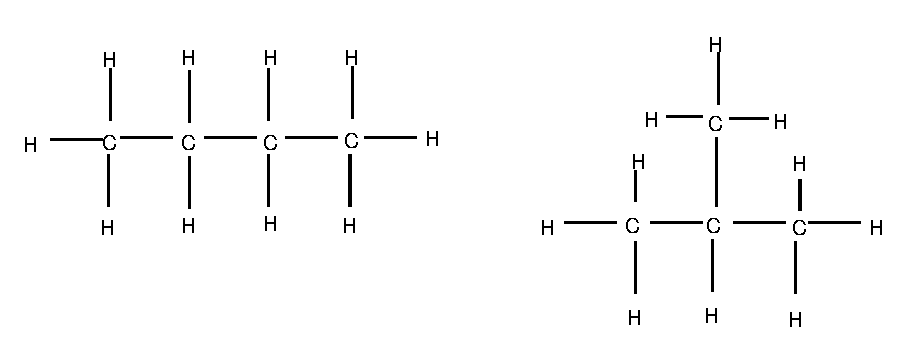
\includegraphics{../isomer_butane.eps}
 % isomer_butane.eps: 0x0 pixel, 300dpi, 0.00x0.00 cm, bb=5 2 427 155
\end{center}


% \begin{pspicture}(-3,-1.5)(4,3)
% %\psgrid[gridcolor=lightgray]
% \rput(-3,0){
% \rput(-1,0){\textbf{C}}
% \rput(0,0){\textbf{C}}
% \rput(1,0){\textbf{C}}
% \rput(2,0){\textbf{C}}
% \rput(-2.1,0){\textbf{H}}
% \rput(-1,1.1){\textbf{H}}
% \rput(-1,-1.1){\textbf{H}}
% \rput(0,1.1){\textbf{H}}
% \rput(0,-1.1){\textbf{H}}
% \rput(1,1.1){\textbf{H}}
% \rput(1,-1.1){\textbf{H}}
% \rput(2,1.1){\textbf{H}}
% \rput(2,-1.1){\textbf{H}}
% \rput(3,0){\textbf{H}}
% \psline(-1.3,0)(-1.7,0)
% \psline(-1,0.3)(-1,0.7)
% \psline(-1,-0.3)(-1,-0.7)
% \psline(-0.7,0)(-0.3,0)
% \psline(0,0.3)(0,0.7)
% \psline(0,-0.3)(0,-0.7)
% \psline(0.3,0)(0.7,0)
% \psline(1,0.3)(1,0.7)
% \psline(1,-0.3)(1,-0.7)
% \psline(1.3,0)(1.7,0)
% \psline(2,0.3)(2,0.7)
% \psline(2,-0.3)(2,-0.7)
% \psline(2.3,0)(2.7,0)
% \rput(6.5,0){
% \rput(-1,0){\textbf{C}}
% \rput(0,0){\textbf{C}}
% \rput(1,0){\textbf{C}}
% \rput(-2.1,0){\textbf{H}}
% \rput(-1,1.1){\textbf{H}}
% \rput(-1,-1.1){\textbf{H}}
% \rput(0,1.1){\textbf{H}}
% \rput(0,-1.1){\textbf{H}}
% \rput(1,-1.1){\textbf{H}}
% \psline(-1.3,0)(-1.7,0)
% \psline(-1,0.3)(-1,0.7)
% \psline(-1,-0.3)(-1,-0.7)
% \psline(-0.7,0)(-0.3,0)
% \psline(0,0.3)(0,0.7)
% \psline(0,-0.3)(0,-0.7)
% \psline(0.3,0)(0.7,0)
% \psline(1,0.3)(1,1.7)
% \psline(1,-0.3)(1,-0.7)
% \psline(1.3,0)(1.7,0)
% \rput(2,0){\textbf{H}}
% \rput(1,2){\textbf{C}}
% \psline(0.7,2)(0.3,2)
% \rput(0,2){\textbf{H}}
% \psline(1.3,2)(1.7,2)
% \rput(2,2){\textbf{H}}
% \psline(1,2.3)(1,2.7)
% \rput(1,3){\textbf{H}}
% }
% }
% \end{pspicture}
% \end{center}
\caption{Isomers of a 4-carbon organic compound}
\label{fig:organic:butane}
\end{figure}

If you were to count the number of carbon and hydrogen atoms in each compound, you would find that they are the same. They both have the same molecular formula (C$_{4}$H$_{10}$), but their structure is different and so are their properties. Such compounds are called \textbf{isomers}.

\Definition{Isomer}{
In chemistry, isomers are molecules with the same molecular formula and often with the same kinds of chemical bonds between atoms, but in which the atoms are arranged differently.
}

\Exercise{Isomers\\}{

Match the organic compound in Column A with its isomer Column B:\\

\begin{center}
\begin{tabular}{|c|c|}\hline
\textbf{Column A} & \textbf{Column B}\\\hline
CH$_{3}$CH(CH$_{3}$)OH & CH$_{3}$CH(CH$_{3}$)CH$_{3}$ \\\hline

\begin{pspicture}(0,-1.3)(5,1.3)
\rput(0,0){H}

\psline(0.3,0)(0.7,0)
\rput(1,0){C}
\psline(1,0.3)(1,0.7)
\rput(1,1){H}
\psline(1,-0.3)(1,-0.7)
\rput(1,-1){H}
\rput(1,0){
\psline(0.3,0)(0.7,0)
\rput(1,0){C}
\psline(1,0.3)(1,0.7)
\rput(1,1){H}
\psline(1,-0.3)(1,-0.7)
\rput(1,-1){H}
}
\rput(2,0){
\psline(0.3,0)(0.7,0)
\rput(1,0){C}
\psline(1,0.3)(1,0.7)
\rput(1,1){H}
\psline(1,-0.3)(1,-0.7)
\rput(1,-1){H}
}
\rput(3,0){
\psline(0.3,0)(0.7,0)
\rput(1,0){C}
\psline(1,0.3)(1,0.7)
\rput(1,1){H}
\psline(1,-0.3)(1,-0.7)
\rput(1,-1){H}
}
\psline(4.3,0)(4.7,0)
\rput(5,0){H}
\end{pspicture}

&

\begin{pspicture}(0,-1.3)(5,1.3)
\rput(0,0){H}

\psline(0.3,0)(0.7,0)
\rput(1,0){C}
\psline(1,0.3)(1,0.7)
\rput(1,1){H}
\psline(1,-0.3)(1,-0.7)
\rput(1,-1){H}
\rput(1,0){
\psline(0.3,0)(0.7,0)
\rput(1,0){C}
\psline(1,0.3)(1,0.7)
\rput(1,1){H}
\psline(1,-0.3)(1,-0.7)
\rput(1,-1){H}
}
\rput(2,0){
\psline(0.3,0)(0.7,0)
\rput(1,0){C}
\psline(1,0.3)(1,0.7)
\rput(1,1){CH$_{3}$}
\psline(1,-0.3)(1,-0.7)
\rput(1,-1){H}
}
\psline(3.3,0)(3.7,0)
\rput(4,0){H}
\end{pspicture}\\\hline

\begin{pspicture}(0,-1.3)(5,1.3)
\rput(0,0){H}

\psline(0.3,0)(0.7,0)
\rput(1,0){C}
\psline(1,0.3)(1,0.7)
\rput(1,1){CH$_{3}$}
\psline(1,-0.3)(1,-0.7)
\rput(1,-1){H}
\rput(1,0){
\psline(0.3,0)(0.7,0)
\rput(1,0){C}
\psline(1,0.3)(1,0.7)
\rput(1,1){H}
\psline(1,-0.3)(1,-0.7)
\rput(1,-1){H}
}
\rput(2,0){
\psline(0.3,0)(0.7,0)
\rput(1,0){C}
\psline(1,0.3)(1,0.7)
\rput(1,1){H}
\psline(1,-0.3)(1,-0.7)
\rput(1,-1){H}
}
\psline(3.3,0)(3.7,0)
\rput(4,0){H}
\end{pspicture}

& 

C$_{3}$H$_{7}$OH \\\hline

\end{tabular}
\end{center}
}



% CHILD SECTION END 



% CHILD SECTION START 

\section{Functional groups}
\label{sec:organic:functional}

All organic compounds have a particular bond or group of atoms which we call its \textbf{functional group}. This group is important in determining how a compound will react. 

\Definition{Functional group}{
In organic chemistry, a functional group is a specific group of atoms within molecules, that are responsible for the characteristic chemical reactions of those molecules. The same functional group will undergo the same or similar chemical reaction(s) regardless of the size of the molecule it is a part of.
}

In one group of organic compounds called the \textbf{hydrocarbons}, the single, double and triple bonds of the alkanes, alkenes and alkynes are examples of functional groups. In another group, the alcohols, an oxygen and a hydrogen atom   are bonded to each other to form the functional group for those compounds (in other words an alcohol has an OH in it). All alcohols will contain an oxygen and a hydrogen atom bonded together in some part of the molecule. \\

Table \ref{fig:om:summary} summarises some of the common functional groups. We will look at these in more detail later in this chapter.

\begin{table}[!h]
\begin{center}
\begin{tabular}{|l|c|c|c|}\hline
\textbf{Name of group} & \textbf{Functional group} & \textbf{Example} & \textbf{Diagram}\\\hline
Alk\textit{ane} & 
\begin{pspicture}(-2,-1.5)(1,1.5)
%\psgrid[gridcolor=lightgray]
\rput(-1,0){C} \rput(0,0){C} \psline(-0.8,0)(-0.2,0) \psline(0.2,0)(0.8,0)
\psline(-1.2,0)(-1.8,0)
\psline(-1,0.2)(-1,0.8)
\psline(-1,-0.2)(-1,-0.8)
\psline(0,0.2)(0,0.8)
\psline(0,-0.2)(0,-0.8)
\end{pspicture}
& Ethane &
\begin{pspicture}(-2,-1.5)(1,1.5)
%\psgrid[gridcolor=lightgray]
\rput(-1,0){C}
\rput(0,0){C}
\psline(-0.8,0)(-0.2,0)
\psline(0.2,0)(0.8,0)
\psline(-1.2,0)(-1.8,0)
\psline(-1,0.2)(-1,0.8)
\psline(-1,-0.2)(-1,-0.8)
\psline(0,0.2)(0,0.8)
\psline(0,-0.2)(0,-0.8)
\rput(-2,0){H}
\rput(1,0){H}
\rput(-1,1){H}
\rput(-1,-1){H}
\rput(0,1){H}
\rput(0,-1){H}
\end{pspicture}
\\\hline

Alk\textit{ene} & 
\begin{pspicture}(-2,-1.5)(1,1.5)
%\psgrid[gridcolor=lightgray]
\rput(-1,0){\textbf{C}}

\rput(0,0){\textbf{C}}
\psline(-0.8,-0.05)(-0.2,-0.05)
\psline(-0.8,0.05)(-0.2,0.05)
\psline(0.2,0.2)(0.7,0.7)
\psline(0.2,-0.2)(0.7,-0.7)
\psline(-1.2,0.2)(-1.7,0.7)
\psline(-1.2,-0.2)(-1.7,-0.7)
\end{pspicture} & Ethene & 

\begin{pspicture}(-2,-1.5)(1,1.5)
%\psgrid[gridcolor=lightgray]
\rput(-1,0){\textbf{C}}
\rput(0,0){\textbf{C}}
\psline(-0.8,-0.05)(-0.2,-0.05)
\psline(-0.8,0.05)(-0.2,0.05)
\psline(0.2,0.2)(0.7,0.7)
\psline(0.2,-0.2)(0.7,-0.7)
\psline(-1.2,0.2)(-1.7,0.7)
\psline(-1.2,-0.2)(-1.7,-0.7)
\rput(1,1){\textbf{H}}
\rput(1,-1){\textbf{H}}
\rput(-2,1){\textbf{H}}
\rput(-2,-1){\textbf{H}}
\end{pspicture}
\\\hline

Alk\textit{yne} & 
\begin{pspicture}(-2,-1)(1,1)
%\psgrid[gridcolor=lightgray]
\rput(-1,0){\textbf{C}}
\rput(0,0){\textbf{C}}
\psline(-1.8,0)(-1.2,0)
\psline(-0.8,0.075)(-0.2,0.075)
\psline(-0.8,0)(-0.2,0)
\psline(-0.8,-0.075)(-0.2,-0.075)
\psline(0.2,0)(0.8,0)
\end{pspicture} &
Ethyne (acetylene) & 

\begin{pspicture}(-2,-1)(1,1)
%\psgrid[gridcolor=lightgray]
\rput(-2,0){\textbf{H}}
\rput(-1,0){\textbf{C}}
\rput(0,0){\textbf{C}}
\rput(1,0){\textbf{H}}
\psline(-1.8,0)(-1.2,0)
\psline(-0.8,0.075)(-0.2,0.075)
\psline(-0.8,0)(-0.2,0)
\psline(-0.8,-0.075)(-0.2,-0.075)
\psline(0.2,0)(0.8,0)
\end{pspicture}
\\\hline

Halo-alkane & 
\begin{pspicture}(-2,-2)(0,1)
\rput(-1,0){\textbf{C}}
\rput(0,0){\textbf{X}}
\rput(-1,-1.5){(X=F,Cl,Br,I)}
\psline(-1.2,0)(-1.8,0)
\psline(-0.2,0)(-0.8,0)
\psline(-1,0.2)(-1,0.8)
\psline(-1,-0.2)(-1,-0.8)
\end{pspicture} & Chloroethane & 

\begin{pspicture}(-2,-2)(0,1.5)
\rput(-1,0){\textbf{C}}
\rput(-2.2,0){\textbf{CH$_{3}$}}
\rput(0,0){\textbf{X}}
\psline(-1.2,0)(-1.8,0)
\psline(-0.2,0)(-0.8,0)
\psline(-1,0.2)(-1,0.8)
\psline(-1,-0.2)(-1,-0.8)
\rput(-1,1){\textbf{H}}
\rput(-1,-1){\textbf{H}}
\end{pspicture}\\\hline

Alcoh\textit{ol}/ alkan\textit{ol} & 
\begin{pspicture}(-2,-2)(0,1)
\rput(-1,0){\textbf{C}}
\rput(0,0){\textbf{OH}}
\psline(-1.2,0)(-1.8,0)
\psline(-0.2,0)(-0.8,0)
\psline(-1,0.2)(-1,0.8)
\psline(-1,-0.2)(-1,-0.8)
\end{pspicture} & Ethanol & 

\begin{pspicture}(0,-1.5)(3,1.5)
\rput(0,0){\textbf{H}}
\rput(1,0){\textbf{C}}
\rput(2,0){\textbf{C}}
\rput(3,0){\textbf{H}}
\rput(1,1){\textbf{H}}
\rput(1,-1){\textbf{H}}
\rput(2,1){\textbf{OH}}
\rput(2,-1){\textbf{H}}
\rput(3,0){\textbf{H}}
\psline(0.2,0)(0.8,0)
\psline(1.2,0)(1.8,0)
\psline(2.2,0)(2.8,0)
\psline(1,0.2)(1,0.8)
\psline(1,-0.2)(1,-0.8)
\psline(2,0.2)(2,0.8)
\psline(2,-0.2)(2,-0.8)
\end{pspicture}\\\hline

Carboxylic acid & 
\begin{pspicture}(-1,-1)(1,1)
\rput(0,0){\textbf{C}}
\rput(0.6,0.6){\textbf{O}}
\rput(0.6,-0.6){\textbf{OH}}
\psline(-0.2,0)(-0.8,0)
\psline(0.05,0.2)(0.5,0.5)
\psline(-0.05,0.2)(0.4,0.5)
\psline(0,-0.2)(0.6,-0.5) 
\end{pspicture} & ethanoic acid & 

\begin{pspicture}(-2,-1)(2,1.5)
\rput(-1.7,0){\textbf{CH$_{3}$}}
\psline(-1.2,0)(-0.6,0)
\rput(-0.4,0){\textbf{C}}
\rput(-0.4,1){\textbf{O}}
\psline(-0.35,0.2)(-0.35,0.8)
\psline(-0.45,0.2)(-0.45,0.8)
\psline(-0.2,0)(0.4,0)
\rput(0.8,0){\textbf{OH}}
\end{pspicture}\\\hline

Amine & 
\begin{pspicture}(-2.5,-1)(1,1.5)
\rput(-1,0){\textbf{N}}
\rput(-2,0){\textbf{R}}
\rput(0,0.8){\textbf{H}}
\rput(0,-0.8){\textbf{H}}
\psline(-1.2,0)(-1.8,0)
\psline(-0.8,0.2)(-0.2,0.6)
\psline(-0.8,-0.2)(-0.2,-0.6)
\end{pspicture} & Glycine &

\begin{pspicture}(-2.5,-2)(2.5,2)
\rput(0,0){\textbf{C}}
\rput(0,1){\textbf{H}}
\rput(0,-1){\textbf{H}}
\rput(1,0){\textbf{N}}
\rput(2,0.8){\textbf{H}}
\rput(2,-0.8){\textbf{H}}
\rput(-1,0){\textbf{C}}
\rput(-2,0.8){\textbf{O}}
\rput(-2,-0.8){\textbf{OH}}
\psline(0,0.2)(0,0.8)
\psline(0,-0.2)(0,-0.8)
\psline(-0.2,0)(-0.8,0)
\psline(-1.15,0.2)(-1.75,0.6)
\psline(-1.25,0.2)(-1.85,0.6)
\psline(-1.2,-0.2)(-1.8,-0.6)
\psline(0.2,0)(0.8,0)
\psline(1.2,0.2)(1.8,0.6)
\psline(1.2,-0.2)(1.8,-0.6)
\end{pspicture}\\\hline

\end{tabular}
\end{center}
\caption{Some functional groups of organic compounds}
\label{fig:om:summary}
\end{table}



% CHILD SECTION END 



% CHILD SECTION START 

\section{The Hydrocarbons}
\label{sec:organic:hydrocarbons}

Let us first look at a group of organic compounds known as the \textbf{hydrocarbons}. These molecules only contain carbon and hydrogen. The hydrocarbons that we are going to look at are called \textbf{aliphatic compounds}. The aliphatic compounds are divided into \textit{acyclic compounds} (chain structures) and \textit{cyclic compounds} (ring structures). The chain structures are further divided into structures that contain only \textit{single bonds} (\textbf{alkanes}), those that contain at least one \textit{double bond} (\textbf{alkenes}) and those that contain at least one \textit{triple bond} (\textbf{alkynes}). Cyclic compounds include structures such as the \textit{benzene ring}. Figure \ref{fig:om:classhydro} summarises the classification of the hydrocarbons. \\

\begin{figure}[h]
\begin{center}
\begin{pspicture}(-8,0)(8,5)
%\psgrid[gridcolor=lightgray]
\rput(0,4){Aliphatic hydrocarbons}
\psline(0,3.8)(0,3.2)
\psline(-6,3.2)(6,3.2)
\psline(-6,3.2)(-6,2.6)
\psline(6,3.2)(6,2.6)
\rput(-6,2.5){Acyclic compounds}
\rput(-6,2.2){(chain structures)}
\rput(6,2.5){Cyclic compounds}
\rput(6,2.2){(ring structures e.g. benzene ring)}
\psline(-6,2)(-6,1.4)
\psline(-7,1.4)(4,1.4)
\psline(-7,1.4)(-7,0.8)
\psline(-2,1.4)(-2,0.8)
\psline(4,1.4)(4,0.8)
\rput(-7,0.3){Alkanes (single bonds)}
\rput(-2,0.3){Alkenes (contain double bonds)}
\rput(4,0.3){Alkynes (contain triple bonds)}
\end{pspicture}
\end{center}
\caption{The classification of the aliphatic hydrocarbons}
\label{fig:om:classhydro}
\end{figure}

Hydrocarbons that contain only single bonds are called \textbf{saturated} hydrocarbons because each carbon atom is bonded to as many hydrogen atoms as possible. Figure \ref{fig:organic:saturated} shows a molecule of ethane which is a saturated hydrocarbon.\\

\begin{figure}[!h]
\begin{center}
\begin{pspicture}(-2,-1)(1,2)
%\psgrid[gridcolor=lightgray]
\rput(-1,0){C}
\rput(0,0){C}
\psline(-0.8,0)(-0.2,0)
\psline(0.2,0)(0.8,0)
\psline(-1.2,0)(-1.8,0)
\psline(-1,0.2)(-1,0.8)
\psline(-1,-0.2)(-1,-0.8)
\psline(0,0.2)(0,0.8)
\psline(0,-0.2)(0,-0.8)
\rput(-2,0){H}
\rput(1,0){H}
\rput(-1,1){H}
\rput(-1,-1){H}
\rput(0,1){H}
\rput(0,-1){H}
\end{pspicture}
\end{center}
\caption{A saturated hydrocarbon}
\label{fig:organic:saturated}
\end{figure}

Hydrocarbons that contain double or triple bonds are called \textbf{unsaturated} hydrocarbons because they don't contain as many hydrogen atoms as possible. Figure \ref{fig:organic:unsaturated} shows a molecule of ethene which is an unsaturated hydrocarbon. If you compare the number of carbon and hydrogen atoms in a molecule of ethane and a molecule of ethene, you will see that the number of hydrogen atoms in ethene is \textit{less} than the number of hydrogen atoms in ethane despite the fact that they both contain two carbon atoms. In order for an unsaturated compound to become saturated, a double bond has to be broken, and another two hydrogen atoms added for each double bond that is replaced by a single bond.

\begin{figure}[!h]
\begin{center}
\begin{pspicture}(-2,-1)(1,2)
%\psgrid[gridcolor=lightgray]
\rput(-1,0){\textbf{C}}
\rput(0,0){\textbf{C}}
\psline(-0.8,-0.05)(-0.2,-0.05)
\psline(-0.8,0.05)(-0.2,0.05)
\psline(0.2,0.2)(0.7,0.7)
\psline(0.2,-0.2)(0.7,-0.7)
\psline(-1.2,0.2)(-1.7,0.7)
\psline(-1.2,-0.2)(-1.7,-0.7)
\rput(1,1){\textbf{H}}
\rput(1,-1){\textbf{H}}
\rput(-2,1){\textbf{H}}
\rput(-2,-1){\textbf{H}}
\end{pspicture}
\end{center}
\caption{An unsaturated hydrocarbon}
\label{fig:organic:unsaturated}
\end{figure}

\begin{IFact}{
Fat that occurs naturally in living matter such as animals and plants is used as food for human consumption and contains varying proportions of saturated and unsaturated fat. Foods that contain a high proportion of saturated fat are butter, ghee, suet, tallow, lard, coconut oil, cottonseed oil, and palm kernel oil, dairy products (especially cream and cheese), meat, and some prepared foods. Diets high in saturated fat are correlated with an increased incidence of atherosclerosis and coronary heart disease according to a number of studies. Vegetable oils contain unsaturated fats and can be hardened to form margarine by adding hydrogen on to some of the carbon=carbon double bonds using a nickel catalyst. The process is called hydrogenation
}
\end{IFact}

We will now go on to look at each of the hydrocarbon groups in more detail. These groups are the alkanes, the alkenes and the alkynes.

\subsection{The Alkanes}

The alkanes are hydrocarbons that only contain \textit{single covalent bonds} between their carbon atoms. This means that they are \textit{saturated} compounds and are quite unreactive. The simplest alkane has only one carbon atom and is called \textbf{methane}. This molecule is shown in figure \ref{fig:organic:methane}.

\begin{figure}[!h]
\begin{center}
\begin{pspicture}(-3,-1)(3,1.5)
%\psgrid[gridcolor=lightgray]
\rput(-1,0){\textbf{C}}
\rput(-2,0){\textbf{H}}
\rput(0,0){\textbf{H}}
\rput(-1,1){\textbf{H}}
\rput(-1,-1){\textbf{H}}
\psline(-0.2,0)(-0.8,0)
\psline(-1.2,0)(-1.8,0)
\psline(-1,0.2)(-1,0.8)
\psline(-1,-0.2)(-1,-0.8)
\rput(-2.8,0){\textbf{(a)}}
\rput(1,0){\textbf{(b)}}
\rput(2,0){\textbf{CH$_{4}$}}
\end{pspicture}
\end{center}
\caption{The structural (a) and molecular formula (b) for methane}
\label{fig:organic:methane}
\end{figure}

The second alkane in the series has two carbon atoms and is called \textbf{ethane}. This is shown in figure \ref{fig:organic:ethane}.\\

\begin{figure}[!h]
\begin{center}
\begin{pspicture}(-3,-1)(5,1.5)
%\psgrid[gridcolor=lightgray]
\rput(-1,0){\textbf{C}}
\rput(-2,0){\textbf{H}}
\rput(-1,1){\textbf{H}}
\rput(-1,-1){\textbf{H}}
\rput(0,0){\textbf{C}}
\rput(1,0){\textbf{H}}
\rput(0,1){\textbf{H}}
\rput(0,-1){\textbf{H}}
\psline(-0.2,0)(-0.8,0)
\psline(-1.2,0)(-1.8,0)
\psline(-1,0.2)(-1,0.8)
\psline(-1,-0.2)(-1,-0.8)
\psline(0.2,0)(0.8,0)
\psline(0,0.2)(0,0.8)
\psline(0,-0.2)(0,-0.8)
\rput(-2.8,0){\textbf{(a)}}
\rput(3,0){\textbf{(b)}}
\rput(4,0){\textbf{C$_{2}$H$_{6}$}}
\end{pspicture}
\end{center}
\caption{The structural (a) and molecular formula (b) for ethane}
\label{fig:organic:ethane}
\end{figure}

The third alkane in the series has three carbon atoms and is called \textbf{propane} (Figure \ref{fig:organic:propane}).

\begin{figure}[!h]
\begin{center}
\begin{pspicture}(-3,-1)(5,1.5)
%\psgrid[gridcolor=lightgray]
\rput(-1,0){\textbf{C}}
\rput(-2,0){\textbf{H}}
\rput(-1,1){\textbf{H}}
\rput(-1,-1){\textbf{H}}
\rput(0,0){\textbf{C}}
\rput(0,1){\textbf{H}}
\rput(0,-1){\textbf{H}}
\rput(1,0){\textbf{C}}
\rput(2,0){\textbf{H}}
\rput(1,1){\textbf{H}}
\rput(1,-1){\textbf{H}}
\psline(-0.2,0)(-0.8,0)
\psline(-1.2,0)(-1.8,0)
\psline(-1,0.2)(-1,0.8)
\psline(-1,-0.2)(-1,-0.8)
\psline(0.2,0)(0.8,0)
\psline(0,0.2)(0,0.8)
\psline(0,-0.2)(0,-0.8)
\psline(1.2,0)(1.8,0)
\psline(1,0.2)(1,0.8)
\psline(1,-0.2)(1,-0.8)
\rput(-2.8,0){\textbf{(a)}}
\rput(3,0){\textbf{(b)}}
\rput(4,0){\textbf{C$_{3}$H$_{8}$}}
\end{pspicture}
\end{center}
\caption{The structural (a) and molecular formula (b) for propane}
\label{fig:organic:propane}
\end{figure}

When you look at the molecular formula for each of the alkanes, you should notice a pattern developing. For each carbon atom that is added to the molecule, two hydrogen atoms are added. In other words, each molecule differs from the one before it by CH$_{2}$. This is called a \textit{homologous series}. The alkanes have the general formula C$_{n}$H$_{2n+2}$.

The alkanes are the most important source of fuel in the world and are used extensively in the chemical industry. Some are gases (e.g. methane and ethane), while others are liquid fuels (e.g. octane, an important component of petrol).

\begin{IFact}{Some fungi use alkanes as a source of carbon and energy. One fungus \textit{Amorphotheca resinae} prefers the alkanes used in aviation fuel, and this can cause problems for aircraft in tropical areas!}
\end{IFact}

\subsection{Naming the alkanes}

In order to give compounds a name, certain rules must be followed. When naming organic compounds, the IUPAC (International Union of Pure and Applied Chemistry) nomenclature is used. We will first look at some of the steps that need to be followed when naming a compound, and then try to apply these rules to some specific examples.

\begin{enumerate}
\item{STEP 1: Recognise the \textit{functional group} in the compound. This will determine the suffix (the 'end') of the name. For example, if the compound is an alkane, the suffix will be -ane; if the compound is an alkene the suffix will be -ene; if the compound is an alcohol the suffix will be -ol, and so on.}
\item{STEP 2: Find the longest continuous carbon chain (it won't always be a \textit{straight} chain) and count the number of carbon atoms in this chain. This number will determine the prefix (the 'beginning') of the compound's name. These prefixes are shown in table \ref{tab:prefix}. So, for example, an alkane that has 3 carbon atoms will have the suffix \textit{prop} and the compound's name will be \textit{propane}.

\begin{table}[!h]
\begin{center}
\begin{tabular}{|c|c|}\hline
\textbf{Carbon atoms} & prefix \\\hline

1 & meth(ane)\\\hline
2 & eth(ane)\\\hline
3 & prop(ane)\\\hline
4 & but(ane) \\\hline
5 & pent(ane) \\\hline
6 & hex(ane) \\\hline
7 & hept(ane) \\\hline
8 & oct(ane) \\\hline
9 & non(ane) \\\hline
10 & dec(ane) \\\hline
\end{tabular}
\end{center}
\caption{The prefix of a compound's name is determined by the number of carbon atoms in the longest chain}
\label{tab:prefix}
\end{table}
}
\item{STEP 3: Number the carbons in the longest carbon chain (Important: If there is a double or triple bond, you need to start numbering so that the bond is at the carbon with the lowest number.}
\item{STEP 4: Look for any branched groups and name them. Also give them a number to show their position on the carbon chain. If there are no branched groups, this step can be left out.}
\item{STEP 5: Combine the elements of the name into a single word in the following order: branched groups; prefix; name ending according to the functional group and its position along the longest carbon chain.}
\end{enumerate}
Khan Academy video on naming simple alkanes: SIYAVULA-VIDEO:http://cnx.org/content/m39453/latest/#alkanes-1
\begin{wex}{Naming the alkanes}{Give the IUPAC name for the following compound:
\begin{figure}[H]
\begin{center}
\begin{pspicture}(-3,-1.5)(4,1.5)
%\psgrid[gridcolor=lightgray]
\rput(-1,0){\textbf{C$_{(1)}$}}
\rput(-2,0){\textbf{H}}
\rput(-1,1){\textbf{H}}
\rput(-1,-1){\textbf{H}}
\rput(0,0){\textbf{C$_{(2)}$}}
\rput(0,1){\textbf{H}}
\rput(0,-1){\textbf{H}}
\rput(1,0){\textbf{C$_{(3)}$}}
\rput(2,0){\textbf{C$_{(4)}$}}
\rput(1,1){\textbf{H}}
\rput(1,-1){\textbf{H}}
\psline(-0.2,0)(-0.8,0)
\psline(-1.2,0)(-1.8,0)
\psline(-1,0.2)(-1,0.8)
\psline(-1,-0.2)(-1,-0.8)
\psline(0.2,0)(0.8,0)
\psline(0,0.2)(0,0.8)
\psline(0,-0.2)(0,-0.8)
\psline(1.2,0)(1.8,0)
\psline(1,0.2)(1,0.8)
\psline(1,-0.2)(1,-0.8)
\rput(2,1){\textbf{H}}
\rput(2,-1){\textbf{H}}
\rput(3,0){\textbf{H}}
\psline(2.2,0)(2.8,0)
\psline(2,0.2)(2,0.8)
\psline(2,-0.2)(2,-0.8)
\end{pspicture}
\end{center}
\end{figure}
Note: The numbers attached to the carbon atoms would not normally be shown. The atoms have been numbered to help you to name the compound.
}
{\westep{Identify the functional group}
The compound is a hydrocarbon with single bonds between the carbon atoms. It is an alkane and will have a suffix of -ane.

\westep{Find the longest carbon chain}
There are four carbon atoms in the longest chain. The prefix of the compound will be 'but'.
\westep{Number the carbons in the longest chain}
In this case, it is easy. The carbons are numbered from left to right, from one to four.
\westep{Look for any branched groups, name them and give their position on the carbon chain}
There are no branched groups in this compound.
\westep{Combine the elements of the name into a single word}
The name of the compound is \textbf{butane}.
}
\end{wex}

\begin{wex}{Naming the alkanes}{Give the IUPAC name for the following compound:
\begin{figure}[H]
\begin{center}
\begin{pspicture}(-3,-3.5)(3,1.5)
%\psgrid[gridcolor=lightgray]
\rput(-1,0){\textbf{C}}
\rput(0,0){\textbf{C}}
\rput(1,0){\textbf{C}}
\rput(-2,0){\textbf{H}}
\rput(2,0){\textbf{H}}
\rput(-1,1){\textbf{H}}
\rput(-1,-1){\textbf{H}}
\rput(0,1){\textbf{H}}
\rput(1,1){\textbf{H}}
\rput(1,-1){\textbf{H}}
\rput(0,-2){\textbf{C}}
\rput(0,-3){\textbf{H}}
\rput(-1,-2){\textbf{H}}
\rput(1,-2){\textbf{H}}
\psline(-1.8,0)(-1.2,0)
\psline(-0.8,0)(-0.2,0)
\psline(0.8,0)(0.2,0)
\psline(1.8,0)(1.2,0)
\psline(-1,0.2)(-1,0.8)
\psline(-1,-0.2)(-1,-0.8)
\psline(0,0.2)(0,0.8)
\psline(0,-0.2)(0,-1.8)
\psline(1,0.2)(1,0.8)
\psline(1,-0.2)(1,-0.8)
\psline(-0.8,-2)(-0.2,-2)
\psline(0.2,-2)(0.8,-2)
\psline(0,-2.2)(0,-2.8)
\end{pspicture}
\end{center}
\end{figure}
}
{\westep{Identify the functional group}
The compound is an alkane and will have the suffix -ane.
\westep{Find the longest carbon chain}
There are three carbons in the longest chain. The prefix for this compound is -prop. 
\westep{Number the carbons in the carbon chain}
If we start at the carbon on the left, we can number the atoms as shown below:
\begin{figure}[H]
\begin{center}
\begin{pspicture}(-3,-3.5)(3,1.5)
%\psgrid[gridcolor=lightgray]
\rput(-1,0){\textbf{C$_{(1)}$}}
\rput(0,0){\textbf{C$_{(2)}$}}
\rput(1,0){\textbf{C$_{(3)}$}}
\rput(-2,0){\textbf{H}}
\rput(2,0){\textbf{H}}
\rput(-1,1){\textbf{H}}
\rput(-1,-1){\textbf{H}}
\rput(0,1){\textbf{H}}
\rput(1,1){\textbf{H}}
\rput(1,-1){\textbf{H}}
\rput(0,-2){\textbf{C}}
\rput(0,-3){\textbf{H}}
\rput(-1,-2){\textbf{H}}
\rput(1,-2){\textbf{H}}
\psline(-1.8,0)(-1.2,0)
\psline(-0.8,0)(-0.2,0)
\psline(0.8,0)(0.2,0)
\psline(1.8,0)(1.2,0)
\psline(-1,0.2)(-1,0.8)
\psline(-1,-0.2)(-1,-0.8)
\psline(0,0.2)(0,0.8)
\psline(0,-0.2)(0,-1.8)
\psline(1,0.2)(1,0.8)
\psline(1,-0.2)(1,-0.8)
\psline(-0.8,-2)(-0.2,-2)
\psline(0.2,-2)(0.8,-2)
\psline(0,-2.2)(0,-2.8)
\end{pspicture}
\end{center}
\end{figure}
\westep{Look for any branched groups, name them and give their position on the carbon chain}
There is a branched group attached to the second carbon atom. This group has the formula CH$_{3}$ which is methane. However, because it is not part of the main chain, it is given the suffix -yl (i.e. methyl). The position of the methyl group comes just before its name (see next step).
\westep{Combine the elements of the compound's name into a single word in the order of branched groups; prefix; name ending according to the functional group.}
The compound's name is \textbf{2-methylpropane}.
}
\end{wex}

\begin{wex}{Naming the alkanes}{Give the IUPAC name for the following compound:
\begin{center}
CH$_{3}$CH(CH$_{3}$)CH(CH$_{3}$)CH$_{3}$
\end{center}
(Remember that the side groups are shown in brackets after the carbon atom to which they are attached.)
}{
\westep{Draw the compound from its condensed structural formula}
The structural formula of the compound is:
\begin{figure}[H]
\begin{center}
\begin{pspicture}(-3,-0.7)(4,1)
%\psgrid[gridcolor=lightgray]
\rput(-1,0){\textbf{C$_{(1)}$}}
\rput(-2,0){\textbf{H}}
\rput(-1,1){\textbf{H}}
\rput(-1,-1){\textbf{H}}
\rput(0,0){\textbf{C$_{(2)}$}}
\rput(0,1){\textbf{CH$_{3}$}}
\rput(0,-1){\textbf{H}}
\rput(1,0){\textbf{C$_{(3)}$}}
\rput(2,0){\textbf{C$_{(4)}$}}
\rput(1,1){\textbf{CH$_{3}$}}
\rput(1,-1){\textbf{H}}
\psline(-0.2,0)(-0.8,0)
\psline(-1.2,0)(-1.8,0)
\psline(-1,0.2)(-1,0.8)
\psline(-1,-0.2)(-1,-0.8)
\psline(0.2,0)(0.8,0)
\psline(0,0.2)(0,0.8)
\psline(0,-0.2)(0,-0.8)
\psline(1.2,0)(1.8,0)
\psline(1,0.2)(1,0.8)
\psline(1,-0.2)(1,-0.8)
\rput(2,1){\textbf{H}}
\rput(2,-1){\textbf{H}}
\rput(3,0){\textbf{H}}
\psline(2.2,0)(2.8,0)
\psline(2,0.2)(2,0.8)
\psline(2,-0.2)(2,-0.8)
\end{pspicture}
\end{center}
\end{figure}
\westep{Identify the functional group}
The compound is an alkane and will have the suffix -ane.
\westep{Find the longest carbon chain}
There are four carbons in the longest chain. The prefix for this compound is -but. 
\westep{Number the carbons in the carbon chain}
If we start at the carbon on the left, carbon atoms are numbered as shown in the diagram above. A second way that the carbons could be numbered is:
\begin{figure}[H]
\begin{center}
\begin{pspicture}(-3,-0.7)(4,1)
%\psgrid[gridcolor=lightgray]
\rput(-1,0){\textbf{C$_{(1)}$}}
\rput(-2,0){\textbf{H}}
\rput(-1,1){\textbf{H}}
\rput(-1,-1){\textbf{H}}
\rput(0,0){\textbf{C$_{(2)}$}}
\rput(0,1){\textbf{CH$_{3}$}}
\rput(0,-1){\textbf{H}}
\rput(1,0){\textbf{C$_{(3)}$}}
\rput(2,0){\textbf{C}}
\rput(1,1){\textbf{CH$_{3 (4)}$}}
\rput(1,-1){\textbf{H}}
\psline(-0.2,0)(-0.8,0)
\psline(-1.2,0)(-1.8,0)
\psline(-1,0.2)(-1,0.8)
\psline(-1,-0.2)(-1,-0.8)
\psline(0.2,0)(0.8,0)
\psline(0,0.2)(0,0.8)
\psline(0,-0.2)(0,-0.8)
\psline(1.2,0)(1.8,0)
\psline(1,0.2)(1,0.8)
\psline(1,-0.2)(1,-0.8)
\rput(2,1){\textbf{H}}
\rput(2,-1){\textbf{H}}
\rput(3,0){\textbf{H}}
\psline(2.2,0)(2.8,0)
\psline(2,0.2)(2,0.8)
\psline(2,-0.2)(2,-0.8)
\end{pspicture}
\end{center}
\end{figure}
\westep{Look for any branched groups, name them and give their position on the carbon chain}
There are two methyl groups attached to the main chain. The first one is attached to the second carbon atom and the second methyl group is attached to the third carbon atom. Notice that in this example it does not matter how you have chosen to number the carbons in the main chain; the methyl groups are still attached to the second and third carbons and so the naming of the compound is not affected.
\westep{Combine the elements of the compound's name into a single word in the order of branched groups; prefix; name ending according to the functional group.}
The compound's name is \textbf{2,3-dimethyl-butane}.}
\end{wex}

\begin{wex}{Naming the alkanes}{Give the IUPAC name for the following compound:
\begin{figure}[H]
\begin{center}
\begin{pspicture}(-3,-2)(4,1)
%\psgrid[gridcolor=lightgray]
\rput(-1,0){\textbf{C}}
\rput(-2,0){\textbf{H}}
\rput(-1,1){\textbf{CH$_{3}$}}
\rput(-1,-1){\textbf{H}}
\rput(0,0){\textbf{C}}
\rput(0,1){\textbf{H}}
\rput(0,-1){\textbf{H}}
\rput(1,0){\textbf{C}}
\rput(2,0){\textbf{C}}
\rput(1,1){\textbf{H}}
\rput(1,-1){\textbf{CH$_{2}$}}
\psline(1,-1.3)(1,-1.7)
\rput(1,-2){\textbf{CH$_{3}$}}
\psline(-0.2,0)(-0.8,0)
\psline(-1.2,0)(-1.8,0)
\psline(-1,0.2)(-1,0.8)
\psline(-1,-0.2)(-1,-0.8)
\psline(0.2,0)(0.8,0)
\psline(0,0.2)(0,0.8)
\psline(0,-0.2)(0,-0.8)
\psline(1.2,0)(1.8,0)
\psline(1,0.2)(1,0.8)
\psline(1,-0.2)(1,-0.8)
\rput(2,1){\textbf{H}}
\rput(2,-1){\textbf{H}}
\rput(3,0){\textbf{H}}
\psline(2.2,0)(2.8,0)
\psline(2,0.2)(2,0.8)
\psline(2,-0.2)(2,-0.8)
\end{pspicture}
\end{center}
\end{figure}
}{\westep{Identify the functional group}
The compound is an alkane and will have the suffix -ane.

\westep{Find the longest carbon chain and number the carbons in the longest chain.}
There are six carbons in the longest chain if they are numbered as shown below. The prefix for the compound is hex-.

\begin{figure}[H]
\begin{center}
\begin{pspicture}(-3,-2)(4,1)
%\psgrid[gridcolor=lightgray]
\rput(-1,0){\textbf{C$_{(5)}$}}
\rput(-2,0){\textbf{H}}
\rput(-1,1){\textbf{CH$_{3 (6)}$}}
\rput(-1,-1){\textbf{H}}
\rput(0,0){\textbf{C$_{(4)}$}}
\rput(0,1){\textbf{H}}
\rput(0,-1){\textbf{H}}
\rput(1,0){\textbf{C$_{(3)}$}}
\rput(2,0){\textbf{C}}
\rput(1,1){\textbf{H}}
\rput(1,-1){\textbf{CH$_{2 (2)}$}}
\psline(1,-1.3)(1,-1.7)
\rput(1,-2){\textbf{CH$_{3 (1)}$}}
\psline(-0.2,0)(-0.8,0)
\psline(-1.2,0)(-1.8,0)
\psline(-1,0.2)(-1,0.8)
\psline(-1,-0.2)(-1,-0.8)
\psline(0.2,0)(0.8,0)
\psline(0,0.2)(0,0.8)
\psline(0,-0.2)(0,-0.8)
\psline(1.2,0)(1.8,0)
\psline(1,0.2)(1,0.8)
\psline(1,-0.2)(1,-0.8)
\rput(2,1){\textbf{H}}
\rput(2,-1){\textbf{H}}
\rput(3,0){\textbf{H}}
\psline(2.2,0)(2.8,0)
\psline(2,0.2)(2,0.8)
\psline(2,-0.2)(2,-0.8)
\end{pspicture}
\end{center}
\end{figure}
 \westep{Look for any branched groups, name them and give their position on the carbon chain}
There is one methyl group attached to the main chain. This is attached to the third carbon atom. 
\westep{Combine the elements of the compound's name into a single word in the order of branched groups; prefix; name ending according to the functional group.}
The compound's name is \textbf{3-methyl-hexane}.
}
\end{wex}


\Exercise{Naming the alkanes\\}{
\begin{enumerate}
\item{Give the structural formula for each of the following:}
	\begin{enumerate}
	\item{Octane}
	\item{CH$_{3}$CH$_{2}$CH$_{3}$}
	\item{CH$_{3}$CH(CH$_{3}$)CH$_{3}$}
	\item{3-ethyl-pentane}
	\end{enumerate}

\item{Give the IUPAC name for each of the following organic compounds.}
	\begin{enumerate}
	\item{\begin{pspicture}(0,-1.3)(5,1.3)
\rput(0,0){H}

\psline(0.3,0)(0.7,0)
\rput(1,0){C}
\psline(1,0.3)(1,0.7)
\rput(1,1){H}
\psline(1,-0.3)(1,-0.7)
\rput(1,-1){H}
\rput(1,0){
\psline(0.3,0)(0.7,0)
\rput(1,0){C}
\psline(1,0.3)(1,0.7)
\rput(1,1){H}
\psline(1,-0.3)(1,-0.7)
\rput(1,-1){H}
}
\rput(2,0){
\psline(0.3,0)(0.7,0)
\rput(1,0){C}
\psline(1,0.3)(1,0.7)
\rput(1,1){CH$_{3}$}
\psline(1,-0.3)(1,-0.7)
\rput(1,-1){H}
}
\psline(3.3,0)(3.7,0)
\rput(4,0){H}
\end{pspicture}
}

\item{CH$_{3}$CH$_{2}$CH(CH$_{3}$)CH$_{2}$CH$_{3}$}
\item{CH$_{3}$CH(CH$_{3}$)CH$_{2}$CH(CH$_{3}$)CH$_{3}$}
	\end{enumerate}
\end{enumerate}
}

\subsection{Properties of the alkanes}

We have already mentioned that the alkanes are relatively unreactive because of their stable C-C and C-H bonds. The boiling point and melting point of these molecules is determined by their molecular structure, and their surface area. The more carbon atoms there are in an alkane, the greater the surface area and therefore the higher the boiling point. The melting point also increases as the number of carbon atoms in the molecule increases. This can be seen in the data in table \ref{fig:alkane properties}.

\begin{table}[h]
\begin{center}
\begin{tabular}{|l|l|c|c|c|}\hline
\textbf{Formula} & \textbf{Name} & \textbf{Melting point ($^{0}$C)} & \textbf{Boiling point ($^{0}$C)} & \textbf{Phase at room temperature}\\\hline
CH$_{4}$ & methane & -183 & -162 & gas\\\hline
C$_{2}$H$_{6}$ & ethane & -182 & -88  & gas\\\hline
C$_{3}$H$_{8}$ & propane & -187 & -45 & gas \\\hline
C$_{4}$H$_{10}$ & butane & -138 & -0.5 & gas \\\hline
C$_{5}$H$_{12}$ & pentane & -130 & 36 & liquid \\\hline
C$_{6}$H$_{14}$ & hexane & -95 & 69 & liquid \\\hline
C$_{17}$H$_{36}$ & heptadecane & 22 & 302 & solid \\\hline
\end{tabular}
\caption{Properties of some of the alkanes}
\label{fig:alkane properties}
\end{center}
\end{table}

You will also notice that, when the molecular mass of the alkanes is low (i.e. there are few carbon atoms), the organic compounds are \textit{gases} because the intermolecular forces are weak. As the number of carbon atoms and the molecular mass increases, the compounds are more likely to be liquids or solids because the intermolecular forces are stronger.

\subsection{Reactions of the alkanes}

There are three types of reactions that can occur in saturated compounds such as the alkanes.

\begin{enumerate}
\item{\textbf{Substitution reactions}

Substitution reactions involve the removal of a hydrogen atom which is replaced by an atom of another element, such as a halogen (F, Cl, Br or I) (figure \ref{fig:organic:substitution}). The product is called a \textbf{halo-alkane}. Since alkanes are not very reactive, either heat or light is needed for this reaction to take place.\\

e.g. CH$_{2}$=CH$_{2}$ + HBr \rm${\rightarrow}$ CH$_{3}$-CH$_{2}$-Br (halo-alkane)

\begin{figure}[h]

\begin{center}
 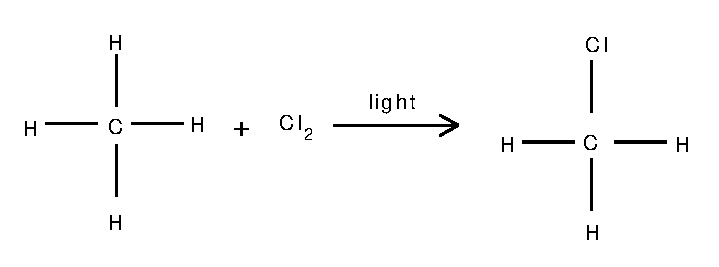
\includegraphics{../substitution_rxn.eps}
 % substitution_rxn.eps: 0x0 pixel, 300dpi, 0.00x0.00 cm, bb=3 6 332 118
\end{center}


% \begin{center}
% \begin{pspicture}(-2,-1)(10,1)
% \rput(-1,0){\textbf{H}}
% \psline(-0.7,0)(-0.3,0)
% \rput(0,0){\textbf{C}}
% \psline(0,0.3)(0,0.7)
% \rput(0,1){\textbf{H}}
% \psline(0.3,0.05)(0.7,0.05)
% \psline(0.3,-0.05)(0.7,-0.05)
% \rput(1,0){\textbf{C}}
% \psline(1,0.3)(1,0.7)
% \rput(1,1){\textbf{H}}
% \psline(1.3,0)(1.7,0)
% \rput(2,0){\textbf{H}}
% \rput(3,0){\textbf{+}}
% \rput(4,0){\textbf{HBr}}
% \psline[arrows=->](4.7,0)(5.5,0)
% \rput(7,0){
% \rput(-1,0){\textbf{H}}
% \psline(-0.7,0)(-0.3,0)
% \rput(0,0){\textbf{C}}
% \psline(0,0.3)(0,0.7)
% \rput(0,1){\textbf{H}}
% \psline(0.3,0)(0.7,0)
% \rput(1,0){\textbf{C}}
% \psline(1,0.3)(1,0.7)
% \rput(1,1){\textbf{H}}
% \psline(1.3,0)(1.7,0)
% \rput(2,0){\textbf{Br}}
% \rput(0,-1){\textbf{H}}
% \rput(1,-1){\textbf{H}}
% \psline(0,-0.3)(0,-0.7)
% \psline(1,-0.3)(1,-0.7)
% }
% \end{pspicture}
% \end{center}
\caption{A substitution reaction}
\label{fig:organic:substitution}
\end{figure}
}

Halo-alkanes (also sometimes called \textit{alkyl halides}) that contain methane and chlorine are substances that can be used as anaesthetics during operations. One example is trichloromethane, also known as 'chloroform' (figure \ref{fig:om:chloroform}).

\begin{figure}[h]
\begin{center}
\begin{pspicture}(-1.5,-1.5)(3,1.5)
%\psgrid[gridcolor=lightgray]
\rput(0,0){\textbf{C}}
\rput(1,1){\textbf{Cl}}
\rput(-1,1){\textbf{H}}
\rput(-1,-1){\textbf{Cl}}
\rput(1,-1){\textbf{Cl}}
\psline(0.2,0.2)(0.8,0.8)
\psline(-0.2,0.2)(-0.8,0.8)
\psline(0.2,-0.2)(0.8,-0.8)
\psline(-0.2,-0.2)(-0.8,-0.8)
\rput(2.5,0){\textbf{CHCl$_{3}$}}
\end{pspicture}

\end{center}
\caption{Trichloromethane}
\label{fig:om:chloroform}
\end{figure}


\item{\textbf{Elimination reactions}

Saturated compounds can also undergo elimination reactions to become unsaturated (figure \ref{fig:organic:elimination}). In the example below, an atom of hydrogen and chlorine are eliminated from the original compound to form an unsaturated halo-alkene.\\

e.g. \rm${ClH_{2}C-CH_{2}Cl \rightarrow H_{2}C=CHCl + HCl}$

\begin{figure}[h]
\begin{center}
\begin{pspicture}(-3,-1)(10,2)
\rput(-1,0){\textbf{H}}
\psline(-0.7,0)(-0.3,0)
\rput(0,0){\textbf{C}}
\psline(0,0.3)(0,0.7)
\rput(0,1){\textbf{H}}
\psline(0.3,0)(0.7,0)
\rput(1,0){\textbf{C}}
\psline(1,0.3)(1,0.7)
\rput(1,1){\textbf{H}}
\psline(1.3,0)(1.7,0)
\rput(2,0){\textbf{}}
\rput(0,-1){\textbf{Cl}}
\rput(1,-1){\textbf{Cl}}
\psline(0,-0.3)(0,-0.7)
\psline(1,-0.3)(1,-0.7)
\rput(2,0){\textbf{H}}
\psline[arrows=->](2.7,0)(3.5,0)
\rput(5,0){
\rput(-1,0){\textbf{H}}
\psline(-0.7,0)(-0.3,0)
\rput(0,0){\textbf{C}}
\psline(0,0.3)(0,0.7)
\rput(0,1){\textbf{H}}
\psline(0.3,0.05)(0.7,0.05)
\psline(0.3,-0.05)(0.7,-0.05)
\rput(1,0){\textbf{C}}
\psline(1,0.3)(1,0.7)
\rput(1,1){\textbf{H}}
\psline(1.3,0)(1.7,0)
\rput(2,0){\textbf{Cl}}
\rput(3,0){\textbf{+}}
\rput(4,0){\textbf{HCl}}
}
\end{pspicture}
\end{center}
\caption{An elimination reaction}
\label{fig:organic:elimination}
\end{figure}
}
\item{\textbf{Oxidation reactions}
 
When alkanes are burnt in air, they react with the oxygen in air and heat is produced. This is called an oxidation or combustion reaction. Carbon dioxide and water are given off as products. Heat is also released during the reaction. The burning of alkanes provides most of the energy that is used by man.\\

e.g. \rm${CH_{4} + 2O_{2} \rightarrow CO_{2} + 2H_{2}O + heat}$
}

\end{enumerate}


\Exercise{The Alkanes}{

\begin{enumerate}
\item{Give the IUPAC name for each of the following alkanes:}
	\begin{enumerate}
	\item{CH$_{3}$CH$_{2}$CH$_{2}$CH$_{2}$CH$_{2}$CH$_{3}$}
	\item{
	\begin{pspicture}(-3,-1.5)(2,3.5)
	%\psgrid[gridcolor=lightgray]
	\rput(-2,0){\textbf{C}}
	\rput(-2,1){\textbf{H}}
	\rput(-2,-1){\textbf{H}}
	\rput(-3,0){\textbf{H}}


	\psline(-2.8,0)(-2.2,0)
	\psline(-2,0.2)(-2,0.8)
	\psline(-2,-0.2)(-2,-0.8)
	\psline(-1.8,0)(-1.2,0)
	\rput(-1,0){\textbf{C}}
	\psline(-0.8,0)(-0.2,0)
	\rput(0,0){\textbf{C}}
	\psline(0.2,0)(0.8,0)
	\rput(1,0){\textbf{C}}
	\psline(1.2,0)(1.8,0)
	\psline(-1,0.2)(-1,1.8)
	\rput(-1,2){\textbf{C}}
	\rput(-1,3){\textbf{H}}
	\psline(-1.2,2)(-1.8,2)
	\psline(-0.2,2)(-0.8,2)
	\psline(-1,2.2)(-1,2.8)
	\rput(-2,2){\textbf{H}}
	\rput(0,2){\textbf{H}}
	\psline(-1,-0.2)(-1,-0.8)
	\rput(-1,-1){\textbf{H}}
	\rput(0,1){\textbf{H}}
	\rput(0,-1){\textbf{H}}
	\psline(0,0.2)(0,0.8)
	\psline(0,-0.2)(0,-0.8)
	\psline(1,0.2)(1,0.8)
	\rput(1,1){\textbf{H}}
	\psline(1,-0.2)(1,-0.8)
	\rput(1,-1){\textbf{H}}
	\rput(2,0){\textbf{H}}
	\end{pspicture}
	}
\item{CH$_{3}$CH$_{3}$}
\end{enumerate}

\item{Give the structural formula for each of the following compounds:}
	\begin{enumerate}
	\item{octane}
	\item{3-methyl-hexane}
	\end{enumerate}


\item{Methane is one of the simplest alkanes and yet it is an important fuel source. Methane occurs naturally in wetlands, natural gas and permafrost. However, methane can also be produced when organic wastes (e.g. animal manure and decaying material) are broken down by bacteria under conditions that are anaerobic (there is no oxygen). The simplified reaction is shown below:

\begin{center}
Organic matter \rm${\rightarrow}$ Simple organic acids \rm${\rightarrow}$ Biogas
\end{center}

The organic matter could be carbohydrates, proteins or fats which are broken down by acid-forming bacteria into simple organic acids such as acetic acid or formic acid. Methane-forming bacteria then convert these acids into biogases such as methane and ammonia.\\

The production of methane in this way is very important because methane can be used as a fuel source. One of the advantages of methane over other fuels like coal, is that it produces more energy but with lower carbon dioxide emissions. The problem however, is that methane itself is a greenhouse gas and has a much higher global warming potential than carbon dioxide. So, producing methane may in fact have an even more dangerous impact on the environment.

\begin{enumerate}
\item{What is the structural formula of methane?}
\item{Write an equation to show the reaction that takes place when methane is burned as a fuel.}
\item{Explain what is meant by the statement that methane 'has a greater global warming potential than carbon dioxide'.}
\end{enumerate}
}

\item{Chlorine and ethane react to form chloroethane and hydrogen chloride.}
	\begin{enumerate}
	\item{Write a balanced chemical equation for this reaction, using molecular formulae.}
	\item{Give the structural formula of chloroethane.}
	\item{What type of reaction has taken place in this example?}
	\end{enumerate}

\item{Petrol (C$_{8}$H$_{18}$) is in fact not pure C$_{8}$H$_{18}$ but a mixture of various \textit{alkanes}. The 'octane rating' of petrol refers to the percentage of the petrol which is C$_{8}$H$_{18}$. For example, 93 octane fuel contains 93\% C$_{8}$H$_{18}$ and 7\% other alkanes. The \textit{isomer} of C$_{8}$H$_{18}$ referred to in the 'octane rating' is in fact not octane but 2,2,4-trimethylpentane.}
	\begin{enumerate}
	\item{Write an unbalanced equation for the chemical reaction which takes place when petrol (C$_{8}$H$_{18}$) burns in excess oxygen.}
	\item{Write the general formula of the \textit{alkanes}.}
	\item{Define the term \textit{structural isomer}.}
	\item{Use the information given in this question and your knowledge of naming organic compounds to deduce and draw the full structural formula for 2,2,4-trimethylpentane.}
(IEB pg 25) 
	\end{enumerate}
\end{enumerate}

}

\subsection{The alkenes}

In the alkenes, there is at least one double bond between two carbon atoms. This means that they are \textbf{unsaturated} and are \textit{more reactive} than the alkanes. The simplest alkene is ethene (also known as ethylene), which is shown in figure \ref{fig:om:ethene3rep}.

\begin{figure}[h]
\begin{center}

\begin{pspicture}(-3,-1)(8,2)
%\psgrid[gridcolor=lightgray]
\rput(-3,0){(a)}
\rput(-1,0){\textbf{C}}
\rput(0,0){\textbf{C}}
\psline(-0.8,-0.05)(-0.2,-0.05)
\psline(-0.8,0.05)(-0.2,0.05)
\psline(0.2,0.2)(0.7,0.7)
\psline(0.2,-0.2)(0.7,-0.7)
\psline(-1.2,0.2)(-1.7,0.7)
\psline(-1.2,-0.2)(-1.7,-0.7)
\rput(1,1){\textbf{H}}
\rput(1,-1){\textbf{H}}
\rput(-2,1){\textbf{H}}
\rput(-2,-1){\textbf{H}}
\rput(2,0){(b)}
\rput(3.5,0){\textbf{CH$_{2}$CH$_{2}$}}
\rput(5,0){(c)}
\rput(6,0){\textbf{C$_{2}$H$_{4}$}}
\end{pspicture}
\end{center}
\caption{The (a) structural, (b) condensed structural and (c) molecular structure representations of ethene}
\label{fig:om:ethene3rep}
\end{figure}

As with the alkanes, the alkenes also form a homologous series. They have the general formula C$_{n}$H$_{2n}$. The second alkene in the series would therefore be C$_{3}$H$_{6}$. This molecule is known as propene (figure \ref{fig:om:propene3rep}). Note that if an alkene has two double bonds, it is called a \textbf{diene} and if it has three double bonds it is called a \textbf{triene}.

\begin{figure}[h]
\begin{center}
\begin{pspicture}(-3,-1)(8,2)
%\psgrid[gridcolor=lightgray]
\rput(-3,0){(a)}
\rput(-2,0){\textbf{H}}
\rput(-1,0){\textbf{C}}
\rput(0,0){\textbf{C}}
\rput(1,0){\textbf{C}}
\rput(-1,1){\textbf{H}}
\rput(-1,-1){\textbf{H}}
\rput(0,1){\textbf{H}}
\rput(2,1){\textbf{H}}
\rput(2,-1){\textbf{H}}
\psline(-1.8,0)(-1.2,0)
\psline(-0.8,0)(-0.2,0)
\psline(0.2,0.05)(0.8,0.05)
\psline(0.2,-0.05)(0.8,-0.05)
\psline(-1,0.2)(-1,0.8)
\psline(-1,-0.2)(-1,-0.8)
\psline(0,0.2)(0,0.8)
\psline(1.2,0.2)(1.8,0.8)
\psline(1.2,-0.2)(1.8,-.8)
\rput(4,0){\textbf{CH$_{3}$CHCH$_{2}$}}
\rput(2.5,0){(b)}
\rput(7,0){\textbf{C$_{3}$H$_{6}$}}
\rput(6,0){(c)}
\end{pspicture}
\end{center}
\caption{The (a) structural, (b) condensed structural and (c) molecular structure representations of propene}
\label{fig:om:propene3rep}
\end{figure}

The alkenes have a variety of uses. Ethylene for example is a hormone in plants that stimulates the ripening of fruits and the opening of flowers. Propene is an important compound in the petrochemicals industry. It is used as a monomer to make polypropylene and is also used as a fuel gas for other industrial processes. 

\subsection{Naming the alkenes}

Similar rules will apply in naming the alkenes, as for the alkanes. 

Khan Academy video on naming alkenes: SIYAVULA-VIDEO:http://cnx.org/content/m39453/latest/#alkenes
\begin{wex}{Naming the alkenes}{Give the IUPAC name for the following compound:

\begin{center}
\begin{pspicture}(-3,-2)(2,2)
%\psgrid[gridcolor=lightgray]
\rput(-3,0){\textbf{H}}
\psline(-2.7,0)(-2.3,0)
\rput(-2,0){\textbf{C$_{(1)}$}}
\rput(-2,1){\textbf{H}}
\rput(-2,-1){\textbf{H}}
\psline(-2,0.3)(-2,0.7)
\psline(-2,-0.3)(-2,-0.7)
\psline(-1.7,0)(-1.3,0)
\rput(-1,0){\textbf{C$_{(2)}$}}
\psline(-1,0.3)(-1,0.7)
\rput(-1,1){\textbf{H}}
\psline(-0.7,0.05)(-0.3,0.05)
\psline(-0.7,-0.05)(-0.3, -0.05)
\rput(0,0){\textbf{C$_{(3)}$}}
\rput(0,1){\textbf{H}}
\psline(0,0.3)(0,0.7)
\psline(0.3,0)(0.7,0)
\rput(1,0){\textbf{C$_{(4)}$}}
\rput(1,1){\textbf{H}}
\rput(1,-1){\textbf{H}}
\psline(1,0.3)(1,0.7)
\psline(1,-0.3)(1,-0.7)
\rput(2,0){\textbf{H}}
\psline(1.3,0)(1.7,0)
\end{pspicture}
\end{center}
}

{\westep{Identify the functional group}
The compound is an alkene and will have the suffix -ene.
\westep{Find the longest carbon chain}
There are four carbon atoms in the longest chain and so the prefix for this compound will be 'but'.
\westep{Number the carbon atoms}
Remember that when there is a double or triple bond, the carbon atoms must be numbered so that the double or triple bond is at the lowest numbered carbon. In this case, it doesn't matter whether we number the carbons from the left to right, or from the right to left. The double bond will still fall between C$_{2}$ and C$_{3}$. The position of the bond will come just before the suffix in the compound's name.
\westep{Look for any branched groups, name them and give their position on the carbon chain}
There are no branched groups in this molecule.
\westep{Name the compound}
The name of this compound is \textbf{but-2-ene}.}
\end{wex}

\begin{wex}{Naming the alkenes}{Draw the structural formula for the organic compound 3-methyl-butene\\}
{\westep{Identify the functional group}
The suffix -ene means that this compound is an alkene and there must be a double bond in the molecule. There is no number immediately before the suffix which means that the double bond must be at the first carbon in the chain.
\westep{Determine the number of carbons in the longest chain}
The prefix for the compound is 'but' so there must be four carbons in the longest chain.
\westep{Look for any branched groups}
There is a methyl group at the third carbon atom in the chain.
\westep{Combine this information to draw the structural formula for this molecule.}

\begin{figure}[H]
\begin{center}
\begin{pspicture}(-3,-1)(2.5,3.2)
%\psgrid[gridcolor=lightgray]
\rput(-2,0){\textbf{C}}
\rput(-3,0.7){\textbf{H}}
\rput(-3,-0.7){\textbf{H}}
\psline(-2.2,0.2)(-2.8,0.5)
\psline(-2.2,-0.2)(-2.8,-0.5)
\psline(-1.8,0.05)(-1.2,0.05)
\psline(-1.8,-0.05)(-1.2,-0.05)
\rput(-1,0){\textbf{C}}
\rput(-1,1){\textbf{H}}
\psline(-1,0.2)(-1,0.8)
\psline(-0.2,0)(-0.8,0)
\rput(0,0){\textbf{C}}
\psline(0,-0.2)(0,-0.8)
\rput(0,-1){\textbf{H}}
\psline(0,0.2)(0,1.8)
\rput(0,2){\textbf{C}}
\psline(-0.2,2)(-0.8,2)
\rput(-1,2){\textbf{H}}
\psline(0,2.2)(0,2.8)
\rput(0,3){\textbf{H}}
\psline(0.2,2)(0.8,2)
\rput(1,2){\textbf{H}}
\psline(0.2,0)(0.8,0)
\rput(1,0){\textbf{C}}
\psline(1,0.2)(1,0.8)
\rput(1,1){\textbf{H}}
\psline(1,-0.2)(1,-0.8)
\rput(1,-1){\textbf{H}}
\psline(1.2,0)(1.8,0)
\rput(2,0){\textbf{H}}

\end{pspicture}
\end{center}
\end{figure}
}
\end{wex}

\begin{wex}{Naming the alkenes}{Give the IUPAC name for the following compound:
\begin{center}
\begin{pspicture}(-3,-1)(2,3)
%\psgrid[gridcolor=lightgray]
\rput(-3,0){\textbf{H}}
\psline(-2.7,0)(-2.3,0)
\rput(-2,0){\textbf{C$_{(1)}$}}
\rput(-2,1){\textbf{H}}
\psline(-2,0.3)(-2,0.7)
\psline(-1.7,0.05)(-1.3,0.05)
\psline(-1.7,-0.05)(-1.3,-0.05)
\rput(-1,0){\textbf{C$_{(2)}$}}
\psline(-1,0.3)(-1,0.7)
\rput(-1,1){\textbf{CH$_{2}$}}
\psline(-1,1.3)(-1,1.7)
\rput(-1,2){\textbf{CH$_{3}$}}
\psline(-0.7,0)(-0.3,0)
\rput(0,0){\textbf{C$_{(3)}$}}
\rput(0,1){\textbf{H}}
\psline(0,0.3)(0,0.7)
\psline(0.3,0.05)(0.7,0.05)
\psline(0.3,-0.05)(0.7,-0.05)
\rput(1,0){\textbf{C$_{(4)}$}}
\rput(1,1){\textbf{H}}
\psline(1,0.3)(1,0.7)
\rput(2,0){\textbf{H}}
\psline(1.3,0)(1.7,0)
\end{pspicture}
\end{center}
}

{\westep{Identify the functional group}
The compound is an alkene and will have the suffix -ene. There is a double bond between the first and second carbons and also between the third and forth carbons. The organic compound is therefore a 'diene'.
\westep{Find the longest carbon chain and number the carbon atoms}
There are four carbon atoms in the longest chain and so the prefix for this compound will be 'but'. The carbon atoms are numbered 1 to 4 in the diagram above. Remember that the main carbon chain must contain both the double bonds.
\westep{Look for any branched groups, name them and give their position on the carbon chain}
There is an ethyl group on the second carbon.
\westep{Name the compound}
The name of this compound is \textbf{2-ethyl-but-1,3-diene}.}
\end{wex}



\Exercise{Naming the alkenes\\}{
Give the IUPAC name for each of the following alkenes:

\begin{enumerate}
\item{CH$_{2}$CHCH$_{2}$CH$_{2}$CH$_{3}$}
\item{CH$_{3}$CHCHCH$_{3}$}
\item{}

\begin{pspicture}(0,-1.3)(4,1.3)
\rput(0,0){H}
\psline(0.3,0)(0.7,0)

\rput(1,0){C}
\psline(1,0.3)(1,0.7)
\rput(1,1){H}
\psline(1.3,0.05)(1.7,0.05)
\psline(1.3,-0.05)(1.7,-0.05)
\rput(1,0){
\rput(1,0){C}
\psline(1.3,0.05)(1.7,0.05)
\psline(1.3,-0.05)(1.7,-0.05)
}
\rput(2,0){
\rput(1,0){C}
\psline(1,0.3)(1,0.7)
\rput(1,1){H}
\psline(1.3,0)(1.7,0)
}
\rput(3,0){
\rput(1,0){C}
\psline(1,0.3)(1,0.7)
\rput(1,1){H}
\psline(1,-0.3)(1,-0.7)
\rput(1,-1){H}
\psline(1.3,0)(1.7,0)
}
\rput(5,0){H}
\end{pspicture}

\end{enumerate}
}

\subsection{The properties of the alkenes}

The properties of the alkenes are very similar to those of the alkanes, except that the alkenes are more reactive because they are unsaturated. As with the alkanes, compounds that have four or less carbon atoms are gases at room temperature, while those with five or more carbon atoms are liquids.

\subsection{Reactions of the alkenes}

Alkenes can undergo \textbf{addition reactions} because they are unsaturated. They readily react with hydrogen, water and the halogens. The double bond is broken and a single, saturated bond is formed. A new group is then added to one or both of the carbon atoms that previously made up the double bond. The following are some examples:

\begin{enumerate}
\item{\textbf{Hydrogenation reactions} 

A catalyst such as platinum is normally needed for these reactions

\rm${H_{2}C=CH_{2} + H_{2} \rightarrow H_{3}C-CH_{3}}$ (figure \ref{fig:organic:hydrogenation})

\begin{figure}[h]
\begin{center}
\begin{pspicture}(-2,-0.5)(10,1.5)
\rput(-1,0){\textbf{H}}
\psline(-0.7,0)(-0.3,0)
\rput(0,0){\textbf{C}}
\psline(0,0.3)(0,0.7)
\rput(0,1){\textbf{H}}
\psline(0.3,0.05)(0.7,0.05)
\psline(0.3,-0.05)(0.7,-0.05)
\rput(1,0){\textbf{C}}
\psline(1,0.3)(1,0.7)
\rput(1,1){\textbf{H}}
\psline(1.3,0)(1.7,0)
\rput(2,0){\textbf{H}}
\rput(3,0){\textbf{+}}
\rput(4,0){\textbf{H$_{2}$}}
\psline[arrows=->](4.7,0)(5.5,0)
\rput(7,0){
\rput(-1,0){\textbf{H}}
\psline(-0.7,0)(-0.3,0)
\rput(0,0){\textbf{C}}
\psline(0,0.3)(0,0.7)
\rput(0,1){\textbf{H}}
\psline(0.3,0)(0.7,0)
\rput(1,0){\textbf{C}}
\psline(1,0.3)(1,0.7)
\rput(1,1){\textbf{H}}
\psline(1.3,0)(1.7,0)
\rput(2,0){\textbf{H}}
\rput(0,-1){\textbf{H}}
\rput(1,-1){\textbf{H}}
\psline(0,-0.3)(0,-0.7)
\psline(1,-0.3)(1,-0.7)
}
\end{pspicture}
\end{center}
\caption{A hydrogenation reaction}
\label{fig:organic:hydrogenation}
\end{figure}
}

\item{\textbf{Halogenation reactions}

\rm${CH_{2}=CH_{2} + HBr \rightarrow CH_{3}-CH_{2}-Br}$ (figure \ref{fig:organic:halogenation})

\begin{figure}[h]
\begin{center}
\begin{pspicture}(-2,-1)(10,1.5)
\rput(-1,0){\textbf{H}}
\psline(-0.7,0)(-0.3,0)
\rput(0,0){\textbf{C}}
\psline(0,0.3)(0,0.7)
\rput(0,1){\textbf{H}}
\psline(0.3,0.05)(0.7,0.05)
\psline(0.3,-0.05)(0.7,-0.05)
\rput(1,0){\textbf{C}}
\psline(1,0.3)(1,0.7)
\rput(1,1){\textbf{H}}
\psline(1.3,0)(1.7,0)
\rput(2,0){\textbf{H}}
\rput(3,0){\textbf{+}}
\rput(4,0){\textbf{HBr}}
\psline[arrows=->](4.7,0)(5.5,0)
\rput(7,0){
\rput(-1,0){\textbf{H}}
\psline(-0.7,0)(-0.3,0)
\rput(0,0){\textbf{C}}
\psline(0,0.3)(0,0.7)
\rput(0,1){\textbf{H}}
\psline(0.3,0)(0.7,0)
\rput(1,0){\textbf{C}}
\psline(1,0.3)(1,0.7)
\rput(1,1){\textbf{H}}
\psline(1.3,0)(1.7,0)
\rput(2,0){\textbf{Br}}
\rput(0,-1){\textbf{H}}
\rput(1,-1){\textbf{H}}
\psline(0,-0.3)(0,-0.7)
\psline(1,-0.3)(1,-0.7)
}
\end{pspicture}
\end{center}
\caption{A halogenation reaction}
\label{fig:organic:halogenation}
\end{figure}
}

\item{\textbf{The formation of alcohols}

\rm${CH_{2}=CH_{2} + H_{2}O \rightarrow CH_{3}-CH_{2}-OH}$ (figure \ref{fig:organic:forming alcohols})

\begin{figure}[h]
\begin{center}
\begin{pspicture}(-2,-1)(10,1.5)
\rput(-1,0){\textbf{H}}
\psline(-0.7,0)(-0.3,0)
\rput(0,0){\textbf{C}}
\psline(0,0.3)(0,0.7)
\rput(0,1){\textbf{H}}
\psline(0.3,0.05)(0.7,0.05)
\psline(0.3,-0.05)(0.7,-0.05)
\rput(1,0){\textbf{C}}
\psline(1,0.3)(1,0.7)
\rput(1,1){\textbf{H}}
\psline(1.3,0)(1.7,0)
\rput(2,0){\textbf{H}}
\rput(3,0){\textbf{+}}
\rput(4,0){\textbf{H$_{2}$O}}
\psline[arrows=->](4.7,0)(5.5,0)
\rput(7,0){
\rput(-1,0){\textbf{H}}
\psline(-0.7,0)(-0.3,0)
\rput(0,0){\textbf{C}}
\psline(0,0.3)(0,0.7)
\rput(0,1){\textbf{H}}
\psline(0.3,0)(0.7,0)
\rput(1,0){\textbf{C}}
\psline(1,0.3)(1,0.7)
\rput(1,1){\textbf{H}}
\psline(1.3,0)(1.7,0)
\rput(2,0){\textbf{OH}}
\rput(0,-1){\textbf{H}}
\rput(1,-1){\textbf{H}}
\psline(0,-0.3)(0,-0.7)
\psline(1,-0.3)(1,-0.7)
}
\end{pspicture}
\end{center}
\caption{The formation of an alcohol}
\label{fig:organic:forming alcohols}
\end{figure}
}
\end{enumerate}

\Exercise{The Alkenes\\}{
\begin{enumerate}
\item{Give the IUPAC name for each of the following organic compounds:}
	\begin{enumerate}
	\item{
\begin{pspicture}(-3,-3)(2,2)
	%\psgrid[gridcolor=lightgray]
	\rput(-2,0){\textbf{C}}
	\rput(-2,1){\textbf{H}}
	\rput(-2,-1){\textbf{H}}
	\rput(-3,0){\textbf{H}}
	\psline(-2.8,0)(-2.2,0)
	\psline(-2,0.2)(-2,0.8)
	\psline(-2,-0.2)(-2,-0.8)
	\psline(-1.8,0)(-1.2,0)
	\rput(-1,0){\textbf{C}}
	\psline(-0.8,0.05)(-0.2,0.05)
	\psline(-0.8,-0.05)(-0.2,-0.05)
	\rput(0,0){\textbf{C}}
	\psline(0.2,0)(0.8,0)
	\rput(1,0){\textbf{C}}
	\psline(1.2,0)(1.8,0)
	\psline(-1,-0.2)(-1,-0.8)
	\rput(-1,-1){\textbf{H}}
	\rput(0,-1){\textbf{H}}
	\psline(0,-0.2)(0,-0.8)
	\psline(1,0.2)(1,0.8)
	\rput(1,1){\textbf{H}}
	\psline(1,-0.2)(1,-1.8)
	\rput(1,-2){\textbf{C}}
	\rput(1,-3){\textbf{H}}
	\rput(0,-2){\textbf{H}}
	\rput(2,-2){\textbf{H}}
	\psline(0.8,-2)(0.2,-2)
	\psline(1.8,-2)(1.2,-2)
	\psline(1,-2.2)(1,-2.8)
	\rput(2,0){\textbf{H}}
	\end{pspicture}
	}
	\item{CH$_{3}$CHCH$_{2}$}
	\end{enumerate}

\item{Refer to the data table below which shows the melting point and boiling point for a number of different organic compounds.

\begin{center}
\begin{tabular}{|l|l|c|c|}\hline
\textbf{Formula} & \textbf{Name} & \textbf{Melting point ($^{0}$C)} & \textbf{Boiling point ($^{0}$C)}\\\hline
C$_{4}$H$_{10}$ & Butane & -138 & -0.5 \\\hline
C$_{5}$H$_{12}$ & Pentane & -130 & 36 \\\hline
C$_{6}$H$_{14}$ & Hexane & -95 & 69 \\\hline
C$_{4}$H$_{8}$ & Butene & -185 & -6 \\\hline
C$_{5}$H$_{10}$ & Pentene & -138 & 30 \\\hline
C$_{6}$H$_{12}$ & Hexene & -140 & 63 \\\hline
\end{tabular}
\end{center}
	\begin{enumerate}
	\item{At room temperature (approx. 25$^{0}$C), which of the organic compounds in the table are:
		\begin{enumerate}
		\item{gases}
		\item{liquids}
		\end{enumerate}
}
	\item{In the alkanes...
		\begin{enumerate}
		\item{Describe what happens to the melting point and boiling point as the number of carbon atoms in the compound increases.}
		\item{Explain why this is the case.}
		\end{enumerate}
}
	\item{If you look at an alkane and an alkene that have the same number of carbon atoms...
		\begin{enumerate}
		\item{How do their melting points and boiling points compare?}
		\item{Can you explain why their melting points and boiling points are different?}
		\end{enumerate}
}
	\item{Which of the compounds, hexane or hexene, is more reactive? Explain your answer.}
	\end{enumerate}
}

\item{
The following reaction takes place:\\
\begin{center}
\rm${CH_{3}CHCH_{2} + H_{2} \rightarrow CH_{3}CH_{2}CH_{3}}$
\end{center}

\begin{enumerate}
\item{Give the name of the organic compound in the reactants.}
\item{What is the name of the product?}
\item{What type of reaction is this?}
\item{Which compound in the reaction is a saturated hydrocarbon?}
\end{enumerate}

}
\end{enumerate}
}


\subsection{The Alkynes}

In the alkynes, there is at least one triple bond between two of the carbon atoms. They are unsaturated compounds and are therefore highly reactive. Their general formula is C$_{n}$H$_{2n-2}$. The simplest alkyne is ethyne (figure \ref{fig:om:ethyne}), also known as acetylene. Many of the alkynes are used to synthesise other chemical products.

\begin{figure}[h]
\begin{center}


\begin{pspicture}(-2,-0.5)(1,0.5)
%\psgrid[gridcolor=lightgray]
\rput(-2,0){\textbf{H}}
\rput(-1,0){\textbf{C}}
\rput(0,0){\textbf{C}}
\rput(1,0){\textbf{H}}
\psline(-1.8,0)(-1.2,0)
\psline(-0.8,0.075)(-0.2,0.075)
\psline(-0.8,0)(-0.2,0)
\psline(-0.8,-0.075)(-0.2,-0.075)
\psline(0.2,0)(0.8,0)
\end{pspicture}
\end{center}
\caption{Ethyne (acetylene)}
\label{fig:om:ethyne}
\end{figure}

\begin{IFact}{
The raw materials that are needed to make acetylene are calcium carbonate and coal. Acetylene can be produced through the following reactions:
\begin{center}
\rm${CaCO_{3} \rightarrow CaO}$

\rm${CaO + 3C \rightarrow CaC_{2} + CO}$

\rm${CaC_{2} + 2H_{2}O \rightarrow Ca(OH)_{2} + C_{2}H_{2}}$
\end{center}

An important use of acetylene is in oxyacetylene gas welding. The fuel gas burns with oxygen in a torch. An incredibly high heat is produced, and this is enough to melt metal.
}
\end{IFact}

\subsection{Naming the alkynes}

The same rules will apply as for the alkanes and alkenes, except that the suffix of the name will now be -yne.

\begin{wex}{Naming the alkynes}{Give the IUPAC name for the following compound:

\begin{figure}[H]
\begin{center}
\begin{pspicture}(-4,-1.5)(4,1)
%\psgrid[gridcolor=lightgray]
\rput(-3,0){\textbf{CH$_{3}$}}
\rput(-2,0){\textbf{CH}}
\psline(-2.6,0)(-2.4,0)
\rput(-1,0){\textbf{CH$_{2}$}}
\psline(-1.6,0)(-1.4,0)
\rput(-2,-1){\textbf{CH$_{3}$}}
\psline(-2,-0.3)(-2,-0.7)
\rput(0,0){\textbf{C}}
\psline(0.4,0)(0.6,0)
\rput(1,0){\textbf{C}}
\rput(2,0){\textbf{CH$_{3}$}}
\psline(0.4,0.075)(0.6,0.075)
\psline(0.4,0)(0.6,0)
\psline(0.4,-0.075)(0.6,-0.075)
\psline(1.4,0)(1.6,0)
\psline(-0.6,0)(-0.4,0)
\end{pspicture}
\end{center}
\end{figure}
}
{\westep{Identify the functional group}
There is a triple bond between two of the carbon atoms, so this compound is an alkyne. The suffix will be -yne. The triple bond is at the second carbon, so the suffix will in fact be 2-yne.\\
\westep{Find the longest carbon chain and give the compound the correct prefix}
If we count the carbons in a straight line, there are six. The prefix of the compound's name will be 'hex'.
\westep{Number the carbons in the longest chain}
In this example, you will need to number the carbons from right to left so that the triple bond is between carbon atoms with the lowest numbers.
\westep{Look for any branched groups, name them and show the number of the carbon atom to which the group is attached}
There is a methyl (CH$_{3}$) group attached to the fifth carbon (remember we have numbered the carbon atoms from right to left).
\westep{Combine the elements of the name into a single word in the following order: branched groups; prefix; name ending according to the functional group and its position along the longest carbon chain.}
If we follow this order, the name of the compound is \textbf{5-methyl-hex-2-yne}.
}
\end{wex}

\Exercise{The alkynes\\}{

Give the IUPAC name for each of the following organic compounds.

\begin{enumerate}
\item{
\begin{pspicture}(-3,-1.5)(3,1.5)
\rput(-3,0){\textbf{H}}
\psline(-2.7,0)(-2.3,0)
\rput(-2,0){\textbf{C}}
\psline(-2,0.3)(-2,0.7)
\rput(-2,1){\textbf{H}}
\psline(-2,-0.3)(-2,-0.7)
\rput(-2,-1){\textbf{H}}
\psline(-1.7,0)(-1.3,0)
\rput(-1,0){\textbf{C}}
\psline(-1,0.3)(-1,0.7)
\rput(-1,1){\textbf{CH$_{3}$}}
\psline(-1,-0.3)(-1,-0.7)
\rput(-1,-1){\textbf{H}}
\psline(-0.7,0)(-0.3,0)
\rput(0,0){\textbf{C}}
\psline(0.3,0.05)(0.7,0.05)
\psline(0.3,0)(0.7,0)
\psline(0.3,-0.05)(0.7,-0.05)
\rput(1,0){\textbf{C}}
\psline(1.3,0)(1.7,0)
\rput(2,0){\textbf{H}}
\end{pspicture}
}

\item{
C$_{2}$H$_{2}$
}

\item{
CH$_{3}$CH$_{2}$CCH
}
\end{enumerate}
}



% CHILD SECTION END 



% CHILD SECTION START 

\section{The Alcohols}

An alcohol is any organic compound where there is a \textit{hydroxyl} functional group (-OH) bound to a carbon atom. The general formula for a simple alcohol is C$_{n}$H$_{2n+1}$OH.\\

The simplest and most commonly used alcohols are methanol and ethanol (figure \ref{fig:om:metheth}).
\begin{figure}[h]
\begin{center}
\begin{pspicture}(-4,-1.5)(4,1.5)
%\psgrid[gridcolor=lightgray]
\rput(-2,0){\textbf{C}}
\rput(-3,0){\textbf{H}}
\rput(-1,0){\textbf{H}}
\rput(-2,1){\textbf{OH}}
\rput(-2,-1){\textbf{H}}
\psline(-2.8,0)(-2.2,0)
\psline(-1.8,0)(-1.2,0)
\psline(-2,0.2)(-2,0.8)
\psline(-2,-0.2)(-2,-0.8)
\rput(-3.5,1){\textbf{(a)}}

\rput(0,0){\textbf{H}}
\rput(1,0){\textbf{C}}
\rput(2,0){\textbf{C}}
\rput(3,0){\textbf{H}}
\rput(1,1){\textbf{H}}
\rput(1,-1){\textbf{H}}
\rput(2,1){\textbf{OH}}
\rput(2,-1){\textbf{H}}
\rput(3,0){\textbf{H}}
\psline(0.2,0)(0.8,0)
\psline(1.2,0)(1.8,0)
\psline(2.2,0)(2.8,0)
\psline(1,0.2)(1,0.8)
\psline(1,-0.2)(1,-0.8)
\psline(2,0.2)(2,0.8)
\psline(2,-0.2)(2,-0.8)
\rput(0,1){\textbf{(b)}}
\end{pspicture}
\end{center}
\caption{(a) methanol and (b) ethanol}
\label{fig:om:metheth}
\end{figure}

The alcohols have a number of different uses:

\begin{itemize}
\item{methylated spirits (surgical spirits) is a form of ethanol where methanol has been added}
\item{ethanol is used in alcoholic drinks}
\item{ethanol is used as an industrial solvent}
\item{methanol and ethanol can both be used as a fuel and they burn more cleanly than gasoline or diesel (refer to Grade 11 for more information on biofuels as an alternative energy resource.)}
\item{ethanol is used as a solvent in medical drugs, perfumes and vegetable essences}
\item{ethanol is an antiseptic}
\end{itemize}

\begin{IFact}

'Fermentation' refers to the conversion of sugar to alcohol using yeast (a fungus). The process of fermentation produces items such as wine, beer and yoghurt. To make wine, grape juice is fermented to produce alcohol. This reaction is shown below:
\begin{center}
\rm${C_{6}H_{12}O_{6} \rightarrow 2CO_{2} + 2C_{2}H_{5}OH + energy}$
\end{center}
\end{IFact}

\begin{IFact}{
Ethanol is a diuretic. In humans, ethanol reduces the secretion of a hormone called antidiuretic hormone (ADH). The role of ADH is to control the amount of water that the body retains. When this hormone is not secreted in the right quantities, it can cause dehyration because too much water is lost from the body in the urine. This is why people who drink too much alcohol can become dehydrated, and experience symptoms such as headaches, dry mouth, and lethargy. Part of the reason for the headaches is that dehydration causes the brain to shrink away from the skull slightly. The effects of drinking too much alcohol can be reduced by drinking lots of water.}
\end{IFact}

\subsection{Naming the alcohols}
\label{subsec:om:alcoholnaming}

The rules used to name the alcohols are similar to those already discussed for the other compounds, except that the suffix of the name will be different because the compound is an alcohol.
Khan Academy video on alcohols: SIYAVULA-VIDEO:http://cnx.org/content/m39455/latest/#alcohols
\begin{wex}{Naming alcohols 1}{Give the IUPAC name for the following organic compound

\begin{figure}[H]
\begin{center}
\begin{pspicture}(-3,-1.5)(3,1.5)
%\psgrid[gridcolor=lightgray]
\rput(-2,0){\textbf{H}}
\psline(-1.8,0)(-1.2,0)
\rput(-1,0){\textbf{C$_{1}$}}
\psline(-1,0.2)(-1,0.8)
\rput(-1,1){\textbf{H}}
\psline(-1,-0.2)(-1,-0.8)
\rput(-1,-1){\textbf{H}}
\psline(-0.2,0)(-0.8,0)
\rput(0,0){\textbf{C$_{2}$}}
\psline(0,0.2)(0,0.8)
\rput(0,1){\textbf{OH}}
\psline(0,-0.2)(0,-0.8)
\rput(0,-1){\textbf{H}}
\psline(0.2,0)(0.8,0)
\rput(1,0){\textbf{C$_{3}$}}
\psline(1,0.2)(1,0.8)
\rput(1,1){\textbf{H}}
\psline(1,-0.2)(1,-0.8)
\rput(1,-1){\textbf{H}}
\psline(1.2,0)(1.8,0)
\rput(2,0){\textbf{H}}
\end{pspicture}
\end{center}
\end{figure}
}
{\westep{Identify the functional group}
The compound has an -OH (hydroxyl) functional group and is therefore an alcohol. The compound will have the suffix -ol.\westep{Find the longest carbon chain}
There are three carbons in the longest chain. The prefix for this compound will be 'prop'. Since there are only single bonds between the carbon atoms, the suffix becomes 'propan' (similar to the alkane 'propane').
\westep{Number the carbons in the carbon chain}
In this case, it doesn't matter whether you start numbering from the left or right. The hydroxyl group will still be attached to the middle carbon atom, numbered '2'.
\westep{Look for any branched groups, name them and give their position on the carbon chain.}
There are no branched groups in this compound, but you still need to indicate the position of the hydroxyl group on the second carbon. The suffix will be -2-ol because the hydroxyl group is attached to the second carbon.
\westep{Combine the elements of the compound's name into a single word in the order of branched groups; prefix; name ending according to the functional group.}
The compound's name is propan-2-ol.
}
\end{wex}

\begin{wex}{Naming alcohols 2}{Give the IUPAC name for the following compound:

\begin{figure}[H]
\begin{center}
\begin{pspicture}(-3,-2)(3,2)
%\psgrid[gridcolor=lightgray]
\rput(-2,0){\textbf{H}}
\psline(-1.8,0)(-1.2,0)
\rput(-1,0){\textbf{C$_{1}$}}
\psline(-1,0.2)(-1,0.8)
\rput(-1,1){\textbf{OH}}
\psline(-1,-0.2)(-1,-0.8)
\rput(-1,-1){\textbf{H}}
\psline(-0.2,0)(-0.8,0)
\rput(0,0){\textbf{C$_{2}$}}
\psline(0,0.2)(0,0.8)
\rput(0,1){\textbf{OH}}
\psline(0,-0.2)(0,-0.8)
\rput(0,-1){\textbf{H}}
\psline(0.2,0)(0.8,0)
\rput(1,0){\textbf{C$_{3}$}}
\psline(1,0.2)(1,0.8)
\rput(1,1){\textbf{H}}
\psline(1,-0.2)(1,-0.8)
\rput(1,-1){\textbf{H}}
\psline(1.2,0)(1.8,0)
\rput(2,0){\textbf{C$_{4}$}}
\psline(2,0.2)(2,0.8)
\rput(2,1){\textbf{H}}
\psline(2,-0.2)(2,-0.8)
\rput(2,-1){\textbf{H}}
\psline(2.2,0)(2.8,0)
\rput(3,0){\textbf{H}}
\end{pspicture}
\end{center}
\end{figure}
}
{\westep{Identify the functional group}
The compound has an -OH (hydroxyl) functional group and is therefore an alcohol. There are \textit{two} hydroxyl groups in the compound, so the suffix will be -diol.
\westep{Find the longest carbon chain}
There are four carbons in the longest chain. The prefix for this compound will be 'butan'. 
\westep{Number the carbons in the carbon chain}
The carbons will be numbered from left to right so that the two hydroxyl groups are attached to carbon atoms with the lowest numbers.
\westep{Look for any branched groups, name them and give their position on the carbon chain.}
There are no branched groups in this compound, but you still need to indicate the position of the hydroxyl groups on the first and second carbon atoms. The suffix will therefore become 1,2-diol.
\westep{Combine the elements of the compound's name into a single word in the order of branched groups; prefix; name ending according to the functional group.}
The compound's name is butan-1,2-diol.
}
\end{wex}
 
\Exercise{Naming the alcohols\\}{
\begin{enumerate}
\item{Give the structural formula of each of the following organic compounds:}
	\begin{enumerate}
	\item{pentan-3-ol}
	\item{butan-2,3-diol}
	\item{2-methyl-propanol}
	\end{enumerate}
\item{Give the IUPAC name for each of the following:}
	\begin{enumerate}
	\item{CH$_{3}$CH$_{2}$CH(OH)CH$_{3}$}
	\item{
\begin{pspicture}(0,-1.3)(5,1.3)
\rput(0,0){CH$_{3}$}
\psline(0.3,0)(0.7,0)
\rput(1,0){C}
\psline(1,0.3)(1,0.7)
\rput(1,1){H}
\psline(1,-0.3)(1,-0.7)
\rput(1,-1){OH}
\psline(1.3,0)(1.7,0)
\rput(2,0){CH$_{2}$}
\psline(2.3,0)(2.7,0)
\rput(3,0){CH$_{2}$}
\psline(3.3,0)(3.7,0)
\rput(4,0){CH$_{3}$}
\end{pspicture}
}
	\end{enumerate}
\end{enumerate}
}

\subsection{Physical and chemical properties of the alcohols}
\label{sec:om:physchem}

The hydroxyl group affects the \textbf{solubility} of the alcohols. The hydroxyl group generally makes the alcohol molecule \textit{polar} and therefore more likely to be \textbf{soluble} in water. However, the carbon chain resists solubility, so there are two opposing trends in the alcohols. Alcohols with shorter carbon chains are usually more soluble than those with longer carbon chains.\\

Alcohols tend to have higher \textbf{boiling points} than the hydrocarbons because of the strong hydrogen bond between hydrogen and oxygen atoms. \\

Alcohols can show either \textbf{acidic} or \textbf{basic} properties because of the hydroxyl group. They also undergo oxidation reactions to form aldehydes, ketones and carboxylic acids.


\Activity{Case Study}{The uses of the alcohols}{Read the extract below and then answer the questions that follow:\\

The alcohols are a very important group of organic compounds, and they have a variety of uses. Our most common use of the word 'alcohol' is with reference to alcoholic drinks. The alcohol in drinks is in fact \textbf{ethanol}. But ethanol has many more uses apart from alcoholic drinks! When ethanol burns in air, it produces carbon dioxide, water and energy and can therefore be used as a fuel on its own, or in mixtures with petrol. Because ethanol can be produced through fermentation, this is a useful way for countries without an oil industry to reduce imports of petrol. Ethanol is also used as a solvent in many perfumes and cosmetics.\\

\textbf{Methanol} can also be used as a fuel, or as a petrol additive to improve combustion. Most methanol is used as an industrial feedstock, in other words it is used to make other things such as methanal (formaldehyde), ethanoic acid and methyl esters. In most cases, these are then turned into other products.\\

\textbf{Propan-2-ol} is another important alcohol, which is used in a variety of applications as a solvent.\\

\textbf{Questions}

\begin{enumerate}
\item{Give the structural formula for propan-2-ol.}
\item{Write a balanced chemical equation for the combustion reaction of ethanol.}
\item{Explain why the alcohols are good solvents.}
\end{enumerate}
}



% CHILD SECTION END 



% CHILD SECTION START 

\section{Carboxylic Acids}
\label{sec:om:carboxylic}

Carboxylic acids are organic acids that are characterised by having a carboxyl group, which has the formula -(C=O)-OH, or more commonly written as -COOH. In a carboxyl group, an oxygen atom is double-bonded to a carbon atom, which is also bonded to a hydroxyl group. The simplest carboxylic acid, methanoic acid, is shown in figure \ref{fig:om:methanoic acid}. The IUPAC suffix for carboxylic acids is -anoic acid.

\begin{figure}[h]
\begin{center}
\begin{pspicture}(-3,-1.5)(3,1.5)
%\psgrid[gridcolor=lightgray]
\rput(0,0){\textbf{C}}
\psline(-0.05,0.2)(-0.05,0.8)
\psline(0.05,0.2)(0.05,0.8)
\rput(0,1){\textbf{O}}
\psline(-0.2,-0.2)(-0.6,-0.6)
\rput(-0.8,-0.8){\textbf{H}}
\psline(0.2,-0.2)(0.6,-0.6)
\rput(0.8,-0.8){\textbf{OH}}
\end{pspicture}
\caption{Methanoic acid}
\label{fig:om:methanoic acid}
\end{center}
\end{figure}

Carboxylic acids are widespread in nature. Methanoic acid (also known as \textit{formic acid}) has the formula HCOOH and is found in insect stings. Ethanoic acid (CH$_{3}$COOH), or \textit{acetic acid}, is the main component of vinegar. More complex organic acids also have a variety of different functions. Benzoic acid (C$_{6}$H$_{5}$COOH) for example, is used as a food preservative.

\begin{IFact}

A certain type of ant, called formicine ants, manufacture and secrete formic acid, which is used to defend themselves against other organisms that might try to eat them.
\end{IFact}

\subsection{Physical Properties}
\label{sec:om:physicalproperties}

Carboxylic acids are \textbf{weak acids}, in other words they only dissociate partially. Why does the carboxyl group have acidic properties? In the carboxyl group, the hydrogen tends to separate itself from the oxygen atom. In other words, the carboxyl group becomes a source of positively-charged hydrogen ions (H$^{+}$). This is shown in figure \ref{fig:om:dissociation carboxylic acid}.

\begin{figure}[h]
\begin{center}
\begin{pspicture}(-6,-2)(7,1.5)
%\psgrid[gridcolor=lightgray]
\rput(-5,0){\textbf{H}}
\psline(-4.8,0)(-4.2,0)
\rput(-4,0){\textbf{C}}
\psline(-4,0.2)(-4,0.8)
\rput(-4,1){\textbf{H}}
\psline(-4,-0.2)(-4,-0.8)
\rput(-4,-1){\textbf{H}}
\psline(-3.2,0)(-3.8,0)
\rput(-3,0){\textbf{C}}
\psline(-2.8,0.2)(-2.2,0.6)
\psline(-2.9,0.3)(-2.3,0.7)
\rput(-2,0.8){\textbf{O}}
\psline(-2.8,-0.2)(-2.2,-0.6)
\rput(-1.8,-0.8){\textbf{OH}}
\psline[arrows=->](-1,0.05)(0,0.05)
\psline[arrows=->](0,-0.05)(-1,-0.05)
\rput(6,0){
\rput(-5,0){\textbf{H}}
\psline(-4.8,0)(-4.2,0)
\rput(-4,0){\textbf{C}}
\psline(-4,0.2)(-4,0.8)
\rput(-4,1){\textbf{H}}
\psline(-4,-0.2)(-4,-0.8)
\rput(-4,-1){\textbf{H}}
\psline(-3.2,0)(-3.8,0)
\rput(-3,0){\textbf{C}}
\psline(-2.8,0.2)(-2.2,0.6)

\psline(-2.9,0.3)(-2.3,0.7)
\rput(-2,0.8){\textbf{O}}
\psline(-2.8,-0.2)(-2.2,-0.6)
\rput(-1.8,-0.8){\textbf{O$^{-}$}}
}
\rput(4.7,0){\textbf{+}}
\rput(5.5,0){\textbf{H$^{+}$}}
\rput(-4,-1.5){\textbf{Acetic acid}}
\rput(2,-1.5){\textbf{Acetate ion}}
\rput(5.2,-1.5){\textbf{Hydrogen ion}}
\end{pspicture}
\end{center}
\caption{The dissociation of a carboxylic acid}
\label{fig:om:dissociation carboxylic acid}
\end{figure}


\Exercise{Carboxylic acids}{
\begin{enumerate}
\item{Refer to the table below which gives information about a number of carboxylic acids, and then answer the questions that follow.

\begin{center}
\begin{tabular}{|p{2.4cm}|p{1.2cm}|p{1.2cm}|p{1.2cm}|p{1.2cm}|p{1.2cm}|}\hline
\textbf{Formula} & \textbf{Common name} & \textbf{Source} & \textbf{IUPAC name} & \textbf{melting point} ($^{0}$C) & \textbf{boiling point} ($^{0}$C)\\\hline  
& formic acid & ants & methanoic acid & 8.4 & 101\\\hline
CH$_{3}$CO$_{2}$H & & vinegar & ethanoic acid & 16.6 & 118\\\hline
 & propionic acid & milk & propanoic acid & -20.8 & 141\\\hline
CH$_{3}$(CH$_{2}$)$_{2}$CO$_{2}$H & butyric acid & butter & & -5.5 & 164\\\hline
 & valeric acid & valerian root & pentanoic acid & -34.5 & 186\\\hline
CH$_{3}$(CH$_{2}$)$_{4}$CO$_{2}$H & caproic acid & goats & & -4 & 205\\\hline
 & enanthic acid & vines & & -7.5 & 223\\\hline
CH$_{3}$(CH$_{2}$)$_{6}$CO$_{2}$H & caprylic acid & goats & & 16.3 & 239\\\hline
\end{tabular}
\end{center}

	\begin{enumerate}
	\item{Fill in the missing spaces in the table by writing the formula, common name or IUPAC name.}
	\item{Draw the structural formula for butyric acid.}
	\item{Give the molecular formula for caprylic acid.}
	\item{Draw a graph to show the relationship between molecular mass (on the x-axis) and boiling point (on the y-axis)}
		\begin{enumerate}
		\item{Describe the trend you see.}
		\item{Suggest a reason for this trend.}
		\end{enumerate}
	\end{enumerate}
}

\end{enumerate}
}

\subsection{Derivatives of carboxylic acids: The esters}

When an alcohol reacts with a carboxylic acid, an \textbf{ester} is formed. Most esters have a characteristic and pleasant smell. In the reaction, the hydrogen atom from the hydroxyl group, and an OH from the carboxlic acid, form a molecule of water. A new bond is formed between what remains of the alcohol and acid. The name of the ester is a combination of the names of the alcohol and carboxylic acid. The suffix for an ester is -oate. An example is shown in figure \ref{fig:om:ester}.

\begin{figure}[h]
\begin{center}
\begin{pspicture}(-8,-2)(8,2)
%\psgrid[gridcolor=lightgray]
\rput(-8,0){\textbf{H}}
\psline(-7.8,0)(-7.2,0)
\rput(-7,0){\textbf{C}}
\psline(-7,0.2)(-7,0.8)
\rput(-7,1){\textbf{H}}
\psline(-7,-0.2)(-7,-0.8)
\rput(-7,-1){\textbf{H}}
\psline(-6.8,0)(-6.2,0)
\rput(-6,0){\textbf{O}}
\psline(-5.8,0)(-5.2,0)
\rput(-5,0){\textbf{H}}
\rput(-4.5,0){\textbf{+}}
\rput(-4,0){\textbf{H}}
\psline(-3.8,0)(-3.2,0)
\rput(-3,0){\textbf{O}}
\psline(-2.8,0)(-2.2,0)
\rput(-2,0){\textbf{C}}
\psline(-2.05,0.2)(-2.05,0.8)
\psline(-1.95,0.2)(-1.95,0.8)
\psline(-1.8,0)(-1.2,0)
\rput(-1,0){\textbf{H}}
\rput(-2,1){\textbf{O}}
\psline[arrows=->](-0.5,0)(0.5,0)
\rput(9,0){
\rput(-8,0){\textbf{H}}
\psline(-7.8,0)(-7.2,0)
\rput(-7,0){\textbf{C}}
\psline(-7,0.2)(-7,0.8)
\rput(-7,1){\textbf{H}}
\psline(-7,-0.2)(-7,-0.8)
\rput(-7,-1){\textbf{H}}
\psline(-6.8,0)(-6.2,0)
\rput(-6,0){\textbf{O}}
\psline(-5.8,0)(-5.2,0)
}
\rput(6,0){
\rput(-2,0){\textbf{C}}
\psline(-2.05,0.2)(-2.05,0.8)
\psline(-1.95,0.2)(-1.95,0.8)
\psline(-1.8,0)(-1.2,0)
\rput(-1,0){\textbf{H}}
\rput(-2,1){\textbf{O}}
}
\rput(5.5,0){\textbf{+}}
\rput(6.3,0){\textbf{H$_{2}$O}}
\rput(-6.5,-1.7){\textbf{methanol}}
\rput(-2.5,-1.7){\textbf{methanoic acid}}
\rput(2.5,-1.7){\textbf{methyl methanoate}}
\end{pspicture}
\end{center}
\caption{The formation of an ester and water from an alcohol and carboxylic acid}
\label{fig:om:ester}
\end{figure} 



% CHILD SECTION END 



% CHILD SECTION START 

\section{The Amino Group}

\label{sec:om:amino}

The amino group has the formula -NH$_{2}$ and consists of a nitrogen atom that is bonded to two hydrogen atoms, and to the carbon skeleton. Organic compounds that contain this functional group are called \textbf{amines}. One example is \textit{glycine}. Glycine belongs to a group of organic compounds called \textit{amino acids}, which are the building blocks of proteins.

\begin{figure}[h]
\begin{center}
\begin{pspicture}(-3,-1.5)(1.5,1.5)
%\psgrid[gridcolor=lightgray]
\rput(-2,0){\textbf{C}}
\psline(-2.2,0.2)(-2.6,0.6)
\psline(-2.25,0.15)(-2.65,0.55)
\rput(-2.8,0.8){\textbf{O}}
\psline(-2.2,-0.2)(-2.6,-0.6)
\rput(-2.8,-0.8){\textbf{HO}}
\psline(-1.8,0)(-1.2,0)
\rput(-1,0){\textbf{C}}
\psline(-1,0.2)(-1,0.8)
\rput(-1,1){\textbf{H}}
\psline(-1,-0.2)(-1,-0.8)
\rput(-1,-1){\textbf{H}}
\psline(-0.8,0)(-0.2,0)
\rput(0,0){\textbf{N}}
\psline(0.2,0.2)(0.6,0.6)
\rput(0.8,0.8){\textbf{H}}
\psline(0.2,-0.2)(0.6,-0.6)
\rput(0.8,-0.8){\textbf{H}}
\end{pspicture}
\end{center}
\caption{A molecule of glycine}
\label{fig:om:glycine}
\end{figure}


% CHILD SECTION END 



% CHILD SECTION START 

\section{The Carbonyl Group}
\label{sec:om:carbonyl}

The carbonyl group (-CO) consists of a carbon atom that is joined to an oxygen by a double bond. If the functional group is on the \textit{end} of the carbon chain, the organic compound is called a \textbf{ketone}. The simplest ketone is \textit{acetone}, which contains three carbon atoms. A ketone has the ending 'one' in its IUPAC name.

\Exercise{Carboxylic acids, esters, amines and ketones\\}{
\begin{enumerate}
\item{Look at the list of organic compounds in the table below:}
\begin{center}
\begin{tabular}{|l|l|}\hline
\textbf{Organic compound} & \textbf{Type of compound}\\\hline
CH$_{3}$CH$_{2}$CH$_{2}$COOH & \\\hline
NH$_{2}$CH$_{2}$COOH & \\\hline
propyl ethanoate & \\\hline
CH$_{3}$CHO & \\\hline
\end{tabular}
\end{center}

	\begin{enumerate}
	\item{Complete the table by identifying each compound as either a carboxylic acid, ester, amine or ketone.}
	\item{Give the name of the compounds that have been written as condensed structural formulae.} 
	\end{enumerate}

\item{A chemical reaction takes place and ethyl methanoate is formed.}
	\begin{enumerate}
	\item{What type of organic compound is ethyl methanoate?}
	\item{Name the two reactants in this chemical reaction.}
	\item{Give the structural formula of ethyl methanoate.}
	\end{enumerate}
\end{enumerate}
}
Presentation on organic chemistry: SIYAVULA-PRESENTATION:http://cnx.org/content/m39457/latest/#slidesharefigure
\section{Summary}

\begin{itemize}
\item{\textbf{Organic chemistry} is the branch of chemistry that deals with organic molecules. An \textbf{organic molecule} is one that contains carbon.}
\item{All \textbf{living organisms} contain carbon. Plants use sunlight to convert carbon dioxide in the air into organic compounds through the process of \textbf{photosynthesis}. Animals and other organisms then feed on plants to obtain their own organic compounds. \textbf{Fossil fuels} are another important source of carbon.}
\item{It is the \textbf{unique properties of the carbon atom} that give organic compounds certain properties.}
\item{The carbon atom has \textbf{four valence electrons}, so it can bond with many other atoms, often resulting in long chain structures. It also forms mostly \textbf{covalent bonds} with the atoms that it bonds to, meaning that most organic molecules are \textbf{non-polar}.}
\item{An organic compound can be represented in different ways, using its \textbf{molecular formula}, \textbf{structural formula} or \textbf{condensed structural formula}.}
\item{If two compounds are \textbf{isomers}, it means that they have the same molecular formulae but different structural formulae.}
\item{A \textbf{functional group} is a particular group of atoms within a molecule, which give it certain reaction characteristics. Organic compounds can be grouped according to their functional group.}
\item{The \textbf{hydrocarbons} are organic compounds that contain only carbon and hydrogen. They can be further divided into the alkanes, alkenes and alkynes, based on the type of bonds between the carbon atoms.}
\item{The \textbf{alkanes} have only \textbf{single bonds} between their carbon atoms and are unreactive.}
\item{The \textbf{alkenes} have at least one \textbf{double bond} between two of their carbon atoms. They are more reactive than the alkanes.}
\item{The \textbf{alkynes} have at least one \textbf{triple bond} between two of their carbon atoms. They are the most reactive of the three groups.}
\item{A hydrocarbon is said to be \textbf{saturated} if it contains the maximum possible number of hydrogen atoms for that molecule. The alkanes are all saturated compounds.}
\item{A hydrocarbon is \textbf{unsaturated} if it does not contain the maximum number of hydrogen atoms for that molecule. The alkenes and alkynes are examples of unsaturated molecules. If a double or triple bond is broken, more hydrogen atoms can be added to the molecule.}
\item{There are three types of reactions that occur in the alkanes: \textbf{substitution}, \textbf{elimination} and \textbf{oxidation} reactions.}
\item{The alkenes undergo \textbf{addition} reactions because they are unsaturated.}
\item{Organic compounds are \textbf{named} according to their functional group and its position in the molecule, the number of carbon atoms in the molecule and the position of any double and triple bonds. The IUPAC rules for nomenclature are used in the naming of organic molecules.}
\item{Many of the \textbf{properties} of the hydrocarbons are determined by their \textbf{molecular structure}, the \textbf{bonds} between atoms and molecules, and their \textbf{surface area}.}
\item{The \textbf{melting point} and \textbf{boiling point} of the hydrocarbons increases as their number of carbon atoms increases.}
\item{The \textbf{molecular mass} of the hydrocarbons determines whether they will be in the gaseous, liquid or solid phase at certain temperatures.}
\item{An \textbf{alcohol} is an organic compound that contains a \textbf{hydroxyl group} (-OH).}
\item{The alcohols have a number of different uses including their use as a solvent, for medicinal purposes and in alcoholic drinks.}
\item{The alcohols share a number of \textbf{properties} because of the hydroxyl group. The hydroxyl group affects the \textbf{solubility} of the alcohols. Those with shorter carbon chains are generally more soluble, and those with longer chains are less soluble. The strong hydrogen bond between the hydrogen and oxygen atoms in the hydroxyl group gives alcohols a higher melting point and boiling point than other organic compounds. The hydroxyl group also gives the alcohols both acidic and basic properties.}
\item{The \textbf{carboxylic acids} are organic acids that contain a \textbf{carboxyl group} with the formula -COOH. In a carboxyl group, an oxygen atom is double-bonded to a carbon atom, which is also bonded to a hydroxyl group.}
\item{The carboxylic acids have weak \textbf{acidic properties} because the hydrogen atom is able to dissociate from the carboxyl group.}
\item{An \textbf{ester} is formed when an alcohol reacts with a carboxylic acid.}
\item{The \textbf{amines} are organic compounds that contain an \textbf{amino} functional group, which has the formula -NH$_{2}$. Some amines belong to the \textbf{amino acid} group, which are the building blocks of proteins.}
\item{The \textbf{ketones} are a group of compounds that contain a \textbf{carbonyl group}, which consists of an oxygen atom that is double-bonded to a carbon atom. In a ketone, the carbonyl group is on the end of the carbon chain.}

\end{itemize}


\Exercise{Summary exercise\\}{

\begin{enumerate}
\item{
Give \textbf{one word} for each of the following descriptions:}
	\begin{enumerate}
	\item{The group of hydrocarbons to which 2-methyl-propene belongs.}
	\item{The name of the functional group that gives alcohols their properties.}
	\item{The group of organic compounds that have acidic properties.}
	\item{The name of the organic compound that is found in vinegar.}
	\item{The name of the organic compound that is found in alcoholic beverages.}
	\end{enumerate}

\item{
In each of the following questions, choose the \textbf{one correct answer} from the list provided.

\begin{enumerate}
\item{When 1-propanol is oxidised by acidified potassium permanganate, the possible product formed is...
	\begin{enumerate}
	\item{propane}
	\item{propanoic acid}
	\item{methyl propanol}
	\item{propyl methanoate}
	\end{enumerate}
}
(IEB 2004)

\item{What is the IUPAC name for the compound represented by the following structural formula?}

\begin{center}
\begin{pspicture}(0,-3)(4,1.3)
\rput(0,0){H}
\psline(0.3,0)(0.7,0)
\rput(1,0){C}
\psline(1,0.3)(1,0.7)
\rput(1,1){Cl}
\psline(1,-0.3)(1,-0.7)
\rput(1,-1){H}
\psline(1.3,0)(1.7,0)
\rput(2,0){C}
\psline(2,0.3)(2,0.7)
\rput(2,1){Cl}
\psline(2,-0.3)(2,-0.7)
\rput(2,-1){Cl}
\psline(2.3,0)(2.7,0)
\rput(3,0){C}
\psline(3,0.3)(3,0.7)
\rput(3,1){H}
\psline(3,-0.3)(3,-1.7)
\rput(3,-2){C}
\psline(3.3,0)(3.7,0)
\rput(4,0){H}
\rput(2,-2){H}
\psline(2.3,-2)(2.7,-2)
\psline(3.3,-2)(3.7,-2)
\rput(4,-2){H}
\psline(3,-2.3)(3,-2.7)
\rput(3,-3){H}

\end{pspicture}
\end{center}

	\begin{enumerate}
	\item{1,2,2-trichlorobutane}
	\item{1-chloro-2,2-dichlorobutane}
	\item{1,2,2-trichloro-3-methylpropane}
	\item{1-chloro-2,2-dichloro-3-methylpropane}
	\end{enumerate}

(IEB 2003)
\end{enumerate}
}

\item{
Write balanced equations for the following reactions:
	\begin{enumerate}
	\item{Ethene reacts with bromine}
	\item{Ethyne gas burns in an excess of oxygen}
	\item{Ethanoic acid ionises in water}
	\end{enumerate}
}

\item{The table below gives the boiling point of ten organic compounds.}

\begin{center}
\begin{tabular}{|c|c|c|c|}\hline
 & \textbf{Compound} & \textbf{Formula} & \textbf{Boiling Point ($^{0}$C)} \\\hline
1 & methane & CH$_{4}$ & -164\\\hline
2 & ethane & C$_{2}$H$_{6}$ & -88 \\\hline
3 & propane & C$_{3}$H$_{8}$ & -42 \\\hline
4 & butane & C$_{4}$H$_{10}$ & 0 \\\hline
5 & pentane & C$_{5}$H$_{12}$ & 36 \\\hline
6 & methanol & CH$_{3}$OH & 65 \\\hline
7 & ethanol & C$_{2}$H$_{5}$OH & 78 \\\hline
8 & propan-1-ol & C$_{3}$H$_{7}$OH & 98 \\\hline
9 & propan-1,2-diol & CH$_{3}$CHOHCH$_{2}$OH & 189 \\\hline
10 & propan-1,2,3-triol & CH$_{2}$OHCHOHCH$_{2}$OH & 290 \\\hline 
\end{tabular}
\end{center}


The following questions refer to the compounds shown in the above table.

	\begin{enumerate}
	\item{To which homologous series do the following compounds belong?}
		\begin{enumerate}
		\item{Compounds 1,2 and 3}
		\item{Compounds 6,7 and 8}
		\end{enumerate}
	\item{Which of the above compounds are gases at room temperature?}
	\item{What causes the trend of increasing boiling points of compounds 1 to 5?}
	\item{Despite the fact that the length of the carbon chain in compounds 8,9 and 10 is the same, the boiling point of propan-1,2,3-triol is much higher than the boiling point of propan-1-ol. What is responsible for this large difference in boiling point?}
	\item{Give the IUPAC name and the structural formula of an isomer of butane.}
	\item{Which \textbf{one} of the above substances is used as a reactant in the preparation of the ester ethylmethanoate?}
	\item{Using structural formulae, write an equation for the reaction which produces ethylmethanoate.}
	\end{enumerate}
(\textit{IEB 2004})


\item{Refer to the numbered diagrams below and then answer the questions that follow.

\begin{pspicture}(-5,-6)(10,2)
%\psgrid[gridcolor=lightgray]
\rput(-2.5,0){
\rput(-3,0){\textbf{HO}}
\psline(-2.7,0)(-2.2,0)
\rput(-2,0){\textbf{C}}
\psline(-1.8,0)(-1.2,0)
\rput(-1,0){\textbf{C}}
\psline(-0.8,0)(-0.2,0)
\rput(0,0){\textbf{C}}
\psline(0.2,0)(0.8,0)
\rput(1,0){\textbf{C}}
\psline(1.2,0)(1.8,0)
\rput(2,0){\textbf{H}}
\psline(-2.05,0.2)(-2.05,0.8)
\psline(-1.95,0.2)(-1.95,0.8)
\rput(-2,1){\textbf{O}}
\psline(-1,0.2)(-1,0.8)
\rput(-1,1){\textbf{H}}
\psline(0,0.2)(0,0.8)
\rput(0,1){\textbf{H}}
\psline(1,0.2)(1,0.8)
\rput(1,1){\textbf{H}}
\psline(-1,-0.2)(-1,-0.8)
\rput(-1,-1){\textbf{H}}
\psline(0,-0.2)(0,-0.8)
\rput(0,-1){\textbf{H}}
\psline(1,-0.2)(1,-0.8)
\rput(1,-1){\textbf{H}}
\rput(-3,1){\textbf{1}}

\rput(6,0){
\rput(-3,0){\textbf{HO}}
\psline(-2.7,0)(-2.2,0)
\rput(-2,0){\textbf{C}}
\psline(-1.8,0)(-1.2,0)
\rput(-1,0){\textbf{C}}
\psline(-0.8,0)(-0.2,0)
\rput(0,0){\textbf{H}}
\psline(-2,0.2)(-2,0.8)
\rput(-2,1){\textbf{H}}
\psline(-1,0.2)(-1,0.8)
\rput(-1,1){\textbf{H}}
\psline(-1,-0.2)(-1,-0.8)
\rput(-1,-1){\textbf{H}}
\psline(-2,-0.2)(-2,-0.8)
\rput(-2,-1){\textbf{H}}
\rput(-3,1){\textbf{2}}
}

\rput(0,-4){
\rput(-3,0){\textbf{H}}
\psline(-2.8,0)(-2.2,0)
\rput(-2,0){\textbf{C}}
\psline(-1.8,0.05)(-1.2,0.05)
\psline(-1.8,-0.05)(-1.2,-0.05)
\psline(-1.8,0)(-1.2,0)
\rput(-1,0){\textbf{C}}
\psline(-0.8,0)(-0.2,0)
\rput(0,0){\textbf{C}}
\psline(0.2,0)(0.8,0)
\rput(1,0){\textbf{C}}
\psline(1.2,0)(1.8,0)
\rput(2,0){\textbf{H}}

\psline(0,0.2)(0,0.8)
\rput(0,1){\textbf{H}}
\psline(1,0.2)(1,0.8)
\rput(1,1){\textbf{Br}}
\psline(0,-0.2)(0,-0.8)
\rput(0,-1){\textbf{H}}
\psline(1,-0.2)(1,-0.8)
\rput(1,-1){\textbf{Br}}
\rput(-3,1){\textbf{3}}
}
\rput(6,-4){
\rput(-3,0){\textbf{H}}
\psline(-2.8,0)(-2.2,0)
\rput(-2,0){\textbf{C}}
\psline(-1.8,0)(-1.2,0)
\rput(-1,0){\textbf{C}}
\psline(-0.8,0)(-0.2,0)
\rput(0,0){\textbf{O}}
\psline(0.2,0)(0.8,0)
\rput(1,0){\textbf{C}}
\psline(1.2,0)(1.8,0)
\rput(2,0){\textbf{H}}
\psline(-2,0.2)(-2,0.8)
\rput(-2,1){\textbf{H}}
\psline(-1.05,0.2)(-1.05,0.8)
\psline(-0.95,0.2)(-0.95,0.8)
\rput(-1,1){\textbf{O}}
\psline(1,0.2)(1,0.8)
\rput(1,1){\textbf{H}}
\psline(1,-0.2)(1,-0.8)
\rput(1,-1){\textbf{H}}
\rput(-3,1){\textbf{4}}
\psline(-2,-0.2)(-2,-0.8)
\rput(-2,-1){\textbf{H}}
}
}
\end{pspicture}

	\begin{enumerate}
	\item{Which one of the above compounds is produced from the fermentation of starches and sugars in plant matter?}
		\begin{enumerate}
		\item{compound 1}
		\item{compound 2}
		\item{compound 3}
		\item{compound 4}
		\end{enumerate}

	\item{To which one of the following homologous series does compound 1 belong?}
		\begin{enumerate}
		\item{esters}
		\item{alcohols}
		\item{aldehydes}
		\item{carboxylic acids}
		\end{enumerate}

	\item{The correct IUPAC name for compound 3 is...}
		\begin{enumerate}
		\item{1,1-dibromo-3-butyne}
		\item{4,4-dibromo-1-butyne}
		\item{2,4-dibromo-1-butyne}
		\item{4,4-dibromo-1-propyne}
		\end{enumerate}	

	\item{What is the correct IUPAC name for compound 4?}
		\begin{enumerate}		
		\item{propanoic acid}
		\item{ethylmethanoate}
		\item{methylethanoate}
		\item{methylpropanoate}	
		\end{enumerate}

	\end{enumerate}
}
\textit{IEB 2005}


\item{Answer the following questions:}
	\begin{enumerate}		
	\item{What is a homologous series?}
	\item{A mixture of ethanoic acid and methanol is warmed in the presence of concentrated sulphuric acid.
		\begin{enumerate}
		\item{Using structural formulae, give an equation for the reaction which takes place.}
		\item{What is the IUPAC name of the organic compound formed in this reaction?}
		\end{enumerate}}

\item{Consider the following unsaturated hydrocarbon:}

\begin{center}
\begin{pspicture}(-3,-2)(2,2)
%\psgrid[gridcolor=lightgray]
\rput(-3,0){\textbf{H}}
\psline(-2.8,0)(-2.2,0)
\rput(-2,0){\textbf{C}}
\psline(-1.8,0.05)(-1.2,0.05)
\psline(-1.8,-0.05)(-1.2,-0.05)
\rput(-1,0){\textbf{C}}
\psline(-0.8,0)(-0.2,0)
\rput(0,0){\textbf{C}}
\psline(0.2,0)(0.8,0)
\rput(1,0){\textbf{C}}
\psline(1.2,0)(1.8,0)
\rput(2,0){\textbf{H}}
\psline(-2,0.2)(-2,0.8)
\rput(-2,1){\textbf{H}}
\psline(-1,0.2)(-1,0.8)
\rput(-1,1){\textbf{H}}
\psline(0,0.2)(0,0.8)
\rput(0,1){\textbf{H}}
\psline(0,-0.2)(0,-0.8)
\rput(0,-1){\textbf{H}}
\psline(1,-0.2)(1,-0.8)
\rput(1,-1){\textbf{H}}

\end{pspicture}
\end{center}

		\begin{enumerate}
		\item{Give the IUPAC name for this compound.}
		\item{Give the balanced equation for the combustion of this compound in excess oxygen.}
		\end{enumerate}

	\end{enumerate}
(IEB Paper 2, 2003)

\item{
Consider the organic compounds labelled A to E.\\

A. CH$_{3}$CH$_{2}$CH$_{2}$CH$_{2}$CH$_{2}$CH$_{3}$\\
B. C$_{6}$H$_{6}$\\
C. CH$_{3}$-Cl\\
D. Methylamine\\

\begin{pspicture}(-4,-4)(4,3)
%\psgrid[gridcolor=lightgray]
\rput(-3,0){H} \psline(-2.7,0)(-2.3,0) \rput(-2,0){C} \psline(-1.7,0)(-1.3,0) \rput(-1,0){C} \psline(-0.7,0)(-0.3,0) \rput(0,0){C} \psline(0.3,0)(0.7,0) \rput(1,0){C} \psline(1.3,0)(1.7,0) \rput(2,0){C} \psline(2.3,0)(2.7,0) \rput(3,0){H}

\psline(-2,0.3)(-2,0.7) \rput(-2,1){H} \psline(-2,-0.3)(-2,-0.7) \rput(-2,-1){H}

\psline(-1,0.3)(-1,1.7) \rput(-1,2){C} \psline(-1.3,2)(-1.7,2) \rput(-2,2){H} \psline(-0.7,2)(-0.3,2) \rput(0,2){H} \psline(-1,2.3)(-1,2.7) \rput(-1,3){H}

\psline(-1,-0.3)(-1,-1.7) \rput(-1,-2){C} \psline(-1.3,-2)(-1.7,-2) \rput(-2,-2){H} \psline(-0.7,-2)(-0.3,-2) \rput(0,-2){H} \psline(-1,-2.3)(-1,-2.7) \rput(-1,-3){C} \psline(-1,-3.3)(-1,-3.7) \rput(-1,-4){H} \psline(-1.3,-3)(-1.7,-3) \rput(-2,-3){H} \psline(-0.7,-3)(-0.3,-3) \rput(0,-3){H}

\psline(0,-0.3)(0,-0.7) \rput(0,-1){H} \psline(0,0.3)(0,0.7) \rput(0,1){H}

\psline(1.05,0.3)(1.05,0.7) \psline(0.95,0.3)(0.95,0.7) \rput(1,1){O}

\psline(2,0.3)(2,0.7) \rput(2,1){H} \psline(2,-0.3)(2,-0.7) \rput(2,-1){H} \psline(2.3,0)(2.7,0) \rput(3,0){H}
\rput(-3.9,3){E}
\end{pspicture}

\begin{enumerate}
\item{Write a balanced chemical equation for the preparation of compound C using an alkane as one of the reactants.}
\item{Write down the IUPAC name for compound E.}
\item{Write down the structural formula of an isomer of compound A that has only FOUR carbon atoms in the longest chain.}
\item{Write down the structural formula for compound B.}
\end{enumerate}
}

\end{enumerate}
}


% CHILD SECTION END 



% CHILD SECTION END 



% CHILD SECTION START 

\chapter{Organic Macromolecules - Grade 12}
\label{chap:orgmac}

As its name suggests, a macromolecule is a large molecule that forms when lots of smaller molecules are joined together. In this chapter, we will be taking a closer look at the structure and properties of different macromolecules, and at how they form. 


% CHILD SECTION START 

\section{Polymers}
\label{sec:orgmac:polymers}

Some macromolecules are made up of lots of repeating structural units called \textbf{monomers}. To put it more simply, a monomer is like a building block. When lots of similar monomers are joined together by covalent bonds, they form a \textbf{polymer}. In an \textbf{organic polymer}, the monomers are joined by the \textit{carbon} atoms of the polymer 'backbone'. A polymer can also be \textbf{inorganic}, in which case there may be atoms such as \textit{silicon} in the place of carbon atoms. The key feature that makes a polymer different from other macromolecules, is the repetition of identical or similar monomers in the polymer chain. The examples shown below will help to make these concepts clearer. 


\Definition{Polymer}{Polymer is a term used to describe large molecules consisting of repeating structural units, or monomers, connected by covalent chemical bonds.}

\begin{enumerate}
\item{\textbf{Polyethene}

Chapter \ref{chap:om} looked at the structure of a group of hydrocarbons called the \textit{alkenes}. One example is the molecule \textbf{ethene}. The structural formula of ethene is is shown in figure \ref{fig:orgmac:polyethene}. When lots of ethene molecules bond together, a polymer called \textbf{polyethene} is formed. Ethene is the \textit{monomer} which, when joined to other ethene molecules, forms the \textit{polymer} \textbf{polyethene}. Polyethene is a cheap plastic that is used to make plastic bags and bottles. 

\begin{figure}[h]
\begin{center}
\begin{pspicture}(-3,-1.5)(7,1.5)
%\psgrid[gridcolor=lightgray]
\rput(-3,1){\textbf{(a)}}
\rput(-1,0){\textbf{C}}
\rput(0,0){\textbf{C}}
\psline(-0.8,-0.05)(-0.2,-0.05)
\psline(-0.8,0.05)(-0.2,0.05)
\psline(0.2,0.2)(0.7,0.7)
\psline(0.2,-0.2)(0.7,-0.7)
\psline(-1.2,0.2)(-1.7,0.7)
\psline(-1.2,-0.2)(-1.7,-0.7)
\rput(1,1){\textbf{H}}
\rput(1,-1){\textbf{H}}
\rput(-2,1){\textbf{H}}
\rput(-2,-1){\textbf{H}}
\rput(2,1){\textbf{(b)}}
\rput(3,0){\textbf{C}}
\rput(4,0){\textbf{C}}
\rput(5,0){\textbf{C}}
\rput(6,0){\textbf{C}}
\rput(3,1){\textbf{H}}
\rput(4,1){\textbf{H}}
\rput(5,1){\textbf{H}}
\rput(6,1){\textbf{H}}
\rput(3,-1){\textbf{H}}
\rput(4,-1){\textbf{H}}
\rput(5,-1){\textbf{H}}
\rput(6,-1){\textbf{H}}
\psline(2.8,0)(2.2,0)
\psline(3.8,0)(3.2,0)
\psline(4.8,0)(4.2,0)
\psline(5.8,0)(5.2,0)
\psline(6.8,0)(6.2,0)
\psline(3,0.2)(3,0.8)
\psline(4,0.2)(4,0.8)
\psline(5,0.2)(5,0.8)
\psline(6,0.2)(6,0.8)
\psline(3,-0.2)(3,-0.8)
\psline(4,-0.2)(4,-0.8)
\psline(5,-0.2)(5,-0.8)
\psline(6,-0.2)(6,-0.8)
\end{pspicture}
\end{center}
\caption{(a) Ethene monomer and (b) polyethene polymer}
\label{fig:orgmac:polyethene}
\end{figure}

A polymer may be a chain of thousands of monomers, and so it is impossible to draw the entire polymer. Rather, the structure of a polymer can be condensed and represented as shown in figure \ref{fig:orgmac:polyethene n}. The monomer is enclosed in brackets and the 'n' represents the number of ethene molecules in the polymer, where 'n' is any whole number. What this shows is that the ethene monomer is repeated an indefinite number of times in a molecule of polyethene.\\

\begin{figure}[!h]
\begin{center}
\begin{pspicture}(-3,-1.5)(2,1.5)
%\psgrid[gridcolor=lightgray]
\rput(-1,0){\textbf{C}}
\rput(-1,1){\textbf{H}}
\rput(-1,-1){\textbf{H}}
\psline(-1.2,0)(-1.8,0)
\psline(-1,0.2)(-1,0.8)
\psline(-1,-0.2)(-1,-0.8)
\rput(1,0){
\rput(-1,0){\textbf{C}}
\rput(-1,1){\textbf{H}}
\rput(-1,-1){\textbf{H}}
\psline(-1.2,0)(-1.8,0)
\psline(-1,0.2)(-1,0.8)
\psline(-1,-0.2)(-1,-0.8)
}
\psline(0.2,0)(0.8,0)
\psline(-2,1)(-2.2,1)








\psline(-2,-1)(-2.2,-1)
\psline(-2.2,1)(-2.2,-1)
\psline(1,1)(1.2,1)
\psline(1,-1)(1.2,-1)
\psline(1.2,1)(1.2,-1)
\rput(2.5,-1){\textbf{n}}
\end{pspicture}
\end{center}
\caption{A simplified representation of a polyethene molecule}
\label{fig:orgmac:polyethene n}
\end{figure}
}

\item{\textbf{Polypropene}

Another example of a polymer is \textit{polypropene} (fig \ref{fig:orgmac:polypropene}). Polypropene is also a plastic, but is stronger than polyethene and is used to make crates, fibres and ropes. In this polymer, the monomer is the alkene called \textbf{propene}.\\

\begin{figure}[h]
\begin{center}
\begin{pspicture}(-3,-1.5)(11.5,1.5)
%\psgrid[gridcolor=lightgray]
\rput(-3,1){\textbf{(a)}}
\rput(-1,0){\textbf{C}}
\rput(0,0){\textbf{C}}
\psline(-0.8,-0.05)(-0.2,-0.05)
\psline(-0.8,0.05)(-0.2,0.05)
\psline(0.2,0.2)(0.7,0.7)
\psline(0.2,-0.2)(0.7,-0.7)
\psline(-1.2,0.2)(-1.7,0.7)
\psline(-1.2,-0.2)(-1.7,-0.7)
\rput(1,1){\textbf{H}}
\rput(1,-1){\textbf{H}}
\rput(-2,1){\textbf{CH$_{3}$}}
\rput(-2,-1){\textbf{H}}

\rput(2,1){\textbf{(b)}}
\rput(3,0){\textbf{C}}
\rput(4,0){\textbf{C}}
\rput(5,0){\textbf{C}}
\rput(6,0){\textbf{C}}
\rput(3,1){\textbf{CH$_{3}$}}
\rput(4,1){\textbf{H}}
\rput(5,1){\textbf{CH$_{3}$}}
\rput(6,1){\textbf{H}}
\rput(3,-1){\textbf{H}}
\rput(4,-1){\textbf{H}}
\rput(5,-1){\textbf{H}}
\rput(6,-1){\textbf{H}}

\psline(2.8,0)(2.2,0)
\psline(3.8,0)(3.2,0)
\psline(4.8,0)(4.2,0)
\psline(5.8,0)(5.2,0)
\psline(6.8,0)(6.2,0)
\psline(3,0.2)(3,0.8)
\psline(4,0.2)(4,0.8)
\psline(5,0.2)(5,0.8)
\psline(6,0.2)(6,0.8)
\psline(3,-0.2)(3,-0.8)
\psline(4,-0.2)(4,-0.8)
\psline(5,-0.2)(5,-0.8)
\psline(6,-0.2)(6,-0.8)
\rput(7.3,0){\textbf{or}}
\rput(9,0){\textbf{C}}
\rput(9,1){\textbf{CH$_{3}$}}
\rput(9,-1){\textbf{H}}
\psline(8.8,0)(8.2,0)
\psline(9,0.2)(9,0.8)
\psline(9,-0.2)(9,-0.8)
\rput(10,0){\textbf{C}}
\rput(10,1){\textbf{H}}
\rput(10,-1){\textbf{H}}
\psline(9.8,0)(9.2,0)
\psline(10,0.2)(10,0.8)
\psline(10,-0.2)(10,-0.8)
\psline(10.2,0)(10.8,0)
\psline(8,1)(7.8,1)
\psline(8,-1)(7.8,-1)
\psline(7.8,1)(7.8,-1)
\psline(11,1)(11.2,1)
\psline(11,-1)(11.2,-1)
\psline(11.2,1)(11.2,-1)
\rput(12.0,-1){n}
\end{pspicture}
\end{center}
\caption{(a) Propene monomer and (b) polypropene polymer}
\label{fig:orgmac:polypropene}
\end{figure}
}
\end{enumerate}



% CHILD SECTION END 



% CHILD SECTION START 

\section{How do polymers form?}
\label{subsec:orgmac:formation}

Polymers are formed through a process called \textbf{polymerisation}, where monomer molecules react together to form a polymer chain. Two types of polymerisation reactions are \textbf{addition polymerisation} and \textbf{condensation polymerisation}.

\Definition{Polymerisation}{
In chemistry, polymerisation is a process of bonding monomers, or \textit{single units} together through a variety of reaction mechanisms to form longer chains called polymers.  
}

\subsection{Addition polymerisation}

In this type of reaction, monomer molecules are added to a growing polymer chain one at a time. No small molecules are eliminated in the process. An example of this type of reaction is the formation of \textit{polyethene} from \textit{ethene} (fig \ref{fig:orgmac:polyethene}). When molecules of ethene are joined to each other, the only thing that changes is that the double bond between the carbon atoms in each ethene monomer is replaced by a single bond so that a new carbon-carbon bond can be formed with the next monomer in the chain. In other words, the monomer is an \textit{unsaturated} compound which, after an addition reaction, becomes a \textit{saturated} compound.

\Extension{Initiation, propagation and termination\\}{

There are three stages in the process of addition polymerisation. \textbf{Initiation} refers to a chemical reaction that triggers off another reaction. In other words, initiation is the starting point of the polymerisation reaction. \textbf{Chain propagation} is the part where monomers are continually added to form a longer and longer polymer chain. During chain propagation, it is the reactive end groups of the polymer chain that react in each propagation step, to add a new monomer to the chain. Once a monomer has been added, the reactive part of the polymer is now in this last monomer unit so that propagation will continue. \textbf{Termination} refers to a chemical reaction that destroys the reactive part of the polymer chain so that propagation stops.
}

\begin{wex}{Polymerisation reactions\\}{A polymerisation reaction takes place and the following polymer is formed:
\begin{center}
\begin{pspicture}(-2,-1.5)(2,1.5)
%\psgrid[gridcolor=lightgray]
\rput(0,0){C}
\psline(-0.3,0)(-0.7,0)
\psline(0,0.3)(0,0.7)
\rput(0,1){W}
\psline(0,-0.3)(0,-0.7)
\rput(0,-1){Y}
\psline(0.3,0)(0.7,0)
\rput(1,0){C}
\psline(1,0.3)(1,0.7)
\rput(1,1){X}
\psline(1,-0.3)(1,-0.7)
\rput(1,-1){Z}
\psline(1.3,0)(1.7,0)
\psline(-1,1)(-1.3,1)
\psline(-1.3,1)(-1.3,-1)
\psline(-1.3,-1)(-1,-1)
\psline(2,1)(2.3,1)
\psline(2.3,1)(2.3,-1)
\psline(2.3,-1)(2,-1)
\rput(3.0,-1){n}
\end{pspicture}
\end{center}

Note: W, X, Y and Z could represent a number of different atoms or combinations of atoms e.g. H, F, Cl or CH$_{3}$. \\

\begin{enumerate}
\item{Give the structural formula of the monomer of this polymer.}
\item{To what group of organic compounds does this monomer belong?}
\item{What type of polymerisation reaction has taken place to join these monomers to form the polymer?}
\end{enumerate}
}

{\westep{Look at the structure of the repeating unit in the polymer to determine the monomer.}

The monomer is:

\begin{center}
\begin{pspicture}(-2,-1.5)(2,1.5)
\rput(0,0){C}
\psline(0,0.3)(0,0.7)
\rput(0,1){W}
\psline(0,-0.3)(0,-0.7)
\rput(0,-1){Y}
\psline(0.3,0.05)(0.7,0.05)
\psline(0.3,-0.05)(0.7,-0.05)
\rput(1,0){C}
\psline(1,0.3)(1,0.7)
\rput(1,1){X}
\psline(1,-0.3)(1,-0.7)
\rput(1,-1){Z}
\end{pspicture}
\end{center}
\westep{Look at the atoms and bonds in the monomer to determine which group of organic compounds it belongs to.}

The monomer has a double bond between two carbon atoms. The monomer must be an alkene.
\westep{Determine the type of polymerisation reaction.}

In this example, unsaturated monomers combine to form a saturated polymer. No atoms are lost or gained for the bonds between monomers to form. They are simply added to each other. This is an addition reaction.
}
\end{wex}

\subsection{Condensation polymerisation}

In this type of reaction, two monomer molecules form a covalent bond and a small molecule such as water is lost in the bonding process. Nearly all biological reactions are of this type. \textbf{Polyester} and \textbf{nylon} are examples of polymers that form through condensation polymerisation.

\begin{enumerate}
\item{\textbf{Polyester}

Polyesters are a group of polymers that contain the \textbf{ester} functional group in their main chain. Although there are many forms of polyesters, the term \textit{polyester} usually refers to polyethylene terephthalate (PET). PET is made from ethylene glycol (an alcohol) and terephthalic acid (a carboxylic acid). In the reaction, a hydrogen atom is lost from the alcohol, and a hydroxyl group is lost from the carboxylic acid. Together these form one water molecule which is lost during condensation reactions. A new bond is formed between an oxygen and a carbon atom. This bond is called an \textbf{ester linkage}. The reaction is shown in figure \ref{fig:orgmac:polyester2}. 

\begin{figure}[h]
\begin{center}
\begin{pspicture}(-4,-1.5)(12,1.5)
%\psgrid[gridcolor=lightgray]
\rput(-4,1){(a)}
\rput(-3,0){\textbf{HO}}
\psline(-2.6,0)(-1.8,0)
\rput(-1,0){\textbf{CH$_{2}$CH$_{2}$}}
\psline(-0.2,0)(0.6,0)
\rput(1,0){\textbf{O H}}
\rput(2.5,0){\textbf{+}}
\rput(4,0){\textbf{H O}}
\psline(4.6,0)(5.4,0)
\rput(5.6,0){\textbf{C}}
\psline(5.55,0.2)(5.55,0.8)
\psline(5.65,0.2)(5.65,0.8)
\rput(5.6,1){\textbf{O}}
\psline(5.8,0)(6.6,0)
\psline(6.6,0)(7.2,0.7)
\psline(7.2,0.7)(8,0.7)
\psline(8,0.7)(8.6,0)
\psline(8.6,0)(8,-0.7)
\psline(8,-0.7)(7.2,-0.7)
\psline(7.2,-0.7)(6.6,0)
\psellipse(7.6,0)(0.3,0.3)
\psline(8.6,0)(9.2,0)
\rput(9.4,0){\textbf{C}}
\psline(9.35,0.2)(9.35,0.8)
\psline(9.45,0.2)(9.45,0.8)
\rput(9.4,1){\textbf{O}}
\psline(9.6,0)(10.4,0)
\rput(10.8,0){\textbf{OH}}
\psellipse(1.2,0)(0.25,0.25)
\psellipse(4,0)(0.4,0.4)
\psline[linearc=0.25]{->}(2.5,-0.6)(2.7,-1)(3,-1.2)

\rput(3.5,-1.5){H$_{2}$O molecule lost}
\rput(-1.5,-1){\textbf{ethylene glycol}}
\rput(7.5,-1){\textbf{terephthalic acid}}
\end{pspicture}
% Generated with LaTeXDraw 2.0.5
% Wed Sep 01 18:39:57 SAST 2010
% \usepackage[usenames,dvipsnames]{pstricks}
% \usepackage{epsfig}
% \usepackage{pst-grad} % For gradients
% \usepackage{pst-plot} % For axes
\scalebox{1} % Change this value to rescale the drawing.
{
\begin{pspicture}(0,-1.3942188)(13.613125,1.3542187)
\usefont{T1}{ptm}{m}{n}
\rput(0.18828125,0.92578125){(b)}
\usefont{T1}{ptm}{m}{n}
\rput(1.7010938,-0.07421875){\textbf{HO}}
\psline[linewidth=0.028222222cm](2.1190624,-0.07421875)(2.9190626,-0.07421875)
\usefont{T1}{ptm}{m}{n}
\rput(3.7010937,-0.07421875){\textbf{CH$_{2}$CH$_{2}$}}
\psline[linewidth=0.028222222cm](4.5190625,-0.07421875)(5.3190627,-0.07421875)
\usefont{T1}{ptm}{m}{n}
\rput(5.851094,-0.07421875){\textbf{O}}
\psline[linewidth=0.028222222cm](6.3190627,-0.07421875)(7.1190624,-0.07421875)
\usefont{T1}{ptm}{m}{n}
\rput(7.3010936,-0.07421875){\textbf{C}}
\psline[linewidth=0.028222222cm](7.2690625,0.12578125)(7.2690625,0.72578126)
\psline[linewidth=0.028222222cm](7.3690624,0.12578125)(7.3690624,0.72578126)
\usefont{T1}{ptm}{m}{n}
\rput(7.3010936,0.92578125){\textbf{O}}
\psline[linewidth=0.028222222cm](7.5190625,-0.07421875)(8.319062,-0.07421875)
\psline[linewidth=0.028222222cm](8.319062,-0.07421875)(8.919063,0.62578124)
\psline[linewidth=0.028222222cm](8.919063,0.62578124)(9.719063,0.62578124)
\psline[linewidth=0.028222222cm](9.719063,0.62578124)(10.319062,-0.07421875)
\psline[linewidth=0.028222222cm](10.319062,-0.07421875)(9.719063,-0.77421874)
\psline[linewidth=0.028222222cm](9.719063,-0.77421874)(8.919063,-0.77421874)
\psline[linewidth=0.028222222cm](8.919063,-0.77421874)(8.319062,-0.07421875)
\psellipse[linewidth=0.028222222,dimen=outer](9.319062,-0.07421875)(0.3,0.3)
\psline[linewidth=0.028222222cm](10.319062,-0.07421875)(10.919063,-0.07421875)
\usefont{T1}{ptm}{m}{n}
\rput(11.101093,-0.07421875){\textbf{C}}
\psline[linewidth=0.028222222cm](11.069062,0.12578125)(11.069062,0.72578126)
\psline[linewidth=0.028222222cm](11.169063,0.12578125)(11.169063,0.72578126)
\usefont{T1}{ptm}{m}{n}
\rput(11.101093,0.92578125){\textbf{O}}
\psline[linewidth=0.028222222cm](11.319062,-0.07421875)(12.119062,-0.07421875)
\usefont{T1}{ptm}{m}{n}
\rput(12.501094,-0.07421875){\textbf{OH}}
\psframe[linewidth=0.028222222,linestyle=dashed,dash=0.17638889cm 0.10583334cm,dimen=outer](8.62,1.3542187)(5.88,-0.57421875)
\usefont{T1}{ptm}{m}{n}
\rput(5.700156,-1.1742188){ester linkage}
\end{pspicture} 
}

% \begin{pspicture}(-4,-1.5)(9,2.5)
% %\psgrid[gridcolor=lightgray]
% \rput(-4.5,1){(b)}
% \rput(-3,0){\textbf{HO}}
% \psline(-2.6,0)(-1.8,0)
% \rput(-1,0){\textbf{CH$_{2}$CH$_{2}$}}
% \psline(-0.2,0)(0.6,0)
% \rput(1.15,0){\textbf{O}}
% \psline(1.6,0)(2.4,0)
% \rput(2.6,0){\textbf{C}}
% \psline(2.55,0.2)(2.55,0.8)
% \psline(2.65,0.2)(2.65,0.8)
% \rput(2.6,1){\textbf{O}}
% \psline(2.8,0)(3.6,0)
% \psline(3.6,0)(4.2,0.7)
% \psline(4.2,0.7)(5,0.7)
% \psline(5,0.7)(5.6,0)
% \psline(5.6,0)(5,-0.7)
% \psline(5,-0.7)(4.2,-0.7)
% \psline(4.2,-0.7)(3.6,0)
% \psellipse(4.6,0)(0.3,0.3)
% \psline(5.6,0)(6.2,0)
% \rput(6.4,0){\textbf{C}}
% \psline(6.35,0.2)(6.35,0.8)
% \psline(6.45,0.2)(6.45,0.8)
% \rput(6.4,1){\textbf{O}}
% \psline(6.6,0)(7.4,0)
% \rput(7.8,0){\textbf{OH}}
% \psframe[linestyle=dashed](-0.3,-0.5)(2.4,0.5)
% \rput(1,-1.1){ester linkage}
% \end{pspicture}
\caption{An acid and an alcohol monomer react (a) to form a molecule of the polyester 'polyethylene terephthalate' (b).}
\label{fig:orgmac:polyester2}
\end{center}
\end{figure}
}

Polyesters have a number of characteristics which make them very useful. They are resistant to stretching and shrinking, they are easily washed and dry quickly, and they are resistant to mildew. It is for these reasons that polyesters are being used more and more in \textbf{textiles}. Polyesters are stretched out into fibres and can then be made into fabric and articles of clothing. In the home, polyesters are used to make clothing, carpets, curtains, sheets, pillows and upholstery. 

\begin{IFact}{
Polyester is not just a textile. Polyethylene terephthalate is in fact a plastic which can also be used to make plastic drink bottles. Many drink bottles are recycled by being reheated and turned into polyester fibres. This type of recycling helps to reduce disposal problems.}
\end{IFact}

\item{\textbf{Nylon}

Nylon was the first polymer to be commercially successful. Nylon replaced silk, and was used to make parachutes during World War 2. Nylon is very strong and resistant, and is used in fishing line, shoes, toothbrush bristles, guitar strings and machine parts to name just a few. Nylon is formed from the reaction of an amine (1,6-diaminohexane) and an acid monomer (adipic acid) (figure \ref{fig:orgmac:nylon}). The bond that forms between the two monomers is called an \textbf{amide linkage}. An amide linkage forms between a nitrogen atom in the amine monomer and the carbonyl group in the carboxylic acid.

\begin{figure}[!h]
\begin{center}
\begin{pspicture}(-4,-2)(10.5,1.5)
%\psgrid[gridcolor=lightgray]
\rput(-4,1){(a)}
\rput(-3,0){\textbf{H}}
\psline(-2.8,0)(-2.2,0)
\rput(-2,0){\textbf{N}}
\psline(-1.8,0)(-1.2,0)
\rput(-0.5,0){\textbf{(CH$_{2}$)$_{4}$}}
\psline(-2,0.2)(-2,0.8)
\rput(-2,1){\textbf{H}}
\psline(0.2,0)(0.8,0)
\rput(1,0){\textbf{N}}
\psline(1,0.2)(1,0.8)
\rput(1,1){\textbf{H}}
\psline(1.2,0)(1.8,0)
\rput(2,0){\textbf{ H}}
\rput(3,0){\textbf{+}}
\rput(4,0){\textbf{HO}}
\psline(4.6,0)(5.2,0)
\rput(5.4,0){\textbf{C}}
\psline(5.35,0.2)(5.35,0.8)
\psline(5.45,0.2)(5.45,0.8)
\rput(5.4,1){\textbf{O}}
\psline(5.6,0)(6.2,0)
\rput(6.8,0){\textbf{(CH$_{2}$)$_{4}$}}
\psline(7.6,0)(8.2,0)
\rput(8.4,0){\textbf{C}}
\psline(8.35,0.2)(8.35,0.8)
\psline(8.45,0.2)(8.45,0.8)
\rput(8.4,1){\textbf{O}}
\psline(8.6,0)(9.2,0)
\rput(9.6,0){\textbf{OH}}
\psellipse(2.1,0)(0.25,0.25)
\psellipse(4,0)(0.4,0.4)
\psline[linearc=0.25]{->}(3,-0.6)(3.2,-1)(3.5,-1.2)


\rput(3.5,-1.5){H$_{2}$O molecule is lost}
\end{pspicture}

\begin{pspicture}(-4,-1)(8,2)
%\psgrid[gridcolor=lightgray]
\rput(-5,1){(b)}
\rput(-3,0){\textbf{H}}
\psline(-2.8,0)(-2.2,0)
\rput(-2,0){\textbf{N}}
\psline(-1.8,0)(-1.2,0)
\rput(-0.5,0){\textbf{(CH$_{2}$)$_{4}$}}
\psline(-2,0.2)(-2,0.8)
\rput(-2,1){\textbf{H}}
\psline(0.2,0)(0.8,0)
\rput(1,0){\textbf{N}}
\psline(1,0.2)(1,0.8)
\rput(1,1){\textbf{H}}
\psline(1.2,0)(1.8,0)
\rput(2.2,0){\textbf{C}}
\psline(2.15,0.2)(2.15,0.8)
\psline(2.25,0.2)(2.25,0.8)
\rput(2.2,1){\textbf{O}}
\psline(2.4,0)(3,0)
\rput(3.8,0){\textbf{(CH$_{2}$)$_{4}$}}
\psline(4.6,0)(5.2,0)
\rput(5.4,0){\textbf{C}}
\psline(5.35,0.2)(5.35,0.8)
\psline(5.45,0.2)(5.45,0.8)
\rput(5.4,1){\textbf{O}}
\psline(5.6,0)(6.2,0)
\rput(6.6,0){\textbf{OH}}
\psline[linestyle=dashed](0.2,-0.4)(2.4,1.5)
\psline[linestyle=dashed](2.4,1.5)(2.4,-0.4)
\psline[linestyle=dashed](2.4,-0.4)(0.2,-0.4)
\rput(1.3,-1){amide linkage}
\end{pspicture}
\end{center}
\caption{An amine and an acid monomer (a) combine to form a section of a nylon polymer (b).}
\label{fig:orgmac:nylon}
\end{figure}
}
\end{enumerate}

\begin{IFact}{
Nylon was first introduced around 1939 and was in high demand to make stockings. However, as World War 2 progressed, nylon was used more and more to make parachutes, and so stockings became more difficult to buy. After the war, when manufacturers were able to shift their focus from parachutes back to stockings, a number of riots took place as women queued to get stockings. In one of the worst disturbances, 40 000 women queued up for 13 000 pairs of stockings, which led to fights breaking out!
}
\end{IFact}

\Exercise{Polymers\\}{

\begin{enumerate}
\item{The following monomer is a reactant in a polymerisation reaction:

\begin{center}
\begin{pspicture}(-2,-1.5)(2,1.5)
\rput(-1,0){\rput(0,0){C}
\psline(0,0.3)(0,0.7)
\rput(0,1){H}
\psline(0,-0.3)(0,-0.7)
\rput(0,-1){H}
\psline(0.3,0.05)(0.7,0.05)
\psline(0.3,-0.05)(0.7,-0.05)
\rput(1,0){C}
\psline(1,0.3)(1,0.7)
\rput(1,1){CH$_{3}$}
\psline(1,-0.3)(1,-0.7)
\rput(1,-1){CH$_{3}$}
}
\end{pspicture}
\end{center}

	\begin{enumerate}
	\item{What is the IUPAC name of this monomer?}
	\item{Give the structural formula of the polymer that is formed in this polymerisation reaction.}
	\item{Is the reaction an addition or condensation reaction?}
	\end{enumerate}
}

\item{The polymer below is the product of a polymerisation reaction.

\begin{center}
\begin{pspicture}(-2,-1.8)(2,1.5)
%\psgrid[gridcolor=lightgray]
\rput(-2,0){
\rput(-1,0){
\rput(0,0){C}
\psline(0,0.3)(0,0.7)
\rput(0,1){H}
\psline(0,-0.3)(0,-0.7)
\rput(0,-1){H}
\psline(0.3,0)(0.7,0)
\psline(0.3,0)(0.7,0)
\rput(1,0){C}
\psline(1,0.3)(1,0.7)
\rput(1,1){Cl}
\psline(1,-0.3)(1,-0.7)
\rput(1,-1){H}
\psline(-0.3,0)(-0.7,0)
}
\rput(2,0){
\rput(-1,0){
\rput(0,0){C}
\psline(0,0.3)(0,0.7)
\rput(0,1){H}
\psline(0,-0.3)(0,-0.7)
\rput(0,-1){H}
\psline(0.3,0)(0.7,0)
\psline(0.3,0)(0.7,0)
\rput(1,0){C}
\psline(1,0.3)(1,0.7)
\rput(1,1){Cl}
\psline(1,-0.3)(1,-0.7)
\rput(1,-1){H}
\psline(-0.3,0)(-0.7,0)
}
}
\rput(4,0){
\rput(-1,0){
\rput(0,0){C}
\psline(0,0.3)(0,0.7)
\rput(0,1){H}
\psline(0,-0.3)(0,-0.7)
\rput(0,-1){H}
\psline(0.3,0)(0.7,0)
\psline(0.3,0)(0.7,0)
\rput(1,0){C}
\psline(1,0.3)(1,0.7)
\rput(1,1){Cl}
\psline(1,-0.3)(1,-0.7)
\rput(1,-1){H}
\psline(-0.3,0)(-0.7,0)
}
}
}
\psline(2.3,0)(2.7,0)
\end{pspicture}
\end{center}

	\begin{enumerate}
	\item{Give the structural formula of the monomer in this polymer.}
	\item{What is the name of the monomer?}
	\item{Draw the abbreviated structural formula for the polymer.}
	\item{Has this polymer been formed through an addition or condensation polymerisation reaction?}
	\end{enumerate}

}

\item{A condensation reaction takes place between methanol and methanoic acid.}
	\begin{enumerate}
	\item{Give the structural formula for...}
		\begin{enumerate}
		\item{methanol}	
		\item{methanoic acid}
		\item{the product of the reaction}
		\end{enumerate}
	\item{What is the name of the product? (Hint: The product is an ester)}
	\end{enumerate}

\end{enumerate}
}


% CHILD SECTION END 



% CHILD SECTION START 

\section{The chemical properties of polymers}
\label{subsec:orgmac:properties}

The attractive forces between polymer chains play a large part in determining a polymer's properties. Because polymer chains are so long, these interchain forces are very important. It is usually the side groups on the polymer that determine what types of intermolecular forces will exist. The greater the strength of the intermolecular forces, the greater will be the tensile strength and melting point of the polymer. Below are some examples:

\begin{itemize}
\item{\textbf{Hydrogen bonds between adjacent chains}

Polymers that contain amide or carbonyl groups can form \textit{hydrogen bonds} between adjacent chains. The positive hydrogen atoms in the N-H groups of one chain are strongly attracted to the oxygen atoms (more precisely, the lone-pairs on the oxygen) in the C=O groups on another. Polymers that contain \textit{urea} linkages would fall into this category. The structural formula for urea is shown in figure \ref{fig:orgmac:urea}. Polymers that contain urea linkages have high tensile strength and a high melting point.

\begin{figure}[h]
\begin{center}
\begin{pspicture}(-2,-1.5)(2,1.5)
%\psgrid[gridcolor=lightgray]
\rput(0,0){\textbf{C}}
\rput(0,1){\textbf{O}}
\psline(-0.05,0.2)(-0.05,0.8)
\psline(0.05,0.2)(0.05,0.8)
\rput(-1,-1){\textbf{H$_{2}$N}}
\rput(1,-1){\textbf{NH$_{2}$}}
\psline(-0.2,-0.2)(-0.8,-0.8)
\psline(0.2,-0.2)(0.8,-0.8)
\end{pspicture}
\end{center}
\caption{The structural formula for urea}
\label{fig:orgmac:urea}
\end{figure}
}

\item{
\textbf{Dipole-dipole bonds between adjacent chains}

Polyesters have \textit{dipole-dipole bonding} between their polymer chains. Dipole bonding is not as strong as hydrogen bonding, so a polyester's melting point and strength are lower than those of the polymers where there are hydrogen bonds between the chains. However, the weaker bonds between the chains means that polyesters have greater flexibility. The greater the flexibility of a polymer, the more likely it is to be moulded or stretched into fibres.
}
\item{\textbf{Weak van der Waal's forces}

Other molecules such as ethene do not have a permanent dipole and so the attractive forces between polyethene chains arise from weak \textit{van der Waals} forces. Polyethene therefore has a lower melting point than many other polymers.
}
\end{itemize}




% CHILD SECTION END 



% CHILD SECTION START 

\section{Types of polymers}
\label{subsec:orgmac:types}

There are many different types of polymers. Some are organic, while others are inorganic. Organic polymers can be broadly grouped into either synthetic/semi-synthetic (artificial) or biological (natural) polymers. We are going to take a look at two groups of organic polymers: \textit{plastics}, which are usually synthetic or semi-synthetic and \textit{biological macromolecules} which are natural polymers. Both of these groups of polymers play a very important role in our lives.


% CHILD SECTION END 



% CHILD SECTION START 

\section{Plastics}
\label{sec:orgmac:plastics}

In today's world, we can hardly imagine life without plastic. From cellphones to food packaging, fishing line to plumbing pipes, compact discs to electronic equipment, plastics have become a very important part of our daily lives. "Plastics" cover a range of synthetic and semi-synthetic organic polymers. Their name comes from the fact that they are 'malleable', in other words their shape can be changed and moulded. 

\Definition{Plastic}{Plastic covers a range of synthetic or semisynthetic organic polymers. Plastics may contain other substances to improve their performance. Their name comes from the fact that many of them are malleable, in other words they have the property of plasticity.}

It was only in the nineteenth century that it was discovered that plastics could be made by chemically changing natural polymers. For centuries before this, only \text{natural} organic polymers had been used. Examples of natural organic polymers include \textit{waxes} from plants, \textit{cellulose} (a plant polymer used in fibres and ropes) and \textit{natural rubber} from rubber trees. But in many cases, these natural organic polymers didn't have the characteristics that were needed for them to be used in specific ways. Natural rubber for example, is sensitive to temperature and becomes sticky and smelly in hot weather and brittle in cold weather. \\

In 1834 two inventors, Friedrich Ludersdorf of Germany and Nathaniel Hayward of the US, independently discovered that adding sulfur to raw rubber helped to stop the material from becoming sticky. After this, Charles Goodyear discovered that heating this modified rubber made it more resistant to abrasion, more elastic and much less sensitive to temperature. What these inventors had done was to improve the properties of a natural polymer so that it could be used in new ways. An important use of rubber now is in vehicle tyres, where these properties of rubber are critically important.

\begin{IFact}{
The first true plastic (i.e. one that was not based on any material found in nature) was \textit{Bakelite}, a cheap, strong and durable plastic. Some of these plastics are still used for example in electronic circuit boards, where their properties of insulation and heat resistance are very important.}
\end{IFact}

\subsection{The uses of plastics}

There is such a variety of different plastics available, each having their own specific properties and uses. The following are just a few examples.

\begin{itemize}
\item{
\textbf{Polystyrene}

Polystyrene (figure \ref{fig:orgmac:polystyrene}) is a common plastic that is used in model kits, disposable eating utensils and a variety of other products. In the polystyrene polymer, the monomer is \textit{styrene}, a liquid hydrocarbon that is manufactured from petroleum.

\begin{figure}[h]
\begin{center}
\begin{pspicture}(-4,-1.5)(10.5,3.5)
%\psgrid[gridcolor=lightgray]
\psline(-4,0)(-3,0.8)
\psline(-3,0.8)(-2,0)
\psline(-2,0)(-2,-0.8)
\psline(-2,-0.8)(-3,-1.6)
\psline(-3,-1.6)(-4,-0.8)
\psline(-4,-0.8)(-4,0)
\psellipse(-3,-0.4)(0.5,0.5)
\psline(-3,0.8)(-3,1.6)
\rput(-3,1.8){\textbf{CH}}
\psline(-3.05,2)(-2,2.8)
\psline(-2.95,2)(-1.9,2.8)
\rput(-1.8,3){\textbf{CH$_{2}$}}
\psline[arrows=->](-1.5,0)(0.5,0)
\rput(-0.5,0.2){polymerisation}
\rput(5.5,0){
\psline(-4,0)(-3,0.8)
\psline(-3,0.8)(-2,0)
\psline(-2,0)(-2,-0.8)
\psline(-2,-0.8)(-3,-1.6)
\psline(-3,-1.6)(-4,-0.8)
\psline(-4,-0.8)(-4,0)
\psellipse(-3,-0.4)(0.5,0.5)
\psline(-3,0.8)(-3,1.6)
\rput(-3,1.8){\textbf{CH}}
\psline(-2.95,2)(-1.9,2.8)
\rput(-1.8,3){\textbf{CH$_{2}$}}
}
\rput(8,0){
\psline(-4,0)(-3,0.8)
\psline(-3,0.8)(-2,0)
\psline(-2,0)(-2,-0.8)
\psline(-2,-0.8)(-3,-1.6)
\psline(-3,-1.6)(-4,-0.8)
\psline(-4,-0.8)(-4,0)
\psellipse(-3,-0.4)(0.5,0.5)
\psline(-3,0.8)(-3,1.6)
\rput(-3,1.8){\textbf{CH}}
\psline(-2.95,2)(-1.9,2.8)
\rput(-1.8,3){\textbf{CH$_{2}$}}
}
\rput(10.5,0){
\psline(-4,0)(-3,0.8)
\psline(-3,0.8)(-2,0)
\psline(-2,0)(-2,-0.8)
\psline(-2,-0.8)(-3,-1.6)
\psline(-3,-1.6)(-4,-0.8)
\psline(-4,-0.8)(-4,0)
\psellipse(-3,-0.4)(0.5,0.5)
\psline(-3,0.8)(-3,1.6)
\rput(-3,1.8){\textbf{CH}}
\psline(-2.95,2)(-1.9,2.8)
\rput(-1.8,3){\textbf{CH$_{2}$}}
}
\rput(5.5,0){
\psline(-1.8,2.8)(-0.7,2)
}
\rput(8,0){
\psline(-1.8,2.8)(-0.7,2)
}
\rput(10.5,0){
\psline(-1.8,2.8)(-0.7,2)
}
\rput(10,0){etc}
\end{pspicture}
\end{center}
\caption{The polymerisation of a styrene monomer to form a polystyrene polymer}
\label{fig:orgmac:polystyrene}
\end{figure}
}

\item{
\textbf{Polyvinylchloride (PVC)}

Polyvinyl chloride (PVC) (figure \ref{fig:orgmac:pvc}) is used in plumbing, gutters, electronic equipment, wires and food packaging. The side chains of PVC contain chlorine atoms, which give it its particular characteristics.

\begin{figure}[h]
\begin{center}
\begin{pspicture}(-3,-1)(2,1.3)
%\psgrid[gridcolor=lightgray]
\rput(-1,0){\textbf{C}}
\rput(0,0){\textbf{C}}
\rput(-2,1){\textbf{H}}
\rput(-2,-1){\textbf{H}}
\rput(1,1){\textbf{Cl}}
\rput(1,-1){\textbf{H}}
\psline(-1.2,0.2)(-1.8,0.8)
\psline(-1.2,-0.2)(-1.8,-0.8)
\psline(0.2,0.2)(0.8,0.8)
\psline(0.2,-0.2)(0.8,-0.8)
\psline(-0.8,0.05)(-0.2,0.05)
\psline(-0.8,-0.05)(-0.2,-0.05)
\psline(-2.2,1)(-2.4,1)
\psline(-2.2,-1)(-2.4,-1)
\psline(-2.4,1)(-2.4,-1)
\psline(1.2,1)(1.4,1)
\psline(1.2,-1)(1.4,-1)
\psline(1.4,1)(1.4,-1)
\rput(2.8,-1){\textbf{n}}
\end{pspicture}
\end{center}
\caption{Polyvinyl chloride}
\label{fig:orgmac:pvc}
\end{figure}
}

\begin{IFact}{

Many vinyl products have other chemicals added to them to give them particular properties. Some of these chemicals, called additives, can leach out of the vinyl products. In PVC, \textit{plasticizers} are used to make PVC more flexible. Because many baby toys are made from PVC, there is concern that some of these products may leach into the mouths of the babies that are chewing on them. In the USA, most companies have stopped making PVC toys. There are also concerns that some of the plasticizers added to PVC may cause a number of health conditions including cancer.
}
\end{IFact}

\item{
\textbf{Synthetic rubber}

Another plastic that was critical to the World War 2 effort was \textit{synthetic rubber}, which was produced in a variety of forms. Not only were worldwide natural rubber supplies limited, but most rubber-producing areas were under Japanese control. Rubber was needed for tyres and parts of war machinery. After the war, synthetic rubber also played an important part in the space race and nuclear arms race.
}

\item{
\textbf{Polyethene/polyethylene (PE)}

Polyethylene (figure \ref{fig:orgmac:polyethene}) was discovered in 1933. It is a cheap, flexible and durable plastic and is used to make films and packaging materials, containers and car fittings. One of the most well known polyethylene products is 'Tupperware', the sealable food containers designed by Earl Tupper and promoted through a network of housewives!
}

\item{
\textbf{Polytetrafluoroethylene (PTFE)}

Polytetrafluoroethylene (figure \ref{fig:orgmac:teflon}) is more commonly known as 'Teflon' and is most well known for its use in non-stick frying pans. Teflon is also used to make the breathable fabric Gore-Tex.

\begin{figure}[h]
\begin{center}
\begin{pspicture}(-4,-2)(5,2)
%\psgrid[gridcolor=lightgray]
\rput(-3,0){\textbf{C}}
\rput(-2,0){\textbf{C}}
\rput(-3,1){\textbf{F}}
\rput(-3,-1){\textbf{F}}
\rput(-2,1){\textbf{F}}
\rput(-2,-1){\textbf{F}}
\psline(-2.8,0.05)(-2.2,0.05)
\psline(-2.8,-0.05)(-2.2,-0.05)
\psline(-3,0.2)(-3,0.8)
\psline(-3,-0.2)(-3,-0.8)
\psline(-2,0.2)(-2,0.8)
\psline(-2,-0.2)(-2,-0.8)
\psline[arrows=->](-1.5,0)(0,0)
\rput(5,0){
\rput(-3,0){\textbf{C}}
\rput(-2,0){\textbf{C}}
\rput(-3,1){\textbf{F}}
\rput(-3,-1){\textbf{F}}
\rput(-2,1){\textbf{F}}
\rput(-2,-1){\textbf{F}}
\psline(-2.8,0)(-2.2,0)
\psline(-3,0.2)(-3,0.8)
\psline(-3,-0.2)(-3,-0.8)
\psline(-2,0.2)(-2,0.8)
\psline(-2,-0.2)(-2,-0.8)
\psline(-3.2,0)(-3.8,0)
\psline(-1.8,0)(-1.2,0)
}
\psline(1,1)(0.8,1)
\psline(1,-1)(0.8,-1)
\psline(0.8,1)(0.8,-1)
\psline(4,1)(4.2,1)
\psline(4,-1)(4.2,-1)
\psline(4.2,1)(4.2,-1)
\rput(4.5,-1){\textbf{n}}
\end{pspicture}
\end{center}
\caption{A tetra fluoroethylene monomer and polytetrafluoroethylene polymer}
\label{fig:orgmac:teflon}
\end{figure}
}
\end{itemize} 

Table \ref{tab:plastics} summarises the formulae, properties and uses of some of the most common plastics.

\begin{table}[h]
\begin{center}
\caption{A summary of the formulae, properties and uses of some common plastics}
\label{tab:plastics}
\begin{tabular}{|p{3.2cm}|p{2.8cm}|p{2cm}|p{3cm}|p{3cm}|}\hline
\textbf{Name} & \textbf{Formula} & \textbf{Monomer} & \textbf{Properties} & \textbf{Uses} \\\hline
Polyethene (low density) & -(CH$_{2}$-CH$_{2}$)$_{n}$- & CH$_{2}$=CH$_{2}$ & soft, waxy solid & film wrap and plastic bags \\\hline
Polyethene (high density) & -(CH$_{2}$-CH$_{2}$)$_{n}$- & CH$_{2}$=CH$_{2}$ & rigid & electrical insulation, bottles and toys \\\hline
Polypropene & -[CH$_{2}$-CH(CH$_{3}$)]$_{n}$- & CH$_{2}$=CHCH$_{3}$ & different grades: some are soft and others hard & carpets and upholstery \\\hline
Polyvinylchloride (PVC) & -(CH$_{2}$-CHCl)$_{n}$- & CH$_{2}$=CHCl & strong, rigid & pipes, flooring \\\hline
Polystyrene & -[CH$_{2}$-CH(C$_{6}$H$_{5}$)]$_{n}$ & CH$_{2}$=CHC$_{6}$H$_{5}$ & hard, rigid & toys, packaging \\\hline
Polytetrafluoroethylene & -(CF$_{2}$-CF$_{2}$)$_{n}$- & CF$_{2}$=CF$_{2}$ & resistant, smooth, solid & non-stick surfaces, electrical insulation \\\hline
\end{tabular}
\end{center}
\end{table}

\Exercise{Plastics\\}{

\begin{enumerate}
\item{
It is possible for macromolecules to be composed of more than one type of repeating monomer. The resulting polymer is called a \textbf{copolymer}. Varying the monomers that combine to form a polymer, is one way of controlling the properties of the resulting material. Refer to the table below which shows a number of different copolymers of rubber, and answer the questions that follow:}

\begin{center}
\begin{tabular}{|l|l|p{2cm}|p{2cm}|}\hline
\textbf{Monomer A} & \textbf{Monomer B} & \textbf{Copolymer} & \textbf{Uses}\\\hline
H$_{2}$C=CHCl & H$_{2}$C=CCl$_{2}$ & Saran & films and fibres \\\hline 
H$_{2}$C=CHC$_{6}$H$_{5}$ & H$_{2}$C=C-CH=CH$_{2}$ & SBR (styrene butadiene rubber) & tyres \\\hline 
H$_{2}$C=CHCN &  H$_{2}$C=C-CH=CH$_{2}$ & Nitrile rubber & adhesives and hoses \\\hline
H$_{2}$C=C(CH$_{3}$)$_{2}$ & H$_{2}$C=C-CH=CH$_{2}$ & Butyl rubber & inner tubes \\\hline
F$_{2}$C=CF(CF$_{3}$) & H$_{2}$C=CHF & Viton & gaskets \\\hline
\end{tabular}
\end{center}

	\begin{enumerate}
	\item{Give the structural formula for each of the monomers of nitrile rubber.}
	\item{Give the structural formula of the copolymer viton.}
	\item{In what ways would you expect the properties of SBR to be different from nitrile rubber?}
	\item{Suggest a reason why the properties of these polymers are different.}
	\end{enumerate}

\item{In your home, find as many examples of different types of plastics that you can. Bring them to school and show them to your group. Together, use your examples to complete the following table:}

\begin{center}
\begin{tabular}{|l|l|l|l|}\hline
\textbf{Object} & \textbf{Type of plastic} & \textbf{Properties} & \textbf{Uses}\\\hline
 & & & \\\hline
 & & & \\\hline
 & & & \\\hline
 & & & \\\hline
 & & & \\\hline
\end{tabular}
\end{center}
\end{enumerate}
}


\subsection{Thermoplastics and thermosetting plastics}

A \textbf{thermoplastic} is a plastic that can be melted to a liquid when it is heated and freezes to a brittle, glassy state when it is cooled enough. These properties of thermoplastics are mostly due to the fact that the forces between chains are weak. This also means that these plastics can be easily stretched or moulded into any shape. Examples of thermoplastics include nylon, polystyrene, polyethylene, polypropylene and PVC. Thermoplastics are more easily recyclable than some other plastics.\\

\textbf{Thermosetting plastics} differ from thermoplastics because once they have been formed, they cannot be remelted or remoulded. Examples include bakelite, vulcanised rubber, melanine (used to make furniture), and many glues. Thermosetting plastics are generally stronger than thermoplastics and are better suited to being used in situations where there are high temperatures. They are not able to be recycled. Thermosetting plastics have strong covalent bonds between chains and this makes them very strong.

\Activity{Case Study}{Biodegradable plastics}{
\textit{Read the article below and then answer the questions that follow.}\\

Our whole world seems to be wrapped in plastic. Almost every product we buy, most of the food we eat and many of the liquids we drink come encased in plastic. Plastic packaging provides excellent protection for the product, it is cheap to manufacture and seems to last forever. Lasting forever, however, is proving to be a major environmental problem. Another problem is that traditional plastics are manufactured from non-renewable resources - oil, coal and natural gas.  In an effort to overcome these problems, researchers and engineers have been trying to develop biodegradable plastics that are made from renewable resources, such as plants.\\ 

The term biodegradable means that a substance can be broken down into simpler substances by the activities of living organisms, and therefore is unlikely to remain in the environment. The reason most plastics are not biodegradable is because their long polymer molecules are too large and too tightly bonded together to be broken apart and used by decomposer organisms. However, plastics based on natural plant polymers that come from wheat or corn starch have molecules that can be more easily broken down by microbes.\\

Starch is a natural polymer. It is a white, granular carbohydrate produced by plants during photosynthesis and it serves as the plant's energy store. Many plants contain large amounts of starch. Starch can be processed directly into a bioplastic but, because it is soluble in water, articles made from starch will swell and deform when exposed to moisture, and this limits its use. This problem can be overcome by changing starch into a different polymer. First, starch is harvested from corn, wheat or potatoes, then microorganisms transform it into lactic acid, a monomer. Finally, the lactic acid is chemically treated to cause the molecules of lactic acid to link up into long chains or polymers, which bond together to form a plastic called polylactide (PLA).\\

PLA can be used for products such as plant pots and disposable nappies. It has been commercially available in some countries since 1990, and certain blends have proved successful in medical implants, sutures and drug delivery systems because they are able to dissolve away over time. However, because PLA is much more expensive than normal plastics, it has not become as popular as one would have hoped.\\

\textbf{Questions}

\begin{enumerate}
\item{In your own words, explain what is meant by a 'biodegradable plastic'.}
\item{Using your knowledge of chemical bonding, explain why some polymers are biodegradable and others are not.}
\item{Explain why lactic acid is a more useful monomer than starch, when making a biodegradable plastic.}
\item{If you were a consumer (shopper), would you choose to buy a biodegradable plastic rather than another? Explain your answer.}
\item{What do you think could be done to make biodegradable plastics more popular with consumers?}
\end{enumerate}
}

\subsection{Plastics and the environment}

Although plastics have had a huge impact globally, there is also an environmental price that has to be paid for their use. The following are just some of the ways in which plastics can cause damage to the environment.

\begin{enumerate}
\item{\textbf{Waste disposal}

Plastics are not easily broken down by micro-organisms and therefore most are not easily biodegradeable. This leads to waste dispoal problems.
}
\item{\textbf{Air pollution}

When plastics burn, they can produce toxic gases such as carbon monoxide, hydrogen cyanide and hydrogen chloride (particularly from PVC and other plastics that contain chlorine and nitrogen).
}

\item{\textbf{Recycling}

It is very difficult to recycle plastics because each type of plastic has different properties and so different recycling methods may be needed for each plastic. However, attempts are being made to find ways of recycling plastics more effectively. Some plastics can be remelted and re-used, while others can be ground up and used as a filler. However, one of the problems with recycling plastics is that they have to be sorted according to plastic \textit{type}. This process is difficult to do with machinery, and therefore needs a lot of labour. Alternatively, plastics should be re-used. In many countries, including South Africa, shoppers must now pay for plastic bags. This encourages people to collect and re-use the bags they already have.
}
\end{enumerate}


\Activity{Case Study}{Plastic pollution in South Africa\\}{

\textit{Read the following extract, taken from 'Planet Ark' (September 2003), and then answer the questions that follow.}\\

\begin{quote}{
South Africa launches a programme this week to exterminate its "national flower" - the millions of used plastic bags that litter the landscape. \\ 

Beginning on Friday, plastic shopping bags used in the country must be both thicker and more recyclable, a move officials hope will stop people from simply tossing them away. "Government has targeted plastic bags because they are the most visible kind of waste," said Phindile Makwakwa, spokeswoman for the Department of Environmental Affairs and Tourism. "But this is mostly about changing people's mindsets about the environment."\\

South Africa is awash in plastic pollution. Plastic bags are such a common eyesore that they are dubbed "roadside daisies" and referred to as the national flower. Bill Naude of the Plastics Federation of South Africa said the country used about eight billion plastic bags annually, a figure which could drop by 50 percent if the new law works.\\}
\end{quote}

It is difficult sometimes to imagine exactly how much waste is produced in our country every year. Where does all of this go to? You are going to do some simple calculations to try to estimate the volume of plastic packets that is produced in South Africa every year.

\begin{enumerate}
\item{Take a plastic shopping packet and squash it into a tight ball.} 
	\begin{enumerate}
	\item{Measure the approximate length, breadth and depth of your squashed plastic bag.}
	\item{Calculate the approximate volume that is occupied by the packet.}
	\item{Now calculate the approximate volume of your classroom by measuring its length, breadth and height.}
	\item{Calculate the number of squashed plastic packets that would fit into a classroom of this volume.}
	\item{If South Africa produces an average of 8 billion plastic bags each year, how many clasrooms would be filled if all of these bags were thrown away and not re-used?}
	\end{enumerate}
\item{What has South Africa done to try to reduce the number of plastic bags that are produced?}
\item{Do you think this has helped the situation?}
\item{What can \textit{you} do to reduce the amount of plastic that you throw away?}
\end{enumerate}
}


% CHILD SECTION END 



% CHILD SECTION START 

\section{Biological Macromolecules}
\label{sec:orgmac:bm}

A \textit{biological macromolecule} is one that is found in living organisms. Biological macromolecules include molecules such as carbohydrates, proteins and nucleic acids. Lipids are also biological macromolecules. They are essential for all known forms of life to survive.

\Definition{Biological macromolecule}{A biological macromolecule is a polymer that occurs naturally in living organisms. These molecules are essential to the survival of life.}

\subsection{Carbohydrates}
\label{subsec:orgmac:carbohydrates}

\textbf{Carbohydrates} include the sugars and their polymers. One key characteristic of the carbohydrates is that they contain only the elements carbon, hydrogen and oxygen. In the carbohydrate monomers, every carbon except one has a hydroxyl group attached to it, and the remaining carbon atom is double bonded to an oxygen atom to form a carbonyl group. One of the most important monomers in the carbohydrates is \textbf{glucose} (figure \ref{fig:orgmac:glucose}). The glucose molecule can exist in an open-chain (acyclic) and ring (cyclic) form. 

\begin{figure}[h]
\begin{center}
\begin{pspicture}(-4,-3)(4,6)
%\psgrid[gridcolor=lightgray]
\rput(-4.5,1.5){(b)}
\rput(-4.5,5.5){(a)}
\rput(-3,4){\textbf{C$_{1}$}}
\psline(-3,3.8)(-3.6,3.2)
\rput(-3.7,3){\textbf{H}}
\psline(-3.05,4.2)(-3.6,4.8)
\psline(-2.95,4.2)(-3.5,4.8)
\rput(-3.6,5){\textbf{O}}
\psline(-2.8,4)(-2.2,4)
\rput(-2,4){\textbf{C$_{2}$}}
\psline(-2,4.2)(-2,4.8)
\rput(-2,5){\textbf{OH}}
\psline(-2,3.8)(-2,3.2)
\rput(-2,3){\textbf{H}}
\rput(1,0){
\psline(-2.8,4)(-2.2,4)
\rput(-2,4){\textbf{C$_{3}$}}
\psline(-2,4.2)(-2,4.8)
\rput(-2,5){\textbf{H}}
\psline(-2,3.8)(-2,3.2)
\rput(-2,3){\textbf{OH}}
}
\rput(2,0){
\psline(-2.8,4)(-2.2,4)
\rput(-2,4){\textbf{C$_{4}$}}
\psline(-2,4.2)(-2,4.8)
\rput(-2,5){\textbf{OH}}
\psline(-2,3.8)(-2,3.2)
\rput(-2,3){\textbf{H}}
}
\rput(3,0){
\psline(-2.8,4)(-2.2,4)
\rput(-2,4){\textbf{C$_{5}$}}
\psline(-2,4.2)(-2,4.8)
\rput(-2,5){\textbf{OH}}
\psline(-2,3.8)(-2,3.2)
\rput(-2,3){\textbf{H}}
}
\rput(4,0){
\psline(-2.8,4)(-2.2,4)
\rput(-2,4){\textbf{C$_{6}$}}
\psline(-2,4.2)(-2,4.8)
\rput(-2,5){\textbf{OH}}
\psline(-2,3.8)(-2,3.2)
\rput(-2,3){\textbf{H}}
}
\psline(2.2,4)(2.8,4)
\rput(3,4){\textbf{H}}
%................................... ring structure of sugar..........

\rput(1.5,0){
\rput(-3,0){\textbf{C$_{4}$}}
\psline(-3.1,0.2)(-3.6,0.8)
\rput(-3.8,1){\textbf{H}}
\psline(-3.1,-0.2)(-3.6,-0.8)
\rput(-3.8,-1){\textbf{OH}}
\psline(-2.9,0.2)(-2.4,1)
\rput(-2.2,1.2){\textbf{C$_{5}$}}
\psline(-2.2,1.4)(-2.2,1.9)
\rput(-2.2,2.1){\textbf{CH$_{2}$OH}}
\psline(-2.2,1)(-2.2,0.5)
\rput(-2.2,0.3){\textbf{H}}
\psline(-2,1.2)(-1.4,1.2)
\rput(-1.2,1.2){\textbf{O}}
\psline(-1,1)(-0.5,0.2)
\rput(-0.3,0){\textbf{C$_{1}$}}
\psline(-0.1,0.2)(0.4,0.8)
\rput(0.6,1){\textbf{H}}
\psline(-0.1,-0.2)(0.4,-0.8)
\rput(0.6,-1){\textbf{OH}}
\psline(-0.5,-0.2)(-1,-0.8)
\rput(-1.2,-1){\textbf{C$_{2}$}}
\psline(-1.2,-0.8)(-1.2,-0.3)
\psline(-1.2,-1.2)(-1.2,-1.7)
\rput(-1.2,-0.1){\textbf{H}}
\rput(-1.2,-1.9){\textbf{OH}}
\psline(-1.4,-1)(-2,-1)
\rput(-2.2,-1){\textbf{C$_{3}$}}
\psline(-2.2,-0.8)(-2.2,-0.3)
\rput(-2.2,-0.1){\textbf{OH}}
\psline(-2.2,-1.2)(-2.2,-1.7)
\rput(-2.2,-1.9){\textbf{H}}
\psline(-2.4,-0.8)(-2.9,-0.3)
}
\end{pspicture}
\caption{The open chain (a) and cyclic (b) structure of a glucose molecule}
\label{fig:orgmac:glucose}
\end{center}
\end{figure}

Glucose is produced during \textbf{photosynthesis}, which takes place in plants. During photosynthesis, sunlight (solar energy), water and carbon dioxide are involved in a chemical reaction that produces glucose and oxygen. This glucose is stored in various ways in the plant. 

The photosynthesis reaction is as follows:

\begin{center}
$\rm{6CO_{2} + 6H_{2}O + sunlight \rightarrow C_{6}H_{12}O_{6} + 6O_{2}}$\\
\end{center}

Glucose is an important source of \textbf{energy} for both the plant itself, and also for the other animals and organisms that may feed on it. Glucose plays a critical role in \textbf{cellular respiration}, which is a chemical reaction that occurs in the cells of all living organisms. During this reaction, glucose and oxygen react to produce carbon dioxide, water and Adenosine Triphosphate (ATP). ATP is a molecule that cells use for energy so that the body's cells can function normally. The purpose of \textit{eating} then, is to obtain glucose which the body can then convert into the ATP it needs to be able to survive.\\

The reaction for cellular respiration is as follows:

\begin{center}
$\rm{6C_{6}H_{12}O_{6} + 60_{2} \rightarrow 6CO_{2} + 6H_{2}O + ATP}$\\
\end{center}


We don't often eat glucose in its simple form. More often, we eat complex carbohydrates that our bodies have to break down into individual glucose molecules before they can be used in cellular respiration. These complex carbohydrates are polymers, which form through condensation polymerisation reactions (figure \ref{fig:orgmac:glucosepolym}). \textit{Starch} and \textit{cellulose} are two example of carbohydrates that are polymers composed of glucose monomers. 

\begin{figure}[h]
\begin{center}
\begin{pspicture}(-8,-8)(4,3)
%\psgrid[gridcolor=lightgray]
\rput(-8.5,2){(a)}
\rput(-8.5,-4){(b)}
\rput(-4,0){
\rput(-3,0){\textbf{C$_{4}$}}
\psline(-3.1,0.2)(-3.6,0.8)
\rput(-3.8,1){\textbf{H}}
\psline(-3.1,-0.2)(-3.6,-0.8)
\rput(-3.8,-1){\textbf{OH}}
\psline(-2.9,0.2)(-2.4,1)
\rput(-2.2,1.2){\textbf{C$_{5}$}}
\psline(-2.2,1.4)(-2.2,1.9)
\rput(-2.2,2.1){\textbf{CH$_{2}$OH}}
\psline(-2.2,1)(-2.2,0.5)
\rput(-2.2,0.3){\textbf{H}}
\psline(-2,1.2)(-1.4,1.2)
\rput(-1.2,1.2){\textbf{O}}
\psline(-1,1)(-0.5,0.2)
\rput(-0.3,0){\textbf{C}}
\psline(-0.1,0.2)(0.4,0.8)
\rput(0.6,1){\textbf{H}}
\psline(-0.1,-0.2)(0.4,-0.8)
\rput(0.6,-1){\textbf{OH}}
\psline(-0.5,-0.2)(-1,-0.8)
\rput(-1.2,-1){\textbf{C$_{2}$}}
\psline(-1.2,-0.8)(-1.2,-0.3)
\psline(-1.2,-1.2)(-1.2,-1.7)
\rput(-1.2,-0.1){\textbf{H}}
\rput(-1.2,-1.9){\textbf{OH}}
\psline(-1.4,-1)(-2,-1)
\rput(-2.2,-1){\textbf{C$_{3}$}}
\psline(-2.2,-0.8)(-2.2,-0.3)
\rput(-2.2,-0.1){\textbf{OH}}
\psline(-2.2,-1.2)(-2.2,-1.7)
\rput(-2.2,-1.9){\textbf{H}}
\psline(-2.4,-0.8)(-2.9,-0.3)
}
\rput(-2,0){\textbf{+}}
\rput(3,0){
\rput(-3,0){\textbf{C$_{4}$}}
\psline(-3.1,0.2)(-3.6,0.8)
\rput(-3.8,1){\textbf{H}}
\psline(-3.1,-0.2)(-3.6,-0.8)
\rput(-3.8,-1){\textbf{OH}}
\psline(-2.9,0.2)(-2.4,1)
\rput(-2.2,1.2){\textbf{C$_{5}$}}
\psline(-2.2,1.4)(-2.2,1.9)
\rput(-2.2,2.1){\textbf{CH$_{2}$OH}}
\psline(-2.2,1)(-2.2,0.5)
\rput(-2.2,0.3){\textbf{H}}
\psline(-2,1.2)(-1.4,1.2)
\rput(-1.2,1.2){\textbf{O}}
\psline(-1,1)(-0.5,0.2)
\rput(-0.3,0){\textbf{C}}
\psline(-0.1,0.2)(0.4,0.8)
\rput(0.6,1){\textbf{H}}
\psline(-0.1,-0.2)(0.4,-0.8)
\rput(0.6,-1){\textbf{OH}}
\psline(-0.5,-0.2)(-1,-0.8)
\rput(-1.2,-1){\textbf{C$_{2}$}}
\psline(-1.2,-0.8)(-1.2,-0.3)
\psline(-1.2,-1.2)(-1.2,-1.7)
\rput(-1.2,-0.1){\textbf{H}}
\rput(-1.2,-1.9){\textbf{OH}}
\psline(-1.4,-1)(-2,-1)
\rput(-2.2,-1){\textbf{C$_{3}$}}
\psline(-2.2,-0.8)(-2.2,-0.3)
\rput(-2.2,-0.1){\textbf{OH}}
\psline(-2.2,-1.2)(-2.2,-1.7)
\rput(-2.2,-1.9){\textbf{H}}
\psline(-2.4,-0.8)(-2.9,-0.3)
}

\rput(-3,-6){
\rput(-3,0){\textbf{C$_{4}$}}
\psline(-3.1,0.2)(-3.6,0.8)
\rput(-3.8,1){\textbf{H}}
\psline(-3.1,-0.2)(-3.6,-0.8)
\rput(-3.8,-1){\textbf{OH}}
\psline(-2.9,0.2)(-2.4,1)
\rput(-2.2,1.2){\textbf{C$_{5}$}}
\psline(-2.2,1.4)(-2.2,1.9)
\rput(-2.2,2.1){\textbf{CH$_{2}$OH}}
\psline(-2.2,1)(-2.2,0.5)
\rput(-2.2,0.3){\textbf{H}}
\psline(-2,1.2)(-1.4,1.2)
\rput(-1.2,1.2){\textbf{O}}
\psline(-1,1)(-0.5,0.2)
\rput(-0.3,0){\textbf{C}
\psline(-0.1,-0.3)(-0.1,-0.7)
\rput(-0.1,-1){\textbf{H}}
}

\psline(-0.5,-0.2)(-1,-0.8)
\rput(-1.2,-1){\textbf{C$_{2}$}}
\psline(-1.2,-0.8)(-1.2,-0.3)
\psline(-1.2,-1.2)(-1.2,-1.7)
\rput(-1.2,-0.1){\textbf{H}}
\rput(-1.2,-1.9){\textbf{OH}}
\psline(-1.4,-1)(-2,-1)
\rput(-2.2,-1){\textbf{C$_{3}$}}
\rput(-2.2,-1.9){\textbf{H}}
\psline(-2.4,-0.8)(-2.9,-0.3)
}
\rput(2,-6){
\rput(-3,0){\textbf{C$_{4}$}}
\psline(-2.9,0.2)(-2.4,1)
\rput(-2.2,1.2){\textbf{C$_{5}$}}
\psline(-2.2,1.4)(-2.2,1.9)
\rput(-2.2,2.1){\textbf{CH$_{2}$OH}}
\psline(-2.2,1)(-2.2,0.5)
\rput(-2.2,0.3){\textbf{H}}
\psline(-2,1.2)(-1.4,1.2)
\rput(-1.2,1.2){\textbf{O}}
\psline(-1,1)(-0.5,0.2)
\rput(-0.3,0){\textbf{C}}
\psline(-0.1,0.2)(0.4,0.8)
\rput(0.6,1){\textbf{H}}
\psline(-0.1,-0.2)(0.4,-0.8)
\rput(0.6,-1){\textbf{OH}}
\psline(-0.5,-0.2)(-1,-0.8)
\rput(-1.2,-1){\textbf{C$_{2}$}}
\psline(-1.2,-0.8)(-1.2,-0.3)
\psline(-1.2,-1.2)(-1.2,-1.7)
\rput(-1.2,-0.1){\textbf{H}}
\rput(-1.2,-1.9){\textbf{OH}}
\psline(-1.4,-1)(-2,-1)
\rput(-2.2,-1){\textbf{C$_{3}$}}
\psline(-2.2,-0.8)(-2.2,-0.3)
\rput(-2.2,-0.1){\textbf{OH}}
\psline(-2.2,-1.2)(-2.2,-1.7)
\rput(-2.2,-1.9){\textbf{H}}
\psline(-2.4,-0.8)(-2.9,-0.3)
}
\psline(-1.1,-5.7)(-1.1,-5.3)
\rput(-1.1,-5){\textbf{H}}
\psline(-1.4,-6)(-1.9,-6)
\rput(-2.2,-6){\textbf{O}}
\psline(-2.5,-6)(-2.9,-6)
\rput(3,-6){\textbf{+}}
\rput(3.7,-6){\textbf{H$_{2}$O}}
\end{pspicture}
\end{center}
\caption{Two glucose monomers (a) undergo a condensation reaction  to produce a section of a carbohydrate polymer (b). One molecule of water is produced for every two monomers that react.}
\label{fig:orgmac:glucosepolym}
\end{figure}

\begin{itemize}
\item{\textbf{Starch}

Starch is used by plants to store excess glucose, and consists of long chains of glucose monomers. Potatoes are made up almost entirely of starch. This is why potatoes are such a good source of energy. Animals are also able to store glucose, but in this case it is stored as a compound called \textbf{glycogen}, rather than as starch.}

\item{\textbf{Cellulose}

Cellulose is also made up of chains of glucose molecules, but the bonding between the polymers is slightly different from that in starch. Cellulose is found in the cell walls of plants and is used by plants as a building material.}

\begin{IFact}
{
It is very difficult for animals to digest the cellulose in plants that they may have been feeding on. However, fungi and some protozoa are able to break down cellulose. Many animals, including termites and cows, use these organisms to break cellulose down into glucose, which they can then use more easily.
}
\end{IFact}
\end{itemize}

\subsection{Proteins}

Proteins are an incredibly important part of any cell, and they carry out a number of functions such as support, storage and transport within the body. The monomers of proteins are called \textbf{amino acids}. An amino acid is an organic molecule that contains a carboxyl and an amino group, as well as a carbon side chain. The carbon side chain varies from one amino acid to the next, and is sometimes simply represented by the letter 'R' in a molecule's structural formula. Figure \ref{fig:orgmac:aminoacids} shows some examples of different amino acids.

\begin{figure}[!h]
\begin{center}
\begin{pspicture}(-4,-8)(6,1.5)
%\psgrid[gridcolor=lightgray]
\rput(-1,0){
\rput(-3.3,0){\textbf{H$_{2}$N}}
\psellipse(-3.3,0)(0.6,0.6)
\psline(-2.8,0)(-2.2,0)
\rput(-2,0){\textbf{C}}
\psline(-2,0.2)(-2,0.8)
\psline(-2,-0.2)(-2,-0.8)
\rput(-2,1){\textbf{H}}
\rput(-2,-1){\textbf{H}}
\psline(-1.2,0)(-1.8,0)
\rput(-1,0){\textbf{C}}
\psline(-0.75,0.2)(-0.25,0.7)
\psline(-0.85,0.2)(-0.35,0.7)
\rput(-0.1,1){\textbf{O}}
\psline(-0.8,-0.2)(-0.3,-0.7)
\rput(-0.1,-1){\textbf{OH}}
\psellipse[linestyle=dashed](-0.3,0)(1.2,1.2)
\rput(0.2,1.5){Carboxyl group}
\rput(-3.5,-0.9){Amino group}
\rput(-2,-2.5){glycine}
}

\rput(1,0){
\rput(5,0){
\rput(-3.3,0){\textbf{H$_{2}$N}}
\psline(-2.8,0)(-2.2,0)
\rput(-2,0){\textbf{C}}
\psline(-2,0.2)(-2,0.8)
\psline(-2,-0.2)(-2,-0.8)
\rput(-2,1){\textbf{H}}
\rput(-2,-1){\textbf{CH$_{3}$}}
\psline(-1.2,0)(-1.8,0)
\rput(-1,0){\textbf{C}}
\psline(-0.75,0.2)(-0.25,0.7)
\psline(-0.85,0.2)(-0.35,0.7)
\rput(-0.1,1){\textbf{O}}
\psline(-0.8,-0.2)(-0.3,-0.7)
\rput(-0.1,-1){\textbf{OH}}
\psellipse[linestyle=dashed](-0.3,0)(1.2,1.2)
\psellipse(-3.3,0)(0.6,0.6)
\psframe(-2.4,-1.5)(-1.6,-0.5)
\rput(-2,-2.5){alanine}
\rput(-3.7,-1.5){Side chain ('R')}
}
}

\rput(3,-5){
\rput(-3.3,0){\textbf{H$_{2}$N}}
\psline(-2.8,0)(-2.2,0)
\rput(-2,0){\textbf{C}}
\psline(-2,0.2)(-2,0.8)
\psline(-2,-0.2)(-2,-0.8)
\rput(-2,1){\textbf{H}}
\rput(-2,-1){\textbf{CH$_{2}$}}
\psline(-1.2,0)(-1.8,0)
\rput(-1,0){\textbf{C}}
\psline(-0.75,0.2)(-0.25,0.7)
\psline(-0.85,0.2)(-0.35,0.7)
\rput(-0.1,1){\textbf{O}}
\psline(-0.8,-0.2)(-0.3,-0.7)
\rput(-0.1,-1){\textbf{OH}}
\rput(-2,-3){serine}
\psline(-2,-1.2)(-2,-1.8)
\rput(-2,-2){\textbf{OH}}
\psellipse[linestyle=dashed](-0.3,0)(1.2,1.2)
\psellipse(-3.3,0)(0.6,0.6)
\psframe(-2.4,-2.5)(-1.6,-0.5)

}
\end{pspicture}
\end{center}
\caption{Three amino acids: glycine, alanine and serine}
\label{fig:orgmac:aminoacids}
\end{figure}


Although each of these amino acids has the same basic structure, their side chains ('R' groups) are different. In the amino acid glycine, the side chain consists only of a hydrogen atom, while alanine has a \textit{methyl} side chain. The 'R' group in serine is CH$_{2}$ - OH. Amongst other things, the side chains affect whether the amino acid is \textit{hydrophilic} (attracted to water) or \textit{hydrophobic} (repelled by water). If the side chain is \textit{polar}, then the amino acid is hydrophilic, but if the side chain is \textit{non-polar} then the amino acid is hydrophobic. Glycine and alanine both have non-polar side chains, while serine has a polar side chain.

\Extension{Charged regions in an amino acid\\}{
In an amino acid, the amino group acts as a base because the nitrogen atom has a pair of unpaired electrons which it can use to bond to a hydrogen ion. The amino group therefore attracts the hydrogen ion from the carboxyl group, and ends up having a charge of +1. The carboxyl group from which the hydrogen ion has been taken then has a charge of -1. The amino acid glycine can therefore also be represented as shown in the figure below.

\begin{center}
\begin{pspicture}(-4,-3)(0,2)
%\psgrid[gridcolor=lightgray]
\rput(-3.3,0){\textbf{H$_{3}$N$^{+}$}}
\psline(-2.8,0)(-2.2,0)
\rput(-2,0){\textbf{C}}
\psline(-2,0.2)(-2,0.8)
\psline(-2,-0.2)(-2,-0.8)
\rput(-2,1){\textbf{H}}
\rput(-2,-1){\textbf{H}}
\psline(-1.2,0)(-1.8,0)
\rput(-1,0){\textbf{C}}
\psline(-0.75,0.2)(-0.25,0.7)
\psline(-0.85,0.2)(-0.35,0.7)
\rput(-0.1,1){\textbf{O}}
\psline(-0.8,-0.2)(-0.3,-0.7)
\rput(-0.1,-1){\textbf{O$^{-}$}}
\rput(-2,-2){glycine}
\end{pspicture}
\end{center}
}

When two amino acid monomers are close together, they may be joined to each other by \textbf{peptide bonds} (figure \ref{fig:orgmac:peptide}) to form a \textbf{polypeptide} chain. . The reaction is a condensation reaction. Polypeptides can vary in length from a few amino acids to a thousand or more. The polpeptide chains are then joined to each other in different ways to form a \textbf{protein}. It is the sequence of the amino acids in the polymer that gives a protein its particular properties.\\

The sequence of the amino acids in the chain is known as the protein's \textbf{primary structure}. As the chain grows in size, it begins to twist, curl and fold upon itself. The different parts of the polypeptide are held together by hydrogen bonds, which form between hydrogen atoms in one part of the chain and oxygen or nitrogen atoms in another part of the chain. This is known as the \textbf{secondary structure} of the protein. Sometimes, in this coiled helical structure, bonds may form between the side chains (R groups) of the amino acids. This results in even more irregular contortions of the protein. This is called the \textbf{tertiary structure} of the protein.\\

\begin{figure}[h]
\begin{center}
\begin{pspicture}(-4,-6)(4,2)
%\psgrid[gridcolor=lightgray]

\rput(-1,0){
\rput(-3.3,0){\textbf{H$_{2}$N}}
\psline(-2.8,0)(-2.2,0)
\rput(-2,0){\textbf{C}}
\psline(-2,0.2)(-2,0.8)
\psline(-2,-0.2)(-2,-0.8)
\rput(-2,1){\textbf{H}}
\rput(-2,-1){\textbf{H}}
\psline(-1.2,0)(-1.8,0)
\rput(-1,0){\textbf{C}}
\psline(-0.75,0.2)(-0.25,0.7)
\psline(-0.85,0.2)(-0.35,0.7)
\rput(-0.1,1){\textbf{O}}
\psline(-0.8,-0.2)(-0.3,-0.7)
\rput(-0.1,-1){\textbf{OH}}
}

\rput(1,0){
\rput(5,0){
\rput(-3.3,0){\textbf{H$_{2}$N}}
\psline(-2.8,0)(-2.2,0)
\rput(-2,0){\textbf{C}}
\psline(-2,0.2)(-2,0.8)
\psline(-2,-0.2)(-2,-0.8)
\rput(-2,1){\textbf{H}}
\rput(-2,-1){\textbf{CH$_{3}$}}
\psline(-1.2,0)(-1.8,0)
\rput(-1,0){\textbf{C}}
\psline(-0.75,0.2)(-0.25,0.7)
\psline(-0.85,0.2)(-0.35,0.7)
\rput(-0.1,1){\textbf{O}}
\psline(-0.8,-0.2)(-0.3,-0.7)
\rput(-0.1,-1){\textbf{OH}}
}
}

\rput(0,-4){
\rput(-3.3,0){\textbf{H$_{2}$N}}
\psline(-2.8,0)(-2.2,0)
\rput(-2,0){\textbf{C}}
\psline(-2,0.2)(-2,0.8)
\psline(-2,-0.2)(-2,-0.8)
\rput(-2,1){\textbf{H}}
\rput(-2,-1){\textbf{H}}
\psline(-1.2,0)(-1.8,0)
\rput(-1,0){\textbf{C}}
\psline(-0.8,0)(-0.2,0)
\psline(-0.95,0.2)(-0.95,0.8)
\psline(-1.05,0.2)(-1.05,0.8)
\rput(-1,1){\textbf{O}}

\rput(3,0){
\rput(-3,0){\textbf{N}}
\psline(-3,-0.2)(-3,-0.8)
\rput(-3,-1){\textbf{H}}
\psline(-2.8,0)(-2.2,0)
\rput(-2,0){\textbf{C}}
\psline(-2,0.2)(-2,0.8)
\psline(-2,-0.2)(-2,-0.8)
\rput(-2,1){\textbf{H}}
\rput(-2,-1){\textbf{CH$_{3}$}}
\psline(-1.2,0)(-1.8,0)
\rput(-1,0){\textbf{C}}
\psline(-0.75,0.2)(-0.25,0.7)
\psline(-0.85,0.2)(-0.35,0.7)
\rput(-0.1,1){\textbf{O}}
\psline(-0.8,-0.2)(-0.3,-0.7)
\rput(-0.1,-1){\textbf{OH}}
}
}
\rput(0.5,0){\textbf{+}}
\rput(3.3,-4){\textbf{+}}
\rput(4,-4){\textbf{H$_{2}$O}}
\rput(-4,1){(a)}
\rput(-4,-3){(b)}
\psellipse[linestyle=dashed](-0.5,-4)(0.8,1.6)
\rput(-0.5,-2){Peptide bond}
\end{pspicture}
\end{center}
\caption{Two amino acids (glycine and alanine) combine to form part of a polypeptide chain. The amino acids are joined by a peptide bond between a carbon atom of one amino acid and a nitrogen atom of the other amino acid.}
\label{fig:orgmac:peptide}
\end{figure}


\begin{IFact}{
There are twenty different amino acids that exist in nature. All cells, both plant and animal, build their proteins from only twenty amino acids. At first, this seems like a very small number, especially considering the huge number of different proteins that exist. However, if you consider that most proteins are made up of polypeptide chains that contain at least 100 amino acids, you will start to realise the endless possible combinations of amino acids that are available. 
}
\end{IFact} 

\subsubsection*{The functions of proteins}

Proteins have a number of functions in living organisms. 

\begin{itemize}
\item{\textit{Structural proteins} such as collagen in animal connective tissue and keratin in hair, horns and feather quills, all provide support.}
\item{\textit{Storage proteins} such as albumin in egg white provide a source of energy. Plants store proteins in their seeds to provide energy for the new growing plant.}
\item{\textit{Transport proteins} transport other substances in the body. Haemoglobin in the blood for example, is a protein that contains iron. Haemoglobin has an affinity (attraction) for oxygen and so this is how oxygen is transported around the body in the blood.}
\item{\textit{Hormonal proteins} coordinate the body's activities. Insulin for example, is a hormonal protein that controls the sugar levels in the blood.}
\item{\textit{Enzymes} are chemical catalysts and speed up chemical reactions. Digestive enzymes such as amylase in your saliva, help to break down polymers in food. Enzymes play an important role in all cellular reactions such as respiration, photosynthesis and many others.} 
\end{itemize}

\Activity{Research Project}{Macromolecules in our daily diet\\}{

\begin{enumerate}
\item{
In order to keep our bodies healthy, it is important that we eat a balanced diet with the right amounts of carbohydrates, proteins and fats. Fats are an important source of energy, they provide insulation for the body, and they also provide a protective layer around many vital organs. Our bodies also need certain essential vitamins and minerals. Most food packaging has a label that provides this information.\\

Choose a number of different food items that you eat. Look at the food label for each, and then complete the following table:\\

\begin{tabular}{|p{2.3cm}|p{2.3cm}|p{2.3cm}|p{2.3cm}|}\hline
\textbf{Food} & \textbf{Carbohydrates (\%)} & \textbf{Proteins (\%)} & \textbf{Fats (\%)} \\\hline
 & & & \\\hline
 & & & \\\hline
 & & & \\\hline
 & & & \\\hline
 & & & \\\hline
\end{tabular}

	\begin{enumerate}
	\item{Which food type contains the largest proportion of protein?}
	\item{Which food type contains the largest proportion of carbohydrates?}
	\item{Which of the food types you have listed would you consider to be the 'healthiest'? Give a reason for your answer.}
	\end{enumerate}
}

\item{In an effort to lose weight, many people choose to \textit{diet}. There are many diets on offer, each of which is based on particular theories about how to lose weight most effectively. Look at the list of diets below:

\begin{itemize}
\item{Vegetarian diet}
\item{Low fat diet}
\item{Atkin's diet}
\item{Weight Watchers}
\end{itemize}

For each of these diets, answer the following questions:

	\begin{enumerate}
	\item{What theory of weight loss does each type of diet propose?}
	\item{What are the \textit{benefits} of the diet?}
	\item{What are the potential \textit{problems} with the diet?}
	\end{enumerate}

}
\end{enumerate}
}

\Exercise{Carbohydrates and proteins\\}{

\begin{enumerate}
\item{Give the structural formula for each of the following:}
	\begin{enumerate}
	\item{A polymer chain, consisting of three glucose molecules.}
	\item{A polypeptide chain, consisting of two molecules of alanine and one molecule of serine.}
	\end{enumerate}

\item{Write balanced equations to show the polymerisation reactions that produce the polymers described above.}

\item{The following polypeptide is the end product of a polymerisation reaction:}

\begin{center}
\begin{pspicture}(-4,-2.3)(4,2)
%\psgrid[gridcolor=lightgray]

\rput(-2,0){
\rput(-3.3,0){\textbf{H$_{2}$N}}
\psline(-2.8,0)(-2.2,0)
\rput(-2,0){\textbf{C}}
\psline(-2,0.2)(-2,0.8)
\psline(-2,-0.2)(-2,-0.8)
\rput(-2,1){\textbf{H}}
\rput(-2,-1){\textbf{CH$_{3}$}}
\psline(-1.2,0)(-1.8,0)
\rput(-1,0){\textbf{C}}
\psline(-0.8,0)(-0.2,0)
\psline(-0.95,0.2)(-0.95,0.8)
\psline(-1.05,0.2)(-1.05,0.8)
\rput(-1,1){\textbf{O}}

\rput(3,0){
\rput(-3,0){\textbf{N}}
\psline(-3,-0.3)(-3,-0.7)
\rput(-3,-1){\textbf{H}}
\psline(-2.8,0)(-2.2,0)
\rput(-2,0){\textbf{C}}
\psline(-2,0.2)(-2,0.8)
\psline(-2,-0.2)(-2,-0.8)
\rput(-2,1){\textbf{H}}
\rput(-2,-1){\textbf{CH$_{2}$}}
\psline(-2,-1.3)(-2,-1.7)
\rput(-2,-2){\textbf{SH}}
\psline(-1.2,0)(-1.8,0)
\rput(-1,0){\textbf{C}}
\psline(-0.8,0)(-0.2,0)
\psline(-0.95,0.2)(-0.95,0.8)
\psline(-1.05,0.2)(-1.05,0.8)
\rput(-1,1){\textbf{O}}
}

\rput(6,0){
\rput(-3,0){\textbf{N}}
\psline(-3,-0.2)(-3,-0.8)
\rput(-3,-1){\textbf{H}}
\psline(-2.8,0)(-2.2,0)
\rput(-2,0){\textbf{C}}
\psline(-2,0.2)(-2,0.8)
\psline(-2,-0.2)(-2,-0.8)
\rput(-2,1){\textbf{H}}
\rput(-2,-1){\textbf{H}}
\psline(-1.2,0)(-1.8,0)
\rput(-1,0){\textbf{C}}
\psline(-0.75,0.2)(-0.25,0.7)
\psline(-0.85,0.2)(-0.35,0.7)
\rput(-0.1,1){\textbf{O}}
\psline(-0.8,-0.2)(-0.3,-0.7)
\rput(-0.1,-1){\textbf{OH}}
}
}


\end{pspicture}
\end{center}


	\begin{enumerate}
	\item{Give the structural formula of the monomers that make up the polypeptide.}
	\item{On the structural formula of the first monomer, label the amino group and the carboxyl group.}
	\item{What is the chemical formula for the carbon side chain in the second monomer?}
	\item{Name the bond that forms between the monomers of the polypeptide.}
	\end{enumerate}
\end{enumerate}

}

\subsection{Nucleic Acids}

You will remember that we mentioned earlier that each protein is different because of its unique sequence of amino acids. But what controls how the amino acids arrange themselves to form the specific proteins that are needed by an organism? This task is for the \textbf{gene}. A gene contains DNA (deoxyribonucleic acid) which is a polymer that belongs to a class of compounds called the \textbf{nucleic acids}. DNA is the genetic material that organisms inherit from their parents. It is DNA that provides the genetic coding that is needed to form the specific proteins that an organism needs. Another nucleic acid is RNA (ribonucleic acid). The diagram in figure \ref{fig:orgmac:nucleotide} shows an RNA molecule.\\

The DNA polymer is made up of monomers called \textbf{nucleotides}. Each nucleotide has three parts: a sugar, a phosphate and a nitrogenous base. DNA is a double-stranded helix (a helix is basically a coil). Or you can think of it as two RNA molecules bonded together. \\

\begin{figure}[!h]
\begin{center}
\begin{pspicture}(-6,-6)(6,3)
%\psgrid[gridcolor=lightgray]
\psset{unit=0.7}
\psellipse(-2.2,0)(0.5,0.5)
\psline(-1.8,-0.2)(-1,-1)
\psline(-1,-1)(0,-0.2)
\psline(0,-0.2)(1,-1)
\psline(1,-1)(0.6,-2)
\psline(-1,-1)(-0.6,-2)
\psline(-0.6,-2)(0.6,-2)
\psline(1,-1)(2,-1)
\psframe(2,-1.5)(4,-0.5)
\psline(-0.6,-2)(-1.9,-2.7)
\psline(-3,0)(-3.2,0)
\psline(-3,-2.5)(-3.2,-2.5)
\psline(-3.2,0)(-3.2,-2.5)
\rput(-4.5,-1.5){nucleotide}

\psline(4.5,3.5)(4.7,3.5)
\psline(4.5,-9.5)(4.7,-9.5)
\psline(4.7,3.5)(4.7,-9.5)
\rput(7.5,-1.5){DNA polymer made up of}
\rput(6.8,-1.8){four nucleotides}


\rput(0,-3){
\psellipse(-2.2,0)(0.5,0.5)
\psline(-1.8,-0.2)(-1,-1)
\psline(-1,-1)(0,-0.2)
\psline(0,-0.2)(1,-1)
\psline(1,-1)(0.6,-2)
\psline(-1,-1)(-0.6,-2)
\psline(-0.6,-2)(0.6,-2)
\psline(1,-1)(2,-1)
\psframe(2,-1.5)(4,-0.5)
\psline(-0.6,-2)(-1.9,-2.7)
}
\rput(0,-6){
\psellipse(-2.2,0)(0.5,0.5)
\psline(-1.8,-0.2)(-1,-1)
\psline(-1,-1)(0,-0.2)
\psline(0,-0.2)(1,-1)
\psline(1,-1)(0.6,-2)
\psline(-1,-1)(-0.6,-2)
\psline(-0.6,-2)(0.6,-2)
\psline(1,-1)(2,-1)
\psframe(2,-1.5)(4,-0.5)
\psline(-0.6,-2)(-1.9,-2.7)
}
\rput(0,3){
\psellipse(-2.2,0)(0.5,0.5)
\psline(-1.8,-0.2)(-1,-1)
\psline(-1,-1)(0,-0.2)
\psline(0,-0.2)(1,-1)
\psline(1,-1)(0.6,-2)
\psline(-1,-1)(-0.6,-2)
\psline(-0.6,-2)(0.6,-2)
\psline(1,-1)(2,-1)
\psframe(2,-1.5)(4,-0.5)
\psline(-0.6,-2)(-1.9,-2.7)
}
\rput(-2,3.9){phosphate}
\rput(0,3.9){sugar}
\rput(3.5,3.9){nitrogenous base}

\end{pspicture}
\end{center}
\caption{Nucleotide monomers make up the RNA polymer}
\label{fig:orgmac:nucleotide}
\end{figure}


There are five different nitrogenous bases: adenine (A), guanine (G), cytosine (C), thymine (T) and uracil (U). It is the sequence of the nitrogenous bases in a DNA polymer that will determine the genetic code for that organism. Three consecutive nitrogenous bases provide the coding for one amino acid. So, for example, if the nitrogenous bases on three nucleotides are \textit{uracil}, \textit{cytosine} and \textit{uracil} (in that order), one \textbf{serine} amino acid will become part of the polypeptide chain. The polypeptide chain is built up in this way until it is long enough (and with the right amino acid sequence) to be a protein. Since proteins control much of what happens in living organisms, it is easy to see how important nucleic acids are as the starting point of this process.\\

\begin{IFact}{
A single defect in even one nucleotide, can be devastating to an organism. One example of this is a disease called \textbf{sickle cell anaemia}. Because of one wrong nucletide in the genetic code, the body produces a protein called \textbf{sickle haemoglobin}. Haemoglobin is the protein in red blood cells that helps to transport oxygen around the body. When sickle haemoglobin is produced, the red blood cells change shape. This process damages the red blood cell membrane, and can cause the cells to become stuck in blood vessels. This then means that the red blood cells, whcih are carrying oxygen, can't get to the tissues where they are needed. This can cause serious organ damage. Individuals who have sickle cell anaemia generally have a lower life expectancy. 
}
\end{IFact}

Table \ref{tab:amino acids} shows some other examples of genetic coding for different amino acids.\\

\begin{table}[h]
\begin{center}
\caption{Nitrogenouse base sequences and the corresponding amino acid}
\label{tab:amino acids}
\begin{tabular}{|c|c|}\hline
\textbf{Nitrogenous base sequence} & \textbf{Amino acid} \\\hline
UUU & Phenylalanine \\\hline
CUU & Leucine \\\hline
UCU & Serine \\\hline
UAU & Tyrosine \\\hline
UGU & Cysteine \\\hline
GUU & Valine \\\hline
GCU & Alanine \\\hline
GGU & Glycine \\\hline
\end{tabular}
\end{center}
\end{table}

\Exercise{Nucleic acids\\}{
\begin{enumerate}
\item{For each of the following, say whether the statement is \textbf{true} or \textbf{false}. If the statement is \textit{false}, give a reason for your answer.}
	\begin{enumerate}
	\item{Deoxyribonucleic acid (DNA) is an example of a \textit{polymer} and a nucleotide is an example of a \textit{monomer}.}
	\item{Thymine and uracil are examples of nucleotides.}
	\item{A person's DNA will determine what proteins their body will produce, and therefore what characteristics they will have. }
	\item{An amino acid is a protein monomer.}
	\item{A polypeptide that consists of five amino acids, will also contain five nucleotides.}
	\end{enumerate}

\item{For each of the following sequences of nitrogenous bases, write down the amino acid/s that will be part of the polypeptide chain.}
	\begin{enumerate}
	\item{UUU}
	\item{UCUUUU}
	\item{GGUUAUGUUGGU}
	\end{enumerate}

\item{A polypeptide chain consists of three amino acids. The sequence of nitrogenous bases in the nucleotides of the DNA is GCUGGUGCU. Give the structural formula of the polypeptide.}
\end{enumerate}
}

\section{Summary}

\begin{itemize}
\item{A \textbf{polymer} is a macromolecule that is made up of many repeating structural units called \textbf{monomers} which are joined by covalent bonds.}
\item{Polymers that contain carbon atoms in the main chain are called \textbf{organic polymers}.}
\item{Organic polymers can be divided into \textbf{natural organic polymers} (e.g. natural rubber) or \textbf{synthetic organic polymers} (e.g. polystyrene).}
\item{The polymer \textbf{polyethene} for example, is made up of many ethene monomers that have been joined into a polymer chain.}
\item{Polymers form through a process called \textbf{polymerisation}.}
\item{Two examples of polymerisation reactions are \textbf{addition} and \textbf{condensation} reactions.}
\item{An \textbf{addition reaction} occurs when unsaturated monomers (e.g. alkenes) are added to each other one by one. The breaking of a double bond between carbon atoms in the monomer, means that a bond can form with the next monomer. The polymer \textbf{polyethene} is formed through an addition reaction.}
\item{In a \textbf{condensation reaction}, a molecule of water is released as a product of the reaction. The water molecule is made up of atoms that have been lost from each of the monomers. Polyesters and nylon are polymers that are produced through a condensation reaction.}
\item{The \textbf{chemical properties} of polymers (e.g. tensile strength and melting point) are determined by the types of atoms in the polymer, and by the strength of the bonds between adjacent polymer chains. The stronger the bonds, the greater the strength of the polymer, and the higher its melting point.}
\item{One group of synthetic organic polymers, are the \textbf{plastics}.}
\item{\textbf{Polystyrene} is a plastic that is made up of styrene monomers. Polystyrene is used a lot in packaging.}
\item{\textbf{Polyvinyl chloride} (PVC) consists of vinyl chloride monomers. PVC is used to make pipes and flooring.}
\item{\textbf{Polyethene}, or \textbf{polyethylene}, is made from ethene monomers. Polyethene is used to make film wrapping, plastic bags, electrical insulation and bottles.}
\item{\textbf{Polytetrafluoroethylene} is used in non-stick frying pans and electrical insulation.}
\item{A \textbf{thermoplastic} can be heated and melted to a liquid. It freezes to a brittle, glassy state when cooled very quickly. Examples of thermoplastics are polyethene and PVC.}
\item{A \textbf{thermoset} plastic cannot be melted or re-shaped once formed. Examples of thermoset plastics are vulcanised rubber and melanine.}
\item{It is not easy to \textbf{recycle} all plastics, and so they create environmental problems.}
\item{Some of these \textbf{environmental problems} include issues of waste disposal, air pollution and recycling.}
\item{A \textbf{biological macromolecule} is a polymer that occurs naturally in living organisms.}
\item{Examples of biological macromolecules include \textbf{carbohydrates} and \textbf{proteins}, both of which are essential for life to survive.}
\item{Carbohydrates include the \textbf{sugars} and their polymers, and are an important source of \textbf{energy} in living organisms.}
\item{\textbf{Glucose} is a carbohydrate monomer. Glucose is the molecule that is needed for \textbf{cellular respiration}.}
\item{The glucose monomer is also a building block for carbohydrate polymers such as \textbf{starch}, \textbf{glycogen} and \textbf{cellulose}.}
\item{\textbf{Proteins} have a number of important functions. These include their roles in structures, transport, storage, hormonal proteins and enzymes.}
\item{A protein consists of monomers called \textbf{amino acids}, which are joined by \textbf{peptide bonds}.}
\item{A protein has a \textbf{primary}, \textbf{secondary} and \textbf{tertiary} structure.}
\item{An amino acid is an organic molecule, made up of a \textbf{carboxyl} and an \textbf{amino} group, as well as a carbon \textbf{side chain} of varying lengths.} 
\item{It is the \textbf{sequence} of amino acids that determines the nature of the protein.}
\item{It is the \textbf{DNA} of an organism that determines the order in which amino acids combine to make a protein.}
\item{DNA is a \textbf{nucleic acid}. DNA is a polymer, and is made up of monomers called \textbf{nucleotides}.}
\item{Each nucleotide consists of a \textbf{sugar}, a \textbf{phosphate} and a \textbf{nitrogenous base}. It is the sequence of the nitrogenous bases that provides the 'code' for the arrangement of the amino acids in a protein. }
\end{itemize}


\Exercise{Summary exercise\\}{

\begin{enumerate}

\item{Give one word for each of the following descriptions:}
	\begin{enumerate}
	\item{A chain of monomers joined by covalent bonds.}
	\item{A polymerisation reaction that produces a molecule of water for every two monomers that bond.}
	\item{The bond that forms between an alcohol and a carboxylic acid monomer during a polymerisation reaction.}
	\item{The name given to a protein monomer.}
	\item{A six-carbon sugar monomer.}
	\item{The monomer of DNA, which determines the sequence of amino acids that will make up a protein.}
	\end{enumerate}

\item{For each of the following questions, choose the one correct answer from the list provided.}

	\begin{enumerate}
	\item{A polymer is made up of monomers, each of which has the formula CH$_{2}$=CHCN. The formula of the polymer is:}
		\begin{enumerate}
		\item{-(CH$_{2}$=CHCN)$_{n}$-}	
		\item{-(CH$_{2}$-CHCN)$_{n}$-}
		\item{-(CH-CHCN)$_{n}$-}
		\item{-(CH$_{3}$-CHCN)$_{n}$-}
		\end{enumerate}

	\item{A polymer has the formula -[CO(CH$_{2}$)$_{4}$CO-NH(CH$_{2}$)6NH]$_{n}$-. Which of the following statements is \textbf{true}?}
		\begin{enumerate}
		\item{The polymer is the product of an addition reaction.}
		\item{The polymer is a polyester.}
		\item{The polymer contains an amide linkage.}
		\item{The polymer contains an ester linkage.}
		\end{enumerate}
	
	\item{Glucose...}
		\begin{enumerate}
		\item{is a monomer that is produced during cellular respiration}
		\item{is a sugar polymer}
		\item{is the monomer of starch}
		\item{is a polymer produced during photosynthesis}
		\end{enumerate}
	\end{enumerate}


\item{The following monomers are involved in a polymerisation reaction:

\begin{center}
\begin{pspicture}(-2,-1.8)(2,1.5)
%\psgrid[gridcolor=lightgray]
\rput(-1,0){
\rput(-3.3,0){\textbf{H$_{2}$N}}
\psline(-2.8,0)(-2.2,0)
\rput(-2,0){\textbf{C}}
\psline(-2,0.2)(-2,0.8)
\psline(-2,-0.2)(-2,-0.8)
\rput(-2,1){\textbf{H}}
\rput(-2,-1){\textbf{H}}
\psline(-1.2,0)(-1.8,0)
\rput(-1,0){\textbf{C}}
\psline(-0.8,0)(-0.2,0)
\psline(-0.95,0.2)(-0.95,0.8)
\psline(-1.05,0.2)(-1.05,0.8)
\rput(-1,1){\textbf{O}}
\rput(0,0){\textbf{OH}}

\rput(5,0){
\rput(-3.3,0){\textbf{H$_{2}$N}}
\psline(-2.8,0)(-2.2,0)
\rput(-2,0){\textbf{C}}
\psline(-2,0.2)(-2,0.8)
\psline(-2,-0.2)(-2,-0.8)
\rput(-2,1){\textbf{H}}
\rput(-2,-1){\textbf{H}}
\psline(-1.2,0)(-1.8,0)
\rput(-1,0){\textbf{C}}
\psline(-0.8,0)(-0.2,0)
\psline(-0.95,0.2)(-0.95,0.8)
\psline(-1.05,0.2)(-1.05,0.8)
\rput(-1,1){\textbf{O}}
\rput(0,0){\textbf{OH}}
}
}
\rput(-0.2,0){\textbf{+}}
\end{pspicture}
\end{center}

	\begin{enumerate}
	\item{Give the structural formula of the polymer that is produced.}
	\item{Is the reaction an addition or condensation reaction?}
	\item{To what group of organic compounds do the two monomers belong?}
	\item{What is the name of the monomers?}
	\item{What type of bond forms between the monomers in the final polymer?}
	\end{enumerate}	
}

\item{The table below shows the melting point for three plastics. Suggest a reason why the melting point of PVC is \textit{higher} than the melting point for polyethene, but \textit{lower} than that for polyester.}

	\begin{center}
	\begin{tabular}{|l|c|}\hline
	\textbf{Plastic} & \textbf{Melting point} ($^{0}$C)\\\hline
	Polyethene & 105 - 115\\\hline
	PVC & 212\\\hline
	Polyester & 260\\\hline
	\end{tabular}
	\end{center}


\item{An amino acid has the formula H$_{2}$NCH(CH$_{2}$CH$_{2}$SCH$_{3}$)COOH.}
	\begin{enumerate}
	\item{Give the structural formula of this amino acid.}
	\item{What is the chemical formula of the carbon side chain in this molecule?}
	\item{Are there any peptide bonds in this molecule? Give a reason for your answer.}
	\end{enumerate}
\end{enumerate}
}

\chapter{Reaction Rates - Grade 12}
\label{chap:ReactionRates}


% CHILD SECTION START 

\section{Introduction}

Before we begin this section, it might be useful to think about some different types of reactions and how quickly or slowly they occur.

\Exercise{Thinking about reaction rates\\}{

Think about each of the following reactions:

\begin{itemize}
\item{rusting of metals}
\item{photosynthesis}
\item{weathering of rocks (e.g. limestone rocks being weathered by water)}
\item{combustion}
\end{itemize}

\begin{enumerate}
\item{For each of the reactions above, write a chemical equation for the reaction that takes place.}
\item{How fast is each of these reactions? Rank them in order from the fastest to the slowest.}
\item{How did you decide which reaction was the fastest and which was the slowest?}
\item{Try to think of some other examples of chemical reactions. How fast or slow is each of these reactions, compared with those listed earlier?}
\end{enumerate}
}

In a chemical reaction, the substances that are undergoing the reaction are called the \textbf{reactants}, while the substances that form as a result of the reaction are called the \textbf{products}. The \textbf{reaction rate} describes how quickly or slowly the reaction takes place. So how do we know whether a reaction is slow or fast? One way of knowing is to look either at how quickly the \textit{reactants are used up} during the reaction or at how quickly the \textit{product forms}. For example, iron and sulfur react according to the following equation:

\begin{center}
\rm${Fe + S \rightarrow FeS}$
\end{center}

In this reaction, we can observe the speed of the reaction by measuring how long it takes before there is no iron or sulfur left in the reaction vessel. In other words, the reactants have been used up. Alternatively, one could see how quickly the iron sulfide product forms. Since iron sulfide looks very different from either of its reactants, this is easy to do. \\

In another example:

\begin{eqnarray*}
2Mg(s) + O_{2} \rightarrow 2Mg O(s)
\end{eqnarray*}

In this case, the reaction rate depends on the speed at which the reactants (solid
magnesium and oxygen gas) are used up, or the speed at which the product (magnesium oxide) is formed.

\Definition{Reaction rate}{The \textit{rate of a reaction} describes how quickly \textit{reactants are used up} or how quickly \textit{products are formed} during a chemical reaction. The units used are: moles per second (mols/second or mol.s$^{-1}$).
}

The average rate of a reaction is expressed as the number of
moles of reactant used up, divided by the total reaction time, or as the number of moles of product formed, divided by the reaction time. Using the magnesium reaction shown earlier:

\begin{equation*}
Average \ reaction \ rate \ of \ Mg = \frac{moles \ Mg \ used}{reaction \ time \ (s)}
\end{equation*}

\begin{center}
or
\end{center}

\begin{equation*}
Average \ reaction \ rate \ of \ O_{2} = \frac{moles \ O_{2} \ used}{reaction \ time \ (s)}
\end{equation*}

\begin{center}
or
\end{center}

\begin{equation*}
Average \ reaction \ rate \ of \ MgO = \frac{moles \ MgO \ produced}{reaction \ time \ (s)}
\end{equation*}

\begin{wex}{Reaction rates}{The following reaction takes place: 
\begin{center}
\rm${4Li + O_{2} \rightarrow 2Li_{2}O}$
\end{center}

After two minutes , 4 g of Lithium has been used up. Calculate the rate of the reaction.\\
}

{\westep{Calculate the number of moles of Lithium that are used up in the reaction.}

\begin{equation*}
n = \frac{m}{M} = \frac{4}{6.94} = 0.58 mols 
\end{equation*}
\westep{Calculate the time (in seconds) for the reaction.}

\begin{equation*}
t = 2 \times 60 = 120 s
\end{equation*}
\westep{Calculate the rate of the reaction.}

Rate of reaction = \begin{equation*} \frac{moles \ of \ Lithium \ used}{time} = \frac{0.58}{120} = 0.005\end{equation*} 

The rate of the reaction is 0.005 mol.s$^{-1}$
}\end{wex}

\Exercise{Reaction rates\\}{
\begin{enumerate}
\item{
A number of different reactions take place. The table below shows the number of moles of reactant that are used up in a particular time for each reaction.

\begin{center}
\begin{tabular}{|c|c|c|c|}\hline
\textbf{Reaction} & \textbf{Mols used up} & \textbf{Time} & \textbf{Reaction rate}\\\hline
1 & 2 & 30 secs & \\\hline
2 & 5 & 2 mins & \\\hline
3 & 1 & 1.5 mins & \\\hline
4 & 3.2 & 1.5 mins & \\\hline
5 & 5.9 & 30 secs & \\\hline
\end{tabular}
\end{center}

	\begin{enumerate}
	\item{Complete the table by calculating the rate of each reaction.}
	\item{Which is the \textit{fastest} reaction?}
	\item{Which is the \textit{slowest} reaction?}
	\end{enumerate}
}

\item{
Two reactions occur simultaneously in separate reaction vessels. The reactions are as follows:\\
\begin{center}
\rm${Mg + Cl_{2} \rightarrow MgCl_{2}}$

\rm${2Na + Cl_{2} \rightarrow 2NaCl}$
\end{center}

After 1 minute, 2 g of MgCl$_{2}$ have been produced in the first reaction.

	\begin{enumerate}
	\item{How many moles of MgCl$_{2}$ are produced after 1 minute?}
	\item{Calculate the rate of the reaction, using the amount of product that is produced.}
	\item{Assuming that the second reaction also proceeds at the same rate, calculate...}
		\begin{enumerate}
		\item{the number of moles of NaCl produced after 1 minute.}
		\item{the mass (in g) of sodium that is needed for this reaction to take place.}
		\end{enumerate}
	\end{enumerate}	
}
\end{enumerate}
}



% CHILD SECTION END 



% CHILD SECTION START 

\section{Factors affecting reaction rates}
\label{sec:reactionrates:factors affecting}
Several factors affect the rate of a reaction. It is important to know
these factors so that reaction rates can be controlled. This is particularly important when it comes to industrial reactions, so that productivity can be maximised. The following are some of the factors that affect the rate of a reaction.

\begin{enumerate}
\item{\textbf{Nature of reactants}}

Substances have different chemical properties and therefore react differently and at different rates.

\item{\textbf{Concentration} (or \textbf{pressure} in the case of gases)}

As the concentration of the reactants increases, so does the reaction rate.

\item{\textbf{Temperature}}

If the temperature of the reaction increases, so does the rate of the reaction. 
	
\item{\textbf{Catalyst}} 

Adding a catalyst increases the reaction rate.

\item{\textbf{Surface area of solid reactants}} 

Increasing the surface area of the reactants (e.g. if a solid reactant is broken or ground up into smaller pieces) will increase the reaction rate. 
\end{enumerate}  

\Activity{Experiment}{The nature of reactants.\\}{

\Aim{

To determine the effect of the nature of reactants on the rate of a reaction.}

\Apparatus{

Oxalic acid ((COOH)$_{2}$), iron(II) sulphate (FeSO$_{4}$), potassium permanganate (KMnO$_{4}$), concentrated sulfuric acid (H$_{2}$SO$_{4}$), spatula, test tubes, medicine dropper, glass beaker and glass rod.}

\begin{center}
\begin{pspicture}(-4,-1)(4,2.5)
%\psgrid[gridcolor=lightgray]
\rput(-1,0){
%\psset{unit=2}

\def\testtube{\psarc(0.2,0){0.2}{180}{0}\psline(0,0)(0,2)\psline(0.4,0)(0.4,2)}
\def\chip{\psframe[fillstyle=solid,fillcolor=lightgray](0,0)(0.1,0.1)}
\rput(-0.4,0){\rput(0,0.2){\psarc[fillstyle=solid,fillcolor=lightgray,linestyle=none](0.2,0){0.2}{180}{0}\psframe[fillstyle=solid,fillcolor=lightgray,linestyle=none](0,0)(0.4,0.6)\testtube}

\uput[d](0,0){Test tube 1}
\uput[d](0,-0.3){Iron (II) sulphate solution}}

\rput(2,0){\rput(1,0.2){\psarc[fillstyle=solid,fillcolor=lightgray,linestyle=none](0.2,0){0.2}{180}{0}\psframe[fillstyle=solid,fillcolor=lightgray,linestyle=none](0,0)(0.4,0.6)\testtube
}
\uput[d](1.4,0){Test tube 2}
\uput[d](2,-0.3){Oxalic acid solution}}
}

\psline[linearc=0.25]{->}(-2.1,2.2)(-1.6,2.4)(-1.1,2.2)
\rput(-3,1.8){H$_{2}$SO$_{4}$}
\rput(-3,1.4){KMnO$_{4}$}

\psline[linearc=0.25]{<-}(2.2,2.2)(1.7,2.4)(1.2,2.2)
\rput(0.7,1.8){H$_{2}$SO$_{4}$}
\rput(0.7,1.4){KMnO$_{4}$}


\end{pspicture}
\end{center}

\Method{

\begin{enumerate}
\item{In the first test tube, prepare an iron (II) sulphate solution by dissolving about two spatula points of iron (II) sulphate in 10 cm$^{3}$ of water.}
\item{In the second test tube, prepare a solution of oxalic acid in the same way.}
\item{Prepare a solution of sulfuric acid by adding 1 cm$^{3}$ of the concentrated acid to about 4 cm$^{3}$ of water. Remember always to add the \textit{acid to the water}, and never the other way around.}
\item{Add 2 cm$^{3}$ of the sulfuric acid solution to the iron(II)  and oxalic acid solutions respectively.}
\item{Using the medicine dropper, add a few drops of potassium permanganate to the two test tubes. Once you have done this, observe how quickly each solution discolours the potassium permanganate solution.\\} 
\end{enumerate}
}

\Results{

\begin{itemize}
\item{You should have seen that the oxalic acid solution discolours the potassium permanganate much more slowly than the iron(II) sulphate.}
\item{It is the oxalate ions (C$_{2}$O$_{4}^{2-}$) and the Fe$^{2+}$ ions that cause the discolouration. It is clear that the Fe$^{2+}$ ions act much more quickly than the C$_{2}$O$_{4}^{2-}$ ions. The reason for this is that there are no covalent bonds to be broken in the ions before the reaction can take place. In the case of the oxalate ions, covalent bonds between carbon and oxygen atoms must be broken first.}
\end{itemize}
}

\Conclusions{

The nature of the reactants can affect the rate of a reaction.}
}

\begin{IFact}{Oxalic acids are abundant in many plants. The leaves of the tea plant (\textit{Camellia sinensis}) contain very high concentrations of oxalic acid relative to other plants. Oxalic acid also occurs in small amounts in foods such as parsley, chocolate, nuts and berries. Oxalic acid irritates the lining of the gut when it is eaten, and can be fatal in very large doses.}
\end{IFact}

\Activity{Experiment}{Surface area and reaction rates.\\}{

Marble ($CaCO_{3}$) reacts with hydrochloric acid (HCl) to form calcium chloride, water and carbon dioxide gas according to the following equation:\\

\begin{center}
\rm${CaCO_{3} + 2HCl \rightarrow CaCl_{2} + H_{2}O + CO_{2}}$\\
\end{center}

\Aim{

To determine the effect of the surface area of reactants on the rate of the reaction.}

\Apparatus{

2 g marble chips, 2 g powdered marble, hydrochloric acid, beaker, two test tubes.}

\begin{center}
\begin{pspicture}(-1,-1)(4,5)
%\psgrid[gridcolor=gray]
%\psset{unit=2}

\def\testtube{\psarc(0.2,0){0.2}{180}{0}\psline(0,0)(0,2)\psline(0.4,0)(0.4,2)}
\def\chip{\psframe[fillstyle=solid,fillcolor=lightgray](0,0)(0.1,0.1)}
\rput(-0.4,0){\rput(0,0.2){\testtube}
\rput(0.2,0.01){\chip}
\rput{45}(0.1,0.05){\chip}
\rput{30}(0.3,0.05){\chip}
\rput{60}(0.2,0.2){\chip}
\rput{90}(0.35,0.2){\chip}
\rput{96}(0.15,0.2){\chip}
\rput{120}(0.3,0.1){\chip}
\uput[d](0,0){Test tube 1}
\uput[d](0,-0.3){marble chips}}

\rput(2,0){\rput(1,0.2){\psarc[fillstyle=solid,fillcolor=lightgray,linestyle=none](0.2,0){0.2}{180}{0}\psframe[fillstyle=solid,fillcolor=lightgray,linestyle=none](0,0)(0.4,0.6)\testtube
}
\uput[d](1,0){Test tube 2}
\uput[d](1,-0.3){powdered marble}}

\rput(0.75,2.6){\filledbeaker}
\uput[r](2.4,3.6){\parbox[l]{3.5cm}{beaker containing dilute hydrochloric acid}}


\end{pspicture}
\end{center}

\Method{

\begin{enumerate}
\item{Prepare a solution of hydrochloric acid in the beaker by adding 2 cm$^{3}$ of the concentrated solution to 20 cm$^{3}$ of water.}
\item{Place the marble chips and powdered marble into separate test tubes.}
\item{Add 10 cm$^{3}$ of the dilute hydrochloric acid to each of the test tubes and observe the rate at which carbon dioxide gas is produced.\\}
\end{enumerate}
}

\Results{

\begin{itemize}
\item{Which reaction proceeds the fastest?}
\item{Can you explain this?}
\end{itemize}
}

\Conclusions{

The reaction with powdered marble is the fastest. The smaller the pieces of marble are, the greater the surface area for the reaction to take place. The greater the surface area of the reactants, the faster the reaction rate will be.}
}

\Activity{Experiment}{Reactant concentration and reaction rate.}{

\Aim{

To determine the effect of reactant concentration on reaction rate.}

\Apparatus{

Concentrated hydrochloric acid (HCl), magnesium ribbon, two beakers, two test tubes, measuring cylinder.}

\Method{

\begin{enumerate}
\item{Prepare a solution of dilute hydrochloric acid in one of the beakers by diluting 1 part concentrated acid with 10 parts water. For example, if you measure 1 cm$^{3}$ of concentrated acid in a measuring cylinder and pour it into a beaker, you will need to add 10 cm$^{3}$ of water to the beaker as well. In the same way, if you pour 2 cm$^{3}$ of concentrated acid into a beaker, you will need to add 20 cm$^{3}$ of water. Both of these are 1:10 solutions. Pour 10 cm$^{3}$ of the 1:10 solution into a test tube and mark it 'A'. Remember to add the \textit{acid} to the \textit{water}, and not the other way around.} 
\item{Prepare a second solution of dilute hydrochloric acid by diluting 1 part concentrated acid with 20 parts water. Pour 10cm$^{3}$ of this 1:20 solution into a second test tube and mark it 'B'.}
\item{Take two pieces of magnesium ribbon of the \textbf{same length}. At the same time, put one piece of magnesium ribbon into test tube A and the other into test tube B, and observe closely what happens.\\}
\end{enumerate}

\begin{center}
\begin{pspicture}(-4,-1.3)(4,2.5)
%\psgrid[gridcolor=lightgray]
\rput(-1,0){
%\psset{unit=2}

\def\testtube{\psarc(0.2,0){0.2}{180}{0}\psline(0,0)(0,2)\psline(0.4,0)(0.4,2)}
\def\chip{\psframe[fillstyle=solid,fillcolor=lightgray](0,0)(0.1,0.1)}
\rput(-0.4,0){\rput(0,0.2){\psarc[fillstyle=solid,fillcolor=lightgray,linestyle=none](0.2,0){0.2}{180}{0}\psframe[fillstyle=solid,fillcolor=lightgray,linestyle=none](0,0)(0.4,0.6)\testtube}

\uput[d](0,0){Test tube A}
\uput[d](0,-0.3){1:10 HCl solution}}

\rput(2,0){\rput(1,0.2){\psarc[fillstyle=solid,fillcolor=lightgray,linestyle=none](0.2,0){0.2}{180}{0}\psframe[fillstyle=solid,fillcolor=lightgray,linestyle=none](0,0)(0.4,0.6)\testtube
}
\uput[d](1,0){Test tube B}
\uput[d](1,-0.3){1:20 HCl solution}}
}

\psline[linearc=0.25]{->}(-2.1,2.2)(-1.6,2.4)(-1.1,2.2)
\psframe(-3,1.7)(-2,2)
\rput(-2.5,1.2){Mg ribbon}

\psline[linearc=0.25]{<-}(2.2,2.2)(1.7,2.4)(1.2,2.2)
\psframe(0.2,1.7)(1.2,2)
\rput(0.5,1.2){Mg ribbon}
\end{pspicture}
\end{center}

The equation for the reaction is:

\begin{center}
\rm${2HCl + Mg \rightarrow MgCl_{2} + H_{2}}$\\
\end{center}
}

\Results{

\begin{itemize}
\item{Which of the two solutions is more concentrated, the 1:10 or 1:20 hydrochloric acid solution?}
\item{In which of the test tubes is the reaction the fastest? Suggest a reason for this.}
\item{How can you measure the rate of this reaction?}
\item{What is the gas that is given off?}
\item{Why was it important that the same length of magnesium ribbon was used for each reaction?}
\end{itemize}  
}

\Conclusions{

The 1:10 solution is more concentrated and this reaction therefore proceeds faster. The greater the concentration of the reactants, the faster the rate of the reaction. The rate of the reaction can be measured by the rate at which hydrogen gas is produced.}
}

\Activity{Group work}{The effect of temperature on reaction rate\\}{

\begin{enumerate}
\item{
In groups of 4-6, design an experiment that will help you to see the effect of temperature on the reaction time of 2 cm of magnesium ribbon and 20 ml of vinegar. During your group discussion, you should think about the following:

\begin{itemize}
\item{What equipment will you need?}
\item{How will you conduct the experiment to make sure that you are able to compare the results for different temperatures?}
\item{How will you record your results?}
\item{What safety precautions will you need to take when you carry out this experiment?}
\end{itemize}
}
\item{Present your experiment ideas to the rest of the class, and give them a chance to comment on what you have done.}
\item{Once you have received feedback, carry out the experiment and record your results.}
\item{What can you conclude from your experiment?}
\end{enumerate} 
}



% CHILD SECTION END 



% CHILD SECTION START 

\section{Reaction rates and collision theory}

It should be clear now that the rate of a reaction varies depending on a number of factors. But how can we \textit{explain} why reactions take place at different speeds under different conditions? Why, for example, does an increase in the surface area of the reactants also increase the rate of the reaction? One way to explain this is to use \textbf{collision theory.}\\
 
For a reaction to occur, the particles that are reacting must collide with one another. Only a fraction of all the collisions that take place actually cause a chemical change. These are called 'successful' collisions. When there is an increase in the \textit{concentration} of reactants, the chance that reactant particles will collide with each other also increases because there are more particles in that space. In other words, the \textit{collision frequency} of the reactants increases. The number of \textit{successful} collisions will therefore also increase, and so will the rate of the reaction. In the same way, if the \textit{surface area} of the reactants increases, there is also a greater chance that successful collisions will occur.

\Definition{Collision theory}{Collision theory is a theory that explains how chemical reactions occur and why reaction rates differ for different reactions. The theory states that for a reaction to occur the reactant particles must collide, but that only a certain fraction of the total collisions, the \textit{effective collisions}, actually cause the reactant molecules to change into products. This is because only a small number of the molecules have enough energy and the right orientation at the moment of impact to break the existing bonds and form new bonds.}

When the \textit{temperature} of the reaction increases, the average kinetic energy of the reactant particles increases and they will move around much more actively. They are therefore more likely to collide with one another (Figure \ref{fig:reactionrates:collision}). Increasing the temperature also increases the number of particles whose energy will be greater than the activation energy for the reaction (refer section \ref{sec:reactionrates:energy}).

\begin{figure}[htbp]
\begin{center}
\begin{pspicture}(0,-0.8)(9.2,4.4)
\SpecialCoor
%\psgrid[gridcolor=lightgray]
\def\fe{\pscircle(0,0){0.4}\rput(0,0){A}\psline{->}(0.4,0)(0.6,0)}
\def\s{\pscircle(0,0){0.2}\rput(0,0){B}\psline{->}(0.2,0)(0.4,0)}

\psframe(0,0)(4.2,4.2)
\rput(1.5,2){\s}
\rput{30}(3,1){\rput(1,1){\fe}\rput(1.5,2){\s}}
\rput{65}(1.55,1.33){\rput(1,1){\fe}\rput(1.5,2){\s}}
\rput{265}(2,3){\rput(-0.5,0.6){\fe}\rput(1.5,1.6){\s}}
\rput{27}(2,0.6){\s}
\rput{3}(1,1){\fe}
\rput{-20}(3,0.7){\fe}
\rput(2.4,2){\fe}
\rput{-80}(1.4,3.6){\s}
\rput(2,-0.5){Low Temperature}

\def\fe{\pscircle(0,0){0.4}\rput(0,0){A}\psline[linewidth=2pt]{->}(0.4,0)(0.8,0)}
\def\s{\pscircle(0,0){0.2}\rput(0,0){B}\psline[linewidth=2pt]{->}(0.2,0)(0.6,0)}

\rput(5,0){
\psframe(0,0)(4.2,4.2)
\rput(1.5,2){\s}
\rput{30}(3,1){\rput(1,1){\fe}\rput(1.5,2){\s}}
\rput{65}(1.55,1.33){\rput(1,1){\fe}\rput(1.5,2){\s}}
\rput{265}(2,3){\rput(-0.5,0.6){\fe}\rput(1.5,1.6){\s}}
\rput{27}(2,0.6){\s}
\rput{3}(1,1){\fe}
\rput{-20}(3,0.7){\fe}
\rput(2.4,2){\fe}
\rput{-80}(1.4,3.6){\s}
\rput(2,-0.5){{High Temperature}}
}

\end{pspicture}
\caption{An increase in the temperature of a reaction increases the chances that the reactant particles (A and B) will collide because the particles have more energy and move around more.}
\label{fig:reactionrates:collision}
\end{center}
\end{figure}


\Exercise{Rates of reaction\\}{Hydrochloric acid and calcium carbonate react according to the following equation:

\begin{center}
\rm${CaCO_{3} + 2HCl \rightarrow CaCl_{2} + H_{2}O + CO_{2}}$
\end{center}

The volume of carbon dioxide that is produced during the reaction is measured at different times. The results are shown in the table below.

\begin{center}
\begin{tabular}{|c|c|}\hline
\textbf{Time (mins)} & \textbf{Total Volume of CO$_{2}$ produced (cm$^{3}$)}\\\hline
1 & 14 \\\hline
2 & 26 \\\hline
3 & 36 \\\hline
4 & 44 \\\hline
5 & 50 \\\hline
6 & 58 \\\hline
7 & 65 \\\hline
8 & 70 \\\hline
9 & 74 \\\hline
10 & 77 \\\hline
\end{tabular}
\end{center}

\begin{center}
\textit{Note: On a graph of production against time, it is the \textit{gradient} of the graph that shows the rate of the reaction.}
\end{center}


\textbf{Questions:}

\begin{enumerate}
\item{Use the data in the table to draw a graph showing the volume of gas that is produced in the reaction, over a period of 10 minutes.}
\item{At which of the following times is the reaction \textit{fastest}? Time = 1 minute; time = 6 minutes or time = 8 minutes.}
\item{Suggest a reason why the reaction slows down over time.}
\item{Use the graph to estimate the volume of gas that will have been produced after 11 minutes.}
\item{After what time do you think the reaction will stop?}
\item{If the experiment was repeated using a more concentrated hydrochloric acid solution...}
	\begin{enumerate}
	\item{would the rate of the reaction increase or decrease from the one shown in the graph?}
	\item{draw a rough line on the graph to show how you would expect the reaction to proceed with a more concentrated HCl solution.}
	\end{enumerate}  
\end{enumerate}
}


% CHILD SECTION END 



% CHILD SECTION START 

\section{Measuring Rates of Reaction}
\label{sec:reactionrates:measuring}

How the rate of a reaction is measured will depend on what the reaction is, and what product forms. Look back to the reactions that have been discussed so far. In each case, how was the rate of the reaction measured? The following examples will give you some ideas about other ways to measure the rate of a reaction:

\begin{itemize}
\item{\textit{Reactions that produce hydrogen gas:} 

When a metal dissolves in an acid, hydrogen gas is produced. A lit splint can be used to test for hydrogen. The 'pop' sound shows that hydrogen is present. For example, magnesium reacts with sulfuric acid to produce magnesium sulphate and hydrogen.
}
\begin{center}
\rm${Mg(s) + H_{2}SO_{4} \rightarrow MgSO_{4} + H_{2}}$
\end{center}
 
\item{\textit{Reactions that produce carbon dioxide:} 

When a carbonate dissolves in an acid, carbon dioxide gas is produced. When carbon dioxide is passes through limewater, it turns the limewater milky. This is a simple test for the presence of carbon dioxide. For example, calcium carbonate reacts with hydrochloric acid to produce calcium chloride, water and carbon dioxide.
}
\begin{center}
\rm${CaCO_{3}(s) + 2HCl(aq) \rightarrow CaCl_{2}(aq) + H_{2}O(l) + CO_{2}(g)}$
\end{center}

\item{\textit{Reactions that produce gases such as oxygen or carbon dioxide:} 

Hydrogen peroxide decomposes to produce oxygen. The volume of oxygen produced can be measured using the gas syringe method (figure \ref {fig:reactionrates:gassyringe}). The gas collects in the syringe, pushing out against the plunger. The volume of gas that has been produced can be read from the markings on the syringe. For example, hydrogen peroxide decomposes in the presence of a manganese(IV) oxide catalyst to produce oxygen and water.
}

\begin{center}
\rm${2H_{2}O_{2}(aq) \rightarrow 2H_{2}O(l) + O_{2}(g)}$
\end{center}

\begin{figure}[htbp]
\begin{center}
\begin{pspicture}(-2,0)(8,6.2)
\SpecialCoor
%\psgrid[gridcolor=lightgray]
\def\syringe{
\psframe[fillstyle=solid,fillcolor=white,linestyle=none](0,0)(5.5,1)
\multirput(0.5,0)(0.5,0){10}{\psline(0,0.4)(0,0.6)}
\psline(5.5,1.1)(5.5,1)(0,1)(0,0.5)
\psline(5.5,-0.1)(5.5,0)(0,0)(0,0.4)
\pspolygon[linewidth=0.05cm](5.6,1.2)(5.6,0.95)(3,0.95)(3,0.05)(5.6,0.05)(5.6,-0.2)(5.8,-0.2)(5.8,1.2)
}
\rput(2,2){\pstTubeEssais[glassType=erlen,niveauLiquide1=40,tubeCoude]}
\rput(2.2,5){\syringe}
\uput[d](4.5,5){Gas Syringe System}
\rput(-0.5,0.5){Reactants}
\pcline{->}(-0.5,1.6)(-0.5,2.2)
\aput{:U}{Gas}
\end{pspicture}
\caption{Gas Syringe Method}
\label{fig:reactionrates:gassyringe}
\end{center}
\end{figure}

\item{\textit{Precipitate reactions:} 

In reactions where a \textit{precipitate} is formed, the amount of precipitate formed in a period of time can be used as a measure of the reaction rate. For example, when sodium thiosulphate reacts with an acid, a yellow precipitate of sulfur is formed. The reaction is as follows:}
\begin{center}
\rm${Na_{2}S_{2}O_{3}(aq) + 2HCl(aq) \rightarrow 2NaCl(aq) + SO_{2}(aq) + H_{2}O(l) + S(s)}$ 
\end{center}

One way to estimate the rate of this reaction is to carry out the investigation in a conical flask and to place a piece of paper with a black cross underneath the bottom of the flask. At the beginning of the reaction, the cross will be clearly visible when you look into the flask (figure \ref{fig:reactionrates:cross}). However, as the reaction progresses and more precipitate is formed, the cross will gradually become less clear and will eventually disappear altogether. Noting the time that it takes for this to happen will give an idea of the reaction rate. Note that it is not possible to collect the SO$_{2}$ gas that is produced in the reaction, because it is very soluble in water.

\begin{figure}[htbp]
\begin{center}
\begin{pspicture}(-2,-4)(2,2)
\SpecialCoor
%\psgrid[gridcolor=lightgray]
\rput(0,0){\pstTubeEssais[glassType=erlen,niveauLiquide1=40]}
\pscircle(0,-3){1}
\rput(0,-3){\psset{unit=0.5}\psline(-1,-1)(1,1)\psline(1,-1)(-1,1)}
\end{pspicture}
\caption{At the beginning of the reaction beteen sodium thiosulphate and hydrochloric acid, when no precipitate has been formed, the cross at the bottom of the conical flask can be clearly seen.}
\label{fig:reactionrates:cross}
\end{center}
\end{figure}

\item{\textit{Changes in mass:} 

The rate of a reaction that produces a gas can also be measured by calculating the mass loss as the gas is formed and escapes from the reaction flask. This method can be used for reactions that produce carbon dioxide or oxygen, but are not very accurate for reactions that give off hydrogen because the mass is too low for accuracy. Measuring changes in mass may also be suitable for other types of reactions.}
\end{itemize}


\Activity{Experiment}{Measuring reaction rates\\}{

\Aim{

To measure the effect of concentration on the rate of a reaction.}

\Apparatus{

\begin{itemize}
\item{300 cm$^{3}$ of sodium thiosulphate (Na$_{2}$S$_{2}$O$_{3}$) solution. Prepare a solution of sodium thiosulphate by adding 12 g of Na$_{2}$S$_{2}$O$_{3}$ to 300 cm$^{3}$ of water. This is solution 'A'.}
\item{300 cm$^{3}$ of water}
\item{100 cm$^{3}$ of 1:10 dilute hydrochloric acid. This is solution 'B'.}
\item{Six 100 cm$^{3}$ glass beakers}
\item{Measuring cylinders}
\item{Paper and marking pen}
\item{Stopwatch or timer\\}
\end{itemize}
}

\Method{

One way to measure the rate of this reaction is to place a piece of paper with a cross underneath the reaction beaker to see how quickly the cross is made invisible by the formation of the sulfur precipitate. 

\begin{enumerate}
\item{Set up six beakers on a flat surface and mark them from 1 to 6. Under each beaker you will need to place a piece of paper with a large black cross.}
\item{Pour 60 cm$^{3}$ solution A into the first beaker and add 20 cm$^{3}$ of water}
\item{Use the measuring cylinder to measure 10 cm$^{3}$ HCl. Now add this HCl to the solution that is already in the first beaker (NB: Make sure that you always clean out the measuring cylinder you have used before using it for another chemical).}
\item{Using a stopwatch with seconds, record the time it takes for the precipitate that forms to block out the cross.}
\item{Now measure 50 cm$^{3}$ of solution A into the second beaker and add 30 cm$^{3}$ of water. To this second beaker, add 10 cm$^{3}$ HCl, time the reaction and record the results as you did before.}
\item{Continue the experiment by diluting solution A as shown below.}
\end{enumerate}

\begin{center}
\begin{tabular}{|p{1.3cm}|p{2.3cm}|p{2.3cm}|p{2.3cm}|p{1.3cm}|}\hline
\textbf{Beaker} & \textbf{Solution A (cm$^{3}$)} & \textbf{Water (cm$^{3}$)} & \textbf{Solution B (cm$^{3}$)} & \textbf{Time (s)}\\\hline
1 & 60 & 20 & 10 & \\\hline
2 & 50 & 30 & 10 & \\\hline
3 & 40 & 40 & 10 & \\\hline
4 & 30 & 50 & 10 & \\\hline
5 & 20 & 60 & 10 & \\\hline
6 & 10 & 70 & 10 & \\\hline
\end{tabular}
\end{center}

The equation for the reaction between sodium thiosulphate and hydrochloric acid is:

\begin{center}
\rm${Na_{2}S_{2}O_{3}(aq) + 2HCl(aq) \rightarrow 2NaCl(aq) + SO_{2}(aq) + H_{2}O(l) + S(s)}$ 
\end{center}
}

\Results{
\begin{itemize}
\item{Calculate the reaction rate in each beaker. This can be done using the following equation:

\begin{equation*}
Rate \ of \ reaction = \frac{1}{time}
\end{equation*}
}
\item{Represent your results on a graph. \textbf{Concentration} will be on the x-axis and \textbf{reaction rate} on the y-axis. Note that the original volume of Na$_{2}$S$_{2}$O$_{3}$ can be used as a measure of concentration.}
\item{Why was it important to keep the volume of HCl constant?}
\item{Describe the relationship between concentration and reaction rate.}
\end{itemize}
}

\Conclusions{

The rate of the reaction is fastest when the concentration of the reactants was the highest.}
}



% CHILD SECTION END 



% CHILD SECTION START 

\section{Mechanism of reaction and catalysis}
\label{sec:reactionrates:energy}

Earlier it was mentioned that it is the \textit{collision} of particles that causes reactions to occur and that only some of these collisions are 'successful'. This is because the reactant particles have a wide range of kinetic energy, and only a small fraction of the particles will have enough energy to actually break bonds so that a chemical reaction can take place. The minimum energy that is needed for a reaction to take place is called the \textbf{activation energy}. For more information on the energy of reactions, refer to Grade 11.

\Definition{Activation energy}{The energy that is needed to break the bonds in reactant molecules so that a chemical reaction can proceed.}

Even at a fixed temperature, the energy of the particles varies, meaning that only some of them will have enough energy to be part of the chemical reaction, depending on the activation energy for that reaction. This is shown in figure \ref{fig:reactionrates:particle energy distribution}. Increasing the reaction temperature has the effect of increasing the number of particles with enough energy to take part in the reaction, and so the reaction rate increases.

\begin{figure}[htbp]
\begin{center}
\begin{pspicture}(-1,-0.6)(7,5)
\SpecialCoor
%\psgrid[gridcolor=lightgray]
\psplot[xunit=2,yunit=5]{0}{3}{2.7128 x x mul neg exp x 2 exp mul 2 mul}
\pcline{->}(0,0)(0,5)
\aput{:U}{\parbox[c]{4cm}{\centering Probability of particle with that KE}}
\pcline{->}(0,0)(7,0)
\bput{:U}{Kinetic Energy of Particle (KE)}
\uput[r](0.6,4.4){\parbox[l]{5cm}{The distribution of particle kinetic energies at a fixed temperature.}}
\psline[linestyle=dashed](2.4,0)(2.4,3.4)
\uput[ul](2.4,0.2){Average KE}
\psline{->}(2.3,0.4)(2.4,0)
\end{pspicture}
\caption{The distribution of particle kinetic energies at a fixed temperature}
\label{fig:reactionrates:particle energy distribution}
\end{center}
\end{figure}

A \textbf{catalyst} functions slightly differently. The function of a catalyst is to lower the activation energy so that more particles now have enough energy to react. The catalyst itself is not changed during the reaction, but simply provides an alternative pathway for the reaction, so that it needs less energy. Some \textit{metals} e.g. platinum, copper and iron can act as catalysts in certain reactions. In our own human bodies, \textit{enzymes} are catalysts that help to speed up biological reactions. Catalysts generally react with one or more of the reactants to form a chemical intermediate which then reacts to form the final product. The chemical intermediate is sometimes called the \textbf{activated complex}. \\

The following is an example of how a reaction that involves a catalyst might proceed. C represents the catalyst, A and B are reactants and D is the product of the reaction of A and B.\\

\textbf{Step 1:} A + C $\rightarrow$ AC 
 
\textbf{Step 2:} B + AC $\rightarrow$ ABC  

\textbf{Step 3:} ABC $\rightarrow$ CD 

\textbf{Step 4:} CD $\rightarrow$ C + D\\

In the above, ABC represents the intermediate chemical. Although the catalyst (C) is consumed by reaction 1, it is later produced again by reaction 4, so that the overall reaction is as follows:

\begin{center}
A + B + C $\rightarrow$ D + C 
\end{center}

You can see from this that the catalyst is released at the end of the reaction, completely unchanged.

\Definition{Catalyst}{A catalyst speeds up a chemical reaction, without being altered in any way. It increases the reaction rate by lowering the activation energy for a reaction.}

Energy diagrams are useful to illustrate the effect of a \textbf{catalyst} on reaction rates. Catalysts decrease the activation energy required for a reaction to proceed (shown by the smaller 'hump' on the energy diagram in figure \ref{fig:reactionrates:catalyst}), and therefore increase the reaction rate. 

\begin{figure}[h]
\begin{center}
\begin{pspicture}(-1,-1)(10,5.5)
%  \psgrid(0,0)(0,0)(10,5.5)
  \psline{->}(0,0)(10,0)
  \psline{->}(0,0)(0,5.5)
  \pscurve[showpoints=false](0,1)(1.5,1)(1.75,1)(2,1)(2.4,1.1)
  (4.5,5)(6.6,2.36)(7,2.3)(7.25,2.3)(7.5,2.3)(9,2.3)
  \pscurve[linestyle=dashed](0,1)(1.5,1)(1.75,1)
  (2,1)(2.4,1.09)(4.5,3.6)(6.5,2.33)(7,2.3)(7.5,2.3)(9,2.3)
  \psline[linestyle=dotted](0,1)(5,1)
  \psline[linestyle=dotted](4.6,5)(1.75,5)
  \psline{<->}(2,5)(2,1)
  \psline{<->}(4.61,3.6)(4.61,1)  
  \rput[bl](4.45,5.1){\small activated complex}
  \rput[b](8,2.4){\small products}
  \rput[t](1,0.9){\small reactants}
  \rput[rb](1.9,4){\small activation}
  \rput[rt](1.7,3.9){\small energy}
  \rput[lb](4.76,1.65){\small activation energy}
  \rput[lt](4.86,1.6){\small with a catalyst}
  \rput[r](4.45,-0.5){Time}
  \psline{->}(4.5,-0.5)(5.3,-0.5)
  \rput[r]{90}(-0.5,3.65){Potential energy}
  \psline{->}(-0.5,3.75)(-0.5,4.75)
\end{pspicture}
\end{center}
\caption{The effect of a catalyst on the activation energy of a reaction}
\label{fig:reactionrates:catalyst} 
\end{figure}

\Activity{Experiment}{Catalysts and reaction rates\\}{

\Aim{

To determine the effect of a catalyst on the rate of a reaction}

\Apparatus{ 

Zinc granules, 0.1 M hydrochloric acid, copper pieces, one test tube and a glass beaker.}

\Method{

\begin{enumerate}
\item{Place a few of the zinc granules in the test tube.}
\item{Measure the mass of a few pieces of copper and keep them separate from the rest of the copper.}
\item{Add about 20 cm$^{3}$ of HCl to the test tube. You will see that a gas is released. Take note of how quickly or slowly this gas is released. Write a balanced equation for the chemical reaction that takes place.}
\item{Now add the copper pieces to the same test tube. What happens to the rate at which the gas is produced?}
\item{Carefully remove the copper pieces from the test tube (do not get HCl on your hands), rinse them in water and alcohol and then weigh them again. Has the mass of the copper changed since the start of the experiment?\\}
\end{enumerate}
}

\Results{

During the reaction, the gas that is released is hydrogen. The rate at which the hydrogen is produced \textit{increases} when the copper pieces (the catalyst) are added. The mass of the copper does not change during the reaction.}

\Conclusions{

The copper acts as a \textit{catalyst} during the reaction. It speeds up the rate of the reaction, but is not changed in any way itself.}
}

\Exercise{Reaction rates\\}{

\begin{enumerate}
\item{For each of the following, say whether the statement is \textbf{true} or \textbf{false}. If it is false, re-write the statement correctly.}
	\begin{enumerate}
	\item{A catalyst increases the energy of reactant molecules so that a chemical reaction can take place.}
	\item{Increasing the temperature of a reaction has the effect of increasing the number of reactant particles that have more energy that the activation energy.}
	\item{A catalyst does not become part of the final product in a chemical reaction.}
	\end{enumerate}

\item{5 g of zinc granules are added to 400 cm$^{3}$ of 0.5 mol.dm$^{-3}$ hydrochloric acid. To investigate the rate of the reaction, the change in the mass of the flask containing the zinc and the acid was measured by placing the flask on a direct reading balance. The reading on the balance shows that there is a decrease in mass during the reaction. The reaction which takes place is given by the following equation:

\begin{center}
\rm${Zn(s) + 2HCl(aq) \rightarrow ZnCl_{2}(aq) + H_{2}(g)}$
\end{center}

	\begin{enumerate}
	\item{Why is there a decrease in mass during the reaction?}
	\item{The experiment is repeated, this time using 5 g of powdered zinc instead of granulated zinc. How will this influence the rate of the reaction?}
	\item{The experiment is repeated once more, this time using 5 g of granulated zinc and 600 cm$^{3}$ of 0.5 mol.dm$^{-3}$ hydrochloric acid. How does the rate of this reaction compare to the \textbf{original} reaction rate?}
	\item{What effect would a catalyst have on the rate of this reaction?}
	\end{enumerate}
}

(IEB Paper 2 2003)

\item{Enzymes are catalysts. Conduct your own research to find the names of common enzymes in the human body and which chemical reactions they play a role in.}

\item{5 g of calcium carbonate powder reacts with 20 cm$^{3}$ of a 0.1 mol.dm$^{-3}$ solution of hydrochloric acid. The gas that is produced at a temperature of 25$^{circ}$C is collected in a gas syringe.}
	\begin{enumerate}
	\item{Write a balanced chemical equation for this reaction.}
	\item{The rate of the reaction is determined by measuring the volume of gas thas is produced in the first minute of the reaction. How would the rate of the reaction be affected if:}
		\begin{enumerate}
		\item{a lump of calcium carbonate of the same mass is used}
		\item{40 cm$^{3}$ of 0.1 mol.dm$^{-3}$ hydrochloric acid is used}
		\end{enumerate} 
	\end{enumerate}

\end{enumerate}
}



% CHILD SECTION END 



% CHILD SECTION START 

\section{Chemical equilibrium}
\label{sec:reactionrates:equilibrium}

Having looked at factors that affect the rate of a reaction, we now need to ask some important questions. Does a reaction always proceed in the same direction or can it be reversible? In other words, is it always true that a reaction proceeds from \textit{reactants to products}, or is it possible that sometimes, the reaction will reverse and the \textit{products will be changed back into the reactants}? And does a reaction always run its full course so that all the reactants are used up, or can a reaction reach a point where reactants are still present, but there does not seem to be any further change taking place in the reaction? The following demonstration might help to explain this.

\Activity{Demonstration}{Liquid-vapour phase equilibrium\\}{

\textbf{Apparatus and materials:\\}

2 beakers; water; bell jar\\

\textbf{Method:\\}

\begin{enumerate}
\item{Half fill two beakers with water and mark the level of the water in each case.}
\item{Cover one of the beakers with a bell jar.}
\item{Leave the beakers and, over the course of a day or two, observe how the water level in the two beakers changes. What do you notice? Note: You could speed up this demonstration by placing the two beakers over a bunsen burner to heat the water. In this case, it may be easier to cover the second beaker with a glass cover.\\}
\end{enumerate}

\textbf{Observations:\\}

You should notice that in the beaker that is uncovered, the water level drops quickly because of evaporation. In the beaker that is covered, there is an initial drop in the water level, but after a while evaporation appears to stop and the water level in this beaker is higher than that in the one that is open. Note that the diagram below shows the situation ate time=0. \\

\begin{center}
\begin{pspicture}(-2,0)(8,8)
\SpecialCoor
%\psgrid[gridcolor=lightgray]
\def\longuparrow{\psline[linewidth=0.2cm,linecolor=gray]{->}(0,0)(0,1.6)}
\def\uparrow{\psline[linewidth=0.2cm,linecolor=gray]{->}(0,0)(0,0.8)}
\def\downarrow{\psline[linewidth=0.2cm,linecolor=gray]{<-}(0,0)(0,0.8)}
\def\longdownarrow{\psline[linewidth=0.2cm,linecolor=gray]{<-}(0,0)(0,1.6)}

\uput[r](-2,5.25){\uparrow \uput[r](0,0.5){ = evaporation}}
\uput[r](-2,6.5){\downarrow \uput[r](0,0.5){ = condensation}}

\rput(-2,0){
\rput(0,0){\psset{unit=2}\psline[linearc=7pt](0,2)(0,0)(1.5,0)(1.5,2)
\psline[fillstyle=solid,fillcolor=lightgray,linearc=7pt](0,0.7)(0,0)(1.5,0)(1.5,0.7)\psellipse(0.75,2)(0.8,0.1)} 
\rput(1,2.2){\longuparrow}
\rput(2,2.2){\downarrow}
}

\rput(3,0){
\psline[linearc=1.5cm](0,0.25)(0,7)(4,7)(4,0.25)
\psarc(-0.25,0.25){0.25}{-90}{0}
\psarc(4.25,0.25){0.25}{180}{270}
\rput(-0.1,0){\psset{xunit=1.05,yunit=1.025}\psline[linearc=1.5cm](0,0.25)(0,7)(4,7)(4,0.25)
\psarc(-0.25,0.25){0.25}{-90}{0}
\psarc(4.25,0.25){0.25}{180}{270}
\pscircle(2,7.25){0.25}}
\rput(0.5,0){\psset{unit=2}\filledbeaker} 
\rput(1.5,2.2){\longuparrow}
\rput(2.5,2.2){\longdownarrow}
}

\uput{0.1cm}[u](7,7.4){bell jar}
\psline(7,7.4)(6.6,6.8)
\end{pspicture}
\end{center}

\textbf{Discussion:\\}

In the first beaker, liquid water becomes water vapour as a result of evaporation and the water level drops. In the second beaker, evaporation also takes place. However, in this case, the vapour comes into contact with the surface of the bell jar and it cools and condenses to form liquid water again. This water is returned to the beaker. Once condensation has begun, the rate at which water is lost from the beaker will start to decrease. At some point, the rate of evaporation will be equal to the rate of condensation above the beaker, and there will be no change in the water level in the beaker. This can be represented as follows:

\begin{center}
\rm${liquid \rightleftharpoons vapour}$
\end{center}

In this example, the reaction (in this case, a change in the phase of water) can proceed in either direction. In one direction there is a change in phase from liquid to vapour. But the reverse can also take place, when vapour condenses to form water again. 
}   

In a \textbf{closed system} it is possible for reactions to be reversible, such as in the demonstration above. In a closed system, it is also possible for a chemical reaction to reach \textbf{equilibrium}. We will discuss these concepts in more detail.

\subsection{Open and closed systems}

An \textbf{open system} is one in which matter or energy can flow into or out of the system. In the liquid-vapour demonstration we used, the first beaker was an example of an open system because the beaker could be heated or cooled (a change in \textit{energy}), and water vapour (the \textit{matter}) could evaporate from the beaker. \\

A \textbf{closed system} is one in which energy can enter or leave, but matter cannot. The second beaker covered by the bell jar is an example of a closed system. The beaker can still be heated or cooled, but water vapour cannot leave the system because the bell jar is a barrier. Condensation changes the vapour to liquid and returns it to the beaker. In other words, there is no loss of matter from the system. \\

\Definition{Open and closed systems}{
An \textit{open system} is one whose borders allow the movement of energy and matter into and out of the system. A \textit{closed system} is one in which only energy can be exchanged, but not matter.
}

\subsection{Reversible reactions}
Some reactions can take place in two directions. In one direction the reactants combine to form the products. This is called the \textbf{forward reaction}. In the other, the products react to form reactants again. This is called the \textbf{reverse reaction}. A special double-headed arrow is used to show this type of \textbf{reversible reaction}:

\begin{center}
$ XY + Z \rightleftharpoons X + YZ $
\end{center}

So, in the following reversible reaction:
\begin{center}
\rm${H_{2}(g) + I_{2}(g) \rightleftharpoons 2HI (g)}$
\end{center}

The forward reaction is ${H_{2}(g) + I_{2}(g) \rightarrow 2HI(g)}$. The reverse reaction is ${2HI(g) \rightarrow H_{2}(g) + I_{2}(g)}$.

\Definition{A reversible reaction}{A reversible reaction is a chemical reaction that can proceed in both the forward and reverse directions. In other words, the reactant and product of one reaction may reverse roles.}

\Activity{Demonstration}{The reversibility of chemical reactions\\}{

\textbf{Apparatus and materials:\\}

Lime water (Ca(OH)$_{2}$); calcium carbonate (CaCO$_{3}$); hydrochloric acid; 2 test tubes with rubber stoppers; delivery tube; retort stand and clamp; bunsen burner.\\

\textbf{Method and observations:\\}

\begin{enumerate}
\item{Half-fill a test tube with clear lime water (Ca(OH)$_{2}$).}
\item{In another test tube, place a few pieces of calcium carbonate (CaCO$_{3}$) and cover the pieces with dilute hydrochloric acid. Seal the test tube with a rubber stopper and delivery tube.}
\item{Place the other end of the delivery tube into the test tube containing the lime water so that the carbon dioxide that is produced from the reaction between calcium carbonate and hydrochloric acid passes through the lime water. Observe what happens to the appearance of the lime water. 

The equation for the reaction that takes place is:
\begin{center}
\rm${Ca(OH)_{2} + CO_{2} \rightarrow CaCO_{3} + H_{2}O }$
\end{center}
}

CaCO$_{3}$ is insoluble and it turns the limewater milky.

\item{Allow the reaction to proceed for a while so that carbon dioxide continues to pass through the limewater. What do you notice? The equation for the reaction that takes place is:

\begin{center}
\rm${CaCO_{3}(s) + H_{2}O + CO_{2} \rightarrow Ca(HCO_{3})_{2}}$
\end{center}

In this reaction, calcium carbonate becomes one of the reactants to produce hydrogen carbonate (Ca(HCO$_{3}$)$_{2}$) and so the solution becomes clear again.
}

\item{Heat the solution in the test tube over a bunsen burner. What do you observe? You should see bubbles of carbon dioxide appear and the limewater turns milky again. The reaction that has taken place is:

\begin{center}
\rm${Ca(HCO_{3})_{2} \rightarrow CaCO_{3}(s) + H_{2}O + CO_{2}}$
\end{center}
}
\end{enumerate}

\begin{center}
\begin{pspicture}(-2,-0.4)(6,7)
%\psgrid[gridcolor=gray]
\def\stand{\psline[linewidth=5pt](-1.5,0)(1.5,0)\psline[linewidth=5pt](0,0)(0,5)\psframe[fillstyle=solid,fillcolor=gray,linestyle=none](-0.5,2.5)(0.5,3.5)\psline[linewidth=3pt,linecolor=gray](0.5,3)(2,3)}
\def\tube{\psarc(0,0){1.5}{0}{180}\psarc(0,0){1.75}{0}{180}\psline(1.5,0)(1.5,-1)\psline(1.75,0)(1.75,-1)}
\rput(0,-0.2){\stand}
\rput(1.5,3){\pstTubeEssais[glassType=tube,bouchon=true,niveauLiquide1=30]}
\rput(4.8,2){\pstTubeEssais[glassType=tube,bouchon=true,niveauLiquide1=60]}
\rput(3.2,5){\tube}
\rput(3.2,5){\psline(-1.5,-0.9)(-1.5,-1.25)\psline(-1.75,-0.9)(-1.75,-1.25)}
\rput(5,4){\psline(0,-0.9)(0,-1.25)\psline(-0.25,-0.9)(-0.25,-1.25)}
\uput[d](1.95,1){\parbox[l]{3.2cm}{calcium carbonate \& hydrochloric acid}}
\uput[d](4.8,0){limewater}
\uput[r](4.4,6.4){delivery tube}
\uput[l](1,5){rubber stopper}
\uput[r](5.4,4){rubber stopper}

\end{pspicture}
\end{center}


\textbf{Discussion:}\\

\begin{itemize}
\item{If you look at the last two equations you will see that the one is the reverse of the other. In other words, this is a \textit{reversible reaction} and can be written as follows:
\begin{center}
\rm${CaCO_{3}(s) + H_{2}O + CO_{2} \rightleftharpoons Ca(HCO_{3})_{2}}$
\end{center}
}
\item{Is the forward reaction endothermic or exothermic? Is the reverse reaction endothermic or exothermic? You should have noticed that the reverse reaction only took place when the solution was heated. Sometimes, changing the temperature of a reaction can change its direction.}
\end{itemize}
}

\subsection{Chemical equilibrium}

Using the same reversible reaction that we used in an earlier example:

\begin{center}
\rm${H_{2}(g) + I_{2}(g) \rightleftharpoons 2HI (g)}$
\end{center}

The forward reaction is:

\begin{equation*}
H_{2} + I_{2} \rightarrow 2HI
\end{equation*}

The reverse reaction is:

\begin{equation*}
2HI \rightarrow H_{2} + I_{2}
\end{equation*}

When the rate of the forward reaction and the reverse reaction are equal, the system is said to be in \textbf{equilbrium}. Figure \ref{fig:reactionrates:equilibrium} shows this. Initially (time = 0), the rate of the forward reaction is high and the rate of the reverse reaction is low. As the reaction proceeds, the rate of the forward reaction decreases and the rate of the reverse reaction increases, until both occur at the same rate. This is called equilibrium. \\

Although it is not always possible to observe any macroscopic changes, this does not mean that the reaction has stopped. The forward and reverse reactions continue to take place and so microscopic changes still occur in the system. This state is called \textbf{dynamic equilibrium}. In the liquid-vapour phase equilibrium demonstration, dynamic equilibrium was reached when there was no observable change in the level of the water in the second beaker even though evaporation and condensation continued to take place.

\begin{figure}[htbp]
\begin{center}
\begin{pspicture}(-0.6,-0.6)(7,5.5)
\SpecialCoor
%\psgrid[gridcolor=lightgray]
\pcline{->}(0,0)(0,5.5)
\aput{:U}{Rate of Reaction}
\pcline{->}(0,0)(7,0)
\bput{:U}{Time}
\uput[u](5,2.5){equilibrium}
\pscurve[showpoints=false,curvature=1 1 1](0,5)(1,3.5)(3,2.5)
\pscurve[showpoints=false,curvature=1 1 1](0,0)(1,1.5)(3,2.5)
\psline(3,2.5)(7,2.5)
\uput[r](1,1){2HI$\rightarrow$H$_2$+I$_2$}
\uput[r](1,4){H$_2$+I$_2\rightarrow$2HI}

\end{pspicture}
\caption{The change in rate of forward and reverse reactions in a closed system}
\label{fig:reactionrates:equilibrium}
\end{center}
\end{figure}

There are, however, a number of factors that can change the chemical equilibrium of a reaction. Changing the \textbf{concentration}, the \textbf{temperature} or the \textbf{pressure} of a reaction can affect equilibrium. These factors will be discussed in more detail later in this chapter.

\Definition{Chemical equilibrium}{
Chemical equilibrium is the state of a chemical reaction, where the concentrations of the reactants and products have no net change over time. Usually, this state results when the forward chemical reactions proceed at the same rate as their reverse reactions. 
}


% CHILD SECTION END 



% CHILD SECTION START 

\section{The equilibrium constant}

\Definition{Equilibrium constant}{
The equilibrium constant (K$_{c}$), relates to a chemical reaction at equilibrium. It can be calculated if the equilibrium concentration of each reactant and product in a reaction at equilibrium is known.
}

\subsection{Calculating the equilibrium constant}

Consider the following generalised reaction which takes place in a \textbf{closed} container at a \textbf{constant temperature}:
\begin{center}
\rm${A + B \rightleftharpoons C + D}$ 
\end{center}

We know from section \ref{sec:reactionrates:factors affecting} that the rate of the forward reaction is directly proportional to the concentration of the reactants. In other words, as the concentration of the reactants increases, so does the rate of the forward reaction. This can be shown using the following equation:
\begin{center}
Rate of forward reaction $\propto$ [A][B] 

or

Rate of forward reaction = k$_{1}$[A][B]
\end{center}

Similarly, the rate of the reverse reaction is directly proportional to the concentration of the products. This can be shown using the following equation:
\begin{center}
Rate of reverse reaction $\propto$ [C][D]

or

Rate of reverse reaction = k$_{2}$[C][D]
\end{center}

At equilibrium, the rate of the forward reaction is equal to the rate of the reverse reaction. This can be shown using the following equation:

\begin{equation*}
k_{1}[A][B] = k_{2}[C][D]
\end{equation*}

\begin{center}
or
\end{center}

\begin{equation*}
\frac{k_{1}}{k_{2}} = \frac{[C][D]}{[A][B]}
\end{equation*}

or, if the constants k$_{1}$ and k$_{2}$ are simplified to a single constant, the equation becomes:

\begin{equation*}
k_{c} = \frac{[C][D]}{[A][B]} 
\end{equation*}

A more general form of the equation for a reaction at chemical equilibrium is:
\begin{center}
${aA + bB \rightleftharpoons cC + dD}$
\end{center}

where A and B are reactants, C and D are products and a, b, c, and d are the coefficients of the respective reactants and products. A more general formula for calculating the equilibrium constant is therefore:

\begin{equation*}
K_{c} = \frac{[C]^{c}[D]^{d}}{[A]^{a}[B]^{b}} 
\end{equation*}

It is important to note that if a reactant or a product in a chemical reaction is in either the \textbf{liquid} or \textbf{solid} phase, the concentration stays constant during the reaction. Therefore, these values can be left out of the equation to calculate K$_{c}$. For example, in the following reaction:\\

\begin{center}
\rm${C(s) + H_{2}O(g) \rightleftharpoons CO(g) + H_{2}(g)}$
\end{center}

\begin{equation*}
K_{c} = \frac{[CO][H_{2}]}{[H_{2}O]}
\end{equation*}

\Tip{

\begin{enumerate}
\item{The constant $K_{c}$ is affected by temperature and so, if the values of $K_{c}$ are being compared for different reactions, it is important that all the reactions have taken place at the same temperature.}
\item{K$_{c}$ values do not have units. If you look at the equation, the units all cancel each other out.}
\end{enumerate}
}

\subsection{The meaning of K$_{c}$ values}

The formula for K$_{c}$ has the concentration of the products in the numerator and the concentration of reactants in the denominator. So a \textit{high K$_{c}$} value means that the concentration of products is high and the reaction has a high yield. We can also say that the equilibrium lies far to the right. The opposite is true for a low K$_{c}$ value. A \textit{low K$_{c}$ value} means that, at equilibrium, there are more reactants than products and therefore the yield is low. The equilibrium for the reaction lies far to the left.

\Tip{Calculations made easy\\}{
When you are busy with calculations that involve the equilibrium constant, the following tips may help:\\

\begin{enumerate}
\item{
Make sure that you always read the question carefully to be sure of what you are being asked to calculate. If the equilibrium constant is involved, make sure that the concentrations you use are the concentrations \textbf{at equilibrium}, and not the concentrations or quantities that are present at some other time in the reaction. 
}

\item{When you are doing more complicated calculations, it sometimes helps to draw up a table like the one below and fill in the \textbf{mole values} that you know or those you can calculate. This will give you a clear picture of what is happening in the reaction and will make sure that you use the right values in your calculations. 


\begin{center}
\begin{tabular}{|l|c|c|c|}\hline
 & \textbf{Reactant 1} & \textbf{Reactant 2} & \textbf{Product 1}\\\hline
Start of reaction & & &  \\\hline
Used up & & &  \\\hline
Produced & & &  \\\hline
Equilibrium & & &  \\\hline
\end{tabular}
\end{center}
}
\end{enumerate}
}

\begin{wex}{Calculating K$_{c}$}{For the reaction:

\begin{center}
\rm${SO_{2}(g) + NO_{2}(g) \rightarrow NO(g) + SO_{3}(g)}$
\end{center}

the concentration of the reagents is as follows:

[SO$_{3}$] = 0.2 mol.dm$^{-3}$

[NO$_{2}$] = 0.1 mol.dm$^{-3}$

[NO] = 0.4 mol.dm$^{-3}$

[SO$_{2}$] = 0.2 mol.dm$^{-3}$\\

Calculate the value of K$_{c}$.\\
}

{
\westep{Write the equation for k$_{c}$}

\begin{equation*}
K_{c} = \frac{[NO][SO_{3}]}{[SO_{2}][NO_{2}]}
\end{equation*}

\westep{Fill in the values you know for this equation and calculate K$_{c}$}

\begin{equation*}
K_{c} = \frac{(0.4 \times 0.2)}{(0.2 \times 0.1)} = 4
\end{equation*}
}
\end{wex}

\begin{wex}{Calculating reagent concentration}{For the reaction:
\begin{center}
$S(s) + O_{2}(g) \rightleftharpoons SO_{2}(g)$
\end{center}

\begin{enumerate}
\item{Write an equation for the equilibrium constant.}
\item{Calculate the equilibrium concentration of $O_{2}$ if K$_{c}$=6 and
  [$SO_{2}]=3 mol. dm^{-3}$ at equilibrium.}   
\end{enumerate} }
{\westep{Write the equation for K$_{c}$}

\begin{equation*}
K_{c} = \frac{[SO_{2}]}{[O_{2}]}
\end{equation*}

(Sulfur is left out of the equation because it is a solid and its concentration stays constant during the reaction)\\
\westep{Re-arrange the equation so that oxygen is on its own on one side of the equation}

\begin{equation*}
[O_{2}] = \frac{[SO_{2}]}{K_{c}}
\end{equation*}
\westep{Fill in the values you know and calculate [O$_{2}$]}

\begin{equation*}
[O_{2}] = \frac{3 mol.dm^{-3}}{6} = 0.5 mol.dm^{-3}
\end{equation*}
}
\end{wex}  

\begin{wex}{Equilibrium calculations}{Initially 1.4 moles of NH$_{3}$(g) is introduced into a sealed 2.0 dm$^{-3}$ reaction vessel. The ammonia decomposes when the temperature is increased to 600K and reaches equilibrium as follows:

\begin{center}
\rm${2NH_{3}(g) \rightleftharpoons N_{2}(g) + 3H_{2}(g)}$
\end{center}

When the equilibrium mixture is analysed, the concentration of NH$_{3}$(g) is 0.3 mol$\cdot$dm$^{-3}$

\begin{enumerate}
\item{Calculate the concentration of N$_{2}$(g) and H$_{2}$(g) in the equilibrium mixture.}
\item{Calculate the equilibrium constant for the reaction at 900 K.}
\end{enumerate}
}
{\westep{Calculate the number of moles of NH$_{3}$ at equilibrium.}

\begin{equation*}
c = \frac{n}{V}
\end{equation*}

Therefore,

\begin{equation*}
n = c \times V = 0.3 \times 2 = 0.6 mol
\end{equation*}
\westep{Calculate the number of moles of ammonia that react (are 'used up') in the reaction.}
Moles used up = 1.4 - 0.6 = 0.8 moles\\
\westep{Calculate the number of moles of product that are formed.}
Remember to use the mole ratio of reactants to products to do this. In this case, the ratio of NH$_{3}$:N$_{2}$:H$_{2}$ = 2:1:3. Therefore, if 0.8 moles of ammonia are used up in the reaction, then 0.4 moles of nitrogen are produced and 1.2 moles of hydrogen are produced.\\
\westep{Complete the following table}

\begin{center}
\begin{tabular}{|l|c|c|c|}\hline
 & \textbf{NH$_{3}$} & \textbf{N$_{2}$} & \textbf{H$_{2}$}\\\hline
Start of reaction & 1.4 & 0 & 0  \\\hline
Used up & 0.8 & 0 & 0  \\\hline
Produced & 0 & 0.4 & 1.2  \\\hline
Equilibrium & 0.6 & 0.4 & 1.2  \\\hline
\end{tabular}
\end{center}
\westep{Using the values in the table, calculate [N$_{2}$] and [H$_{2}$]}

\begin{equation*}
[N_{2}] = \frac{n}{V} = \frac{0.4}{2} = 0.2 \ mol.dm^{-3}
\end{equation*}

\begin{equation*}
[H_{2}] = \frac{n}{V} = \frac{1.2}{2} = 0.6 \ mol.dm^{-3}
\end{equation*}
\westep{Calculate K$_{c}$}

\begin{equation*}
K_{c} = \frac{[H_{2}]^{3}[N_{2}]}{[NH_{3}]^{2}} = \frac{(0.6)^{3}(0.2)}{(0.3)^{2}} = 0.48
\end{equation*}
}
\end{wex}

\begin{wex}{Calculating K$_{c}$\\}{
Hydrogen and iodine gas react according to the following equation:\\

$H_{2}(g) + I_{2}(g) \rightleftharpoons 2HI(g)$\\

When 0.496 mol $H_{2}$ and 0.181 mol $I_{2}$ are heated at $450^{o}$C in a 1 dm$^{3}$ container, the equilibrium mixture is found to contain 0.00749 mol $I_{2}$. Calculate the equilibrium constant for the reaction at $450^{o}$C. \\}

{\westep{Calculate the number of moles of iodine used in the reaction.}

Moles of iodine used = 0.181 - 0.00749 = 0.1735 mol\\
}

{\westep{Calculate the number of moles of hydrogen that are used up in the reaction.}

The mole ratio of hydrogen:iodine = 1:1, therefore 0.1735 moles of hydrogen must also be used up in the reaction.\\
\westep{Calculate the number of moles of hydrogen iodide that are produced.}

The mole ratio of H$_{2}$:I$_{2}$:HI = 1:1:2, therefore the number of moles of HI produced is 0.1735 $\times$ 2 = 0.347 mol.\\

So far, the table can be filled in as follows:
 
\begin{center}
\begin{tabular}{|l|c|c|c|}\hline
 & \textbf{H$_{2}$ (g)} & \textbf{I$_{2}$} & \textbf{2HI}\\\hline
Start of reaction & 0.496 & 0.181 & 0 \\\hline
Used up & 0.1735 & 0.1735 & 0\\\hline
Produced & 0 & 0 & 0.347 \\\hline
Equilibrium & 0.3225 & 0.0075 & 0.347  \\\hline
\end{tabular}
\end{center}
\westep{Calculate the concentration of each of the reactants and products at equilibrium.}

\begin{equation*}
c = \frac{n}{V}
\end{equation*}

Therefore the equilibrium concentrations are as follows:

[H$_{2}$] = 0.3225 mol.dm$^{-3}$

[I$_{2}$] = 0.0075 mol.dm$^{-3}$

[HI] = 0.347 mol.dm$^{-3}$\\
\westep{Calculate K$_{c}$}

\begin{equation*}
K_{c} = \frac{[HI]}{[H_{2}][I_{2}]} = \frac{0.347}{0.3225 \times 0.0075} = 143.47
\end{equation*}
}
\end{wex}

\Exercise{The equilibrium constant\\}{

\begin{enumerate}
\item{Write the equilibrium constant expression, K$_{c}$ for the following reactions:}
	\begin{enumerate}
	\item{$\rm{2NO (g) + Cl_{2} (g) \rightleftharpoons 2NOCl}$}
	\item{$\rm{H_{2} (g) + I_{2} (g) \rightleftharpoons 2HI (g)}$}
	\end{enumerate}

\item{The following reaction takes place:

\begin{center}
$\rm{Fe^{3+} (aq) + 4Cl^{-} \rightleftharpoons FeCl_{4}^{-} (aq)}$
\end{center}

K$_{c}$ for the reaction is 7.5 $\times$ 10$^{-2}$ mol.dm$^{-3}$. At equilibrium, the concentration of FeCl$_{4}^{-}$ is 0.95 $\times$ 10$^{-4}$ mol.dm$^{-3}$ and the concentration of free iron (Fe$^{3+}$) is 0.2 mol.dm$^{-3}$. Calculate the concentration of chloride ions at equilibrium.
}

\item{Ethanoic acid (CH$_{3}$COOH) reacts with ethanol (CH$_{3}$CH$_{2}$OH) to produce ethyl ethanoate and water. The reaction is:

\begin{center}
$\rm{CH_{3}COOH + CH_{3}CH_{2}OH \rightarrow CH_{3}COOCH_{2}CH_{3} + H_{2}O}$
\end{center}

At the beginning of the reaction, there are 0.5 mols of ethanoic acid and 0.5 mols of ethanol. At equilibrium, 0.3 mols of ethanoic acid was left unreacted. The volume of the reaction container is 2 dm$^{3}$. Calculate the value of K$_{c}$.}

\end{enumerate}
}    



% CHILD SECTION END 



% CHILD SECTION START 

\section{Le Chatelier's principle}
\label{sec:reactionrates:lechatelier}

A number of factors can influence the equilibrium of a reaction. These are:
\begin{enumerate}
\item concentration
\item temperature
\item pressure
\end{enumerate}

\textbf{Le Chatelier's Principle} helps to predict what a change in temperature, concentration or pressure will have on the position of the equilibrium in a chemical reaction. This is very important, particularly in industrial applications, where yields must be accurately predicted and maximised.

\Definition{Le Chatelier's Principle}{If a chemical system at equilibrium experiences a change in concentration, temperature or total pressure the equilibrium will shift in order to minimise that change and a new equilibrium is established.}

\subsection{The effect of concentration on equilibrium}

If the concentration of a substance is increased, the equilibrium will shift so that this concentration decreases. So for example, if the concentration of a reactant was increased, the equilibrium would shift in the direction of the reaction that \textit{uses up} the reactants, so that the reactant concentration decreases and equilibrium is restored. In the reaction between nitrogen and hydrogen to produce ammonia:

\begin{center}
\rm${N_{2}(g) + 3H_{2}(g) \rightleftharpoons 2NH_{3}(g)}$ 
\end{center}

\begin{itemize}
\item{If the nitrogen or hydrogen concentration was increased, Le Chatelier's principle predicts that equilibrium will shift to favour the \textit{forward reaction} so that the excess nitrogen and hydrogen are used up to produce ammonia. Equilibrium shifts to the \textit{right}.} 

\item{If the nitrogen or hydrogen concentration was decreased, the \textit{reverse reaction} would be favoured so that some of the ammonia would change back to nitrogen and hydrogen to restore equilibrium.}

\item{The same would be true if the concentration of the product (NH$_{3}$) was changed. If [NH$_{3}$] decreases, the forward reaction is favoured and if [NH$_{3}$] increases, the reverse reaction is favoured.}
\end{itemize}


\subsection{The effect of temperature on equilibrium}

If the temperature of a reaction mixture is increased, the equilibrium will shift to decrease the temperature. So
it will favour the reaction which will \textit{use up} heat energy, in other words the endothermic reaction. The opposite is true if the temperature is decreased. In this case, the reaction that \textit{produces} heat energy will be favoured, in other words, the exothermic reaction.\\

The reaction shown below is exothermic (shown by the negative value for $\Delta$ H). This means that the forward reaction, where nitrogen and hydrogen react to form ammonia, gives off heat. In the reverse reaction, where ammonia is broken down into hydrogen and nitrogen gas, heat is used up and so this reaction is endothermic.

\begin{eqnarray*}
  & e.g. & N_{2}(g) + 3H_{2}(g) \rightleftharpoons  2NH_{3}(g) \ \rm{and} \
  \Delta H = -92kJ
\end{eqnarray*}

An increase in temperature favours the reaction that is endothermic (the reverse reaction) because it uses up energy. If the temperature is increased, then the yield of ammonia (NH$_{3}$) decreases. \\

A decrease in temperature favours the reaction that is exothermic (the forward reaction) because it produces energy. Therefore, if the temperature is decreased, then the yield of NH$_{3}$ increases. \\

\Activity{Experiment}{Le Chatelier's Principle\\}{

\Aim{

To determine the effect of a change in concentration and temperature on chemical equilibrium}

\Apparatus{

0.2 M CoCl$_{2}$ solution, concentrated HCl, water, test tube, bunsen burner}

\Method{

\begin{enumerate}
\item{Put 4-5 drops of 0.2M CoCl$_{2}$ solution into a test tube.}
\item{Add 20-25 drops of concentrated HCl.}
\item{Add 10-12 drops of water.}
\item{Heat the solution for 1-2 minutes.}
\item{Cool the solution for 1 minute under a tap.}
\item{Observe and record the colour changes that take place during the reaction.\\}
\end{enumerate}

The equation for the reaction that takes place is:
\begin{eqnarray*}
  & e.g. & \underbrace{CoCl_{4}^{2-} + 6H_{2}O}_{\rm{blue}} \rightleftharpoons \underbrace{Co(H_{2}O)_{6}^{2+} + 4Cl^{-}}_{\rm{pink}}\\ 
\end{eqnarray*}
}

\Results{

Complete your observations in the table below, showing the colour changes that take place, and also indicating whether the concentration of each of the ions in solution increases or decreases.

\begin{center}
\begin{tabular}{|p{1.4cm}|p{1.4cm}|p{1.4cm}|p{1.4cm}|p{1.4cm}|p{1.4cm}|}\hline
 & \textbf{Initial colour} & \textbf{Final colour} & \textbf{[Co$^{2+}$]} & \textbf{[Cl$^{-}$]} & \textbf{[CoCl$_{4}^{2-}$]}\\\hline
Add Cl$^{-}$ & & & & & \\\hline
Add H$_{2}$O & & & & & \\\hline
Increase temp. & & & & & \\\hline
Decrease temp. & & & & & \\\hline
\end{tabular}
\end{center}
}

\Conclusions{

Use your knowledge of equilibrium principles to explain the changes that you recorded in the table above. Draw a conclusion about the effect of a change in concentration of either the reactants or products on the equilibrium position. Also draw a conclusion about the effect of a change in temperature on the equilibrium position.}
}

\subsection{The effect of pressure on equilibrium}

In the case of gases, we refer to pressure instead of concentration. Similar principles apply as those that were described before for concentration. When the pressure of a system increases, there are more particles in a particular space. The equilibrium will shift in a direction that reduces the number of gas particles so that the pressure is also reduced. To predict what will happen in a reaction, we need to look at the number of moles of gas that are in the reactants and products. Look at the example below:

\begin{eqnarray*}
  & e.g. & 2SO_{2}(g) + O_{2}(g) \rightleftharpoons 2SO_{3}(g)
\end{eqnarray*}

In this reaction, two moles of product are formed for every three moles of reactants. If we increase the pressure on the closed system, the equilibrium will shift to the right because the forward reaction reduces the number of moles of gas that are present. This means that the yield of SO$_{3}$ will increase. The opposite will apply if the pressure on the system decreases. the equilibrium will shift to the left, and the concentration of SO$_{2}$ and O$_{2}$ will increase. 

\Tip{
The following rules will help in predicting the changes that take place in equilibrium reactions:\\

\begin{enumerate}
\item{If the forward reaction that forms the product is endothermic, then an increase in temperature will favour this reaction and the yield of product will increase. Lowering the temperature will decrease the product yield.}

\item{If the forward reaction that forms the product is exothermic, then a decrease in temperature will favour this reaction and the product yield will increase. Increasing the temperature will decrease the product yield.}

\item{Increasing the pressure favours the side of the equilibrium with the least number of gas molecules. This is shown in the balanced symbol equation. This rule applies in reactions with one or more gaseous reactants or products.}

\item{Decreasing the pressure favours the side of the equilibrium with the most number of gas molecules. This rule applies in reactions with one or more gaseous reactants or products.}

\item{If the concentration of a reactant (on the left) is increased, then some of it must change to the products (on the right) for equilibrium to be maintained. The equilibrium position will shift to the right.}

\item{If the concentration of a reactant (on the left) is decreased, then some of  the products (on the right) must change back to reactants for equilibrium to be maintained. The equilibrium position will shift to the left.}

\item{A \textbf{catalyst} does not affect the equilibrium position of a reaction. It only influences the \textit{rate of the reaction}, in other words, how quickly equilibrium is reached.}
\end{enumerate}
}

\begin{wex}{Reaction Rates 1}{
$2NO_{2}(g)\rightleftharpoons 2NO(g) + O_{2}(g)$ and  $\Delta H > 0$
How will the rate of the reverse reaction be affected by:
\begin{enumerate}
  \item a decrease in temperature?
  \item the addition of a catalyst?
  \item the addition of more NO gas?
\end{enumerate}}
  {
\begin{enumerate}
  \item         The rate of the forward reaction will increase since it is the forward reaction that is exothermix and therefore \textit{produces} energy to balance the loss of energy from the decrease in temperature. The rate of the reverse reaction will decrease. 
 
  \item The rate of the reverse and the forward reaction will increase.
  \item         The rate of the reverse reaction
  will increase so that the extra NO gas is converted into NO$_{2}$ gas. 
\end{enumerate}}  
\end{wex}

\begin{wex}{Reaction Rates 2}{
\begin{enumerate}
  \item Write a balanced equation for the exothermic reaction between
  Zn(s) and HCl. 
  \item Name 3 ways to increase the reaction rate between hydrochloric
  acid and zinc metal.     
\end{enumerate}}  
   {
   \begin{enumerate}
     \item $Zn(s) + 2HCl(aq) \rightleftharpoons  ZnCl_{2}(aq)+ H_{2}(g)$
     \item A catalyst could be added, the zinc solid could be ground
     into a fine powder to increase its surface area, the HCl
     concentration could be increased or the reaction temperature
     could be increased.        
   \end{enumerate}}  
\end{wex}  

\Exercise{Reaction rates and equilibrium\\}{

\begin{enumerate}
\item{The following reaction reaches equilibrium in a closed container:
\begin{center}
\rm${CaCO_{3}(s) \rightleftharpoons CaO(s) + CO_{2}(g)}$
\end{center}

The pressure of the system is increased by decreasing the volume of the container. How will the number of moles and the concentration of the CO$_{2}$(g) have changed when a new equilibrium is reached at the same temperature?

\begin{center}
\begin{tabular}{|c|c|c|}\hline
 & \textbf{moles of CO$_{2}$} & \textbf{[CO$_{2}$]} \\\hline
A & decreased & decreased \\\hline
B & increased & increased \\\hline
C & decreased & stays the same \\\hline
D & decreased & increased \\\hline
\end{tabular}
\end{center}
}
(IEB Paper 2, 2003)

\item{The following reaction has reached equilibrium in a closed container:

\begin{center}
\rm${C(s) + H_{2}O(g) \rightleftharpoons CO(g) + H_{2}(g)}$ $\Delta H$ > 0
\end{center}

The pressure of the system is then decreased by increasing the volume of the container. How will the concentration of the H$_{2}$(g) and the value of K$_{c}$ be affected when the new equilibrium is established? Assume that the temperature of the system remains unchanged.

\begin{center}
\begin{tabular}{|c|c|c|}\hline
 & \textbf{[H$_{2}$]} & \textbf{K$_{c}$} \\\hline
A & increases & increases \\\hline
B & increases & unchanged \\\hline
C & unchanged & unchanged \\\hline
D & decreases & unchanged \\\hline
\end{tabular}
\end{center}
}
(IEB Paper 2, 2004)

\item{During a classroom experiment copper metal reacts with concentrated nitric acid to produce NO$_{2}$ gas, which is collected in a gas syringe. When enough gas has collected in the syringe, the delivery tube is clamped so that no gas can escape. The brown NO$_{2}$ gas collected reaches an equilibrium with colourless N$_{2}$O$_{4}$ gas as represented by the following equation:

\begin{equation*}
2NO_{2} (g) \rightleftharpoons N_{2}O_{4} (g)
\end{equation*}

Once this equilibrium has been established, there are 0.01 moles of NO$_{2}$ gas and 0.03 moles of N$_{2}$O$_{4}$ gas present in the syringe.

	\begin{enumerate}
	\item{A learner, noticing that the colour of the gas mixture in the syringe is no longer changing, comments that all chemical reactions in the syringe must have stopped. Is this assumption correct? Explain.}
	\item{The gas in the syringe is cooled. The volume of the gas is kept constant during the cooling process. Will the gas be lighter or darker at the lower temperature? Explain your answer.}
	\item{The volume of the syringe is now reduced to 75 cm$^{3}$ by pushing the plunger in and holding it in the new position. There are 0.032 moles of N$_{2}$O$_{4}$ gas present once the equilibrium has been re-established at the reduced volume (75 cm$^{3}$). Calculate the value of the equilibrium constant for this equilibrium.}

(IEB Paper 2, 2004)
	\end{enumerate}
}

\item{Consider the following reaction, which takes place in a closed container:

\begin{center}
$\rm{A (s) + B (g) \rightarrow AB (g)}$ $\Delta$H $<$ 0
\end{center}

If you wanted to increase the rate of the reaction, which of the following would you do?
	\begin{enumerate}
	\item{decrease the concentration of B}
	\item{decrease the temperature of A}
	\item{grind A into a fine powder}
	\item{decrease the pressure}
	\end{enumerate}
(IEB Paper 2, 2002)
}

\item{Gases X and Y are pumped into a 2 dm$^{3}$ container. When the container is sealed, 4 moles of gas X and 4 moles of gas Y are present. The following equilibrium is established:

\begin{center}
$\rm{2X (g) + 3Y (g) \rightleftharpoons X_{2}Y_{3}}$
\end{center}

The graph below shows the number of moles of gas X and gas X$_{2}$Y$_{3}$ that are present from the time the container is sealed.

\scalebox{1} % Change this value to rescale the drawing.
{
\begin{pspicture}(0,-4.052031)(12.7675,4.032031)
\psline[linewidth=0.04cm](1.7675,4.012031)(1.7875,-1.9479686)
\psline[linewidth=0.04cm](1.8075,-1.9479686)(12.747499,-1.9279686)
\psline[linewidth=0.04cm,linestyle=dashed,dash=0.16cm 0.16cm](4.7675,-1.9079688)(4.7675,2.2320313)
\psline[linewidth=0.04cm,linestyle=dashed,dash=0.16cm 0.16cm](8.767501,-1.9079688)(8.787499,2.2920313)
\psline[linewidth=0.04cm,linestyle=dashed,dash=0.16cm 0.16cm](11.787499,-1.9279686)(11.807501,2.2320313)
\usefont{T1}{ptm}{m}{n}
\rput(4.74625,-2.1829689){\small 30}
\usefont{T1}{ptm}{m}{n}
\rput(10.775625,-3.0629687){\small time (s)}
\usefont{T1}{ptm}{m}{n}
\rput(1.250625,-1.4629687){\small 0,5}
\usefont{T1}{ptm}{m}{n}
\rput(1.3915626,1.9970312){\small 4}
\usefont{T1}{ptm}{m}{n}
\rput(0.596875,1.5570314){\small number}
\usefont{T1}{ptm}{m}{n}
\rput(8.684063,-2.2229688){\small 70}
\usefont{T1}{ptm}{m}{n}
\rput(11.839687,-2.2629688){\small 100}
\usefont{T1}{ptm}{m}{n}
\rput(0.531875,0.8770313){\small moles}
\usefont{T1}{ptm}{m}{n}
\rput(0.5640625,1.2170312){\small of}
\psline[linewidth=0.04cm,linestyle=dashed,dash=0.16cm 0.16cm](1.8075,-1.5079689)(2.7075,-1.5079689)
\psline[linewidth=0.04cm](2.6075,-1.5079688)(8.807501,-1.5079688)
\psline[linewidth=0.04cm](4.8075,1.0720314)(8.807501,1.0720314)
\psline[linewidth=0.04cm](9.6675,1.4120313)(12.12,1.432031)
\psline[linewidth=0.04cm](9.9875,-1.8279686)(12.1675,-1.8279686)
\psline[linewidth=0.04cm](11.6075,-3.0479689)(12.367499,-3.0479689)
\psline[linewidth=0.04cm](12.367499,-3.0479689)(12.1675,-2.8079689)
\psline[linewidth=0.04cm](12.347501,-3.0679688)(12.187501,-3.2679687)
\usefont{T1}{ptm}{m}{n}
\psbezier[linewidth=0.04](4.8,1.092031)(3.66,1.1320311)(2.34,1.052031)(1.78,2.092031)
\psbezier[linewidth=0.04](2.66,-1.5079689)(2.5085714,-1.447969)(1.8752381,-1.6783689)(1.78,-1.927969)
\psbezier[linewidth=0.04](8.66,-1.5079689)(8.96,-1.4879689)(9.2,-1.547969)(9.42,-1.687969)(9.64,-1.827969)(9.72,-1.807969)(10.04,-1.827969)
\psbezier[linewidth=0.04](8.62,1.072031)(9.22,1.052031)(9.26,1.3720311)(9.72,1.412031)
\end{pspicture} 
}


	\begin{enumerate}
	\item{How many moles of gas X$_{2}$Y$_{3}$ are formed by the time the reaction reaches equilibrium at 30 seconds?}
	\item{Calculate the value of the equilibrium constant at t = 50 s.}
	\item{At 70 s the temperature is increased. Is the forward reaction endothermic or exothermic? Explain in terms of Le Chatelier's Principle.}
	\item{How will this increase in temperature affect the value of the equilibrium constant?}
	\end{enumerate}
}

\end{enumerate}
}



% CHILD SECTION END 



% CHILD SECTION START 

\section{Industrial applications}
\label{sec:reactionrates:industrial}

The \textbf{Haber process} is a good example of an industrial process which uses the equilibrium principles that have been discussed. The equation for the process is as follows:

\begin{equation*}
N_{2}(g) + 3H_{2}(g) \rightleftharpoons 2NH_{3}(g) + energy 
\end{equation*}

Since the reaction is \textbf{exothermic}, the forward reaction is favoured at low temperatures, and the reverse reaction at high temperatures. If the purpose of the Haber process is to produce ammonia, then the temperature must be maintained at a level that is low enough to ensure that the reaction continues in the forward direction.\\

The forward reaction is also favoured by high \textit{pressures} because there are four moles of reactant for every two moles of product formed.\\

The K value for this reaction will be calculated as follows:

\begin{equation*}
K = \frac{[NH_{3}]^{2}}{[N_{2}][H_{2}]^{3}}
\end{equation*}

\Exercise{Applying equilibrium principles\\}{

Look at the values of k calculated for the Haber process reaction at different temperatures, and then answer the questions that follow:\\

\begin{center}
\begin{tabular}{|l|l|}\hline
\textbf{$T^{oC}$} & k \\\hline
25 & 6.4 x $10^{2}$\\\hline
200 & 4.4 x $10^{-1}$\\\hline
300 & 4.3 x $10^{-3}$\\\hline
400 & 1.6 x $10^{-4}$\\\hline
500 & 1.5 x $10^{-5}$\\\hline
\end{tabular}
\end{center}

\begin{enumerate}
\item{What happens to the value of K as the temperature increases?}
\item{Which reaction is being favoured when the temperature is 300 degrees celsius?}
\item{According to this table, which temperature would be best if you wanted to produce as much ammonia as possible? Explain.}
\end{enumerate}
}

\section{Summary}

\begin{itemize}
\item{The \textbf{rate of a reaction} describes how quickly reactants are used up, or how quickly products form. The units used are moles per second.}
\item{A number of factors can affect the rate of a reaction. These include the \textbf{nature of the reactants}, the \textbf{concentration} of reactants, \textbf{temperature} of the reaction, the presence or absence of a \textbf{catalyst} and the \textbf{surface area} of the reactants.}
\item{\textbf{Collision theory} provides one way of explaining why each of these factors can affect the rate of a reaction. For example, higher temperatures mean increased reaction rates because the reactant particles have more energy and are more likely to collide successfully with each other.}
\item{Different methods can be used to \textbf{measure the rate of a reaction}. The method used will depend on the nature of the product. Reactions that produce gases can be measured by collecting the gas in a syringe. Reactions that produce a precipitate are also easy to measure because the precipitate is easily visible.}
\item{For any reaction to occur, a minimum amount of energy is needed so that bonds in the reactants can break, and new bonds can form in the products. The minimum energy that is required is called the \textbf{activation energy} of a reaction.}
\item{In reactions where the particles do not have enough energy to overcome this activation energy, one of two methods can be used to facilitate a reaction to take place: increase the temperature of the reaction or add a catalyst.}
\item{\textbf{Increasing the temperature of a reaction} means that the average energy of the reactant particles increases and they are more likely to have enough energy to overcome the activation energy.}
\item{A \textbf{catalyst} is used to lower the activation energy so that the reaction is more likely to take place. A catalyst does this by providing an alternative, lower energy pathway, for the reaction.}
\item{A catalyst therefore \textbf{speeds up a reaction} but does not become part of the reaction in any way.}
\item{\textbf{Chemical equilibrium} is the state of a reaction, where the concentrations of the reactants and the products have no net change over time. Usually this occurs when the rate of the forward reaction is the same as the rate of the reverse reaction.}
\item{The \textbf{equilibrium constant} relates to reactions at equilibrium, and can be calculated using the following equation:

\begin{equation*}
K_{c} = \frac{[C]^{c}[D]^{d}}{[A]^{a}[B]^{b}} 
\end{equation*}

where A and B are reactants, C and D are products and a, b, c, and d are the coefficients of the respective reactants and products. }
\item{A \textbf{high K$_{c}$ value} means that the concentration of products at equilibrium is high and the reaction has a high yield. A \textbf{low K$_{c}$ value} means that the concentration of products at equilibrium is low and the reaction has a low yield.}
\item{\textbf{Le Chatelier's Principle} states that if a chemical system at equilibrium experiences a change in concentration, temperature or total pressure the equilibrium will shift in order to minimise that change and to re-establish equilibrium. For example, if the pressure of a gaseous system at eqilibrium was increased, the equilibrium would shift to favour the reaction that produces the lowest quantity of the gas. If the temperature of the same system was to increase, the equilibrium would shift to favour the endothermic reaction. Similar principles apply for changes in concentration of the reactants or products in a reaction.}
\item{The principles of equilibrium are very important in \textbf{industrial applications} such as the Haber process, so that productivity can be maximised.}

\end{itemize}


\Exercise{Summary Exercise\\}{
\begin{enumerate}
\item{For each of the following questions, choose the one correct answer from the list provided.}

	\begin{enumerate}	
	\item{Consider the following reaction that has reached equilibrium after some time in a sealed 1 dm$^{3}$ flask:
\begin{center}
\rm${PCl_{5}(g) \rightleftharpoons PCl_{3}(g) + Cl_{2}(g)}$; $\Delta H$ is positive
\end{center}

Which one of the following reaction conditions applied to the system would decrease the rate of the reverse reaction?

		\begin{enumerate}
		\item{increase the pressure}
		\item{increase the reaction temperature}
		\item{continually remove Cl$_{2}$(g) from the flask}
		\item{addition of a suitable catalyst}
		\end{enumerate}
}
(IEB Paper 2, 2001)

	\item{The following equilibrium constant expression is given for a particular reaction:
\begin{center}
\rm${K_{c} = [H_{2}O]^{4}[CO_{2}]^{3}/[C_{3}H_{8}][O_{2}]^{5}}$
\end{center}

For which one of the following reactions is the above expression of K$_{c}$ is correct?

		\begin{enumerate}
		\item{\rm${C_{3}H_{8}(g) + 5O_{2}(g) \rightleftharpoons 4H_{2}O(g) + 3CO_{2}(g)}$}
		\item{\rm${4H_{2}O(g) + 3CO_{2}(g) \rightleftharpoons C_{3}H_{8}(g) + 5O_{2}(g)}$}
		\item{\rm${2C_{3}H_{8}(g) + 7O_{2}(g) \rightleftharpoons 6CO(g) + 8H_{2}O(g)}$}
		\item{\rm${C_{3}H_{8}(g) + 5O_{2}(g) \rightleftharpoons 4H_{2}O(l) + 3CO_{2}(g)}$}
		\end{enumerate}
}
(IEB Paper 2, 2001)

	\end{enumerate}

\item{10 g of magnesium ribbon reacts with a 0.15 mol.dm$^{-3}$ solution of hydrochloric acid at a temperature of 25$^{0}$C.
	\begin{enumerate}
	\item{Write a balanced chemical equation for the reaction.}
	\item{State \textbf{two} ways of increasing the rate of production of H$_{2}$(g).}
	\item{A table of the results is given below:}
\begin{center}
\begin{tabular}{|c|c|}\hline
\textbf{Time elapsed (min)} & \textbf{Vol of H$_{2}$(g) (cm$^{3}$)}\\\hline
0 & 0 \\\hline
0.5 & 17 \\\hline
1.0 & 25 \\\hline
1.5 & 30 \\\hline
2.0 & 33 \\\hline
2.5 & 35 \\\hline
3.0 & 35 \\\hline
\end{tabular}
\end{center}
		\begin{enumerate}
		\item{Plot a graph of volume versus time for these results.}
		\item{Explain the shape of the graph during the following two time intervals: t = 0 to t = 2.0 min and then t = 2.5 and t = 3.0 min by referring to the volume of H$_{2}$(g) produced.}
		\end{enumerate}
	\end{enumerate}
}
(IEB Paper 2, 2001)

\item{Cobalt chloride crystals are dissolved in a beaker containing ethanol and then a few drops of water are added. After a period of time, the reaction reaches equilibrium as follows:
\begin{center}
\rm${CoCl_{4}^{2-}}$ (blue) \rm${ + 6H_{2}O \rightleftharpoons Co(H_{2}O)_{6}^{2+}}$ (pink) \rm${ + 4Cl^{-}}$
\end{center}

The solution, which is now just blue, is poured into three test tubes. State, in each case, what colour changes will be observed (if any) if the following are added in turn to each test tube:

	\begin{enumerate}
	\item{1 cm$^{3}$ of distilled water}
	\item{A few crystals of sodium chloride}
	\item{The addition of dilute hydrochloric acid to the third test tube causes the solution to turn pink. Explain why this occurs.}
	\end{enumerate}
}
(IEB Paper 2, 2001)


\end{enumerate}
}


% CHILD SECTION END 



% CHILD SECTION END 



% CHILD SECTION START 

\chapter{Electrochemical Reactions - Grade 12}
\label{chap:electrochemical}


% CHILD SECTION START 

\section{Introduction}

Reaction Types in Grade 11 discussed \textit{oxidation}, \textit{reduction} and \textit{redox reactions}. \textbf{Oxidation} involves a \textbf{loss of electrons} and \textbf{reduction} involves a \textbf{gain of electrons}. A \textbf{redox reaction} is a reaction where both oxidation and reduction take place. What is common to all of these processes is that they involve a \textit{transfer of electrons} and a change in the oxidation state of the elements that are involved.

\Exercise{Oxidation and reduction\\}{
\begin{enumerate}
\item{Define the terms \textbf{oxidation} and \textbf{reduction}.}
\item{In each of the following reactions say whether the \textbf{iron} in the reactants is oxidised or reduced.}
	\begin{enumerate}
	\item{\rm${Fe \rightarrow Fe^{2+} + 2e^{-}}$}
	\item{\rm${Fe^{3+} + e^{-} \rightarrow Fe^{2+}}$}
	\item{\rm${Fe_{2}O_{3} + 3CO \rightarrow 2Fe + 3CO_{2}}$}
	\item{\rm${Fe^{2+} \rightarrow Fe^{3+} + e^{-}}$}
	\item{\rm${Fe_{2}O_{3} + 2Al \rightarrow Al_{2}O_{3} + 2Fe}$}
	\end{enumerate}

\item{In each of the following equations, say which elements in the reactants are oxidised and which are reduced.}
	\begin{enumerate}	
	\item{\rm${CuO(s) + H_{2}(g) \rightarrow Cu(s) + H_{2}O(g)}$}
	\item{\rm${2NO(g) + 2CO(g) \rightarrow N_{2}(g) + 2CO_{2}(g)}$}
	\item{\rm${Mg(s) + FeSO_{4}(aq) \rightarrow MgSO_{4}(aq) + Fe(s)}$}
	\item{\rm${Zn(s) + 2AgNO_{3}(aq) \rightarrow 2Ag + Zn(NO_{3})_{2}(aq)}$}
	\end{enumerate}

\item{Which one of the substances listed below acts as the oxidising agent in the following reaction?
\begin{center}
\rm${3SO_{2} + Cr_{2}O_{7}^{2-} + 2H^{+} \rightarrow 3SO_{4}^{2-} + 2Cr^{3+} + H_{2}O}$
\end{center}
}
	\begin{enumerate}
	\item{H$^{+}$}
	\item{Cr$^{3+}$}
	\item{SO$_{2}$}
	\item{Cr$_{2}$O$_{7}^{2-}$}
	\end{enumerate}

\end{enumerate}
}

In Grade 11, an experiment was carried out to see what happened when zinc granules are added to a solution of copper(II) sulphate. In the experiment, the Cu$^{2+}$ ions from the copper(II) sulphate solution were reduced to copper metal, which was then deposited in a layer on the zinc granules. The zinc atoms were oxidised to form Zn$^{2+}$ ions in the solution. The half reactions are as follows: 

\begin{center}
\rm${Cu^{2+}(aq) + 2e^{-} \rightarrow Cu(s)}$ (reduction half reaction)

\rm${Zn(s) \rightarrow Zn^{2+}(aq) + 2e^{-}}$ (oxidation half reaction)
\end{center}

The overall redox reaction is:
\begin{center}
\rm${Cu^{2+}(aq) + Zn \rightarrow Cu(s) + Zn^{2+}(aq)}$
\end{center}

There was an increase in the temperature of the reaction when you carried out this experiment. Is it possible that this heat energy could be converted into electrical energy? In other words, can we use a chemical reaction where there is an exchange of electrons, to produce electricity? And if this is possible, what would happen if an electrical current was supplied to \textit{cause} some type of chemical reaction to take place?\\

An \textbf{electrochemical reaction} is a chemical reaction that \textit{produces a voltage}, and therefore a flow of electrical current. An electrochemical reaction can also be the reverse of this process, in other words if an electrical current causes a chemical reaction to take place.

\Definition{Electrochemical reaction}{
If a chemical reaction is caused by an external voltage, or if a voltage is caused by a chemical reaction, it is an electrochemical reaction.
}

\textbf{Electrochemistry} is the branch of chemistry that studies these electrochemical reactions. In this chapter, we will be looking more closely at different types of electrochemical reactions, and how these can be used in different ways.



% CHILD SECTION END 



% CHILD SECTION START 

\section{The Galvanic Cell}
\label{sec:electrochemical:galvanic}

\Activity{Experiment}{Electrochemical reactions\\}{

\Aim{

To investigate the reactions that take place in a zinc-copper cell}

\Apparatus{

zinc plate, copper plate, measuring balance, zinc sulphate (ZnSO$_{4}$) solution (1 mol.dm$^{-3}$), copper sulphate (CuSO$_{4}$) solution (1 mol.dm$^{-3}$), two 250 ml beakers, U-tube, Na$_{2}$SO$_{4}$ solution, cotton wool, ammeter, connecting wire.}

\Method{

\begin{enumerate}
\item{Measure the mass of the copper and zinc plates and record your findings.}
\item{Pour about 200 ml of the zinc sulphate solution into a beaker and put the zinc plate into it.}
\item{Pour about 200 ml of the copper sulphate solution into the second beaker and place the copper plate into it.}
\item{Fill the U-tube with the Na$_{2}$SO$_{4}$ solution and seal the ends of the tubes with the cotton wool. This will stop the solution from flowing out when the U-tube is turned upside down.}
\item{Connect the zinc and copper plates to the ammeter and observe whether the ammeter records a reading.}
\item{Place the U-tube so that one end is in the copper sulphate solution and the other end is in the zinc sulphate solution. Is there a reading on the ammeter? In which direction is the current flowing?}
\item{Take the ammeter away and connect the copper and zinc plates to each other directly using copper wire. Leave to stand for about one day.}
\item{After a day, remove the two plates and rinse them first with distilled water, then with alcohol and finally with ether. Dry the plates using a hair dryer.}
\item{Weigh the zinc and copper plates and record their mass. Has the mass of the plates changed from the original measurements?\\}
\end{enumerate}

\textbf{Note:} A voltmeter can also be used in place of the ammeter. A voltmeter will measure the potential difference across the cell.\\

\begin{center}
\includegraphics[width=6cm]{../VoltaicCellbw.eps}
\end{center}
}

\Results{

During the experiment, you should have noticed the following:

\begin{itemize}
\item{When the U-tube containing the Na$_{2}$SO$_{4}$ solution was absent, there was no reading on the ammeter.}
\item{When the U-tube was connected, a reading was recorded on the ammeter.}
\item{After the plates had been connected directly to each other and left for a day, there was a change in their mass. The mass of the zinc plate decreased, while the mass of the copper plate increased.}
\item{The direction of electron flow is from the zinc plate towards the copper plate.}
\end{itemize}
}

\Conclusions{

When a zinc sulphate solution containing a zinc plate is connected by a U-tube to a copper sulphate solution containing a copper plate, reactions occur in both solutions. The decrease in mass of the zinc plate suggests that the zinc metal has been oxidised. The increase in mass of the copper plate suggests that reduction has occurred here to produce more copper metal. This will be explained in detail below.}
}

\subsection{Half-cell reactions in the Zn-Cu cell}

The experiment above demonstrated a zinc-copper cell. This was made up of a zinc \textbf{half cell} and a copper \textbf{half cell}.

\Definition{Half cell}{
A half cell is a structure that consists of a conductive electrode surrounded by a conductive electrolyte. For example, a zinc half cell could consist of a zinc metal plate (the electrode) in a zinc sulphate solution (the electrolyte).
}

How do we explain what has just been observed in the zinc-copper cell?

\begin{itemize}
\item{\textit{Copper plate}

At the copper plate, there was an \textit{increase} in mass. This means that Cu$^{2+}$ ions from the copper sulphate solution were deposited onto the plate as atoms of copper metal. The half-reaction that takes place at the copper plate is:
\begin{center}
\rm${Cu^{2+} + 2e^{-} \rightarrow Cu}$ \textbf{(Reduction half reaction)}
\end{center}

Another shortened way to represent this copper half-cell is Cu$^{2+}$/Cu.
}

\item{\textit{Zinc plate}

At the zinc plate, there was a \textit{decrease} in mass. This means that some of the zinc goes into solution as Z$^{2+}$ ions. The electrons remain on the zinc plate, giving it a negative charge. The half-reaction that takes place at the zinc plate is:
\begin{center}
\rm${Zn \rightarrow Zn^{2+} + 2e^{-}}$ \textbf{(Oxidation half reaction)}
\end{center}

The shortened way to represent the zinc half-cell is Zn/Zn$^{2+}$.\\

The overall reaction is:

\begin{center}
\rm${Zn + Cu^{2+} + 2e^{-} \rightarrow Zn^{2+} + Cu + 2e^{-}}$ or, if we cancel the electrons:

\rm${Zn + Cu^{2+} \rightarrow Zn^{2+} + Cu}$ 
\end{center}

For this electrochemical cell, the standard notation is:
\begin{equation*}
Zn|Zn^{2+}||Cu^{2+}|Cu
\end{equation*}
where
\begin{eqnarray*}
  | &=& \rm{a \ phase \ boundary \ (solid/aqueous)}\\
  || & = & \rm{the \ salt \ bridge}
\end{eqnarray*}
}  
\end{itemize}

In the notation used above, the oxidation half-reaction at the anode is written on the left, and the reduction half-reaction at the cathode is written on the right. In the Zn-Cu electrochemical cell, the direction of current flow in the external circuit is from the zinc electrode (where there has been a build up of electrons) to the copper electrode.
 
\subsection{Components of the Zn-Cu cell}

In the zinc-copper cell, the copper and zinc plates are called the \textbf{electrodes}. The electrode where oxidation occurs is called the \textbf{anode}, and the electrode where reduction takes place is called the \textbf{cathode}. In the zinc-copper cell, the zinc plate is the anode and the copper plate is the cathode.

\Definition{Electrode}{An electrode is an electrical conductor that is used to make contact with a metallic part of a circuit. The anode is the electrode where oxidation takes place. The cathode is the electrode where reduction takes place. }

The zinc sulphate and copper sulphate solutions are called the \textbf{electrolyte} solutions.

\Definition{Electrolyte}{An electrolyte is a substance that contains free ions and which therefore behaves as an electrical conductor.}

The U-tube also plays a very important role in the cell. In the Zn/Zn$^{2+}$ half-cell, there is a build up of positive charge because of the release of electrons through oxidation. In the Cu$^{2+}$/Cu half-cell, there is a decrease in the positive charge because electrons are gained through reduction. This causes a movement of SO$_{4}^{2-}$ ions into the beaker where there are too many positive ions, in order to neutralise the solution. Without this, the flow of electrons in the outer circuit stops completely. The U-tube is called the \textbf{salt bridge}. The salt bridge acts as a transfer medium that allows ions to flow through without allowing the different solutions to mix and react. 

\Definition{Salt bridge}{A salt bridge, in electrochemistry, is a laboratory device that is used to connect the oxidation and reduction half-cells of a galvanic cell.}

\subsection{The Galvanic cell}

In the zinc-copper cell the important thing to notice is that the chemical reactions that take place at the two electrodes cause an electric current to flow through the outer circuit. In this type of cell, \textbf{chemical energy is converted to electrical energy}. These are called \textbf{galvanic cells}. The zinc-copper cell is one example of a galvanic cell. A galvanic cell (which is also sometimes referred to as a \textbf{voltaic} or \textbf{electrochemical} cell) consists of two metals that are connected by a salt bridge between the individual half-cells. A galvanic cell generates electricity using the reactions that take place at these two metals, each of which has a different \textbf{reaction potential}.\\

So what is meant by the 'reaction potential' of a substance? Every metal has a different half reaction and different dissolving rates. When two metals with different reaction potentials are used in a galvanic cell, a potential difference is set up between the two electrodes, and the result is a flow of current through the wire that connects the electrodes. In the zinc-copper cell, zinc has a higher reaction potential than copper and therefore dissolves more readily into solution. The metal 'dissolves' when it loses electrons to form positive metal ions. These electrons are then transferred through the connecting wire in the outer circuit. 

\Definition{Galvanic cell}{A galvanic (voltaic) cell is an electrochemical cell that uses a chemical reaction between two dissimilar electrodes dipped in an electrolyte, to generate an electric current.}

\begin{IFact}{It was the Italian physician and anatomist Luigi Galvani who marked the birth of electrochemistry by making a link between chemical reactions and electricity. In 1780, Galvani discovered that when two different metals (copper and zinc for example) were connected together and then both touched to different parts of a nerve of a frog leg at the same time, they made the leg contract. He called this "animal electricity". While many scientists accepted his ideas, another scientist, Alessandro Volta, did not. In 1800, because of his professional disagreement over the galvanic response that had been suggested by Luigi Galvani, Volta developed the \textit{voltaic pile}, which was very similar to the galvanic cell. It was the work of these two men that paved the way for all electrical batteries.}
\end{IFact}

\begin{wex}{Understanding galvanic cells\\}{
For the following cell:
\begin{center}
\begin{equation*}
Zn|Zn^{2+}||Ag^{+}|Ag
\end{equation*}
\end{center}
\begin{enumerate}
\item{Give the anode and cathode half-reactions.}
\item{Write the overall equation for the chemical reaction.}
\item{Give the direction of the current in the external circuit.}
\end{enumerate}
}

{\westep{Identify the oxidation and reduction reactions}

In the standard notation format, the oxidation reaction is written on the left and the reduction reaction on the right. So, in this cell, zinc is oxidised and silver ions are reduced.\\
\westep{Write the two half reactions}

Oxidation half-reaction:

\rm${Zn \rightarrow Zn^{2+} + 2e^{-}}$\\

Reduction half-reaction:

\rm${Ag^{+} + e^{-} \rightarrow Ag}$\\
\westep{Combine the half-reactions to get the overall equation.}

When you combine the two half-reactions, all the reactants must go on the left side of the equation and the products must go on the right side of the equation. The overall equation therefore becomes:

\begin{center}
$\rm{Zn + Ag^{+} + e^{-} \rightarrow Zn^{2+} + 2e^{-} + Ag}$
\end{center}

Note that this equation is not balanced. This will be discussed later in the chapter.\\
\westep{Determine the direction of current flow}

A build up of electrons occurs where oxidation takes place. This is at the zinc electrode. Current will therefore flow from the zinc electrode to the silver electrode.
}
\end{wex}

\subsection{Uses and applications of the galvanic cell}

The principles of the galvanic cell are used to make \textbf{electrical batteries}. In science and technology, a battery is a device that stores chemical energy and makes it available in an electrical form. Batteries are made of electrochemical devices such as one or more galvanic cells, fuel cells or flow cells. Batteries have many uses including in torches, electrical appliances (long-life alkaline batteries), digital cameras (lithium batteries), hearing aids (silver-oxide batteries), digital watches (mercury batteries) and military applications (thermal batteries). Refer to chapter \ref{chap:chemindustry} for more information on batteries.\\

The galvanic cell can also be used for \textbf{electroplating}. Electroplating occurs when an electrically conductive object is coated with a layer of metal using electrical current. Sometimes, electroplating is used to give a metal particular properties such as corrosion protection or wear resistance. At other times, it can be for aesthetic reasons for example in the production of jewellery. This will be discussed in more detail later in this chapter. 

\Exercise{Galvanic cells\\}{
\begin{enumerate}

\item{The following half-reactions take place in an electrochemical cell:

$\rm{Fe \rightarrow Fe^{3+} + 3e^{-}}$

$\rm{Fe^{2+} + 2e^{-} \rightarrow Fe}$\\

	\begin{enumerate}
	\item{Which is the oxidation half-reaction?}
	\item{Which is the reduction half-reaction?}
	\item{Name one oxidising agent.}
	\item{Name one reducing agent.}
	\item{Use standard notation to represent this electrochemical cell.}
	\end{enumerate}

}

\item{For the following cell:}

\begin{equation*}
Mg|Mg^{2+}||Mn^{2+}|Mn
\end{equation*}

	\begin{enumerate}
	
	\item{Give the cathode half-reaction.}
	\item{Give the anode half-reaction.}
	\item{Give the overall equation for the electrochemical cell.}
	\item{What metals could be used for the electrodes in this electrochemical cell?}
	\item{Suggest two electrolytes for this electrochemical cell.}
	\item{In which direction will the current flow?}
	\item{Draw a simple sketch of the complete cell.}
	\end{enumerate}

\item{For the following cell:}

\begin{equation*}
Sn|Sn^{2+}||Ag^{+}|Ag
\end{equation*}

\begin{enumerate}
	\item{Give the cathode half-reaction.}
	\item{Give the anode half-reaction.}
	\item{Give the overall equation for the electrochemical cell.}
	\item{Draw a simple sketch of the complete cell.}
	\end{enumerate}

\end{enumerate}
}



% CHILD SECTION END 



% CHILD SECTION START 

\section{The Electrolytic cell}
\label{sec:electrochemical:electrolytic}

In section \ref{sec:electrochemical:galvanic}, we saw that a chemical reaction that involves a transfer of electrons, can be used to produce an electric current. In this section, we are going to see whether the 'reverse' process applies. In other words, is it possible to use an electric current to force a particular chemical reaction to occur, which would otherwise not take place? The answer is 'yes', and the type of cell that is used to do this, is called an \textbf{electrolytic cell}.

\Definition{Electrolytic cell}{An electrolytic cell is a type of cell that uses electricity to drive a non-spontaneous reaction.}

An electrolytic cell is activated by applying an electrical potential across the anode and cathode to force an internal chemical reaction between the ions that are in the electrolyte solution. This process is called \textbf{electrolysis}.

\Definition{Electrolysis}{In chemistry and manufacturing, electrolysis is a method of separating bonded elements and compounds by passing an electric current through them.}

\Activity{Demonstration}{The movement of coloured ions\\}{

A piece of filter paper is soaked in an ammonia-ammonium chloride solution and placed on a microscope slide. The filter paper is then connected to a supply of electric current using crocodile clips and connecting wire as shown in the diagram below. A line of copper chromate solution is placed in the centre of the filter paper. The colour of this solution is initially green-brown. \\

\begin{center}
\begin{pspicture}(-6,-2.3)(6,3.7)
%\psgrid
\psset{unit=0.8}
\rput(-7,0){
\pnode(0,0){A}
\pnode(5,0){B}
\pnode(5,0.5){C}
\pnode(0,0.5){D}
\pnode(1,3){E}
\pnode(6,3){F}
\pnode(6,2.5){G}
\psframe(A)(C)
\psline(D)(E)(F)(C)
\psline(B)(G)(F)
\psline(C)(D)
\psframe[fillstyle=solid,fillcolor=lightgray](2,0)(3,0.5)
\pspolygon[fillstyle=solid,fillcolor=lightgray](2,0.5)(3,3)(4,3)(3,0.5)
\psline[arrowsize=10pt,arrowinset=0,arrowlength=2.5]{->}(-0.5,-1)(-0.5,1.5)(1,1.5)
\psline[arrowsize=10pt,arrowinset=0,arrowlength=2.5]{<-}(5,1.5)(6.5,1.5)(6.5,-1)
\battery(-0.5,-1)(6.5,-1){}
\uput[u](3.5,3){copper chromate (green brown)}
\psline(3.5,3.2)(3.5,2.5)
\uput[d](3,-1.5){start of reaction}
\uput[u](0,1.5){\Large{\textbf{+}}}
\uput[u](6,1.5){\Large{\textbf{-}}}
\uput[ul](3,-0.8){\Large{\textbf{+}}}
\uput[ur](3,-0.8){\Large{\textbf{-}}}
}

\rput(1,0){
\pnode(0,0){A}
\pnode(5,0){B}
\pnode(5,0.5){C}
\pnode(0,0.5){D}
\pnode(1,3){E}
\pnode(6,3){F}
\pnode(6,2.5){G}
\psframe(A)(C)
\psline(D)(E)(F)(C)
\psline(B)(G)(F)
\psline(C)(D)
\psframe[fillstyle=solid,fillcolor=gray](3,0)(3.5,0.5)
\psframe[fillstyle=solid,fillcolor=lightgray](2,0)(3,0.5)
\psframe(1.5,0)(2,0.5)
\pspolygon[fillstyle=solid,fillcolor=lightgray](2,0.5)(3,3)(4,3)(3,0.5)
\pspolygon(1.5,0.5)(2.5,3)(3,3)(2,0.5)
\pspolygon[fillstyle=solid,fillcolor=gray](3,0.5)(3.5,0.5)(4.5,3)(4,3)

\psline[arrowsize=10pt,arrowinset=0,arrowlength=2.5]{->}(-0.5,-1)(-0.5,1.5)(1,1.5)
\psline[arrowsize=10pt,arrowinset=0,arrowlength=2.5]{<-}(5,1.5)(6.5,1.5)(6.5,-1)
\battery(-0.5,-1)(6.5,-1){}
\pcline{<-}(1,3.2)(2.5,3.2)
\aput{:U}{negative ions}
\pcline{->}(4.5,3.2)(6,3.2)
\aput{:U}{positive ions}
\uput[d](3,-1.5){after 20 minutes}
\uput[u](0,1.5){\Large{\textbf{+}}}
\uput[u](6,1.5){\Large{\textbf{-}}}
\uput[ul](3,-0.8){\Large{\textbf{+}}}
\uput[ur](3,-0.8){\Large{\textbf{-}}}
}
\end{pspicture}
\end{center}


The current is then switched on and allowed to run for about 20 minutes. After this time, the central coloured band disappears and is replaced by two bands, one yellow and the other blue, which seem to have separated out from the first band of copper chromate. \\

\textbf{Explanation:} 

\begin{itemize}
\item{The cell that is used to supply an electric current sets up a potential difference across the circuit, so that one of the electrodes is positive and the other is negative.}
\item{The chromate (CrO$_{4}^{2-}$) ions in the copper chromate solution are attracted to the positive electrode, while the Cu$^{2+}$ ions are attracted to the negative electrode.}
\end{itemize}

\textbf{Conclusion:\\}

The movement of ions occurs because the electric current in the outer circuit sets up a potential difference between the two electrodes.
}

Similar principles apply in the electrolytic cell, where substances that are made of ions can be broken down into simpler substances through electrolysis.

\subsection{The electrolysis of copper sulphate}

There are a number of examples of electrolysis. The electrolysis of copper sulphate is just one.

\Activity{Demonstration}{The electrolysis of copper sulphate\\}{

Two copper electrodes are placed in a solution of blue copper sulphate and are connected to a source of electrical current as shown in the diagram below. The current is turned on and the reaction is left for a period of time.\\

\begin{center}
\begin{pspicture}(-2,-0.2)(5,6.6)
%\psgrid
\rput(0,0){\psset{unit=2}\filledbeaker}
\psframe(0.25,1)(0.75,4.5)
\rput(2,0){\psframe(0.25,1)(0.75,4.5)}
\psline(0.5,4.5)(0.5,6)
\battery(0.5,6)(2.5,6){}
\psline(2.5,4.5)(2.5,6)
\uput[ul](0.5,4.5){\textbf{+}}
\uput[ur](2.5,4.5){\textbf{--}}
\uput[ul](1.4,6){\textbf{+}}
\uput[ur](1.6,6){\textbf{--}}
\uput[l](0,3){positive anode}
\psline(-0.1,3)(0.5,3)

\uput[r](3,3){negative cathode}
\psline(3.1,3)(2.5,3)

\uput[l](0,2){copper electrode}
\psline(-0.1,2)(0.5,2.2)
\uput[r](3,2){copper electrode}
\psline(3.1,2)(2.5,2.2)

\uput[r](3,0){CuSO$_4$ solution}
\psline(3.1,0.1)(1.5,0.1)

\rput(0.5,0.5){SO$_4^{2-}$}
\rput(2.5,0.5){Cu$^{2+}$}
\psarc{->}(1,1){0.4}{-90}{90}
\psarc{<-}(2,1){0.4}{90}{-90}

\end{pspicture}
\end{center}

\textbf{Observations:}

\begin{itemize}
\item{The initial blue colour of the solution remains unchanged.}
\item{It appears that copper has been \textit{deposited} on one of the electrodes but \textit{dissolved} from the other.\\}
\end{itemize}

\textbf{Explanation:\\}

\begin{itemize}
\item{At the negative cathode, positively charged Cu$^{2+}$ ions are attracted to the negatively charged electrode. These ions gain electrons and are reduced to form copper metal, which is deposited on the electrode. The half-reaction that takes place is as follows:

\begin{center}
\rm${Cu^{2+}(aq) + 2e^{-} \rightarrow Cu(s)}$ \textbf{(reduction half reaction)}
\end{center}
}

\item{At the positive anode, copper metal is oxidised to form Cu$^{2+}$ ions. This is why it appears that some of the copper has dissolved from the electrode. The half-reaction that takes place is as follows:

\begin{center}
\rm${Cu(s) \rightarrow Cu^{2+}(aq) + 2e^{-}}$ \textbf{(oxidation half reaction)}
\end{center}
}

\item{The amount of copper that is \textit{deposited} at one electrode is approximately the same as the amount of copper that is \textit{dissolved} from the other. The number of Cu$^{2+}$ ions in the solution therefore remains almost the same and the blue colour of the solution is unchanged.}
\end{itemize}

\textbf{Conclusion:}\\

In this demonstration, an electric current was used to split CuSO$_{4}$ into its component ions, Cu$^{2+}$ and SO$_{4}^{2-}$. This process is called \textit{electrolysis}.

}

\subsection{The electrolysis of water}

Water can also undergo electrolysis to form hydrogen gas and oxygen gas according to the following reaction:

\begin{center}
\rm${2H_{2}O(l) \rightarrow 2H_{2}(g) + O_{2}(g)}$
\end{center}

This reaction is very important because hydrogen gas has the potential to be used as an energy source. The electrolytic cell for this reaction consists of two electrodes (normally platinum metal), submerged in an electrolyte and connected to a source of electric current.\\

The reduction half-reaction that takes place at the cathode is as follows:
\begin{center}
\rm${2H_{2}O(l) + 2e^{-} \rightarrow H_{2}(g) + 2OH^{-}(aq)}$
\end{center}

The oxidation half-reaction that takes place at the anode is as follows:
\begin{center}
\rm${2H_{2}O(l) \rightarrow O_{2}(g) + 4H^{+}(aq) + 4e^{-}}$
\end{center}

\subsection{A comparison of galvanic and electrolytic cells}

It should be much clearer now that there are a number of differences between a \textit{galvanic} and an \textit{electrolytic} cell. Some of these differences have been summarised in table \ref{tab:electrochemical:comparison}.

\begin{table}[h]
\begin{center}
\begin{tabular}{|p{4cm}|p{4cm}|p{4cm}|}\hline
\textbf{Item} & \textbf{Galvanic cell} & \textbf{Electrolytic cell}\\\hline
Metals used for electrode & Two metals with different reaction potentials are used as electrodes & The same metal can be used for both the cathode and the anode \\\hline
Charge of the anode & negative & positive \\\hline
Charge of the cathode & positive & negative \\\hline
The electrolyte solution/s & The electrolyte solutions are kept separate from one another, and are connected only by a salt bridge & The cathode and anode are in the same electrolyte \\\hline
Energy changes & Chemical potential energy from chemical reactions is converted to electrical energy & An external supply of electrical energy causes a chemical reaction to occur \\\hline
Applications & Run batteries, electroplating & Electrolysis e.g. of water, NaCl \\\hline

\end{tabular}
\end{center}
\caption{A comparison of galvanic and electrolytic cells}
\label{tab:electrochemical:comparison}
\end{table} 

\Exercise{Electrolyis\\}{

\begin{enumerate}
\item{An electrolytic cell consists of two electrodes in a silver chloride (AgCl) solution, connected to a source of current. A current is passed through the solution and Ag$^{+}$ ions are reduced to a silver metal deposit on one of the electrodes.}
	\begin{enumerate}
	\item{Give the equation for the reduction half-reaction.}
	\item{Give the equation for the oxidation half-reacion.}
	\end{enumerate}

\item{Electrolysis takes place in a solution of molten lead bromide (PbBr) to produce lead atoms.}
	\begin{enumerate}
	\item{Draw a simple diagram of the electrolytic cell.}
	\item{Give equations for the half-reactions that take place at the anode and cathode, and include these in the diagram.}
	\item{On your diagram, show the direction in which current flows.}
	\end{enumerate}
\end{enumerate}
}



% CHILD SECTION END 



% CHILD SECTION START 

\section{Standard Electrode Potentials}
\label{sec:electrochemical:potentials}



If a voltmeter is connected in the circuit of an electrochemical cell, a reading is obtained. In other words, there is a \textbf{potential difference} between the two half cells. In this section, we are going to look at this in more detail to try to understand more about the \textbf{electrode potentials} of each of the electrodes in the cell. We are going to break this section down so that you build up your understanding gradually. Make sure that you understand each subsection fully before moving on, otherwise it might get confusing!

\subsection{The different reactivities of metals}
\label{subsec:electrochemical:metal reactivity}

All metals have different reactivities. When metals react, they give away electrons and form positive ions. But some metals do this more easily than others. Look at the following two half reactions:

\begin{center}
\rm${Zn \rightarrow Zn^{2+} + 2e^{-}}$

\rm${Cu \rightarrow Cu^{2+} + 2e^{-}}$
\end{center}

Of these two metals, zinc is more reactive and is more likely to give away electrons to form Zn$^{2+}$ ions in solution, than is copper.

\subsection{Equilibrium reactions in half cells}
\label{subsec:electrochemical:equilibrium reactions}

Let's think back to the Zn-Cu electrochemical cell. This cell is made up of two half cells and the reactions that take place at each of the electrodes are as follows:

\begin{center}
\rm${Zn \rightarrow Zn^{2+} + 2e^{-}}$

\rm${Cu^{2+} + 2e^{-} \rightarrow Cu}$
\end{center}

At the zinc electrode, the zinc metal loses electrons and forms Zn$^{2+}$ ions. The electrons are concentrated on the zinc metal while the Zn$^{2+}$ ions are in solution. But some of the ions will be attracted back to the negatively charged metal, will gain their electrons again and will form zinc metal. A \textbf{dynamic equilibrium} is set up between the zinc metal and the Zn$^{2+}$ ions in solution when the rate at which ions are \textit{leaving} the metal is equal to the rate at which they are \textit{joining} it again. The situation looks something like the diagram in figure \ref{fig:electrochemical:zinc}.

\begin{figure}[h]
\begin{center}
\begin{pspicture}(-2,1)(6,6)
%\psgrid[gridcolor=lightgray]
\psline(0,1)(0,4)
\psline(4,1)(4,4)
\psline(0,1)(4,1)
\psframe(1.5,2)(2.5,5)
\psline(0,3)(1.5,3)
\psline(2.5,3)(4,3)
\rput(1.8,3.5){\Large\textbf{-}}
\rput(1.9,4){\Large\textbf{-}}
\rput(2.1,3.7){\Large\textbf{-}}
\rput(1.7,3.2){\Large\textbf{-}}
\rput(2.3,4.4){\Large\textbf{-}}
\rput(2.3,4.3){\Large\textbf{-}}
\rput(1.9,2.2){\Large\textbf{-}}
\rput(1.7,3.2){\Large\textbf{-}}
\rput(2,3.4){\Large\textbf{-}}
\rput(2.4,2.4){\Large\textbf{-}}
\rput(2.3,2.3){\Large\textbf{-}}
\rput(2,2.5){\Large\textbf{-}}

\rput(2.9,2.3){\textbf{2+}}
\rput(2.8,1.5){\textbf{2+}}
\rput(2.3,1.8){\textbf{2+}}
\rput(1.6,1.5){\textbf{2+}}
\rput(1.3,2.6){\textbf{2+}}
\psline(3.2,2.3)(4.2,2.3)
\rput(6.2,2.3){Zn$^{2+}$ ions in solution}
\psline(2,4.5)(4.2,4.5)
\rput(5.3,4.5){zinc metal}
\psline(2,3.5)(4.2,3.5)
\rput(8,3.5){concentration of electrons on metal surface}
\end{pspicture}
\caption{Zinc loses electrons to form positive ions in solution. The electrons accumulate on the metal surface.}
\label{fig:electrochemical:zinc}
\end{center}
\end{figure}

The equilibrium reaction is represented like this:

\begin{center}
\rm${Zn^{2+}(aq) + 2e^{-} \rightleftharpoons Zn(s)}$
\end{center}

(NOTE: By convention, the ions are written on the \textit{left} hand side of the equation)\\

In the zinc half cell, the equilibrium lies far to the left because the zinc loses electrons easily to form Zn$^{2+}$ ions. We can also say that the zinc is \textit{oxidised} and that it is a strong \textit{reducing agent}.\\

At the copper electrode, a similar process takes place. The difference though is that copper is not as reactive as zinc and so it does not form ions as easily. This means that the build up of electrons on the copper electrode is less (figure \ref{fig:electrochemical:copper}). \\ 

\begin{figure}[h]
\begin{center}
\begin{pspicture}(-2,1)(6,6)
%\psgrid[gridcolor=lightgray]
\psline(0,1)(0,4)
\psline(4,1)(4,4)
\psline(0,1)(4,1)
\psframe(1.5,2)(2.5,5)
\psline(0,3)(1.5,3)
\psline(2.5,3)(4,3)
\rput(1.9,4){\Large\textbf{-}}
\rput(2.1,3.7){\Large\textbf{-}}
\rput(1.7,3.2){\Large\textbf{-}}
\rput(2.3,4.3){\Large\textbf{-}}
\rput(1.7,3.2){\Large\textbf{-}}
\rput(2.3,2.3){\Large\textbf{-}}
\rput(2,2.5){\Large\textbf{-}}

\rput(2.3,1.8){\textbf{2+}}
\rput(1.6,1.5){\textbf{2+}}
\psline(2.7,1.8)(4.2,1.8)
\rput(6.2,2.3){Cu$^{2+}$ ions in solution}
\psline(2,4.5)(4.2,4.5)
\rput(5.3,4.5){copper metal}
\psline(2,3.5)(4.2,3.5)
\rput(8,3.5){concentration of electrons on metal surface}
\end{pspicture}
\caption{Zinc loses electrons to form positive ions in solution. The electrons accumulate on the metal surface.}
\label{fig:electrochemical:copper}
\end{center}
\end{figure}

The equilibrium reaction is shown like this:

\begin{center}
\rm${Cu^{2+}(aq) + 2e^{-} \rightleftharpoons Cu(s)}$
\end{center}

The equation lies far to the right because most of the copper is present as copper metal rather than as Cu$^{2+}$ ions. In this half reaction, the Cu$^{2+}$ ions are \textit{reduced}.

\subsection{Measuring electrode potential}
\label{subsec:electrochemical:measuring electrode potential}

If we put the two half cells together, a potential difference is set up in two places in the Zn-Cu cell:
\begin{enumerate}
\item{There is a potential difference between the metal and the solution surrounding it because one is more negative than the other.}
\item{There is a potential difference between the Zn and Cu electrodes because one is more negative than the other.}
\end{enumerate}

It is the \textbf{potential difference} (recorded as a voltage) between the two electrodes that causes electrons, and therefore current, to flow from the more negative electrode to the less negative electrode.\\

The problem though is that we cannot measure the potential difference (voltage) between a metal and its surrounding solution in the cell. To do this, we would need to connect a voltmeter to both the metal and the solution, which is not possible. This means we cannot measure the exact \textbf{electrode potential} (E$^{o}$V) of a particular metal. The electrode potential describes the ability of a metal to give up electrons. And if the exact electrode potential of each of the electrodes involved can't be measured, then it is difficult to calculate the potential difference between them. But what we \textit{can} do is to try to describe the electrode potential of a metal \textit{relative} to another substance. We need to use a \textbf{standard reference electrode} for this.

\subsection{The standard hydrogen electrode}
\label{subsec:electrochemical:hydrogen electrode}

Before we look at the standard hydrogen electrode, it may be useful to have some more understanding of the ideas behind a 'reference electrode'. Refer to the Tip box on 'Understanding the ideas behind a reference electrode' before you read further.

\Tip{Understanding the ideas behind a reference electrode}{\textit{Adapted from www.chemguide.co.uk}\\

Let's say that you have a device that you can use to measure heights from some distance away. You want to use this to find out how tall a particular person is. Unfortunately, you can't see their feet because they are standing in long grass. Although you can't measure their absolute height, what you can do is to measure their height relative to the post next to them. Let's say that person A for example is 15 cm \textit{shorter} than the height of the post. You could repeat this for a number of other people (B and C). Person B is 30 cm shorter than the post and person C is 10 cm \textit{taller} than the post.

\begin{center}
\begin{pspicture}(-3,-5)(6,3)
%\psgrid[gridcolor=lightgray]
\def\stickman{
\pscircle(2,2){0.4}
\psline(2,1.6)(2,0.6)
\psline(2,0.6)(1.3,0)
\psline(2,0.6)(2.7,0)
\psline(1.5,1.2)(2.5,1.2)
}
\rput(0,0){\stickman}
\psline(0,0)(3.2,0)
\psframe[fillstyle=solid,fillcolor=darkgray](3.2,0)(3.5,2.7)
\rput(0,-0.3){\textbf{A}}
\rput(-2,-4){
\rput(0,0){\psset{unit=0.8}\stickman}
\psline(0,0)(3.2,0)
\psframe[fillstyle=solid,fillcolor=darkgray](3.2,0)(3.5,2.7)
\rput(0,-0.3){\textbf{B}}
}
\rput(2,-4){
\rput(0,0){\psset{unit=1.2}\stickman}
\psline(0,0)(3.2,0)
\psframe[fillstyle=solid,fillcolor=darkgray](3.2,0)(3.5,2.7)
\rput(0,-0.3){\textbf{C}}
}
\end{pspicture}
\end{center}

You could summarise your findings as follows:

\begin{center}
\begin{tabular}{|c|c|}\hline
\textbf{Person} & \textbf{Height relative to post (cm)}\\\hline
A & -15 \\\hline
B & -30 \\\hline
C & +10 \\\hline
\end{tabular}
\end{center}



Although you don't know any of their absolute heights, you can rank them in order, and do some very simple sums to work out exactly how much taller one is than another. For example, person C is 25 cm taller than A and 40 cm taller than B.
}

As mentioned earlier, it is difficult to measure the \textit{absolute} electrode potential of a particular substance, but we can use a reference electrode (similar to the 'post' in the Tip box example) that we use to calculate \textit{relative} electrode potentials for these substances. The reference elctrode that is used is the \textbf{standard hydrogen electrode} (figure \ref{fig:electrochemical:hydrogen electrode}).

\Definition{Standard hydrogen electrode\\}{
The standard hydrogen electrode is a redox electrode which forms the basis of the scale of oxidation-reduction potentials. The actual electrode potential of the hydrogen electrode is estimated to be 4.44 � $\pm$ 0.02 V at 25$^{0}$C, but its standard electrode potential is said to be zero at all temperatures so that it can be used as for comparison with other electrodes. The hydrogen electrode is based on the following redox half cell:

\begin{center}
   $\rm{2H^{+}(aq) + 2e^{-} \rightarrow H_{2}(g)}$
\end{center}
} % end of the definition

\begin{figure}[h]
\begin{center}
\scalebox{1.3} % Change this value to rescale the drawing.
{
\begin{pspicture}(0,-3.5848436)(10.2864065,3.5648437)
\psline[linewidth=0.04cm](4.4370313,1.6848439)(4.4379997,-2.5351562)
\psline[linewidth=0.04cm](7.657031,-2.5151563)(7.657031,1.6848439)
\psline[linewidth=0.04cm](4.597031,1.2048438)(7.48,1.2048438)
\psline[linewidth=0.04cm](7.48,1.2048438)(7.657031,1.3648437)
\psline[linewidth=0.04cm](4.597031,1.2048439)(4.44,1.3648437)
\psline[linewidth=0.04cm](5.74,-1.1151563)(6.4570312,-1.1151563)
\psline[linewidth=0.04cm](6.4570312,-1.1151563)(6.4370313,-0.0351562)
\psline[linewidth=0.04cm](5.977031,-0.31515622)(5.977031,-0.7551562)
\psline[linewidth=0.04cm](5.977031,-0.7551562)(6.217031,-0.7551562)
\psline[linewidth=0.04cm](6.217031,-0.7551562)(6.217031,-0.3351562)
\psline[linewidth=0.04cm](6.217031,-0.3351562)(5.977031,-0.3351562)
\psline[linewidth=0.04cm](6.077031,-0.3351562)(6.077031,3.5248437)
\psline[linewidth=0.04cm](6.4370313,-0.05515619)(6.257031,0.2448438)
\psline[linewidth=0.04cm](5.9370313,0.22484376)(5.9370313,3.0048437)
\psline[linewidth=0.04cm](6.2570314,0.22484376)(6.2370315,3.1648438)
\psline[linewidth=0.04cm](6.2370315,3.1448438)(5.7370315,3.5448437)
\psline[linewidth=0.04cm](5.9379997,3.0048437)(5.52,3.2848437)
\psline[linewidth=0.04cm](5.517031,3.2848437)(4.117031,3.2848437)
\psline[linewidth=0.04cm](5.7570314,3.5448437)(4.157031,3.5448437)
\psline[linewidth=0.04cm](4.32,2.8048437)(5.12,2.8048437)
\psline[linewidth=0.04cm](4.317031,2.5048437)(4.977031,2.5048437)
\psline[linewidth=0.04cm](4.96,2.5248437)(5.08,2.3248436)
\psline[linewidth=0.04cm](5.12,2.8048437)(5.317031,2.5048437)
\psline[linewidth=0.04cm](5.3170314,2.5048437)(5.32,-1.2551563)
\psline[linewidth=0.04cm](5.077031,2.324844)(5.08,-1.2751563)
\psline[linewidth=0.04cm](4.4379997,1.6848438)(4.22,1.9048438)
\psline[linewidth=0.04cm,arrowsize=0.05291667cm 2.0,arrowlength=1.4,arrowinset=0.4]{->}(3.8570313,2.6448438)(4.68,2.6448438)
\psline[linewidth=0.04cm,arrowsize=0.05291667cm 2.0,arrowlength=1.4,arrowinset=0.4]{<-cc}(3.96,3.4248438)(4.597031,3.4248438)
\psdots[dotsize=0.12](6.077031,3.3448436)
\psdots[dotsize=0.08,fillstyle=solid,dotstyle=o](5.9170313,-0.9551562)
\psdots[dotsize=0.08,fillstyle=solid,dotstyle=o](6.317031,-0.8151562)
\psdots[dotsize=0.08,fillstyle=solid,dotstyle=o](6.297031,-0.2751562)
\psdots[dotsize=0.08,fillstyle=solid,dotstyle=o](5.9570312,-0.0751562)
\psdots[dotsize=0.08,fillstyle=solid,dotstyle=o](6.057031,-0.9551562)
\usefont{T1}{ptm}{m}{n}
\rput(8.621407,0.4698438){\small [H$_3$O$^+$]}
\usefont{T1}{ptm}{m}{n}
\rput(8.676406,0.0098438){\small (1 mol.dm$^{-3}$)}
\usefont{T1}{ptm}{m}{n}
\rput(8.644531,-0.4501562){\small 25 $^{\circ}$C}
\psline[linewidth=0.04cm](4.4570312,-2.5151563)(7.657031,-2.5151563)
\usefont{T1}{ptm}{m}{n}
\rput(3.5492187,-0.5301562){\small Pt}
\usefont{T1}{ptm}{m}{n}
\rput(2.722656,2.6698437){\small H$_2$ gas}
\usefont{T1}{ptm}{m}{n}
\rput(2.2823439,2.1898437){\small (1 x atmosphereric pressure)}
\psline[linewidth=0.04cm](3.8170311,-0.49515623)(6.097031,-0.5351562)
\usefont{T1}{ptm}{m}{n}
\psline[linewidth=0.04cm](5.7370315,-1.1151563)(5.7170315,-0.04515625)
\psline[linewidth=0.04cm](5.722467,-0.045392893)(5.9315953,0.23508051)
\psarc[linewidth=0.04](5.63,-1.2451563){0.31}{180.0}{356.9872}
\psarc[linewidth=0.04](5.62,-1.2351563){0.54}{180.0}{356.9872}
\psline[linewidth=0.04cm](5.92,-1.2751563)(6.18,-1.2751563)
\psline[linewidth=0.04cm](7.658,1.6848438)(7.858,1.9048438)
\psline[linewidth=0.04cm](7.92,0.5048438)(6.82,0.5048438)
\end{pspicture} 
}
\end{center}
\caption{The standard hydrogen electrode}
\label{fig:electrochemical:hydrogen electrode}
\end{figure}

A standard hydrogen electrode consists of a platinum electrode in a solution containing H$^{+}$ ions. The solution (e.g. H$_{2}$SO$_{4}$) that contains the H$^{+}$ ions has a concentration of 1 mol.dm$^{-3}$. As the hydrogen gas bubbles over the platinum electrode, an equilibrium is set up between hydrogen molecules and hydrogen ions in solution. The reaction is as follows:

\begin{center}
\rm${2H^{+}(aq) + 2e^{-} \rightleftharpoons H_{2}(g)}$
\end{center}

The position of this equilibrium can change if you change some of the conditions (e.g. concentration, temperature). It is therefore important that the conditions for the standard hydrogen electrode are standardised as follows: pressure = 100 kPa (1atm); temperature = 298 K (25$^{0}$C) and concentration = 1 mol.dm$^{-3}$.

In order to \textit{use} the hydrogen electrode, it needs to be attached to the electrode system that you are investigating. For example, if you are trying to determine the electrode potential of copper, you will need to connect the copper half cell to the hydrogen electrode; if you are trying to determine the electrode potential of zinc, you will need to connect the zinc half cell to the hydrogen electrode and so on. Let's look at the examples of zinc and copper in more detail.

\begin{enumerate}
\item{\textbf{Zinc}

Zinc has a greater tendency than hydrogen to form ions, so if the standard hydrogen electrode is connected to the zinc half cell, the zinc will be relatively more negative because the electrons that are released when zinc is oxidised will accumulate on the metal. The equilibria on the two electrodes are as follows:

\begin{center}
\rm${Zn^{2+}(aq) + 2e^{-} \rightleftharpoons Zn(s)}$

\rm${2H^{+}(aq) + 2e^{-} \rightleftharpoons H_{2}(g)}$
\end{center}

In the zinc half-reaction, the equilibrium lies far to the left and in the hydrogen half-reaction, the equilibrium lies far to the right. A simplified representation of the cell is shown in figure \ref{fig:zinc hydrogen}. 

\begin{figure}[h]
\begin{center}
\begin{pspicture}(-2,0)(6,5)
%\psgrid[gridcolor=lightgray]
\psframe(0,0)(1,2)
\psframe(3,0)(4,2)
\psline(0.5,2)(0.5,4)

\psline(3.5,2)(3.5,4)
\psline(0.5,4)(1.5,4)
\psline(3.5,4)(2.5,4)
\pscircle(2,4){0.5}
\rput(2,4){\textbf{V}}
\rput(0.7,1.7){\Large\textbf{-}}
\rput(0.2,1.2){\Large\textbf{-}}
\rput(0.5, 0.5){\Large\textbf{-}}
\rput(3.7,1.7){\Large\textbf{-}}
\rput(3.2,1.2){\Large\textbf{-}}
\rput(3.5, 0.5){\Large\textbf{-}}
\rput(3.7,0.7){\Large\textbf{-}}
\rput(3.6,0.3){\Large\textbf{-}}
\rput(3.6,1.6){\Large\textbf{-}}
\rput(3.5,1){\Large\textbf{-}}
\rput(-1,1.5){H electrode}
\rput(-1,1.2){(less negative)}
\rput(6.5,1.5){Zn electrode with electrons}

\end{pspicture}
\end{center}
\caption{When zinc is connected to the standard hydrogen electrode, relatively few electrons build up on the platinum (hydrogen) electrode. There are lots of electrons on the zinc electrode.}
\label{fig:zinc hydrogen}
\end{figure}


The voltmeter measures the potential difference between the charge on these electrodes. In this case, the voltmeter would read 0.76 and would show that Zn is the negative electrode (i.e. it has a relatively higher number of electrons).
}

\item{\textbf{Copper}

Copper has a lower tendency than hydrogen to form ions, so if the standard hydrogen electrode is connected to the copper half cell, the hydrogen will be relatively more negative. The equilibria on the two electrodes are as follows:

\begin{center}
\rm${Cu^{2+}(aq) + 2e^{-} \rightleftharpoons Cu(s)}$

\rm${2H^{+}(aq) + 2e^{-} \rightleftharpoons H_{2}(g)}$
\end{center}

In the copper half-reaction, the equilibrium lies far to the right and in the hydrogen half-reaction, the equilibrium lies far to the left. A simplified representation of the cell is shown in figure \ref{fig:copper hydrogen}. 

\begin{figure}[h]
\begin{center}
\begin{pspicture}(-2,0)(6,5)
%\psgrid[gridcolor=lightgray]
\psframe(0,0)(1,2)
\psframe(3,0)(4,2)
\psline(0.5,2)(0.5,4)
\psline(3.5,2)(3.5,4)
\psline(0.5,4)(1.5,4)
\psline(3.5,4)(2.5,4)
\pscircle(2,4){0.5}
\rput(2,4){\textbf{V}}
\rput(0.7,1.7){\Large\textbf{-}}
\rput(0.2,1.2){\Large\textbf{-}}
\rput(0.5, 0.5){\Large\textbf{-}}
\rput(3.7,1.7){\Large\textbf{-}}
\rput(3.2,1.2){\Large\textbf{-}}
\rput(3.5, 0.5){\Large\textbf{-}}
\rput(0.7,0.7){\Large\textbf{-}}
\rput(0.6,0.3){\Large\textbf{-}}
\rput(0.6,1.6){\Large\textbf{-}}
\rput(0.5,1){\Large\textbf{-}}
\rput(-1,1.5){H electrode}
\rput(5,1.5){Cu electrode}
\end{pspicture}
\end{center}
\caption{When copper is connected to the standard hydrogen electrode, relatively few electrons build up on the copper electrode. There are lots of electrons on the hydrogen electrode.}
\label{fig:copper hydrogen}
\end{figure}


The voltmeter measures the potential difference between the charge on these electrodes. In this case, the voltmeter would read 0.34 and would show that Cu is the positive electrode (i.e. it has a relatively lower number of electrons).
} 
\end{enumerate}

% All good up to here - MH 26/04 - except for incorrect Tip usage but won't stop compile

\subsection{Standard electrode potentials}
\label{subsec:electrochemical:standard potentials}

The voltages recorded earlier when zinc and copper were connected to a standard hydrogen electrode are in fact the \textbf{standard electrode potentials} for these two metals. It is important to remember that these are not \textit{absolute} values, but are potentials that have been measured \textit{relative} to the potential of hydrogen if the standard hydrogen electrode is taken to be zero. 

\Tip{Conventions and voltage sign\\}{By convention, the hydrogen electrode is written on the \textit{left hand side} of the cell. The sign of the voltage tells you the sign of the metal electrode.\\

In the examples we used earlier, zinc's electrode potential is actually -0.76 and copper is +0.34. So, if a metal has a \textit{negative} standard electrode potential, it means it forms ions easily. The more negative the value, the easier it is for that metal to form ions. If a metal has a \textit{positive} standard electrode potential, it means it does not form ions easily. This will be explained in more detail below.} 

Luckily for us, we do not have to calculate the standard electrode potential for every metal. This has been done already and the results are recorded in a table of standard electrode potentials (table \ref{tab:electrochemical:table sep}).\\

\begin{table}
\begin{center}
\begin{tabular}{|l|l|}\hline 
\textbf{Half-Reaction}
&
\textbf{$E^{0}V$} \\ \hline\hline
$Li^{+} + e^{-} \rightleftharpoons Li$ & -3.04 \\ \hline
$K^{+} + e^{-} \rightleftharpoons K $& -2.92 \\ \hline
$Ba^{2+} + 2e^{-} \rightleftharpoons Ba $& -2.90 \\ \hline
$Ca^{2+} + 2e^{-} \rightleftharpoons Ca $& -2.87 \\ \hline
$Na^{+} + e^{-} \rightleftharpoons Na $& -2.71 \\ \hline
$Mg^{2+} + 2e^{-} \rightleftharpoons Mg $& -2.37 \\ \hline
$Mn^{2+} + 2e^{-} \rightleftharpoons Mn $& -1.18 \\ \hline
$2H2O + 2e^{-} \rightleftharpoons H_{2} (g) + 2 OH^{-} $& -0.83 \\ \hline
$Zn^{2+} + 2e^{-} \rightleftharpoons Zn $& -0.76 \\ \hline
$Cr^{2+} + 2e^{-} \rightleftharpoons Cr $& -0.74 \\ \hline
$Fe^{2+} + 2e^{-} \rightleftharpoons Fe $& -0.44 \\ \hline
$Cr^{3+} + 3e^{-} \rightleftharpoons Cr $& -0.41 \\ \hline
$Cd^{2+} + 2e^{-} \rightleftharpoons Cd $& -0.40\\ \hline
$Co^{2+} + 2e^{-} \rightleftharpoons Co $& -0.28 \\ \hline
$Ni^{2+} + 2e^{-} \rightleftharpoons Ni $& -0.25 \\ \hline
$Sn^{2+} + 2e^{-} \rightleftharpoons Sn $& -0.14 \\ \hline
$Pb^{2+} + 2e^{-} \rightleftharpoons Pb $& -0.13 \\ \hline
$Fe^{3+} + 3e^{-} \rightleftharpoons Fe $& -0.04 \\ \hline
$2H^{+} + 2e^{-} \rightleftharpoons H_{2} (g) $& \textbf{0.00} \\ \hline
$S + 2H^{+} + 2e^{-} \rightleftharpoons H_{2}S (g) $& 0.14 \\ \hline
$Sn^{4+} + 2e^{-} \rightleftharpoons Sn^{2+} $& 0.15 \\ \hline
$Cu^{2+} + e^{-} \rightleftharpoons Cu^{+} $& 0.16 \\ \hline
$SO_{4}^{2+} + 4H^{+} + 2e^{-} \rightleftharpoons SO_{2} (g) + 2H_{2}O $& 0.17 \\ \hline
$Cu^{2+} + 2e^{-} \rightleftharpoons Cu $& 0.34 \\ \hline
$2H_{2}O + O_{2} + 4e^{-} \rightleftharpoons 4OH^{-} $& 0.40 \\ \hline
$Cu^{+} + e^{-} \rightleftharpoons Cu $& 0.52 \\ \hline
$I_{2} + 2e^{-} \rightleftharpoons 2I^{-} $& 0.54 \\ \hline
$O_{2} (g) + 2H^{+} + 2e^{-} \rightleftharpoons H_{2}O_{2} $& 0.68 \\ \hline
$Fe^{3+} + e^{-} \rightleftharpoons Fe^{2+}  $& 0.77 \\ \hline
$NO_{3}^{-} + 2H^{+} + e^{-} \rightleftharpoons NO_{2} (g) + H_{2}O $& 0.78 \\ \hline
$Hg^{2+} + 2e^{-} \rightleftharpoons Hg (l) $& 0.78 \\ \hline
$Ag^{+} + e^{-} \rightleftharpoons Ag $& 0.80 \\ \hline
$NO_{3}^{-} + 4H^{+} +3 e^{-} \rightleftharpoons NO (g) + 2H_{2}O $& 0.96 \\ \hline
$Br_{2} + 2e^{-} \rightleftharpoons 2Br^{-} $& 1.06 \\ \hline
$O_{2} (g) + 4H^{+} + 4e^{-} \rightleftharpoons 2H_{2}O $& 1.23 \\ \hline
$MnO_{2} + 4H^{+} + 2e^{-} \rightleftharpoons Mn^{2+} + 2H_{2}O $& 1.28 \\ \hline
$Cr_{2}O_{7}^{2-} + 14H^{+} + 6e^{-} \rightleftharpoons 2Cr^{3+} + 7H_{2}O $& 1.33 \\ \hline
$Cl_{2} + 2e^{-} \rightleftharpoons 2Cl^{-} $& 1.36 \\ \hline
$Au^{3+} + 3e^{-} \rightleftharpoons Au $& 1.50 \\ \hline
$MnO_{4}^{-} + 8H^{+} + 5e^{-} \rightleftharpoons Mn^{2+} + 4H_{2}O $& 1.52 \\ \hline
$Co^{3+} + e^{-} \rightleftharpoons Co^{2+} $& 1.82 \\ \hline
$F_{2} + 2e^{-} \rightleftharpoons 2F^{-} $& 2.87 \\ \hline
\end{tabular}
\end{center}
\caption{Standard Electrode Potentials} 
\label{tab:electrochemical:table sep}
\end{table}

A few examples from the table are shown in table \ref{tab:electrochemical:table sep abbrev}. These will be used to explain some of the trends in the table of electrode potentials.

\begin{table}[h]
\begin{center}
\begin{tabular}{|l|l|}\hline 
\textbf{Half-Reaction}
&
\textbf{$E^{0}V$} \\ \hline\hline
$Li^{+} + e^{-} \rightleftharpoons Li$ & -3.04 \\ \hline
$Zn^{2+} + 2e^{-} \rightleftharpoons Zn $& -0.76 \\ \hline
$Fe^{3+} + 3e^{-} \rightleftharpoons Fe $& -0.04 \\ \hline
$2H^{+} + 2e^{-} \rightleftharpoons H_{2} (g) $& \textbf{0.00} \\ \hline
$Cu^{2+} + 2e^{-} \rightleftharpoons Cu $& 0.34 \\ \hline
$Hg^{2+} + 2e^{-} \rightleftharpoons Hg (l) $& 0.78 \\ \hline
$Ag^{+} + e^{-} \rightleftharpoons Ag $& 0.80 \\ \hline
\end{tabular}
\end{center}
\caption{A few examples from the table of standard electrode potentials}
\label{tab:electrochemical:table sep abbrev}
\end{table}

Refer to table \ref{tab:electrochemical:table sep abbrev} and notice the following trends:

\begin{itemize}
\item{Metals at the top of series (e.g. Li) have more negative values. This means they ionise easily, in other words, they release electrons easily. These metals are easily \textbf{oxidised} and are therefore good \textbf{reducing agents}.}
\item{Metal ions at the bottom of the table are good at picking up electrons. They are easily \textbf{reduced} and are therefore good \textbf{oxidising agents}.}
\item{The reducing ability (i.e. the ability to act as a reducing agent) of the metals in the table \textit{increases} as you move \textit{up} in the table.}
\item{The oxidising ability of metals \textit{increases} as you move \textit{down} in the table.}
\end{itemize}

\begin{wex}{Using the table of Standard Electrode Potentials\\}{

The following half-reactions take place in an electrochemical cell:

$\rm{Cu^{2+} + 2e^{-} \rightleftharpoons Cu}$

$\rm{Ag^{-} + e^{-} \rightleftharpoons Ag}$\\

	\begin{enumerate}
	\item{Which of these reactions will be the oxidation half-reaction in the cell?}
	\item{Which of these reactions will be the reduction half-reaction in the cell?}
	\end{enumerate}
}
{
\westep{Determine the electrode potential for each metal}

From the table of standard electrode potentials, the electrode potential for the copper half-reaction is +0.34 V. The electrode potential for the silver half-reaction is +0.80 V.\\

\westep{Use the electrode potential values to determine which metal is oxidised and which is reduced}

Both values are positive, but silver has a higher positive electrode potential than copper. This means that silver does not form ions easily, in other words, silver is more likely to be \textit{reduced}. Copper is more likely to be \textit{oxidised} and to form ions more easily than silver. Copper is the oxidation half-reaction and silver is the reduction half-reaction.
}
\end{wex}

\Tip{Learning to understand the question in a problem.\\ Before you tackle this problem, make sure you understand exactly what the question is asking. If magnesium is able to displace silver from a solution of silver nitrate, this means that magnesium metal will form magnesium ions and the silver ions will become silver metal. In other words, there will now be \textit{silver} metal and a solution of \textit{magnesium nitrate}. This will only happen if magnesium has a greater tendency than silver to form ions. In other words, what the question is actually asking is whether magnesium or silver forms ions more easily.
}

\begin{wex}{Using the table of Standard Electrode Potentials\\}{
Is magnesium able to displace silver from a solution of silver nitrate?}
{ % start answer

\westep{Determine the half-reactions that would take place if magnesium were to displace silver nitrate.}

The half-reactions are as follows:

\rm${Mg^{2+} + 2e^{-} \rightleftharpoons Mg}$

\rm${Ag^{+} + e^{-} \rightleftharpoons Ag}$\\

\westep{Use the table of electrode potentials to see which metal forms ions more easily.}

Looking at the electrode potentials for the magnesium and silver reactions: 

For the magnesium half-reaction: E$^{o}$V = -2.37

For the silver half-reaction: E$^{o}$V = 0.80\\

This means that magnesium is more easily \textbf{oxidised} than silver and the equilibrium in this half-reaction lies to the left. The oxidation reaction will occur spontaneously in magnesium. Silver is more easily \textbf{reduced} and the equilibrium lies to the right in this half-reaction. It can be concluded that magnesium will displace silver from a silver nitrate solution so that there is silver metal and magnesium ions in the solution.
}
\end{wex}

\Exercise{Table of Standard Electrode Potentials}
{
\begin{enumerate}
\item{In your own words, explain what is meant by the 'electrode potential' of a metal.}
\item{Give the standard electrode potential for each of the following metals:
	\begin{enumerate}
	\item{magnesium}
	\item{lead}
	\item{nickel}
	\end{enumerate}}
\item{Refer to the electrode potentials in table \ref{tab:electrochemical:table sep abbrev}.
	\begin{enumerate}
	\item{Which of the metals is most likely to be oxidised?}
	\item{Which metal is most likely to be reduced?}
	\item{Which metal is the strongest reducing agent?}
	\item{In the copper half-reaction, does the equilibrium position for the reaction lie to the left or to the right? Explain your answer.}
	\item{In the mercury half-reaction, does the equilibrium position for the reaction lie to the left or to the right? Explain your answer.}
	\item{If silver was added to a solution of copper sulphate, would it displace the copper from the copper sulphate solution? Explain your answer.}
	\end{enumerate}}
\item{Use the table of standard electrode potentials to put the following in order from the \textit{strongest oxidising agent} to the \textit{weakest oxidising agent}.
	\begin{itemize}
	\item{Cu$^{2+}$}
	\item{MnO$_{4}^{-}$}
	\item{Br$_{2}$}
	\item{Zn$^{2+}$}
	\end{itemize}}
\item{Look at the following half-reactions.
	\begin{itemize}
	\item{\rm${Ca^{2+} + 2e^{-} \rightarrow Ca}$}
	\item{\rm${Cl_{2} + 2e^{-} \rightarrow 2Cl}$}
	\item{\rm${Fe^{3+} + 3e^{-} \rightarrow Fe}$}
	\item{\rm${I_{2} + 2e^{-} \rightarrow 2I^{-}}$}
 	\end{itemize}

	\begin{enumerate}
	\item{Which substance is the strongest oxidising agent?}
	\item{Which substance is the strongest reducing agent?}
	\end{enumerate}}

\item{Which one of the substances listed below acts as the oxidising agent in the following reaction?
\begin{center}
$\rm{3SO_{2} + Cr_{2}O_{7}^{2-} + 2H^{+} \rightarrow 3SO_{4}^{2-} + 2Cr^{3+} + H_{2}O}$
\end{center}
	\begin{enumerate}
	\item{H$^{+}$}
	\item{Cr$^{3+}$}
	\item{SO$_{2}$}
	\item{Cr$_{2}$O$_{7}^{2-}$}
	\end{enumerate}
(IEB Paper 2, 2004)
}
\item{If zinc is added to a solution of magnesium sulphate, will the zinc displace the magnesium from the solution? Give a detailed explanation for your answer.}
\end{enumerate}
} % end of Exercise


\subsection{Combining half cells}
\label{subsec:electrochemical:combining half cells}

Let's stay with the example of the zinc and copper half cells. If we combine these cells as we did earlier in the chapter (section \ref{sec:electrochemical:galvanic}), the following two equilibria exist:

\begin{center}
\rm${Zn^{2+} + 2e^{-} \rightleftharpoons Zn (E^{0} = -0.76V)}$

\rm${Cu^{2+} + 2e^{-} \rightleftharpoons Cu (E^{0} = +0.34V)}$
\end{center}

We know from demonstrations, and also by looking at the sign of the electrode potential, that when these two half cells are combined, zinc will be the oxidation half-reaction and copper will be the reduction half-reaction. A voltmeter connected to this cell will show that the zinc electrode is more negative than the copper electrode. The reading on the meter will show the potential difference between the two half cells. This is known as the \textbf{electromotive force (emf)} of the cell.

\Definition{Electromotive Force (emf)}{The emf of a cell is defined as the maximum potential difference between two electrodes or half cells in a voltaic cell. emf is the electrical driving force of the cell reaction. In other words, the higher the emf, the stronger the reaction.}

\Definition{Standard emf (E$^{0}_{cell}$)}{Standard emf is the emf of a voltaic cell operating under standard conditions (i.e. 100 kPa, concentration = 1 mol.dm$^{-3}$ and temperature = 298 K). The symbol $^{0}$ denotes standard conditions.}

When we want to represent this cell, it is shown as follows:

\begin{center}
\begin{equation*}
Zn|Zn^{2+} (1 mol.dm^{-3})||Cu^{2+} (1 mol.dm^{-3})|Cu
\end{equation*}
\end{center}

The \textbf{anode} half cell (where \textit{oxidation} takes place) is always written on the \textit{left}. The \textbf{cathode} half cell (where \textit{reduction} takes place) is always written on the \textit{right}.

It is important to note that the potential difference across a cell is related to the extent to which the spontaneous cell reaction has reached equilibrium. In other words, as the reaction proceeds and the concentration of reactants decreases and the concentration of products increases, the reaction approaches equilibrium. When equilibrium is reached, the emf of the cell is zero and the cell is said to be 'flat'. There is no longer a potential difference between the two half cells, and therefore no more current will flow. 

\subsection{Uses of standard electrode potential}
\label{subsec:electrochemical:uses of sep}

Standard electrode potentials have a number of different uses.

%\begin{enumerate} % PROBLEM!!! - going to try to make the items subsubsections
%\item{\textbf{Calculating the emf of an electrochemical cell}

\subsubsection{Calculating the emf of an electrochemical cell}

To calculate the emf of a cell, you can use any one of the following equations:

E$^{0}_{(cell)}$ = E$^{0}$ (right) - E$^{0}$ (left) ('right' refers to the electrode that is written on the right in standard cell notation. 'Left' refers to the half-reaction written on the left in this notation) 

E$^{0}_{(cell)}$ = E$^{0}$ (reduction half reaction) - E$^{0}$ (oxidation half reaction)

E$^{0}_{(cell)}$ = E$^{0}$ (oxidising agent) - E$^{0}$ (reducing agent)

E$^{0}_{(cell)}$ = E$^{0}$ (cathode) - E$^{0}$ (anode)


So, for the Zn-Cu cell, \\

E$^{0}_{(cell)}$ = 0.34 - (-0.76)

= 0.34 + 0.76

= 1.1 V

%}

\begin{wex}{Calculating the emf of a cell}{The following reaction takes place:

\begin{center}
\rm${Cu(s) + Ag^{+}(aq) \rightarrow Cu^{2+}(aq) + Ag(s)}$
\end{center}

\begin{enumerate}
\item{Represent the cell using standard notation.}
\item{Calculate the cell potential (emf) of the electrochemical cell.\\}
\end{enumerate}
}
{
\westep{Write equations for the two half reactions involved}
\rm${Cu^{2+} + 2e^{-} \rightleftharpoons Cu}$ (E$^{o}$V = 0.16V)

\rm${Ag^{+} + e^{-} \rightleftharpoons Ag}$ (E$^{o}$V = 0.80V)\\

\westep{Determine which reaction takes place at the cathode and which is the anode reaction}
Both half-reactions have positive electrode potentials, but the silver half-reaction has a higher positive value. In other words, silver does not form ions easily, and this must be the reduction half-reaction. Copper is the oxidation half-reaction. Copper is oxidised, therefore this is the anode reaction. Silver is reduced and so this is the cathode reaction.

\westep{Represent the cell using standard notation}
\begin{equation*}
Cu|Cu^{2+} (1 mol.dm^{-3})||Ag^{+} (1 mol.dm^{-3})|Ag
\end{equation*}

\westep{Calculate the cell potential}
E$^{0}_{(cell)}$ = E$^{0}$ (cathode) - E$^{0}$ (anode)

= +0.80 - (+0.34)

= +0.46 V\\
}
\end{wex}

\begin{wex}{Calculating the emf of a cell}{Calculate the cell potential of the electrochemical cell in which the following reaction takes place, and represent the cell using standard notation.

\begin{center}
\rm${Mg(s) + 2H^{+}(aq) \rightarrow Mg{2+}(aq) + H_{2}(g)}$
\end{center}
}

{\westep{Write equations for the two half reactions involved}
\rm${Mg^{2+} + 2e^{-} \rightleftharpoons Mg}$ (E$^{o}$V = -2.37)

\rm${2H^{+} + 2e^{-} \rightleftharpoons H_{2}}$ (E$^{o}$V = 0.00)\\

\westep{Determine which reaction takes place at the cathode and which is the anode reaction}
From the overall equation, it is clear that magnesium is oxidised and hydrogen ions are reduced in this reaction. Magnesium is therefore the anode reaction and hydrogen is the cathode reaction.

\westep{Represent the cell using standard notation}
\begin{equation*}
Mg|Mg^{2+}||H^{+}|H_{2}
\end{equation*}

\westep{Calculate the cell potential}
E$^{0}_{(cell)}$ = E$^{0}$ (cathode) - E$^{0}$ (anode)

= 0.00 - (-2.37)

= +2.37 V
}
\end{wex}

%\item{\textbf{Predicting whether a reaction will take place spontaneously}\\
\subsubsection{Predicting whether a reaction will take place spontaneously}

Look at the following example to help you to understand how to predict whether a reaction will take place spontaneously or not.

In the reaction,

\begin{center}
\rm${Pb^{2+}(aq) + 2Br^{-}(aq) \rightarrow Br_{2}(l) + Pb(s)}$
\end{center}

the two half reactions are as follows:

\begin{center}
\rm${Pb^{2+} + 2e^{-} \rightleftharpoons Pb}$ (-0.13 V)

\rm${Br_{2} + 2e^{-} \rightleftharpoons 2Br^{-}}$ (+1.06 V)
\end{center}

\Tip{Half cell reactions}{You will see that the half reactions are written as they appear in the table of standard electrode potentials. It may be useful to highlight the reacting substance in each half reaction. In this case, the reactants are Pb$^{2+}$ and Br$^{-}$ ions.}

Look at the electrode potential for the first half reaction. The negative value shows that lead loses electrons easily, in other words it is easily oxidised. The reaction would normally proceed from right to left (i.e. the equilibrium lies to the left), but in the original equation, the opposite is happening. It is the Pb$^{2+}$ ions that are being reduced to lead. This part of the reaction is therefore not spontaneous. The positive electrode potential value for the bromine half-reaction shows that bromine is more easily reduced, in other words the equilibrium lies to the right. The spontaneous reaction proceeds from left to right. This is not what is happening in the original equation and therefore this is also not spontaneous. Overall it is clear then that the reaction will not proceed spontaneously.

\begin{wex}{Predicting whether a reaction is spontaneous}{Will copper react with dilute sulfuric acid (H$_{2}$SO$_{4}$)? You are given the following half reactions:

\begin{center}
\rm${Cu^{2+}(aq) + 2e^{-} \rightleftharpoons Cu(s)}$ (E$^{0}$ = +0.34 V)

\rm${2H^{+}(aq) + 2e^{-} \rightleftharpoons H_{2}(g)}$ (E$^{0}$ = 0 V)
\end{center} 
}
{\westep{For each reaction, look at the electrode potentials and decide in which direction the equilibrium lies}
In the first half reaction, the positive electrode potential means that copper does not lose electrons easily, in other words it is more easily reduced and the equilibrium position lies to the right. Another way of saying this is that the spontaneous reaction is the one that proceeds from left to right, when copper ions are reduced to copper metal.

In the second half reaction, the spontaneous reaction is from right to left.

\westep{Compare the equilibrium positions to the original reaction}

What you should notice is that in the original reaction, the reactants are copper (Cu) and sulfuric acid (2H$^{+}$). During the reaction, the copper is oxidised and the hydrogen ions are reduced. But from an earlier step, we know that neither of these half reactions will proceed spontaneously in the direction indicated by the original reaction. The reaction is therefore not spontaneous.
}
\end{wex} 

\Tip{}{\textbf{A second method for predicting whether a reaction is spontaneous}

Another way of predicting whether a reaction occurs spontaneously, is to look at the sign of the emf value for the cell. If the emf is \textbf{positive} then the reaction is \textbf{spontaneous}. If the emf is \textbf{negative}, then the reaction is \textbf{not spontaneous}.
} % end Tip

%\item{\textbf{Balancing redox reactions}
\subsubsection{Balancing redox reactions}

We will look at this in more detail in the next section.


%}
%\end{enumerate}

\Exercise{Predicting whether a reaction will take place spontaneously\\}{
\begin{enumerate}
\item Predict whether the following reaction will take place spontaneously or not. Show all your working.
\begin{equation*}
2Ag (s) + Cu^{2+} (aq) \rightarrow Cu (s) + 2Ag^{+} (aq)
\end{equation*}

\item Zinc metal reacts with an acid, H$^{+}$ (aq) to produce hydrogen gas.
	\begin{enumerate}
	\item{Write an equation for the reaction, using the table of electrode potentials.}
	\item{Predict whether the reaction will take place spontaneously. Show your working.}
	\end{enumerate}

\item Four beakers are set up, each of which contains one of the following solutions:
	\begin{enumerate}
	\item{Mg(NO$_{3}$)$_{2}$}
	\item{Ba(NO$_{3}$)$_{2}$}
	\item{Cu(NO$_{3}$)$_{2}$}
	\item{Al(NO$_{3}$)$_{2}$}
	\end{enumerate}

Iron is added to each of the beakers. In which beaker will a spontaneous reaction take place?

\item Which one of the following solutions can be stored in an aluminium container?
	\begin{enumerate}
	\item{Cu(SO)$_{4}$}
	\item{Zn(SO)$_{4}$}
	\item{NaCl}
	\item{Pb(NO$_{3}$)$_{2}$}
	\end{enumerate}
\end{enumerate}
} % End of exercise


\Exercise{Electrochemical cells and standard electrode potentials}{

\begin{enumerate}
\item An electrochemical cell is made up of a copper electrode in contact with a copper nitrate solution and an electrode made of an unknown metal M in contact with a solution of MNO$_{3}$. A salt bridge containing a KNO$_{3}$ solution joins the two half cells. A voltmeter is connected across the electrodes. Under standard conditions the reading on the voltmeter is 0.46V.

\begin{center}
\begin{pspicture}(-4,-3)(5,2)
\rput(-2,0){
%\psgrid[gridcolor=lightgray]
\psset{unit=0.7}
\psline[linewidth=3pt](-1,0.5)(-1,-3.5)
\psline[linewidth=3pt](-1,-3.5)(2,-3.5)
\psline[linewidth=3pt](2,-3.5)(2,0.5)
\psframe[fillstyle=solid,fillcolor=gray](0,-3)(0.5,2)
\psline[linewidth=0.6pt](0.25,2)(0.25,2.5)
\psline[linewidth=0.6pt](0.25,2.5)(4,2.5)
\psline[linewidth=0.6pt](4,2.5)(4,2)
\psellipse(2,2.5)(0.5,0.5)
\rput(2,2.5){\textbf{V}}
\psline(0,1.5)(-2,1.5)
\rput(-3,1.5){Cu}
\rput(3.75,0){
\psline[linewidth=3pt](-1,0.5)(-1,-3.5)
\psline[linewidth=3pt](-1,-3.5)(2,-3.5)
\psline[linewidth=3pt](2,-3.5)(2,0.5)
\psframe[fillstyle=solid,fillcolor=gray](0,-3)(0.5,2)

}
\psline(-1,-0.75)(0,-0.75)
\psline(0.5,-0.75)(2,-0.75)
\psline(2.75,-0.75)(3.75,-0.75)
\psline(4.25,-0.75)(5.75,-0.75)

\psline[linewidth=2pt](1.3,-1.5)(1.3,1)
\psline[linewidth=2pt](1.3,1)(3.3,1)
\psline[linewidth=2pt](3.3,1)(3.3,-1.5)

\rput(2.1,1.5){Salt bridge (KNO$_{3}$)}

\psline(0,-2)(-2,-2)
\rput(-3.4,-2){Cu(NO$_{3}$)$_{2}$ (aq)}
\psline(4.25,-2)(6,-2)
\rput(7.3,-2){MNO$_{3}$(aq)}
\psline(4.25,1.5)(6,1.5)
\rput(6.5,1.5){M}

}
\end{pspicture}
\end{center}

The reaction in the copper half cell is given by:

$\rm{Cu \rightarrow Cu^{2+} + 2e^{-}}$\\

	\begin{enumerate}
	\item{Write down the standard conditions which apply to this electrochemical cell.}
	\item{Identify the metal M. Show calculations.}
	\item Use the standard electrode potentials to write down equations for the:
		\begin{enumerate}
		\item{cathode half-reaction}
		\item{anode half-reaction}
		\item{overall cell reaction}
		\end{enumerate}
	\item{What is the purpose of the salt bridge?}
	\item{Explain why a KCl solution would not be suitable for use in the salt bridge in this cell.}
	\end{enumerate}

(IEB Paper 2, 2004)

\item Calculate the emf for each of the following standard electrochemical cells:

	\begin{enumerate}

\item 
\begin{equation*}
Mg|Mg^{2+}||H^{+}|H_{2}
\end{equation*}

\item
\begin{equation*}
Fe|Fe^{3+}||Fe^{2+}|Fe
\end{equation*}


\item
\begin{equation*}
Cr|Cr{2+}||Cu^{2+}|Cu
\end{equation*}


\item
\begin{equation*}
Pb|Pb^{2+}||Hg^{2+}|Hg
\end{equation*}

\end{enumerate}

\item Given the following two half-reactions:

	\begin{itemize}
	\item{\rm${Fe^{3+}(aq) + e^{-} \rightleftharpoons Fe^{2+}(aq)}$}
	\item{\rm${MnO_{4}^{-}(aq) + 8H^{+}(aq) + 5e^{-} \rightleftharpoons Mn^{2+}(aq) + 4H_{2}O(l)}$}
	\end{itemize}

	\begin{enumerate}
	\item{Give the standard electrode potential for each half-reaction.}
	\item{Which reaction takes place at the cathode and which reaction takes place at the anode?}
	\item{Represent the electrochemical cell using standard notation.}
	\item{Calculate the emf of the cell}
	\end{enumerate}

\end{enumerate}
}


% CHILD SECTION END 



% CHILD SECTION START 

\section{Balancing redox reactions}
\label{sec:electrochemical:balancing}

Half reactions can be used to balance redox reactions. We are going to use some worked examples to help explain the method.

\begin{wex}{Balancing redox reactions\\}{Magnesium reduces copper (II) oxide to copper. In the process, magnesium is oxidised to magnesium ions. Write a balanced equation for this reaction.\\}

{\westep{Write down the unbalanced oxidation half reaction.}

\begin{center}
\rm${Mg \rightarrow Mg^{2+}}$\\
\end{center}
\westep{Balance the number of atoms on both sides of the equation.} 

You are allowed to add hydrogen ions (H$^{+}$) and water molecules if the reaction takes place in an acid medium. If the reaction takes place in a basic medium, you can add either hydroxide ions (OH$^{-}$) or water molecules. In this case, there is one magnesium atom on the left and one on the right, so no additional atoms need to be added.\\
\westep{Once the atoms are balanced, check that the \textit{charges} balance.}

Charges can be balanced by adding electrons to either side. The charge on the left of the equation is 0, but the charge on the right is +2. Therefore, two electrons must be added to the right hand side so that the charges balance. The half reaction is now:

\begin{center}
\rm${Mg \rightarrow Mg^{2+} + 2e^{-}}$\\
\end{center}
\westep{Repeat the above steps, but this time using the reduction half reaction.}

The reduction half reaction is:

\begin{center}
\rm${Cu^{2+} \rightarrow Cu}$
\end{center}

The atoms balance but the charges don't. Two electrons must be added to the right hand side.

\begin{center}
\rm${Cu^{2+} + 2e^{-} \rightarrow Cu}$\\
\end{center}
\westep{Multiply each half reaction by a suitable number so that the number of electrons \textit{released} in the oxidation half reaction is made equal to the number of electrons that are accepted in the reduction half reaction.}

No multiplication is needed because there are two electrons on either side.\\
\westep{Combine the two half reactions to get a final equation for the overall reaction.}

\begin{center}
\rm${Mg + Cu^{2+} + 2e^{-} \rightarrow Mg^{2+} + Cu + 2e^{-}}$ (The electrons on either side cancel and you get...)

\rm${Mg + Cu^{2+} \rightarrow Mg^{2+} + Cu}$\\
\end{center}
\westep{Do a final check to make sure that the equation is balanced}

In this case, it is.
}
\end{wex}


\begin{wex}{Balancing redox reactions\\}{Chlorine gas oxidises Fe(II) ions to Fe(III) ions. In the process, chlorine is reduced to chloride ions. Write a balanced equation for this reaction.\\}

{\westep{Write down the oxidation half reaction.}

\begin{center}
\rm${Fe^{2+} \rightarrow Fe^{3+}}$\\
\end{center}
\westep{Balance the number of atoms on both sides of the equation.} 

There is one iron atom on the left and one on the right, so no additional atoms need to be added.\\
\westep{Once the atoms are balanced, check that the \textit{charges} balance.}

The charge on the left of the equation is +2, but the charge on the right is +3. Therefore, one electron must be added to the right hand side so that the charges balance. The half reaction is now:

\begin{center}
\rm${Fe^{2+} \rightarrow Fe^{3+} + e^{-}}$\\
\end{center}
\westep{Repeat the above steps, but this time using the reduction half reaction.}

The reduction half reaction is:

\begin{center}
\rm${Cl_{2} \rightarrow Cl^{-}}$
\end{center}

The atoms don't balance, so we need to multiply the right hand side by two to fix this. Two electrons must be added to the left hand side to balance the charges.

\begin{center}
\rm${Cl_{2} + 2e^{-} \rightarrow 2Cl^{-}}$
\end{center}
\westep{Multiply each half reaction by a suitable number so that the number of electrons \textit{released} in the oxidation half reaction is made equal to the number of electrons that are accepted in the reduction half reaction.}

We need to multiply the oxidation half reaction by two so that the number of electrons on either side are balanced. This gives:

\begin{center}
\rm${2Fe^{2+} \rightarrow 2Fe^{3+} + 2e^{-}}$\\
\end{center}
\westep{Combine the two half reactions to get a final equation for the overall reaction.}

\begin{center}
\rm${2Fe^{2+} + Cl_{2} \rightarrow 2Fe^{3+} + 2Cl^{-}}$\\
\end{center}
\westep{Do a final check to make sure that the equation is balanced}
The equation is balanced.
}
\end{wex}

\begin{wex}{Balancing redox reactions in an acid medium\\}{The following reaction takes place in an acid medium:

\begin{center}
\rm${Cr_{2}O_{7}^{2-} + H_{2}S \rightarrow Cr^{3+} + S}$
\end{center}

Write a balanced equation for this reaction.\\}

{\westep{Write down the oxidation half reaction.}

\begin{center}
\rm${Cr_{2}O_{7}^{2-} \rightarrow Cr^{3+}}$\\
\end{center}
\westep{Balance the number of atoms on both sides of the equation.} 

We need to multiply the right side by two so that the number of Cr atoms will balance. To balance the oxygen atoms, we will need to add water molecules to the right hand side. 

\begin{center}
\rm${Cr_{2}O_{7}^{2-} \rightarrow 2Cr^{3+} + 7H_{2}O}$
\end{center}

Now the oxygen atoms balance but the hydrogens don't. Because the reaction takes place in an acid medium, we can add hydrogen ions to the left side.

\begin{center}
\rm${Cr_{2}O_{7}^{2-} + 14H^{+} \rightarrow 2Cr^{3+} + 7H_{2}O}$\\
\end{center}
\westep{Once the atoms are balanced, check that the \textit{charges} balance.}

The charge on the left of the equation is (-2+14) = +12, but the charge on the right is +6. Therefore, six electrons must be added to the left hand side so that the charges balance. The half reaction is now:

\begin{center}
\rm${Cr_{2}O_{7}^{2-} + 14H^{+} + 6e^{-} \rightarrow 2Cr^{3+} + 7H_{2}O}$\\
\end{center}
\westep{Repeat the above steps, but this time using the reduction half reaction.}

The reduction half reaction after the charges have been balanced is:

\begin{center}
\rm${S^{2-} \rightarrow S + 2e^{-}}$\\
\end{center}
\westep{Multiply each half reaction by a suitable number so that the number of electrons \textit{released} in the oxidation half reaction is made equal to the number of electrons that are accepted in the reduction half reaction.}

We need to multiply the reduction half reaction by three so that the number of electrons on either side are balanced. This gives:

\begin{center}
\rm${3S^{2-} \rightarrow 3S + 6e^{-}}$\\
\end{center}
\westep{Combine the two half reactions to get a final equation for the overall reaction.}

\begin{center}
\rm${Cr_{2}O_{7}^{2-} + 14H^{+} + 3S^{2-} \rightarrow 3S + 2Cr^{3+} + 7H_{2}O}$\\
\end{center}
\westep{Do a final check to make sure that the equation is balanced}
}
\end{wex}

\begin{wex}{Balancing redox reactions in an alkaline medium\\}{If ammonia solution is added to a solution that contains cobalt(II) ions, a complex ion is formed, called the hexaaminecobalt(II) ion (Co(NH$_{3}$)$_{6}^{2+}$). In a chemical reaction with hydrogen peroxide solution, hexaaminecobalt ions are oxidised by hydrogen peroxide solution to the hexaaminecobalt(III) ion Co(NH$_{3}$)$_{6}^{3+}$. Write a balanced equation for this reaction.\\}

{\westep{Write down the oxidation half reaction}

\begin{center}
\rm${Co(NH_{3})_{6}^{2+} \rightarrow Co(NH_{3})_{6}^{3+}}$\\
\end{center}
\westep{Balance the number of atoms on both sides of the equation.} 

The number of atoms are the same on both sides.\\
\westep{Once the atoms are balanced, check that the \textit{charges} balance.}

The charge on the left of the equation is +2, but the charge on the right is +3. One elctron must be added to the right hand side to balance the charges in the equation.The half reaction is now:

\begin{center}
\rm${Co(NH_{3})_{6}^{2+} \rightarrow Co(NH_{3})_{6}^{3+} + e^{-}}$\\
\end{center}
\westep{Repeat the above steps, but this time using the reduction half reaction.}

Although you don't actually know what product is formed when hydrogen peroxide is reduced, the most logical product is OH$^{-}$. The reduction half reaction is:

\begin{center}
\rm${H_{2}O_{2} \rightarrow OH^{-}}$\\
\end{center}

After the atoms and charges have been balanced, the final equation for the reduction half reaction is:

\begin{center}
\rm${H_{2}O_{2} + 2e^{-} \rightarrow 2OH^{-}}$\\
\end{center}
\westep{Multiply each half reaction by a suitable number so that the number of electrons \textit{released} in the oxidation half reaction is made equal to the number of electrons that are accepted in the reduction half reaction.}

We need to multiply the oxidation half reaction by two so that the number of electrons on both sides are balanced. This gives:

\begin{center}
\rm${2Co(NH_{3})_{6}^{2+} \rightarrow 2Co(NH_{3})_{6}^{3+} + 2e^{-}}$\\
\end{center}
\westep{Combine the two half reactions to get a final equation for the overall reaction.}

\begin{center}
\rm${2Co(NH_{3})_{6}^{2+} + H_{2}O_{2} \rightarrow 2Co(NH_{3})_{6}^{3+} + 2OH^{-}}$\\
\end{center}
\westep{Do a final check to make sure that the equation is balanced}
}
\end{wex}

\Exercise{Balancing redox reactions\\}{
\begin{enumerate}
\item{Balance the following equations.}
	\begin{enumerate}
	\item{\rm${HNO_{3} + PbS \rightarrow PbSO_{4} + NO + H_{2}O}$}
	\item{\rm${NaI + Fe_{2}(SO_{4})_{3} \rightarrow I_{2} + FeSO_{4} + Na_{2}SO_{4}}$}
		\end{enumerate}

\item{Manganate(VII) ions (MnO$_{4}^{-}$) oxidise hydrogen peroxide (H$_{2}$O$_{2}$) to oxygen gas. The reaction is done in an acid medium. During the reaction, the manganate(VII) ions are reduced to manganese(II) ions (Mn$^{2+}$). Write a balanced equation for the reaction.}

\item{Chlorine gas is prepared in the laboratory by adding concentrated hydrochloric acid to manganese dioxide powder. The mixture is carefully heated.}
	\begin{enumerate}
	\item{Write down a balanced equation for the reaction which takes place.}
	\item{Using standard electrode potentials, show by calculations why this mixture needs to be heated.}
	\item{Besides chlorine gas which is formed during the reaction, hydrogen chloride gas is given off when the conentrated hydrochloric acid is heated. Explain why the hydrogen chloride gas is removed from the gas mixture when the gas is bubbled through water.}

(IEB Paper 2, 2004) 
	\end{enumerate}

\item{The following equation can be deduced from the table of standard electrode potentials:}
\begin{center}
$\rm{2Cr_{2}O_{7}^{2-}(aq) + 16H^{+} (aq) \rightarrow 4Cr^{3+} (aq) + 3O_{2} (g) + 8H_{2}O (l)}$ (E$^{0}$ = +0.10V)
\end{center}

This equation implies that an acidified solution of aqueous potassium dichromate (orange) should react to form Cr$^{3+}$ (green). Yet aqueous laboratory solutions of potassium dichromate remain orange for years. Which ONE of the following best explains this?

	\begin{enumerate}
	\item{Laboratory solutions of aqueous potassium dichromate are not acidified}
	\item{The E$^{0}$ value for this reaction is only +0.10V}
	\item{The activation energy is too low}
	\item{The reaction is non-spontaneous}
	\end{enumerate}

(IEB Paper 2, 2002)

\item{Sulfur dioxide gas can be prepared in the laboratory by heating a mixture of copper turnings and concentrated sulfuric acid in a suitable flask.}	
	\begin{enumerate}
	\item{Derive a balanced ionic equation for this reaction using the half-reactions that take place.}
	\item{Give the E$^{0}$ value for the overall reaction.}
	\item{Explain why it is necessary to heat the reaction mixture.}
	\item{The sulfur dioxide gas is now bubbled through an aqueous solution of potassium dichromate. Describe and explain what changes occur during this process.}
	\end{enumerate}
(IEB Paper 2, 2002)
\end{enumerate}
}


% CHILD SECTION END 



% CHILD SECTION START 

\section{Applications of electrochemistry}
\label{sec:electrochemical:applications}

Electrochemistry has a number of different uses, particularly in industry. We are going to look at a few examples.

\subsection{Electroplating}

Electroplating is the process of using electrical current to coat an electrically conductive object with a thin layer of metal. Mostly, this application is used to deposit a layer of metal that has some desired property (e.g. abrasion and wear resistance, corrosion protection, improvement of aesthetic qualities etc.) onto a surface that doesn't have that property. Electro-refining (also sometimes called \textit{electrowinning} is electroplating on a large scale. Electrochemical reactions are used to deposit pure metals from their ores. One example is the electrorefining of copper.\\

Copper plays a major role in the electrical reticulation industry as it is very conductive and is used in electric cables. One of the problems though is that copper must be pure if it is to be an effective current carrier. One of the methods used to purify copper, is electrowinning. The copper electrowinning process is as follows:

\begin{enumerate}
  \item Bars of crude (impure) copper containing other metallic
  impurities is placed on the \emph{anodes}.
  \item The \emph{cathodes} are made up of pure copper with few impurities.
  \item The electrolyte is a solution of aqueous $CuSO_{4}$ and $H_{2}SO_{4}$.
  \item When current passes through the cell, electrolysis takes place. The impure copper anode dissolves to form Cu$^{2+}$ ions in solution. These positive ions are attracted to the negative cathode, where reduction takes place to produce pure copper metal. The reactions that take place are as follows:

At the \emph{anode}:
\begin{equation*}
Cu(s) \rightarrow Cu^{2+}(aq) + 2e^{-}
  \end{equation*}

At the \emph{cathode}:
\begin{equation*}
Cu^{+2}(aq) + 2e^{-} \rightarrow Cu(s) \rm{ \ \ \ \ \ } (> 99\% purity)
\end{equation*}

  \item The other metal impurities (Zn, Au, Ag, Fe and Pb) do not
  dissolve and form a solid sludge at the bottom of the tank or
  remain in solution in the electrolyte.
\end{enumerate}

\begin{figure}[h]
\begin{center}
\begin{pspicture}(-2,-0.2)(5,6.6)
%\psgrid
\rput(0,0){\psset{unit=2}\filledbeaker}
\psframe(0.25,1)(0.75,4.5)
\rput(2,0){\psframe(0.25,1)(0.75,4.5)}
\psline(0.5,4.5)(0.5,6)
\battery(0.5,6)(2.5,6){}
\psline(2.5,4.5)(2.5,6)
\uput[ul](0.5,4.5){\textbf{+}}
\uput[ur](2.5,4.5){\textbf{--}}
\uput[ul](1.4,6){\textbf{+}}
\uput[ur](1.6,6){\textbf{--}}
\uput[l](0,3){positive anode}
\psline(-0.1,3)(0.5,3)

\uput[r](3,3){negative cathode}
\psline(3.1,3)(2.5,3)

\uput[l](0,2){impure copper electrode}
\psline(-0.1,2)(0.5,2.2)
\uput[r](3,2){pure copper electrode}
\psline(3.1,2)(2.5,2.2)

\rput(1.5,1.5){Cu$^{2+}$}
\psline[arrows=->](1,1)(2,1)
\end{pspicture}
\caption{A simplified diagram to illustrate what happens during the electrowinning of copper}
\label{fig:electrochemical:electrowinning}
\end{center}
\end{figure}



\subsection{The production of chlorine}

Electrolysis can also be used to produce chlorine gas from brine/seawater (NaCl). This is sometimes referred to as the 'Chlor-alkali' process. The reactions that take place are as follows:\\

At the \emph{anode} the reaction is:
\begin{eqnarray*}
2Cl^{-}  \rightarrow Cl_{2}(g) + 2e^{-} \\
\end{eqnarray*}

whereas at the \emph{cathode}, the following happens:
\begin{eqnarray*}
2Na^{+} + 2H_{2}O + 2e^{-}   \rightarrow 2Na^{+} + 2OH^{-} + H_{2} \\
\end{eqnarray*}

The overall reaction is:
\begin{eqnarray*}
2Na^{+} + 2H_{2}O + 2Cl^{-} \rightarrow 2Na^{+} + 2OH^{-} + H_{2} + Cl_{2} \\
\end{eqnarray*}

\begin{figure}[h]
\begin{center}
\begin{pspicture}(-2,-0.2)(5,6.6)
%\psgrid
\rput(0,0){\psset{unit=2}\filledbeaker}
\psframe(0.25,1)(0.75,4.5)
\rput(2,0){\psframe(0.25,1)(0.75,4.5)}
\psline(0.5,4.5)(0.5,6)
\battery(0.5,6)(2.5,6){}
\psline(2.5,4.5)(2.5,6)
\uput[ul](0.5,4.5){\textbf{+}}
\uput[ur](2.5,4.5){\textbf{--}}
\uput[ul](1.4,6){\textbf{+}}
\uput[ur](1.6,6){\textbf{--}}
\uput[l](0,3){positive anode}
\psline(-0.1,3)(0.5,3)

\uput[r](3,3){negative cathode}
\psline(3.1,3)(2.5,3)

\uput[l](0,2){electrode}
\psline(-0.1,2)(0.5,2.2)
\uput[r](3,2){electrode}
\psline(3.1,2)(2.5,2.2)

\uput[r](3,0){NaCl solution}
\psline(3.1,0.1)(1.5,0.1)

\rput(0.5,0.5){Cl$^{-}$}
\rput(2.5,0.5){Na$^{+}$}
\psarc{->}(1,1){0.4}{-90}{90}
\psarc{<-}(2,1){0.4}{90}{-90}

\end{pspicture}
\end{center}
\caption{The electrolysis of sodium chloride}
\label{fig:electrochemical:nacl}
\end{figure}

Chlorine is a very important chemical. It is used as a bleaching agent, a disinfectant, in solvents, pharmaceuticals, dyes and even plastics such as polyvinlychloride (PVC).

\subsection{Extraction of aluminium}

Aluminum metal is a commonly used metal in industry where its properties of being both light and strong can be utilized. It is also used in the manufacture of products such as aeroplanes and motor cars. The metal is present in
deposits of bauxite which is a mixture of silicas, iron oxides and hydrated alumina ($Al_{2}O_{3}$ x $H_{2}O$). \\

Electrolysis can be used to extract aluminum from bauxite. The process described below produces $99\%$ pure aluminum:

\begin{enumerate}


  \item Aluminum is melted along with cryolite ($Na_{3}AlF_{6}$) which acts as the electrolyte. Cryolite helps to lower the melting point and dissolve the ore.
  \item  The \emph{anode} carbon rods provide sites for the oxidation of $O^{2-}$
  and $F^{-}$ ions. Oxygen and flourine gas are given off at the anodes and
  also lead to anode consumption.
  \item At the \emph{cathode} cell lining, the $Al^{3+}$ ions are reduced and metal
  aluminum deposits on the lining.
  \item The $AlF_{6}^{3-}$ electrolyte is stable and remains in its molten state.
\end{enumerate}

The basic electrolytic reactions involved are as follows:
At the \emph{cathode}:
\begin{eqnarray*}
  Al^{+3} + 3e^{-} &\rightarrow& Al(s) \rm{ \ \ \ \ \ } (99\% purity)
  \end{eqnarray*}

At the \emph{anode}:
\begin{eqnarray*}
  2O^{2-} &\rightarrow& O_{2}(g) + 4e^{-}
\end{eqnarray*}

The overall reaction is as follows:
\begin{eqnarray*}
  2Al_{2}O_{3} &\rightarrow& 4Al + 3O_{2}
\end{eqnarray*}

The only problem with this process is that the reaction is \textit{endothermic} and large amounts of electricity are needed to drive the reaction. The process is therefore very expensive.

\section{Summary}

\begin{itemize}
\item{An \textbf{electrochemical reaction} is one where either a chemical reaction produces an external voltage, or where an external voltage causes a chemical reaction to take place.}
\item{In a \textbf{galvanic cell} a chemical reaction produces a current in the external circuit. An example is the zinc-copper cell.}
\item{A galvanic cell has a number of \textbf{components}. It consists of two \textbf{electrodes}, each of which is placed in a separate beaker in an \textbf{electrolyte} solution. The two electrolytes are connected by a \textbf{salt bridge}. The electrodes are connected two each other by an external circuit wire.}
\item{One of the electrodes is the \textbf{anode}, where \textbf{oxidation} takes place. The \textbf{cathode} is the electrode where \textbf{reduction} takes place.}
\item{In a galvanic cell, the build up of electrons at the anode sets up a potential difference between the two electrodes, and this causes a \textbf{current} to flow in the external circuit.}   
\item{A \textbf{galvanic cell} is therefore an electrochemical cell that uses a chemical reaction between two dissimilar electrodes dipped in an electrolyte to generate an electric current.}
\item{The standard notation for a galvanic cell such as the zinc-copper cell is as follows:

\begin{equation*}
Zn|Zn^{2+}||Cu^{2+}|Cu
\end{equation*}
where
\begin{eqnarray*}
  | &=& \rm{a \ phase \ boundary \ (solid/aqueous)}\\
  || & = & \rm{the \ salt \ bridge}
\end{eqnarray*}
}
\item{The galvanic cell is used in \textbf{batteries} and in \textbf{electroplating}.}
\item{An \textbf{electrolytic cell} is an electrochemical cell that uses electricity to drive a non-spontaneous reaction. In an electrolytic cell, \textbf{electrolysis} occurs, which is a process of separating elements and compounds using an electric current.}
\item{One example of an electrolytic cell is the electrolysis of copper sulphate to produce copper and sulphate ions.}
\item{Different metals have different \textbf{reaction potentials}. The reaction potential of metals (in other words, their ability to ionise), is recorded in a \textbf{standard table of electrode potential}. The more negative the value, the greater the tendency of the metal to be oxidised. The more positive the value, the greater the tendency of the metal to be reduced.}
\item{The values on the standard table of electrode potentials are measured relative to the \textbf{standard hydrogen electrode}.}
\item{The emf of a cell can be calculated using one of the following equations:

E$^{0}_{(cell)}$ = E$^{0}$ (right) - E$^{0}$ (left)

E$^{0}_{(cell)}$ = E$^{0}$ (reduction half reaction) - E$^{0}$ (oxidation half reaction)

E$^{0}_{(cell)}$ = E$^{0}$ (oxidising agent) - E$^{0}$ (reducing agent)

E$^{0}_{(cell)}$ = E$^{0}$ (cathode) - E$^{0}$ (anode)
}
\item{It is possible to predict whether a reaction is \textbf{spontaneous} or not, either by looking at the sign of the cell's emf or by comparing the electrode potentials of the two half cells.}
\item{It is possible to \textbf{balance} redox equations using the half-reactions that take place.}
\item{There are a number of important \textbf{applications} of electrochemistry. These include \textbf{electroplating}, the \textbf{production of chlorine} and the \textbf{extraction of aluminium}.}
\end{itemize}

\Exercise{Summary exercise\\}{

\begin{enumerate}

\item{For each of the following, say whether the statement is \textbf{true} or \textbf{false}. If it is false, re-write the statement correctly.}
	\begin{enumerate}
	\item{The anode in an electrolytic cell has a negative charge.}
	\item{The reaction $\rm{2KClO_{3} \rightarrow 2KCl + 3O_{2}}$ is an example of a redox reaction.}
	\item{Lead is a stronger oxidising agent than nickel.}
	\end{enumerate}

\item{For each of the following questions, choose the \textbf{one correct} answer.}

	\begin{enumerate}
	\item{Which one of the following reactions is a redox reaction?}
		\begin{enumerate}
		\item{\rm${HCl + NaOH \rightarrow NaCl + H_{2}O}$}
		\item{\rm${AgNO_{3} + NaI \rightarrow AgI + NaNO_{3}}$}
		\item{\rm${2FeCl_{3} + 2H_{2}O + SO_{2} \rightarrow H_{2}SO_{4} + 2HCl + 2FeCl_{2}}$}
		\item{\rm${BaCl_{2} + MgSO_{4} \rightarrow MgCl_{2} + BaSO_{4}}$}
		\end{enumerate}
(IEB Paper 2, 2003) 
	\item{Consider the reaction represented by the following equation:\\

\rm${Br_{2(l)} + 2I^{-}_{aq} \rightarrow 2Br^{-}_{aq} + I_{2(s)}}$\\

Which one of the following statements about this reaction is correct?}
	
		\begin{enumerate}
		\item{bromine is oxidised}
		\item{bromine acts as a reducing agent}
		\item{the iodide ions are oxidised}
		\item{iodine acts as a reducing agent}
		\end{enumerate}

(IEB Paper 2, 2002)

	\item{The following equations represent two hypothetical half-reactions:\\

\rm${X_{2} + 2e^{-} \rightleftharpoons 2X^{-}}$ (+1.09 V) and

\rm${Y^{+} + e^{-} \rightleftharpoons Y}$ (-2.80 V)\\

Which one of the following substances from these half-reactions has the greatest tendency to donate electrons?}

		\begin{enumerate}
		\item{X$^{-}$}
		\item{X$_{2}$}
		\item{Y}
		\item{Y$^{+}$}
		\end{enumerate}


	\item{Which one of the following redox reactions will \textbf{not} occur spontaneously at room temperature?}

		\begin{enumerate}
		\item{\rm${Mn + Cu^{2+} \rightarrow Mn^{2+} + Cu}$}
		\item{\rm${Zn + SO_{4}^{2-} + 4H^{+} \rightarrow Zn^{2+} + SO_{2} + 2H_{2}O}$}
		\item{\rm${Fe^{3+} + 3NO_{2} + 3H_{2}O \rightarrow Fe + 3NO_{3}^{-} + 6H^{+}}$}
		\item{\rm${5H_{2}S + 2MnO_{4}^{-} + 6H^{+}\rightarrow 5S + 2Mn^{2+} + 8H_{2}O}$}
		\end{enumerate}

	\item{Which statement is CORRECT for a Zn-Cu galvanic cell that operates under standard conditions?}
		\begin{enumerate}
		\item{The concentration of the Zn$^{2+}$ ions in the zinc half-cell gradually decreases.}
		\item{The concentration of the Cu$^{2+}$ ions in the copper half-cell gradually increases.}
		\item{Negative ions migrate from the zinc half-cell to the copper half-cell.}
		\item{The intensity of the colour of the electrolyte in the copper half-cell gradually decreases.}
		\end{enumerate}
(DoE Exemplar Paper 2, 2008)

	\end{enumerate}


\item{In order to investigate the rate at which a reaction proceeds, a learner places a beaker containing concentrated nitric acid on a sensitive balance. A few pieces of copper metal are dropped into the nitric acid. }
	\begin{enumerate}
	\item{Use the relevant half-reactions from the table of Standard Reduction Potentials to derive the balanced nett ionic equation for the reaction that takes place in the beaker.}
	\item{What chemical property of nitric acid is illustrated by this reaction?}
	\item{List three observations that this learner would make during the investigation.}
	\end{enumerate}
(IEB Paper 2, 2005)
\item{The following reaction takes place in an electrochemical cell:
\begin{equation*}
Cu(s) + 2AgNO_{3}(aq) \rightarrow Cu(NO_{3})_{2}(aq) + 2Ag(s)
\end{equation*}

	\begin{enumerate}
	\item{Give an equation for the oxidation half reaction.}
	\item{Which metal is used as the anode?}
	\item{Determine the emf of the cell under standard conditions.}
	\end{enumerate}
}
(IEB Paper 2, 2003)
\item{The nickel-cadmium (NiCad) battery is small and light and is made in a sealed unit. It is used in portable appliances such as calculators and electric razors. The following two half reactions occur when electrical energy is produced by the cell.}

Half reaction 1: $\rm{Cd(s) + 2OH^{-}(aq) \rightarrow Cd(OH)_{2}(s) + 2e^{-}}$\\

Half reaction 2: $\rm{NiO(OH)(s) + H_{2}O(l) + e^{-} \rightarrow Ni(OH)_{2}(s) + OH^{-}(aq)}$

	\begin{enumerate}
	\item{Which half reaction (1 or 2) occurs at the anode? Give a reason for your answer.}
	\item{Which substance is oxidised?}
	\item{Derive a balanced ionic equation for the overall cell reaction for the discharging process.}
	\item{Use your result above to state in which direction the cell reaction will proceed (forward or reverse) when the cell is being charged.}
	\end{enumerate}

(IEB Paper 2, 2001)

\item{An electrochemical cell is constructed by placing a lead rod in a porous pot containing a solution of lead nitrate (see sketch). The porous pot is then placed in a large aluminium container filled with a solution of aluminium sulphate. The lead rod is then connected to the aluminium container by a copper wire and voltmeter as shown.}


\begin{center}
\begin{pspicture}(-4,-4)(3,2)
%\psgrid[gridcolor=lightgray]
\psset{unit=0.8}
\rput(-2,0){
\psline(-4,1)(-4,-4)
\psline(-4,-4)(4,-4)
\psline(4,-4)(4,1)
\psline(-4,0)(4,0)
\psline[linewidth=3pt](-1,0.5)(-1,-3.5)
\psline[linewidth=3pt](-1,-3.5)(2,-3.5)
\psline[linewidth=3pt](2,-3.5)(2,0.5)
\psframe[fillstyle=solid,fillcolor=gray](0,-3)(0.5,2)
\psline[linewidth=0.6pt](0.25,2)(0.25,2.5)
\psline[linewidth=0.6pt](0.25,2.5)(4,2.5)
\psline[linewidth=0.6pt](4,2.5)(4,1)
\psellipse(2,2.5)(0.5,0.5)
\rput(2,2.5){\small{\textbf{V}}}
\psline(4,1.5)(5,1.5)
\rput(6,1.5){\small{copper wire}}
\psline(4,-2)(5,-2)
\rput(6.7,-2){\small{aluminium container}}
\rput(1.25,-2){\small{Pb(NO$_{3}$)$_{2}$}}
\rput(1.2,-2.4){\small{(aq)}}
\rput(-2.5,-2){\small{Al$_{2}$(SO$_{4}$)$_{3}$ (aq)}}
\psline(-1,-1)(-2,-1)
\rput(-3,-1){\small{porous pot}}
\psline(0,1.5)(-2,1.5)
\rput(-3,1.5){\small{lead rod}}
}
\end{pspicture}
\end{center}

	\begin{enumerate}
	\item{Define the term \textit{reduction}.}
	\item{In which direction do electrons flow in the copper wire? (Al to Pb or Pb to Al)}
	\item{Write balanced equations for the reactions that take place at...}
		\begin{enumerate}
		\item{the anode}
		\item{the cathode}
		\end{enumerate}

	\item{Write a balanced nett ionic equation for the reaction which takes place in this cell.}
	\item{What are the two functions of the porous pot?}
	\item{Calculate the emf of this cell under standard conditions.}
	\end{enumerate}


(IEB Paper 2, 2005) 

\end{enumerate}
}


% CHILD SECTION END 



\chapter{The Chemical Industry - Grade 12}
\label{chap:chemindustry}

\section{Introduction}
\label{sec:chem:intro}

The chemical industry has been around for a very long time, but not always in the way we think of it today! Dyes, perfumes, medicines and soaps are all examples of products that have been made from chemicals that are found in either plants or animals. However, it was not until the time of the Industrial Revolution that the chemical industry as we know it today began to develop. At the time of the Industrial Revolution, the human population began to grow very quickly and more and more people moved into the cities to live. With this came an increase in the need for things like paper, glass, textiles and soaps. On the farms, there was a greater demand for fertilisers to help produce enough food to feed all the people in cities and rural areas. Chemists and engineers responded to these growing needs by using their technology to produce a variety of new chemicals. This was the start of the chemical industry.\\

In South Africa, the key event that led to the growth of the chemical industry was the discovery of diamonds and gold in the late 1800's. Mines needed explosives so that they could reach the diamonds and gold-bearing rock, and many of the main chemical companies in South Africa developed to meet this need for explosives. In this chapter, we are going to take a closer look at one of South Africa's major chemical companies, \textbf{Sasol}, and will also explore the \textbf{chloralkali} and \textbf{fertiliser} industries. 

\section{Sasol}
\label{sec:chemindustry:Sasol}

\textbf{Oil and natural gas} are important fuel resources. Unfortunately, South Africa has no large oil reserves and, until recently, had very little natural gas. One thing South Africa \textit{does} have however, is large supplies of \textbf{coal}. Much of South Africa's chemical industry has developed because of the need to produce oil and gas from coal, and this is where Sasol has played a very important role.\\

Sasol was established in 1950, with its main aim being to convert low grade coal into petroleum (crude oil) products and other chemical feedstocks. A 'feedstock' is something that is used to make another product. Sasol began producing oil from coal in 1955.

\begin{IFact}{The first interest in coal chemistry started as early as the 1920's. In the early 1930's a research engineer called Etienne Rousseau was employed to see whether oil could be made from coal using a new German technology called the \textbf{Fischer-Tropsch} process. After a long time, and after many negotiations, Rousseau was given the rights to operate a plant using this new process. As a result, the government-sponsored 'South African Coal, Oil and Gas Corporation Ltd' (commonly called 'Sasol') was formed in 1950 to begin making oil from coal. A manufacturing plant was established in the Free State and the town of \textbf{Sasolburg} developed around this plant. Production began in 1955. In 1969, the \textbf{Natref} crude oil refinery was established, and by 1980 and 1982 Sasol Two and Sasol Three had been built at \textbf{Secunda}.}
\end{IFact}

\subsection{Sasol today: Technology and production}
\label{subsec:chem:technology}

Today, Sasol is an oil and gas company with diverse chemical interests. Sasol has three main areas of operation: Firstly, \textbf{coal to liquid fuels technology}, secondly the production of \textbf{crude oil} and thirdly the conversion of \textbf{natural gas to liquid fuel}.

\begin{enumerate}
\item{\textbf{Coal to liquid fuels}

Sasol is involved in mining coal and converting it into synthetic fuels, using the \textbf{Fischer-Tropsch} technology. Figure \ref{fig:Sasol:gasification} is a simplified diagram of the process that is involved.

\begin{center}
\begin{figure}[h]
\begin{pspicture}(-8,-4)(8.5,4)
%\psgrid[gridcolor=lightgray]
\psframe[linewidth=1pt](-9,-1)(-7,1)
\rput(-8,0){\textbf{Coal mining}}
\psline[linewidth=2pt,arrows=->](-7,0)(-6,0)
\psframe[linewidth=2pt,fillstyle=solid,fillcolor=lightgray](-6,-2)(-4,2)
\rput(-5,0.6){\textbf{Coal}}
\rput(-5,0.2){\textbf{gasification}}
\rput(-5,-0.6){(Sasol/Lurgi}
\rput(-5,-1){process)}
\psframe[linewidth=1pt](-3,-0.5)(0,0.5)
\rput(-1.5,0.2){Crude synthesis}
\rput(-1.5,-0.2){gas}
\psline[linewidth=2pt,arrows=->](-4,0)(-3,0)
\psframe[linewidth=1pt](1,-3)(3,-2)
\rput(2,-2.3){Gas}
\rput(2,-2.7){purification}
\psline[linewidth=2pt,arrows=->](0,-0.5)(1,-2)
\psline[linewidth=2pt,arrows=->](0,0.5)(1,2)
\rput(4,2){Condensates from the gas are cooled}
\rput(4,1.6){to produce tars, oils and pitches.}
\rput(4,1.2){Ammonia, sulfur and phenolics are}
\rput(4,0.8){also recovered.}
\psline[linewidth=2pt,arrows=->](3,-2.5)(4,-2.5)
\psframe[linewidth=2pt,fillstyle=solid,fillcolor=lightgray](4,-4)(6,-1)
\rput(5,-2.3){\textbf{SAS}}
\rput(5,-2.7){\textbf{reactor}}
\psline[linewidth=2pt,arrows=->](6,-2.5)(7,-2.5)
\rput(8,-2.3){\textbf{C$_{1}$ to C$_{20}$}}
\rput(8,-2.7){\textbf{hydrocarbons}}
\end{pspicture}
\caption{The gasification of coal to produce liquid fuels}
\label{fig:Sasol:gasification}
\end{figure}
\end{center}
}

\textbf{Coal gasification} is also known as the \textbf{Sasol/Lurgi} gasification process, and involves converting low grade coal to a synthesis gas. Low grade coal has a low percentage carbon, and contains other impurities. The coal is put under extremely high pressure and temperature in the presence of steam and oxygen. The gas that is produced has a high concentration of hydrogen ($H_{2}$) and carbon monoxide (CO). That is why it is called a 'synthesis gas', because it is a mixture of more than one gas.\\

In the \textbf{Sasol Advanced Synthol (SAS) reactors}, the gas undergoes a high temperature Fischer-Tropsch conversion. Hydrogen and carbon monoxide react under high pressure and temperature and in the presence of an iron catalyst, to produce a range of hydrocarbon products. Below is the generalised equation for the process. Don't worry too much about the numbers that you see in front of the reactants and products. It is enough just to see that the reaction of hydrogen and carbon monoxide (the two gases in the \textit{synthesis gas}) produces a hydrocarbon and water. 

\begin{center}
$\rm{(2n+1)H_{2} + nCO \rightarrow C_{n}H_{2n+2} + nH_{2}O}$\\
\end{center}

A range of hydrocarbons are produced, including petrol, diesel, jet fuel, propane, butane, ethylene, polypropylene, alcohols and acetic acids.

\Tip{\textbf{Different types of fuels}\\

It is important to understand the difference between types of fuels and the terminology that is used for them. The table below summarises some of the fuels that will be mentioned in this chapter.\\

\begin{center}
\begin{tabular}{|p{2.5cm}|p{7.5cm}|}\hline
\textbf{Compound} & \textbf{Description} \\\hline
Petroleum (crude oil) & A naturally occurring liquid that forms in the earth's lithosphere (see Grade 11 notes). It is a mixture of hydrocarbons, mostly alkanes, ranging from C$_{5}$H$_{12}$ to C$_{18}$H$_{38}$. \\\hline
Natural gas & Natural gas has the same origin as petroleum, but is made up of shorter hydrocarbon chains.\\\hline
Paraffin wax & This is made up of longer hydrocarbon chains, making it a solid compound.\\\hline
Petrol (gasoline) & A liquid fuel that is derived from petroleum, but which contains extra additives to increase the octane rating of the fuel. Petrol is used as a fuel in combustion engines.\\\hline
Diesel & Diesel is also derived from petroleum, but is used in diesel engines.\\\hline
Liquid Petroleum Gas (LPG) & LPG is a mixture of hydrocarbon gases, and is used as a fuel in heating appliances and vehicles. Some LPG mixtures contain mostly propane, while others are mostly butane. LPG is manufactured when crude oil is refined, or is extracted from natural gas supplies in the ground.\\\hline
Paraffin & This is a technical name for the alkanes, but refers specifically to the \textit{linear} alkanes. \textit{Isoparaffin} refers to non-linear (branched) alkanes.\\\hline
Jet fuel & A type of aviation fuel designed for use in jet engined aircraft. It is an oil-based fuel and contains additives such as antioxidants, corrosion inhibitors and icing inhibitors.\\\hline
\end{tabular}
\end{center}
}

You will notice in the diagram that Sasol doesn't only produce liquid fuels, but also a variety of other chemical products. Sometimes it is the synthetic fuels themselves that are used as feedstocks to produce these chemical products. This is done through processes such as \textbf{hydrocracking} and \textbf{steamcracking}. Cracking is when heavy hydrocarbons are converted to simpler light hydrocarbons (e.g. LPG and petrol) through the breaking of C-C bonds. A heavy hydrocarbon is one that has a high number of hydrogen and carbon atoms (more solid), and a light hydrocarbon has fewer hydrogen and carbon atoms and is either a liquid or a gas.\\

\Definition{Hydrocracking}{
Hydrocracking is a cracking process that is assisted by the presence of an elevated partial pressure of hydrogen gas. It produces chemical products such as ethane, LPG, isoparaffins, jet fuel and diesel.
}

\Definition{Steam cracking}{
Steam cracking occurs under very high temperatures. During the process, a liquid or gaseous hydrocarbon is diluted with steam and then briefly heated in a furnace at a temperature of about $850^{circ}C$. Steam cracking is used to convert \textit{ethane} to \textit{ethylene}. Ethylene is a chemical that is needed to make plastics. Steam cracking is also used to make propylene, which is an important fuel gas.
}
 
\item{\textbf{Production of crude oil}

Sasol obtains crude oil off the coast of Gabon (a country in West Africa) and refines this at the Natref refinery (figure \ref{fig:Sasol:refining crude oil}). Sasol also sells liquid fuels through a number of service stations.

\begin{center}
\begin{figure}[h]
\begin{pspicture}(-8,-1)(8.5,1)
%\psgrid[gridcolor=lightgray]
\psframe[linewidth=1pt](-7,-1)(-5,1)
\rput(-6,0.2){\textbf{Imported}}
\rput(-6,-0.2){\textbf{crude oil}}
\psline[linewidth=2pt,arrows=->](-5,0)(-1,0)
\psframe[linewidth=1pt](-1,-0.8)(2,0.8)
\rput(0.5,0.4){Oil processed}
\rput(0.5,0){at Natref}
\rput(0.5,-0.4){refinery}
\psline[linewidth=2pt,arrows=->](2,0)(4,0)
\rput(6.2,0.2){Linear-chained hydrocarbons}
\rput(6.2,-0.2){e.g. waxes, paraffins}
\rput(6.2,-0.6){and diesel.}
\end{pspicture}
\caption{Crude oil is refined at Sasol's Natref refinery to produce liquid fuels}
\label{fig:Sasol:refining crude oil}
\end{figure}
\end{center}
}

\item{\textbf{Liquid fuels from natural gas}

Sasol produces natural gas in Mozambique and is expanding its 'gas to fuel' technology. The gas undergoes a complex process to produce linear-chained hydrocarbons such as waxes and paraffins (figure \ref{fig:Sasol:gas to fuel}).

\begin{center}
\begin{figure}[h]
\begin{pspicture}(-8,-2.5)(8,2)
%\psgrid[gridcolor=lightgray]
\psframe[linewidth=1pt](-7,-1)(-5,1)
\rput(-6,0.5){\textbf{Mozambique}}
\rput(-6,0.1){\textbf{natural}}
\rput(-6,-0.3){\textbf{gas}}
\psline[linewidth=2pt,arrows=->](-5,0)(-3,0)
\psframe[linewidth=2pt,fillstyle=solid,fillcolor=lightgray](-3,-2)(-1,2)
\rput(-2,0.2){\textbf{Autothermal}}
\rput(-2,-0.2){\textbf{reactor}}
\psline[linewidth=2pt,arrows=->](-1,0)(1,0)
\psframe[linewidth=2pt,fillstyle=solid,fillcolor=lightgray](1,-2)(3,2)
\rput(2,0.6){\textbf{Sasol Slurry}}
\rput(2,0.2){\textbf{Phase F-T}}
\rput(2,-0.2){\textbf{reactor}}
\psline[linewidth=2pt,arrows=->](3,0)(5,0)
\rput(7,0.2){Linear-chained hydrocarbons}
\rput(7,-0.2){e.g. waxes and paraffins}
\end{pspicture}
\caption{Conversion of natural gas to liquid fuels}
\label{fig:Sasol:gas to fuel}
\end{figure}
\end{center}
}

In the \textbf{autothermal reactor}, methane from natural gas reacts with steam and oxygen over an iron-based catalyst to produce a \textit{synthesis gas}. This is a similar process to that involved in coal gasification. The oxygen is produced through the \textbf{fractional distillation of air}. 

\Definition{Fractional distillation}{
Fractional distillation is the separation of a mixture into its component parts, or fractions. Since air is made up of a number of gases (with the major component being nitrogen), fractional distillation can be used to separate it into these different parts.
}

The syngas is then passes through a \textbf{Sasol Slurry Phase Distillate (SSPD)} process. In this process, the gas is reacted at far lower temperatures than in the SAS reactors. Apart from hard wax and candle wax, high quality diesel can also be produced in this process. Residual gas from the SSPD process is sold as pipeline gas while some of the lighter hydrocarbons are treated to produce kerosene and paraffin. Ammonia is also produced, which can be used to make fertilisers.
\end{enumerate}

\begin{IFact}{Sasol is a major player in the emerging Southern African natural gas industry, after investing 1.2 billion US dollars to develop onshore gas fields in central Mozambique. Sasol has been supplying natural gas from Mozambique's Temane field to customers in South Africa since 2004.}
\end{IFact}

\Exercise{Sasol processes\\}{
\textit{Refer to the diagrams summarising the three main Sasol processes, and use these to answer the following questions:\\}

\begin{enumerate}
\item{Explain what is meant by each of the following terms:
	\begin{enumerate}
	\item{crude oil}
	\item{hydrocarbon}
	\item{coal gasification}
	\item{synthetic fuel}
	\item{chemical feedstock}
	\end{enumerate}}

\item{
	\begin{enumerate}
	\item{What is diesel?}
	\item{Describe two ways in which diesel can be produced.}
	\end{enumerate}
}

\item{Describe one way in which lighter chemical products such as ethylene, can be produced.} 

\item{Coal and oil play an important role in Sasol's technology. }
	\begin{enumerate}
	\item{In the table below, summarise the similarities and differences between coal, oil and natural gas in terms of how they are formed ('origin'), their general chemical formula and whether they are solid, liquid or gas.}

\begin{tabular}{|p{2cm}|p{2cm}|p{2cm}|p{2cm}|}\hline
 & Coal & Oil & Natural gas \\\hline
Origin & & &\\\hline
General chemical formula & & & \\\hline
Solid, liquid or gas & & & \\\hline
\end{tabular}

	\item{In your own words, describe how coal is converted into liquid fuels.}
	\item{Explain why Sasol's 'coal to liquid fuels' technology is so important in meeting South Africa's fuel needs.}
	\item{Low grade coal is used to produce liquid fuels. What is the main use of higher grade coal in South Africa?}
	\end{enumerate}

\end{enumerate}
}

\Activity{Case Study}{Safety issues and risk assessments\\}{
Safety issues are important to consider when dealing with industrial processes. Read the following extract that appeared in the Business report on 6th February 2006, and then discuss the questions that follow.\\

\begin{quote}{
Cape Town - Sasol, the petrochemicals group, was likely to face prosecution on 10 charges of culpable homicide after an explosion at its Secunda plant in 2004 in which 10 people died, a Cape Town labour law specialist said on Friday.
The specialist, who did not want to be named, was speaking after the inquiry into the explosion was concluded last Tuesday. It was convened by the labour department.

The evidence led at the inquiry showed a failure on the part of the company to conduct a proper risk assessment and that:
Sasol failed to identify hazards associated with a high-pressure gas pipeline running through the plant, which had been shut for extensive maintenance work, in the presence of hundreds of people and numerous machines, including cranes, fitters, contractors, and welding and cutting machines. Because there had never been a risk assessment, the hazard of the high-pressure pipeline had never been identified.

Because Sasol had failed to identify the risk, it did not take any measures to warn people about it, mark the line or take precautions. There had also been inadequacy in planning the shutdown work. In the face of a barrage of criticism for the series of explosions that year, Sasol embarked on a comprehensive programme to improve safety at its operations and appointed Du Pont Safety Resources, the US safety consultancy, to benchmark the petrochemical giant's occupational health and safety performance against international best practice.}
\end{quote}

\begin{enumerate}
\item{Explain what is meant by a 'risk assessment'.}
\item{Imagine that you have been asked to conduct a risk assessment of the Sasol/Lurgi gasification process. What information would you need to know in order to do this assessment?}
\item{In groups, discuss the importance of each of the following in ensuring the safety of workers in the chemical industry:}

\begin{itemize}
\item{employing experienced Safety, Health and Environment personnel}
\item{regular training to identify hazards}
\item{equipment maintenance and routine checks}
\end{itemize}

\item{What other precautions would you add to this list to make sure that working conditions are safe?}

\end{enumerate}

}

\subsection{Sasol and the environment}

From its humble beginnings in 1950, Sasol has grown to become a major contributor towards the South African economy. Today, the industry produces more than 150 000 barrels of fuels and petrochemicals per day, and meets more than 40\% of South Africa's liquid fuel requirements. In total, more than 200 fuel and chemical products are manufactured at Sasolburg and Secunda, and these products are exported to over 70 countries worldwide. This huge success is largely due to Sasol's ability to diversify its product base. The industry has also helped to provide about 170 000 jobs in South Africa, and contributes around R40 billion to the country's Gross Domestic Product (GDP).\\

However, despite these obvious benefits, there are always environmental costs associated with industry. Apart from the vast quantities of resources that are needed in order for the industry to operate, the production process itself produces waste products and pollutants.

\Exercise{Consumption of resources\\}{Any industry will always use up huge amounts of resources in order to function effectively, and the chemical industry is no exception. In order for an industry to operate, some of the major resources that are needed are \textbf{energy} to drive many of the processes, \textbf{water}, either as a coolant or as part of a process and \textbf{land} for mining or operations.\\

Refer to the data table below which shows Sasol's water use between 2002 and 2005 (\textit{Sasol Sustainable Development Report 2005}), and answer the questions that follow.\\

\begin{center}
\begin{tabular}{|l|c|c|c|c|}\hline
\textbf{Water use} ($1000m^{3}$) & 2002 & 2003 & 2004 & 2005\\\hline\hline
River water & 113 722 & 124 179 & 131 309 & 124 301\\\hline
Potable water & 15 126 & 10 552 & 10 176 & 10 753\\\hline
\textbf{Total} & \textbf{157 617} & \textbf{178 439} & \textbf{173 319} & \textbf{163 203}\\\hline
\end{tabular}
\end{center}

	\begin{enumerate}
	\item{Explain what is meant by 'potable' water.}
	\item{Describe the trend in Sasol's water use that you see in the above statistics.}
	\item{Suggest possible reasons for this trend.}
	\item{List some of the environmental impacts  of using large amounts of river water for industry.}
	\item{Suggest ways in which these impacts could be reduced}
	\end{enumerate}
}

\Exercise{Industry and the environment\\}{

Large amounts of gases and pollutants are released during production, and when the fuels themselves are used. Refer to the table below, which shows greenhouse gas and atmospheric pollution data for Sasol between 2002 and 2005, and then answer the questions that follow. (\textit{Source: Sasol Sustainable Development Report 2005})\\

\begin{center}
\begin{tabular}{|p{4cm}|c|c|c|c|}\hline
\textbf{Greenhouse gases and air pollutants} (kilotonnes) & 2002 & 2003 & 2004 & 2005\\\hline\hline
Carbon dioxide ($CO_{2}$) & 57 476 & 62 873 & 66 838 & 60 925\\\hline
Hydrogen sulfide ($H_{2}S$) & 118 & 105 & 102 & 89\\\hline
Nitrogen oxides ($NO_{x}$) & 168 & 173 & 178 & 166\\\hline
Sulfur dioxide ($SO_{2}$) & 283 & 239 & 261 & 222\\\hline
\end{tabular}
\end{center}

\begin{enumerate}
\item{Draw line graphs to show how the quantity of each pollutant produced has changed between 2002 and 2005.}
\item{Describe what you see in the graphs, and suggest a reason for this trend.}
\item{Explain what is meant by each of the following terms:
	\begin{enumerate}
	\item{greenhouse gas}
	\item{global warming}
	\end{enumerate}}
\item{Describe some of the possible effects of global warming.}
\item{When sulfur dioxide is present in the atmosphere, it may react with water vapour to produce \textit{sulfuric acid}. In the same way, nitrogen dioxide and water vapour react to form \textit{nitric acid}. These reactions in the atmosphere may cause \textbf{acid rain}. Outline some of the possible consequences of acid rain.}

\item{Many industries are major contributors towards environmental problems such as global warming, environmental pollution, over-use of resources and acid rain. Industries are in a difficult position: On one hand they must meet the ever increasing demands of society, and on the other, they must achieve this with as little environmental impact as possible. This is a huge challenge.

\begin{itemize}
\item{Work in groups of 3-4 to discuss ways in which industries could be encouraged (or in some cases forced) to reduce their environmental impact.}
\item{Elect a spokesperson for each group, who will present your ideas to the class.}
\item{Are the ideas suggested by each group practical?}
\item{How easy or difficult do you think it would be to implement these ideas in South Africa?}
\end{itemize}}
\end{enumerate}
}

\begin{IFact}{Sasol is very aware of its responsibility towards creating cleaner fuels. From 1st January 2006, the South African government enforced a law to prevent lead from being added to petrol. Sasol has complied with this. One branch of Sasol, \textbf{Sasol Technology} also has a bio-diesel research and development programme focused on developing more environmentally friendly forms of diesel. One way to do this is to use renewable resources such as soybeans to make diesel. Sasol is busy investigating this new technology.
}
\end{IFact}

\section{The Chloralkali Industry}
\label{sec:chemical:chloralkali}

The chlorine-alkali (chloralkali) industry is an important part of the chemical industry, and produces \textbf{chlorine} and \textbf{sodium hydroxide} through the electrolysis of table salt (NaCl). The main raw material is \textbf{brine} which is a saturated solution of sodium chloride (NaCl) that is obtained from natural salt deposits. \\

The products of this industry have a number of important uses. \textbf{Chlorine} is used to purify water, and is used as a disinfectant. It is also used in the manufacture of many every-day items such as hypochlorous acid, which is used to kill bacteria in drinking water. Chlorine is also used in paper production, antiseptics, food, insecticides, paints, petroleum products, plastics (such as polyvinyl chloride or PVC), medicines, textiles, solvents, and many other consumer products. Many chemical products such as chloroform and carbon tetrachloride also contain chlorine.\\

\textbf{Sodium hydroxide} (also known as 'caustic soda') has a number of uses, which include making soap and other cleaning agents, purifying bauxite (the ore of aluminium), making paper and making rayon (artificial silk).

\subsection{The Industrial Production of Chlorine and Sodium Hydroxide}

Chlorine and sodium hydroxide can be produced through a number of different reactions. However, one of the problems is that when chlorine and sodium hydroxide are produced together, the chlorine combines with the sodium hydroxide to form chlorate ($ClO^{-}$) and chloride ($Cl^{-}$) ions. This produces sodium chlorate, NaClO, a component of household bleach. To overcome this problem the chlorine and sodium hydroxide must be separated from each other so that they don't react. There are three industrial processes that have been designed to overcome this problem, and to produce chlorine and sodium hydroxide. All three methods involve \textbf{electrolytic cells} (chapter \ref{chap:electrochemical}). 
\\

\Tip{\textbf{Electrolytic cells}\\

Electrolytic cells are used to transform reactants into products by using electric current. They are made up of an \textbf{electrolyte} and two electrodes, the \textbf{cathode} and the \textbf{anode}. An electrolytic cell is activated by applying an external electrical current. This creates an electrical potential across the cathode and anode, and forces a chemical reaction to take place in the electrolyte. Cations flow towards the cathode and are reduced. Anions flow to the anode and are oxidised. Two new products are formed, one product at the cathode and one at the anode. }


\begin{enumerate}

\item{\textbf{The Mercury Cell}}

In the mercury-cell (figure \ref{fig:mercury cell}), brine passes through a chamber which has a carbon electrode (the anode) suspended from the top. Mercury flows along the floor of this chamber and acts as the cathode. When an electric current is applied to the circuit, chloride ions in the electrolyte are oxidised to form chlorine gas.

\begin{center}
$\rm{2Cl^{-}_{(aq)} \rightarrow Cl_{2(g)} + 2e^{-}}$ 
\end{center}

At the cathode, sodium ions are reduced to sodium.  
\begin{center}
$\rm{2Na^{+}_{(aq)} + 2e^{-} \rightarrow 2Na_{(Hg)}}$ 
\end{center}

The sodium dissolves in the mercury, forming an amalgam of sodium and mercury. The amalgam is then poured into a separate vessel, where it decomposes into sodium and mercury. The sodium reacts with water in the vessel and produces sodium hydroxide (caustic soda) and hydrogen gas, while the mercury returns to the electrolytic cell to be used again.\\

\begin{center}
$\rm{2Na_{(Hg)} + 2H_{2}O_{(l)} \rightarrow 2NaOH_{(aq)} + H_{2(g)}}$ 
\end{center}

\begin{figure}[h]
\begin{center}
\begin{pspicture}(-5,-5)(5,3)
\def\whitearrow{\psframe[fillstyle=solid,fillcolor=white,linestyle=none](-0.2,-0.2)(0.2,0.2)\psline{->}(-0.5,0)(0.5,0)}

%\psgrid[gridcolor=gray]

\rput(0,2.5){\textbf{Main vessel}}
\rput(4,0.5){\textbf{Secondary vessel}}

\psframe[fillstyle=vlines,fillcolor=lightgray](-4,0)(0,0.6)
\uput[d](-2,0){mercury cathode (-)}
\psframe(-4,0)(0,2)
\psframe[fillstyle=solid,fillcolor=lightgray,linestyle=none](-2.3,1)(-1.7,2.6)
\psframe[fillstyle=solid,fillcolor=lightgray,linestyle=none](-3,1)(-1,1.6)
\rput(-2,1.3){Carbon anode (+)}


\rput(-3.5,1){\uput[l](-1,0){NaCl}\rput(-0.5,0){\whitearrow}}
\rput(0.5,1.6){\uput[r](0,0){NaCl}\rput(-0.5,0){\whitearrow}}
\rput(-3.5,1.5){\uput[u](0,1){Cl$_2$}\rput{90}(0,0.5){\whitearrow}}

\psframe(0,-4)(4,-1)
\psframe[fillstyle=solid,fillcolor=white,linestyle=none](-0.2,0.8)(0.2,1.2)
\psframe[fillstyle=solid,fillcolor=white,linestyle=none](0.8,-1.2)(1.2,-0.8)
\psline{->}(-0.5,1)(1,1)(1,-2)
\uput[r](1,-0.4){\parbox{2cm}{sodium mercury amalgam}}

\rput{90}(3.5,-1){\whitearrow}\uput[u](3.5,-0.5){H$_2$}
\rput(4.5,-2.0){\uput[r](0,0){NaOH}\rput(-0.5,0){\whitearrow}}
\rput(4.5,-4.5){\uput[r](0,1){H$_2$O}\rput{180}(-0.5,1.5){\whitearrow}}


\psframe[fillstyle=solid,fillcolor=white,linestyle=none](-0.2,-2.8)(0.2,-2.4)
\psline{->}(0.4,-2.6)(-4.4,-2.6)(-4.4,0.4)(-4,0.4)
\uput[dr](-4.4,-2.6){\parbox{3.9cm}{mercury returned to the electrolytic cell}}


%\psline(1.5,0)(1.5,5)\psline(1.5,0.6)(4.2,0.6)\uput[r](4.2,0.6){membrane}
\end{pspicture}
\caption{The Mercury Cell}
\label{fig:mercury cell}
\end{center}
\end{figure}

This method, however, only produces a fraction of the chlorine and sodium hydroxide that is used by industry as it has certain disadvantages: mercury is expensive and toxic, and although it is returned to the electrolytic cell, some always escapes with the brine that has been used. The mercury reacts with the brine to form mercury(II) chloride. In the past this effluent was released into lakes and rivers, causing mercury to accumulate in fish and other animals feeding on the fish. Today, the brine is treated before it is discharged so that the environmental impact is lower. 

\item{\textbf{The Diaphragm Cell}}

In the diaphragm-cell (figure \ref{fig:diaphragm cell}), a porous diaphragm divides the electrolytic cell, which contains brine, into an anode compartment and a cathode compartment. The brine is introduced into the anode compartment and flows through the diaphragm into the cathode compartment. When an electric current passes through the brine, the salt's chlorine ions and sodium ions move to the electrodes. Chlorine gas is produced at the anode. At the cathode, sodium ions react with water, forming caustic soda and hydrogen gas. Some salt remains in the solution with the caustic soda and can be removed at a later stage. 

\begin{figure}[htbp]
\begin{center}
\begin{pspicture}(-2,-0.2)(5,6.6)
\def\whitearrow{\psframe[fillstyle=solid,fillcolor=white,linestyle=none](0,0.25)(1,0.75)\psline{->}(0,0.5)(1,0.5)}
%\psgrid
\rput(0,0){\psframe(-1,0)(4,5)}
\psframe[fillstyle=solid,fillcolor=lightgray](0.25,1)(0.75,4.5)
\rput(2,0){\psframe(0.25,1)(0.75,4.5)}
\psline(0.5,4.5)(0.5,6)
\psline(2.5,4.5)(2.5,6)
\rput(2.5,6.25){\textbf{--}}
\rput(0.5,6.25){\textbf{+}}
\pscircle(2.5,6.25){0.25}
\pscircle(0.5,6.25){0.25}
\uput[l](-1,3){anode}\psline(-1.1,3)(0.5,3)
\uput[r](4,3){cathode}\psline(2.5,3)(4.1,3)
\rput(-0.5,0){\uput[l](-1,4){NaCl}\rput(-1,3.5){\whitearrow}}
\rput{90}(0,4.5){\whitearrow}\uput[u](-0.5,5.5){Cl$_2$}
\rput{90}(4,4.5){\whitearrow}\uput[u](3.5,5.5){H$_2$}
\psline[linestyle=dashed](1.5,0)(1.5,5)
\psline(1.5,0.6)(4.2,0.6)\uput[r](4.2,0.6){porous diaphragm}
\end{pspicture}
\caption{Diaphragm Cell}
\label{fig:diaphragm cell}
\end{center}
\end{figure}

This method uses less energy than the mercury cell, but the sodium hydroxide is not as easily concentrated and precipitated into a useful substance.

\begin{IFact}{To separate the chlorine from the sodium hydroxide, the two half-cells were traditionally separated by a porous asbestos diaphragm, which needed to be replaced every two months. This was damaging to the environment, as large quantities of asbestos had to be disposed. Today, the asbestos is being replaced by other polymers which do not need to be replaced as often.}
\end{IFact}

\item{\textbf{The Membrane Cell}}

The membrane cell (figure \ref{fig:membranecell}) is very similar to the diaphragm cell, and the same reactions occur. The main difference is that the two electrodes are separated by an ion-selective membrane, rather than by a diaphragm. The structure of the membrane is such that it allows cations to pass through it between compartments of the cell. It does not allow anions to pass through. This has nothing to do with the size of the pores, but rather with the charge on the ions. Brine is pumped into the anode compartment, and only the positively charged sodium ions pass into the cathode compartment, which contains pure water.\\

\begin{figure}[htbp]
\begin{center}
\begin{pspicture}(-2,-0.2)(5,6.6)
\def\whitearrow{\psframe[fillstyle=solid,fillcolor=white,linestyle=none](0,0.25)(1,0.75)\psline{->}(0,0.5)(1,0.5)}
%\psgrid
\rput(0,0){\psframe(-1,0)(4,5)}
\psframe[fillstyle=solid,fillcolor=lightgray](0.25,1)(0.75,4.5)
\rput(2,0){\psframe(0.25,1)(0.75,4.5)}
\psline(0.5,4.5)(0.5,6)
\psline(2.5,4.5)(2.5,6)

\rput(2.5,6.25){\textbf{--}}\pscircle(2.5,6.25){0.25}
\rput(0.5,6.25){\textbf{+}}\pscircle(0.5,6.25){0.25}

\uput[l](-1,3){anode}\psline(-1.1,3)(0.5,3)
\uput[r](4,3){cathode}\psline(2.5,3)(4.1,3)

\rput(-0.5,0){\uput[l](-1,4){NaCl}\rput(-1,3.5){\whitearrow}}
\rput{90}(0,4.5){\whitearrow}\uput[u](-0.5,5.5){Cl$_2$}
\rput{90}(4,4.5){\whitearrow}\uput[u](3.5,5.5){H$_2$}
\rput(-0.5,0){\uput[l](-1,1){NaCl}\rput{180}(0,1.5){\whitearrow}}

\rput(4.5,0){\uput[r](0,4){NaOH}\rput(-1,3.5){\whitearrow}}
\rput(4.5,0){\uput[r](0,1){H$_{2}$O}\rput{180}(0,1.5){\whitearrow}}



\psline(1.5,0)(1.5,5)
\psline(1.5,0.6)(4.2,0.6)\uput[r](4.2,0.6){membrane}
\end{pspicture}
\caption{Membrane Cell}
\label{fig:membranecell}
\end{center}
\end{figure}

At the positively charged anode, $Cl^{-}$ ions from the brine are oxidised to $Cl_{2}$ gas.

\begin{center}
$\rm{2Cl^{-} \rightarrow Cl_{2(g)} + 2e^{-}}$
\end{center}

At the negatively charged cathode, hydrogen ions in the water are reduced to hydrogen gas.

\begin{center}
$\rm{2H^{+}_{(aq)} + 2e^{-} \rightarrow H_{2(g)}}$
\end{center}

The Na$^{+}$ ions flow through the membrane to the cathode compartment and react with the remaining hydroxide ($OH^{-}$) ions from the water to form sodium hydroxide (NaOH). The chloride ions cannot pass through, so the chlorine does not come into contact with the sodium hydroxide in the cathode compartment. The sodium hydroxide is removed from the cell. The overall equation is as follows:

\begin{center}
$\rm{2NaCl + 2H_{2}O \rightarrow Cl_{2} + H_{2} + 2NaOH}$
\end{center}

The advantage of using this method is that the sodium hydroxide that is produced is very pure because it is kept separate from the sodium chloride solution. The caustic soda therefore has very little salt contamination. The process also uses less electricity and is cheaper to operate.
\end{enumerate}

\Exercise{The Chloralkali industry\\}{

\begin{enumerate}
\item{Refer to the flow diagram below which shows the reactions that take place in the membrane cell, and then answer the questions that follow.\\

\begin{pspicture}(-6,-5.2)(6,5.2)
%\psgrid[gridcolor=lightgray]
\rput(-2,5){\parbox{2.5cm}{ANODE}}
\rput(-2,4){\parbox{2.5cm}{NaCl is added to this compartment}}
\rput(2,5){\parbox{2.5cm}{CATHODE}}
\rput(2,4){\parbox{2.5cm}{(a)}}
\rput(-2,2){\parbox{2.5cm}{Cl$^{-}$ ions}}
\rput(-4,2){\parbox{2.5cm}{(b)}}
\rput(2,2){\parbox{2.5cm}{H$^{+}$ ions are reduced to H$_{2}$ gas}}
\rput(-2,0){\parbox{2.5cm}{Na$^{+}$ ions in solution}}
\rput(2,0){\parbox{2.5cm}{OH$^{-}$ ions in solution}}
\rput(0,-2){(c)}
\rput(0,-4){\parbox{2.5cm}{Na$^{+}$ and OH$^{-}$ ions react to form NaOH}}
\psline{->}(-2,3.2)(-2,2.4)
\psline{->}(2,3.2)(2,2.4)
\psline{->}(2,1.2)(2,0.4)
\psline{->}(-2,1.2)(-2,0.4)
\psline(-2,-0.5)(0,-1.5)
\psline(2,-0.5)(0,-1.5)
\psline{->}(0,-2.5)(0,-3.2)
\psline{->}(-3.5,2)(-4.5,2)
\end{pspicture}

	\begin{enumerate}
	\item{What liquid is present in the cathode compartment at (a)?}
	\item{Identify the gas that is produced at (b).}
	\item{Explain one feature of this cell that allows the Na$^{+}$ and OH$^{-}$ ions to react at (c).}
	\item{Give a balanced equation for the reaction that takes place at (c).}
	\end{enumerate}
}

\item{Summarise what you have learnt about the three types of cells in the chloralkali industry by completing the table below:

\begin{center}
\begin{tabular}{|p{3cm}|p{2cm}|p{2cm}|p{2cm}|}\hline
 & \textbf{Mercury cell} & \textbf{Diaphragm cell} & \textbf{Membrane cell} \\\hline
Main raw material & & & \\\hline
Mechanism of separating Cl$_{2}$ and NaOH & & & \\\hline
Anode reaction & & & \\\hline
Cathode reaction & & & \\\hline
Purity of NaOH produced & & & \\\hline
Energy consumption & & & \\\hline
Environmental impact & & & \\\hline
\end{tabular}
\end{center}
}

\end{enumerate}
}

\subsection{Soaps and Detergents}

Another important part of the chloralkali industry is the production of \textbf{soaps} and \textbf{detergents}. You will remember from an earlier chapter, that water has the property of \textit{surface tension}. This means that it tends to bead up on surfaces and this slows down the wetting process and makes cleaning difficult. You can observe this property of surface tension when a drop of water falls onto a table surface. The drop holds its shape and does not spread. When cleaning, this surface tension must be reduced so that the water can spread. Chemicals that are able to do this are called \textbf{surfactants}. Surfactants also loosen, disperse and hold particles in suspension, all of which are an important part of the cleaning process. Soap is an example of one of these surfactants. Detergents contain one or more surfactants. We will go on to look at these in more detail.

\Definition{Surfactant}{
A surfactant is a wetting agent that lowers the surface tension of a liquid, allowing it to spread more easily.
}

\begin{enumerate}

\item{\textbf{Soaps}}

In chapter \ref{chap:orgmac}, a number of important biological macromolecules were discussed, including carbohydrates, proteins and nucleic acids. \textbf{Fats} are also biological macromolecules. A fat is made up of an alcohol called glycerol, attached to three fatty acids (figure \ref{fig:fat}). Each \textbf{fatty acid} is made up of a carboxylic acid attached to a long hydrocarbon chain. An \textbf{oil} has the same structure as a fat, but is a liquid rather than a solid. Oils are found in plants (e.g. olive oil, sunflower oil) and fats are found in animals.\\

\begin{figure}[h]
\begin{center}
\begin{pspicture}(-5,-3.5)(2.5,3.8)
%\psgrid[gridcolor=lightgray]
\rput(-3,2){H}
\psline(-3,1.7)(-3,1.3)

\rput(-3,1){C}
\psline(-3.3,1)(-3.7,1)
\rput(-4,1){H}
\psline(-2.7,1)(-2.3,1)
\rput(-2,1){O}
\psline(-1.7,1)(-1.3,1)
\rput(-1,1){C}
\psline(-1.05,1.3)(-1.05,1.7)
\psline(-0.95,1.3)(-0.95,1.7)
\rput(-1,2){O}
\psline(-0.7,1)(-0.3,1)
\rput(0.8,1){(CH$_{2}$)$_{14}$CH$_{3}$}

\rput(0,-1.5){
\rput(-3,1){C}
\psline(-3.3,1)(-3.7,1)
\rput(-4,1){H}
\psline(-2.7,1)(-2.3,1)
\rput(-2,1){O}
\psline(-1.7,1)(-1.3,1)
\rput(-1,1){C}
\psline(-1.05,1.3)(-1.05,1.7)
\psline(-0.95,1.3)(-0.95,1.7)
\rput(-1,2){O}
\psline(-0.7,1)(-0.3,1)
\rput(0.8,1){(CH$_{2}$)$_{14}$CH$_{3}$}
}

\rput(0,-3){
\rput(-3,1){C}
\psline(-3.3,1)(-3.7,1)
\rput(-4,1){H}
\psline(-2.7,1)(-2.3,1)
\rput(-2,1){O}
\psline(-1.7,1)(-1.3,1)
\rput(-1,1){C}
\psline(-1.05,1.3)(-1.05,1.7)
\psline(-0.95,1.3)(-0.95,1.7)
\rput(-1,2){O}
\psline(-0.7,1)(-0.3,1)
\rput(0.8,1){(CH$_{2}$)$_{14}$CH$_{3}$}
}

\psline(-3,0.7)(-3,-0.2)
\psline(-3,-0.8)(-3,-1.7)
\psline(-3,-2.3)(-3,-2.7)
\rput(-3,-3){H}

\psline{<->}(-4,2.5)(-2,2.5)
\rput(-3,3){glycerol}

\psline{<->}(-1.8,2.5)(1.5,2.5)
\rput(-0.1,3){fatty acids}

\end{pspicture}
\caption{The structure of a fat, composed of an alcohol and three fatty acids}
\label{fig:fat}
\end{center}
\end{figure}

To make soap, sodium hydroxide (NaOH) or potassium hydroxide (KOH) must be added to a fat or an oil. During this reaction, the glycerol is separated from the fatty acid in the fat, and is replaced by either potassium or sodium ions (figure \ref{fig:soap}). Soaps are the water-soluble sodium or potassium salts of fatty acids. 

\begin{figure}[h]
\begin{center}
\begin{pspicture}(-4,-3.5)(13,3.8)
%\psgrid[gridcolor=lightgray]
\rput(-3,2){H}
\psline(-3,1.7)(-3,1.3)

\rput(-3,1){C}
\psline(-3.3,1)(-3.7,1)
\rput(-4,1){H}
\psline(-2.7,1)(-2.3,1)
\rput(-2,1){O}
\psline(-1.7,1)(-1.3,1)
\rput(-1,1){C}
\psline(-1.05,1.3)(-1.05,1.7)
\psline(-0.95,1.3)(-0.95,1.7)
\rput(-1,2){O}
\psline(-0.7,1)(-0.3,1)
\rput(0.8,1){(CH$_{2}$)$_{14}$CH$_{3}$}

\rput(0,-1.5){
\rput(-3,1){C}
\psline(-3.3,1)(-3.7,1)
\rput(-4,1){H}
\psline(-2.7,1)(-2.3,1)
\rput(-2,1){O}
\psline(-1.7,1)(-1.3,1)
\rput(-1,1){C}
\psline(-1.05,1.3)(-1.05,1.7)
\psline(-0.95,1.3)(-0.95,1.7)
\rput(-1,2){O}
\psline(-0.7,1)(-0.3,1)
\rput(0.8,1){(CH$_{2}$)$_{14}$CH$_{3}$}
}

\rput(0,-3){
\rput(-3,1){C}
\psline(-3.3,1)(-3.7,1)
\rput(-4,1){H}
\psline(-2.7,1)(-2.3,1)
\rput(-2,1){O}
\psline(-1.7,1)(-1.3,1)
\rput(-1,1){C}
\psline(-1.05,1.3)(-1.05,1.7)
\psline(-0.95,1.3)(-0.95,1.7)
\rput(-1,2){O}
\psline(-0.7,1)(-0.3,1)
\rput(0.8,1){(CH$_{2}$)$_{14}$CH$_{3}$}
}

\psline(-3,0.7)(-3,-0.2)
\psline(-3,-0.8)(-3,-1.7)
\psline(-3,-2.3)(-3,-2.7)
\rput(-3,-3){H}

\rput(2.6,0){\textbf{+ 3NaOH}}
\psline{->}(3.7,0)(4.5,0)

\rput(9,0){
\rput(-3,2){H}
\psline(-3,1.7)(-3,1.3)

\rput(-3,1){C}
\psline(-3.3,1)(-3.7,1)
\rput(-4,1){H}
\psline(-2.7,1)(-2.3,1)
\rput(-2,1){OH}
\rput(2,0){

\rput(-2,1){$^{-}$O}
\psline(-1.7,1)(-1.3,1)
\rput(-2.6,1){Na$^{+}$}

\rput(-1,1){C}
\psline(-1.05,1.3)(-1.05,1.7)
\psline(-0.95,1.3)(-0.95,1.7)
\rput(-1,2){O}
\psline(-0.7,1)(-0.3,1)
\rput(0.8,1){(CH$_{2}$)$_{14}$CH$_{3}$}
}
\rput(0,-1.5){
\rput(-3,1){C}
\psline(-3.3,1)(-3.7,1)
\rput(-4,1){H}
\psline(-2.7,1)(-2.3,1)
\rput(-2,1){OH}
\rput(2,0){

\rput(-2,1){$^{-}$O}
\psline(-1.7,1)(-1.3,1)
\rput(-2.6,1){Na$^{+}$}
\rput(-3.4,1){\textbf{+}}

\rput(-1,1){C}
\psline(-1.05,1.3)(-1.05,1.7)
\psline(-0.95,1.3)(-0.95,1.7)
\rput(-1,2){O}
\psline(-0.7,1)(-0.3,1)
\rput(0.8,1){(CH$_{2}$)$_{14}$CH$_{3}$}
}
}

\rput(0,-3){
\rput(-3,1){C}
\psline(-3.3,1)(-3.7,1)
\rput(-4,1){H}
\psline(-2.7,1)(-2.3,1)
\rput(-2,1){OH}

\rput(-3,-0.5){glycerol}
\rput(1,-0.5){sodium salts of fatty acids}
\rput(2,0){

\rput(-2,1){$^{-}$O}
\psline(-1.7,1)(-1.3,1)
\rput(-2.6,1){Na$^{+}$}


\rput(-1,1){C}
\psline(-1.05,1.3)(-1.05,1.7)
\psline(-0.95,1.3)(-0.95,1.7)
\rput(-1,2){O}
\psline(-0.7,1)(-0.3,1)
\rput(0.8,1){(CH$_{2}$)$_{14}$CH$_{3}$}
}
}

\psline(-3,0.7)(-3,-0.2)
\psline(-3,-0.8)(-3,-1.7)
\psline(-3,-2.3)(-3,-2.7)
\rput(-3,-3){H}
}

\end{pspicture}
\caption{Sodium hydroxide reacts with a fat to produce glycerol and sodium salts of the fatty acids}
\label{fig:soap}
\end{center}
\end{figure}

\begin{IFact}{Soaps can be made from either fats or oils. Beef fat is a common source of fat, and vegetable oils such as palm oil are also commonly used.}
\end{IFact}

Fatty acids consist of two parts: a carboxylic acid group and a hydrocarbon chain. The hydrocarbon chain is \textit{hydrophobic}, meaning that it is repelled by water. However, it is attracted to grease, oils and other dirt. The carboxylic acid is \textit{hydrophilic}, meaning that it is attracted to water. Let's imagine that we have added soap to water in order to clean a dirty rugby jersey. The hydrocarbon chain will attach itself to the soil particles in the jersey, while the carboxylic acid will be attracted to the water. In this way, the soil is pulled free of the jersey and is suspended in the water. In a washing machine or with vigourous handwashing, this suspension can be rinsed off with clean water. 

\Definition{Soap}{
Soap is a surfactant that is used with water for washing and cleaning. Soap is made by reacting a fat with either sodium hydroxide (NaOH) or potassium hydroxide (KOH).}


\item{\textbf{Detergents}}

\Definition{Detergent}{
Detergents are compounds or mixtures of compounds that are used to assist cleaning. The term is often used to distinguish between soap and other chemical surfactants for cleaning.
}

Detergents are also cleaning products, but are composed of one or more surfactants. Depending on the type of cleaning that is needed, detergents may contain one or more of the following:

\begin{itemize}
\item{\textit{Abrasives} to scour a surface.}
\item{\textit{Oxidants} for bleaching and disinfection.}
\item{\textit{Enzymes} to digest proteins, fats or carbohydrates in stains. These are called \textit{biological detergents}.}
\end{itemize}

\end{enumerate}

\Exercise{The choralkali industry\\}{

\begin{pspicture}(-6,1)(4,-4)
%\psgrid[gridcolor=lightgray]
\rput(-4,0){\parbox{3cm}{1. Raw material into main reaction vessel}}
\rput(0,0){\parbox{2.5cm}{2.Chlorine is produced}}
\rput(4,0){\parbox{2.5cm}{3. Na-Hg amalgam breaks into Na and Hg in second reaction vessel}}
\rput(4,-3){\parbox{3cm}{4. NaOH is produced}}
\rput(0,-3){\parbox{3cm}{5. H$_{2}$ gas released }}
\psline{->}(-2.3,0)(-1.7,0)
\psline{->}(1.5,0)(2.1,0)
\psline{->}(4,-1)(4,-2)
\psline{->}(2.1,-3)(1.3,-3)
\end{pspicture}

\begin{enumerate}
\item{The diagram above shows the sequence of steps that take place in the mercury cell.}

	\begin{enumerate}
	\item{Name the 'raw material' in step 1.}
	\item{Give the chemical equation for the reaction that produces chlorine in step 2.}
	\item{What other product is formed in step 2.}
	\item{Name the reactants in step 4.}
	\end{enumerate}

\item{Approximately 30 million tonnes of chlorine are used throughout the world annually. Chlorine is produced industrially by the electrolysis of brine. The diagram represents a membrane cell used in the production of Cl$_{2}$ gas.}


\begin{center}
\psset{unit=0.6}
\begin{pspicture}(-2,-0.2)(5,6.6)
\def\whitearrow{\psframe[fillstyle=solid,fillcolor=white,linestyle=none](0,0.25)(1,0.75)\psline{->}(0,0.5)(1,0.5)}
%\psgrid
\rput(0,0){\psframe(-1,0)(4,5)}
\psframe[fillstyle=solid,fillcolor=lightgray](0.25,1)(0.75,4.5)
\rput(2,0){\psframe(0.25,1)(0.75,4.5)}
\psline(0.5,4.5)(0.5,6)
\psline(2.5,4.5)(2.5,6)

\rput(2.5,6.25){\textbf{--}}\pscircle(2.5,6.25){0.25}
\rput(0.5,6.25){\textbf{+}}\pscircle(0.5,6.25){0.25}

\uput[l](-1,3){anode}\psline(-1.1,3)(0.5,3)
\uput[r](4,3){cathode}\psline(2.5,3)(4.1,3)

\rput(-0.5,0){\uput[l](-1,4){NaCl}\rput(-1,3.5){\whitearrow}}
\rput{90}(0,4.5){\whitearrow}\uput[u](-0.5,5.5){Cl$_2$}
\rput{90}(4,4.5){\whitearrow}\uput[u](3.5,5.5){H$_2$}
\rput(-0.5,0){\uput[l](-1,1){NaCl}\rput{180}(0,1.5){\whitearrow}}

\rput(4.5,0){\uput[r](0,4){NaOH}\rput(-1,3.5){\whitearrow}}
\rput(4.5,0){\uput[r](0,1){H$_{2}$O}\rput{180}(0,1.5){\whitearrow}}

\psline(1.5,0)(1.5,5)
\psline(1.5,0.6)(4.2,0.6)\uput[r](4.2,0.6){membrane}
\end{pspicture}
\end{center}

	\begin{enumerate}
	\item{What ions are present in the electrolyte in the left hand compartment of the cell?}
	\item{Give the equation for the reaction that takes place at the anode.}
	\item{Give the equation for the reaction that takes place at the cathode.}
	\item{What ion passes through the membrane while these reactions are taking place?}

Chlorine is used to purify drinking water and swimming pool water. The substance responsible for this process is the weak acid, hypochlorous acid (HOCl).

	\item{One way of putting HOCl into a pool is to bubble chlorine gas through the water. Give an equation showing how bubbling Cl$_{2}$(g) through water produces HOCl.}
	\item{A common way of treating pool water is by adding 'granular chlorine'. Granular chlorine consists of the salt calcium hypochlorite, Ca(OCl)$_{2}$. Give an equation showing how this salt dissolves in water. Indicate the phase of each substance in the equation.}
	\item{The OCl$^{-}$ ion undergoes hydrolysis , as shown by the following equation:
\begin{center}
$\rm{OCl^{-} + H_{2}O \rightleftharpoons HOCl + OH^{-}}$
\end{center}
Will the addition of granular chlorine to pure water make the water acidic, basic or will it remain neutral? Briefly explain your answer.}

	\end{enumerate}
(IEB Paper 2, 2003)
\end{enumerate}
}

\section{The Fertiliser Industry}
\label{sec:chemical:fertilisers}

\subsection{The value of nutrients}

Nutrients are very important for life to exist. An \textbf{essential nutrient} is any chemical element that is needed for a plant to be able to grow from a seed and complete its life cycle. The same is true for animals. A \textit{macronutrient} is one that is required in large quantities by the plant or animal, while a \textit{micronutrient} is one that only needs to be present in small amounts for a plant or an animal to function properly.

\Definition{Nutrient}{
A nutrient is a substance that is used in an organism's metabolism or physiology and which must be taken in from the environment.
}

In plants, the macronutrients include carbon (C), hydrogen (H), oxygen (O), nitrogen (N), phosphorus (P) and potassium (K). The source of each of these nutrients for plants, and their function, is summarised in table \ref{tab:plant macronutrients}. Examples of micronutrients in plants include iron, chlorine, copper and zinc.


\begin{table}[h]
\begin{center}
\caption{The source and function of the macronutrients in plants}
\label{tab:plant macronutrients}
\begin{tabular}{|p{2.8cm}|p{3.2cm}|p{4.2cm}|}\hline
\textbf{Nutrient} & \textbf{Source} & \textbf{Function}\\\hline
Carbon & Carbon dioxide in the air & Component of organic molecules such as carbohydrates, lipids and proteins \\\hline
Hydrogen & Water from the soil & Component of organic molecules \\\hline
Oxygen & Water from the soil & Component of organic molecules \\\hline
Nitrogen & Nitrogen compounds in the soil & Part of plant proteins and chlorophyll. Also boosts plant growth. \\\hline
Phosphorus & Phosphates in the soil & Needed for photosynthesis, blooming and root growth \\\hline
Potassium & Soil & Building proteins, part of chlorophyll and reduces diseases in plants \\\hline
\end{tabular}
\end{center}
\end{table}
 
Animals need similar nutrients in order to survive. However since animals can't photosynthesise, they rely on plants to supply them with the nutrients they need. Think for example of the human diet. We can't make our own food and so we either need to eat vegetables, fruits and seeds (all of which are direct plant products) or the meat of other animals which would have fed on plants during their life. So most of the nutrients that animals need are obtained either directly or indirectly from plants. Table \ref{tab:animal macronutrients} summarises the functions of some of the macronutrients in animals.\\

\begin{table}[h]
\begin{center}
\caption{The functions of animal macronutrients}
\label{tab:animal macronutrients}
\begin{tabular}{|p{3.5cm}|p{5cm}|}\hline
\textbf{Nutrient} & \textbf{Function}\\\hline
Carbon & Component of organic compounds \\\hline
Hydrogen & Component of organic compounds \\\hline
Oxygen & Component of organic compounds \\\hline
Nitrogen & Component of nucleic acids and proteins\\\hline
Phosphorus & Component of nucleic acids and phospholipids \\\hline
Potassium & Helps in coordination and regulating the water balance in the body \\\hline
\end{tabular}
\end{center}
\end{table}

Micronutrients also play an important function in animals. Iron for example, is found in haemoglobin, the blood pigment that is responsible for transporting oxygen to all the cells in the body.\\

Nutrients then, are essential for the survival of life. Importantly, obtaining nutrients starts with plants, which are able either to photosynthesise or to absorb the required nutrients from the soil. It is important therefore that plants are always able to access the nutrients that they need so that they will grow and provide food for other forms of life.

\subsection{The Role of fertilisers}

Plants are only able to absorb soil nutrients in a particular form. Nitrogen for example, is absorbed as \textbf{nitrates}, while phosphorus is absorbed as \textbf{phosphates}. The \textbf{nitrogen cycle} (Grade 10) describes the process that is involved in converting atmospheric nitrogen into a form that can be used by plants. \\ 

However, all these natural processes of maintaining soil nutrients take a long time. As populations grow and the demand for food increases, there is more and more strain on the land to produce food. Often, cultivation practices don't give the soil enough time to recover and to replace the nutrients that have been lost. Today, \textbf{fertilisers} play a very important role in restoring soil nutrients so that crop yields stay high. Some of these fertilisers are \textbf{organic} (e.g. compost, manure and fishmeal), which means that they started off as part of something living. Compost for example is often made up of things like vegetable peels and other organic remains that have been thrown away. Others are \textbf{inorganic} and can be made industrially. The advantage of these commercial fertilisers is that the nutrients are in a form that can be absorbed immediately by the plant.

\Definition{Fertiliser}{
A fertiliser is a compound that is given to a plant to promote growth. Fertilisers usually provide the three major plant nutrients and most are applied via the soil so that the nutrients are absorbed by plants through their roots.
}

When you buy fertilisers from the shop, you will see three numbers on the back of the packet e.g. 18-24-6. These numbers are called the \textbf{NPK ratio}, and they give the percentage of nitrogen, phosphorus and potassium in that fertiliser. Depending on the types of plants you are growing, and the way in which you would like them to grow, you may need to use a fertiliser with a slightly different ratio. If you want to encourage root growth in your plant for example, you might choose a fertiliser with a greater amount of phosphorus. Look at the table below, which gives an idea of the amounts of nitrogen, phosphorus and potassium there are in different types of fertilisers. Fertilisers also provide other nutrients such as calcium, sulfur and magnesium. 

\begin{table}[h]
\begin{center}
\caption{Common grades of some fertiliser materials}

\begin{tabular}{|l|c|}\hline
\textbf{Description} & \textbf{Grade (NPK \%)} \\\hline\hline
Ammonium nitrate & 34-0-0\\\hline
Urea & 46-0-0\\\hline
Bone Meal & 4-21-1\\\hline
Seaweed & 1-1-5\\\hline
Starter fertilisers & 18-24-6\\\hline
Equal NPK fertilisers & 12-12-12\\\hline
High N, low P and medium K fertilisers & 25-5-15\\\hline
\end{tabular}
\end{center}
\end{table}

\subsection{The Industrial Production of Fertilisers}
\label{sec:fertilisers:industrial}

The industrial production of fertilisers may involve several processes.\\
 
\begin{enumerate}
\item{\textbf{Nitrogen fertilisers}}

Making \textbf{nitrogen fertilisers} involves producing \textit{ammonia}, which is then reacted with \textit{oxygen} to produce \textit{nitric acid}. Nitric acid is used to acidify phosphate rock to produce nitrogen fertilisers. The flow diagram below illustrates the processes that are involved. Each of these steps will be examined in more detail.


\begin{figure}[h]
\begin{center}
\begin{pspicture}(-4,-2.6)(4,3.2)
%\psgrid[gridcolor=lightgray]
\rput(0,3){\textbf{(a) HABER PROCESS}}
\rput(0,2.6){The production of ammonia}
\rput(0,2.2){from nitrogen and hydrogen}
\psline[linewidth=1pt,arrows=->](0,2)(0,1.2)
\rput(0,1){\textbf{(b) OSTWALD PROCESS}}
\rput(0,0.6){Production of nitric acid}
\rput(0,0.2){from ammonia and oxygen}
\psline[linewidth=1pt,arrows=->](0,0)(0,-0.8)
\rput(0,-1){\textbf{(c) NITROPHOSPHATE PROCESS}}
\rput(0,-1.4){Acidification of phosphate rock}
\rput(0,-1.8){with nitric acid to produce phosphoric}
\rput(0,-2.2){acid and calcium nitrate}
\end{pspicture}
\caption{Flow diagram showing steps in the production of nitrogen fertilisers}
\end{center}
\end{figure} 


	\begin{enumerate}

	\item{\textbf{The Haber Process}}

The Haber process involves the reaction of nitrogen and hydrogen to produce ammonia. \textbf{Nitrogen} is produced through the \textbf{fractional distillation} of air. Fractional distillation is the separation of a mixture (remember that air is a mixture of different gases) into its component parts through various methods. \textbf{Hydrogen} can be produced through \textbf{steam reforming}. In this process, a hydrocarbon such as methane reacts with water to form carbon monoxide and hydrogen according to the following equation:

\begin{center}
$\rm{CH_{4} + H_{2}O \rightarrow CO + 3H_{2}}$
\end{center} 

Nitrogen and hydrogen are then used in the Haber process. The equation for the Haber process is:

\begin{center}
$\rm{N_{2}(g) + 3H_{2}(g) \rightarrow 2NH_{3}(g)}$ 
\end{center}
(The reaction takes place in the presence of an iron (Fe) catalyst under conditions of 200 atmospheres (atm) and 450-500 degrees Celsius)

\begin{IFact}{The Haber process developed in the early 20th century, before the start of World War 1. Before this, other sources of nitrogen for fertilisers had included saltpeter (NaNO$_{3}$) from Chile and guano. Guano is the droppings of seabirds, bats and seals. By the 20th century, a number of methods had been developed to 'fix' atmospheric nitrogen. One of these was the Haber process, and it advanced through the work of two German men, Fritz Haber and Karl Bosch (The process is sometimes also referred to as the 'Haber-Bosch process').  They worked out what the best conditions were in order to get a high yield of ammonia, and found these to be high temperature and high pressure. They also experimented with different catalysts to see which worked best in that reaction. During World War 1, the ammonia that was produced through the Haber process was used to make explosives. One of the advantages for Germany was that, having perfected the Haber process, they did not need to rely on other countries for the chemicals that they needed to make them. }
\end{IFact}


	\item{\textbf{The Ostwald Process}}

The Ostwald process is used to produce nitric acid from ammonia. Nitric acid can then be used in reactions that produce fertilisers. Ammonia is converted to nitric acid in two stages. First, it is oxidised by heating with oxygen in the presence of a platinum catalyst to form nitric oxide and water. This step is strongly exothermic, making it a useful heat source.

\begin{center}
$\rm{4NH_{3}(g) + 5O_{2}(g) \rightarrow 4NO(g) + 6H_{2}O(g)}$\\
\end{center}
Stage two, which combines two reaction steps, is carried out in the presence of water. Initially nitric oxide is oxidised again to yield nitrogen dioxide:
\begin{center}
$\rm{2NO(g) + O_{2}(g) \rightarrow 2NO_{2}(g)}$\\
\end{center}
This gas is then absorbed by the water to produce nitric acid. Nitric oxide is also a product of this reaction. The nitric oxide  (NO) is recycled, and the acid is concentrated to the required strength. 
\begin{center}
$\rm{3NO_{2}(g) + H_{2}O(l) \rightarrow 2HNO_{3}(aq) + NO(g)}$\\
\end{center}


	\item{\textbf{The Nitrophosphate Process}}

The nitrophosphate process involves acidifying phosphate rock with nitric acid to produce a mixture of phosphoric acid and calcium nitrate:
\begin{center}
$\rm{Ca_{3}(PO_{4})_{2} + 6HNO_{3} + 12H_{2}O \rightarrow 2H_{3}PO_{4} + 3Ca(NO_{3})_{2} + 12H_{2}O}$\\
\end{center}

When calcium nitrate and phosphoric acid react with ammonia, a compound fertiliser is produced.
\begin{center}
$\rm{Ca(NO_{3})_{2} + 4H_{3}PO_{4} + 8NH_{3} \rightarrow CaHPO_{4} + 2NH_{4}NO_{3} + 8(NH_{4})_2HPO_{4}}$ 
\end{center}

If potassium chloride or potassium sulphate is added, the result will be NPK fertiliser. 

	\item{\textbf{Other nitrogen fertilisers}}
\begin{itemize}
\item{
Urea ((NH$_{2}$)$_{2}$CO) is a nitrogen-containing chemical product which is produced on a large scale worldwide. Urea has the highest nitrogen content of all solid nitrogeneous fertilisers in common use (46.4\%) and is produced by reacting ammonia with carbon dioxide.\\

Two reactions are involved in producing urea:\\

\begin{enumerate}

\item{
$\rm{2NH_{3} + CO_{2} \rightarrow H_{2}N-COONH_{4}}$
}

\item{
$\rm{H_{2}N-COONH_{4} \rightarrow (NH_{2})_{2}CO + H_{2}O}$\\
}

\end{enumerate}
}

\item{Other common fertilisers are ammonium nitrate and ammonium sulphate. Ammonium nitrate is formed by reacting ammonia with nitric acid. 

\begin{center}
$\rm{NH_{3} + HNO_{3} \rightarrow NH_{4}NO_{3}}$
\end{center}

Ammonium sulphate is formed by reacting ammonia with sulphuric acid.

\begin{center}
$\rm{2NH_{3} + H_{2}SO_{4} \rightarrow (NH_{4})_{2}SO_{4}}$
\end{center}

}
\end{itemize}
 
	\end{enumerate}

\item{\textbf{Phosphate fertilisers}}

The production of phosphate fertilisers also involves a number of processes. The first is the production of sulfuric acid through the \textbf{contact process}. Sulfuric acid is then used in a reaction that produces phosphoric acid. Phosphoric acid can then be reacted with phosphate rock to produce triple superphosphates. 

	\begin{enumerate}
\item{\textit{The production of sulfuric acid}}

Sulfuric acid is produced from sulfur, oxygen and water through the contact process. In the first step, sulfur is burned to produce sulfur dioxide.

\begin{center}
$\rm{S(s) + O_{2}(g) \rightarrow SO_{2}(g)}$
\end{center}
 
This is then oxidised to sulfur trioxide using oxygen in the presence of a vanadium(V) oxide catalyst.

\begin{center}
$\rm{2SO_{2} + O_{2}(g) \rightarrow 2SO_{3}(g)}$
\end{center} 

Finally the sulfur trioxide is treated with water to produce 98-99\% sulfuric acid.

\begin{center}
$\rm{SO_{3}(g) + H_{2}O(l) \rightarrow H_{2}SO_{4}(l)}$
\end{center}

\item{\textit{The production of phosphoric acid}}

The next step in the production of phosphate fertiliser is the reaction of sulfuric acid with phosphate rock to produce phosphoric acid (H$_{3}$PO$_{4}$). In this example, the phosphate rock is fluoropatite (Ca$_{5}$F(PO$_{4}$)$_{3}$). 

\begin{center}
$\rm{Ca_{5}F(PO_{4})_{3} + 5H_{2}SO_{4} + 8H_{2}O \rightarrow 5CaSO_{4} + HF + 3H_{3}PO_{4}}$
\end{center} 

\item{\textit{The production of phosphates and superphosphates}}

When concentrated phosphoric acid reacts with ground phosphate rock, triple superphosphate is produced.

\begin{center}
$\rm{3Ca_{3}(PO_{4})_{2}{\cdot}CaF_{2} + 12H_{3}PO_{4} \rightarrow 9Ca(H_{2}PO_{4})_{2} + 3CaF_{2}}$ 
\end{center}
	\end{enumerate}

\item{\textbf{Potassium}}

Potassium is obtained from \textbf{potash}, an impure form of potassium carbonate (K$_{2}$CO$_{3}$). Other potassium salts (e.g. KCl AND K$_{2}$O) are also sometimes included in fertilisers.

\end{enumerate}

\subsection{Fertilisers and the Environment: Eutrophication}

Eutrophication is the enrichment of an ecosystem with chemical nutrients, normally by compounds that contain nitrogen or phosphorus. Eutrophication is considered a form of pollution because it promotes plant growth, favoring certain species over others. In aquatic environments, the rapid growth of  certain types of plants can disrupt the normal functioning of an ecosystem, causing a variety of problems. Human society is impacted as well because eutrophication can decrease the resource value of rivers, lakes, and estuaries making recreational activities less enjoyable. Health-related problems can also occur if eutrophic conditions interfere with the treatment of drinking water.

\Definition{Eutrophication}{
Eutrophication refers to an increase in chemical nutrients in an ecosystem. These chemical nutrients usually contain nitrogen or phosphorus.
}

In some cases, eutrophication can be a natural process that occurs very slowly over time. However, it can also be accelerated by certain human activities. Agricultural runoff, when excess fertilisers are washed off fields and into water, and sewage are two of the major causes of eutrophication. There are a number of impacts of eutrophication.

\begin{itemize}
\item{\textit{A decrease in biodiversity (the number of plant and animal species in an ecosystem)}

When a system is enriched with nitrogen, plant growth is rapid. When the number of plants increases in an aquatic system, they can block light from reaching deeper. Plants also consume oxygen for respiration, and if the oxygen content of the water decreases too much, this can cause other organisms such as fish to die.}

\item{\textit{Toxicity}

Sometimes, the plants that flourish during eutrophication can be toxic and may accumulate in the food chain.}  
\end{itemize}  

\begin{IFact}{
South Africa's Department of Water Affairs and Forestry has a 'National Eutrophication Monitoring Programme' which was set up to monitor eutrophication in impoundments such as dams, where no monitoring was taking place.
}
\end{IFact}

Despite the impacts, there are a number of ways of preventing eutrophication from taking place. \textbf{Cleanup measures} can directly remove the excess nutrients such as nitrogen and phosphorus from the water. Creating \textbf{buffer zones} near farms, roads and rivers can also help. These act as filters and cause nutrients and sediments to be deposited there instead of in the aquatic system. \textbf{Laws} relating to the treatment and discharge of sewage can also help to control eutrophication. A final possible intervention is \textbf{nitrogen testing and modeling}. By assessing exactly how much fertiliser is needed by crops and other plants, farmers can make sure that they only apply just enough fertiliser. This means that there is no excess to run off into neighbouring streams during rain. There is also a cost benefit for the farmer.

\Activity{Discussion}{Dealing with the consequences of eutrophication\\}{

In many cases, the damage from eutrophication is already done. In groups, do the following:\\

\begin{enumerate}
\item{List all the possible consequences of eutrophication that you can think of.}
\item{Suggest ways to solve these problems, that arise because of eutrophication.}
\end{enumerate}
}

\Exercise{Chemical industry: Fertilisers\\}{

\begin{quote}{
\textbf{Why we need fertilisers}

There is likely to be a gap between food production and demand in several parts of the world by 2020.  Demand is influenced by population growth and urbanisation, as well as income levels and changes in dietary preferences. \\ 

The facts are as follows:
\begin{itemize}
\item{There is an increasing world population to feed}
\item{Most soils in the world used for large-scale, intensive production of crops lack the necessary nutrients for the crops}
\end{itemize}

Conclusion: Fertilisers are needed!\\}
\end{quote}

The flow diagram below shows the main steps in the industrial preparation of two important solid fertilisers.

\begin{center}
\begin{pspicture}(-4,-5)(4,5)
%\psgrid[gridcolor=lightgray]
\psframe(-4,3.5)(-2,4.5)
\rput(-3,4){Air}
\psline[arrows=->](-3,3.5)(-3,3)
\psframe(-4,2)(-2,3)
\rput(-3,2.5){Nitrogen}
\psline[arrows=->](-3,2)(-3,1.5)
\rput(6,0){
\psframe(-4,3.5)(-2,4.5)
\rput(-3,4){Methane}
\psline[arrows=->](-3,3.5)(-3,3)
\psframe(-4,2)(-2,3)
\rput(-3,2.5){Hydrogen}
\psline[arrows=->](-3,2)(-3,1.5)
}
\psline(-3,1.5)(3,1.5)
\rput(0,1.8){Haber process}
\psline[arrows=->](-1,1.5)(-1,1)
\psframe(-2,0)(0,1)
\rput(-1,0.5){NH$_{3}$}
\psline[arrows=->](-2,0.5)(-3,0.5)
\rput(-2.5,0.8){\small{H$_{2}$SO$_{4}$}}
\psframe(-5,0)(-3,1)
\rput(-4,0.5){Fertiliser C}
\psline[arrows=->](0,0.5)(1,0.5)
\rput(0.5,1){Process}
\rput(0.5,0.7){Y}
\psframe(1,0)(2,1)
\rput(1.5,0.5){NO}
\psline[arrows=->](2,0.5)(3,0.5)
\psframe(3,0)(4.5,1)
\rput(3.8,0.7){Brown}
\rput(3.8,0.4){gas}
\psline[arrows=->](3.8,0)(3.8,-1)
\psframe(3,-2)(4.5,-1)
\rput(3.8,-1.5){Liquid E}
\psline[arrows=->](-1,0)(-1,-3)
\psframe(-2,-4)(0,-3)
\rput(-1,-3.5){Fertiliser D}
\psline[arrows=->](3,-1.5)(-1,-1.5)


\end{pspicture}
\end{center}


\begin{enumerate}
\item{Write down the balanced chemical equation for the formation of the brown gas.}
\item{Write down the name of process Y.}
\item{Write down the chemical formula of liquid E.}
\item{Write down the chemical formulae of fertilisers C and D respectively.}

The following extract comes from an article on fertilisers:
\begin{center}
\textit{A world without food for its people}

\textit{A world with an environment poisoned through the actions of man }

\textit{Are two contributing factors towards a disaster scenario.}

\end{center}

\item{Write down THREE ways in which the use of fertilisers poisons the environment.}
\end{enumerate}

}

\section{Electrochemistry and batteries}
\label{sec:chemindustry:batteries}

You will remember from chapter \ref{chap:electrochemical} that a \textbf{galvanic} cell (also known as a \textit{voltaic} cell) is a type of electrochemical cell where a chemical reaction produces electrical energy. The \textbf{electromotive force} (emf) of a galvanic cell is the difference in voltage between the two half cells that make it up. Galvanic cells have a number of applications, but one of the most important is their use in \textbf{batteries}. You will know from your own experience that we use batteries in a number of ways, including cars, torches, sound systems and cellphones to name just a few.

\subsection{How batteries work}

A battery is a device in which \textbf{chemical energy} is directly converted to \textbf{electrical energy}. It consists of one or more voltaic cells, each of which is made up of two half cells that are connected in series by a conductive electrolyte. The voltaic cells are connected in series in a battery. Each cell has a positive electrode (cathode), and a negative electrode (anode). These do not touch each other but are immersed in a solid or liquid electrolyte.\\

Each half cell has a net electromotive force (emf) or voltage. The voltage of the battery is the difference between the voltages of the half-cells. This potential difference between the two half cells is what causes an electric current to flow. \\

Batteries are usually divided into two broad classes:

\begin{itemize}
\item{\textit{Primary batteries} irreversibly transform chemical energy to electrical energy. Once the supply of reactants has been used up, the battery can't be used any more.}
 
\item{\textit{Secondary batteries} can be recharged, in other words, their chemical reactions can be reversed if electrical energy is supplied to the cell. Through this process, the cell returns to its original state. Secondary batteries can't be recharged forever because there is a gradual loss of the active materials and electrolyte. Internal corrosion can also take place.}
\end{itemize}

\subsection{Battery capacity and energy}

The \textbf{capacity} of a battery, in other words its ability to produce an electric charge, depends on a number of factors. These include:

\begin{itemize}
\item{\textbf{Chemical reactions}

The chemical reactions that take place in each of a battery's half cells will affect the voltage across the cell, and therefore also its capacity. For example, nickel-cadmium (NiCd) cells measure about 1.2 V, and alkaline and carbon-zinc cells both measure about 1.5 V. However, in other cells such as Lithium cells, the changes in electrochemical potential are much higher because of the reactions of lithium compounds, and so lithium cells can produce as much as 3 volts or more. The concentration of the chemicals that are involved will also affect a battery's capacity. The higher the concentration of the chemicals, the greater the capacity of the battery.
}

\item{\textbf{Quantity of electrolyte and electrode material in cell}

The greater the amount of electrolyte in the cell, the greater its capacity. In other words, even if the chemistry in two cells is the same, a larger cell will have a greater capacity than a small one. Also, the greater the surface area of the electrodes, the greater will be the capacity of the cell.
}

\item{\textbf{Discharge conditions}

A unit called an \textbf{Ampere hour} (Ah) is used to describe how long a battery will last. An ampere hour (more commonly known as an \textbf{amp hour}) is the amount of electric charge that is transferred by a current of one ampere for one hour. Battery manufacturers use a standard method to rate their batteries. So, for example, a 100 Ah battery will provide a current of 5 A for a period of 20 hours at room temperature. The capacity of the battery will depend on the rate at which it is discharged or used. If a 100 Ah battery is discharged at 50 A (instead of 5 A), the capacity will be \textit{lower} than expected and the battery will run out \textit{before} the expected 2 hours.\\

The relationship between the current, discharge time and capacity of a battery is expressed by \textbf{Peukert's law}:

\begin{eqnarray*}
C_{p} = I^{k}t
\end{eqnarray*}

In the equation, 'C$_{p}$' represents the battery's capacity (Ah), I is the discharge current (A), k is the Peukert constant and t is the time of discharge (hours).
}
\end{itemize}

\subsection{Lead-acid batteries}

In a \textbf{lead-acid battery}, each cell consists of electrodes of lead (Pb) and lead (IV) oxide (PbO$_{2}$) in an electrolyte of sulfuric acid (H$_{2}$SO$_{4}$). When the battery discharges, both electrodes turn into lead (II) sulphate (PbSO$_{4}$) and the electrolyte loses sulfuric acid to become mostly water.\\

The chemical half reactions that take place at the anode and cathode when the battery is \textbf{discharging} are as follows:\\

Anode (oxidation): $\rm{Pb_{(s)} + SO_{4\ (aq)}^{2-} \rightleftharpoons PbSO_{4\ (s)} + 2e^{-}}$ (E$^{0}$ = -0.356 V)\\



Cathode (reduction): $\rm{PbO_{2\ (s)} + SO_{4\ (aq)}^{2-} + 4H^{+} + 2e^{-} \rightleftharpoons PbSO_{4\ (s)}+ 2H_{2}O_{(l)}}$ (E$^{0}$ = 1.685 V)\\


The overall reaction is as follows:

\begin{center}
$\rm{PbO_{2}(s) + 4H^{+}(aq) + 2SO_{4}^{2-}(aq) + Pb(s) \rightarrow 2PbSO_{4}(s) + 2H_{2}O(l)}$
\end{center}

The emf of the cell is calculated as follows:\\


EMF = E (cathode)- E (anode)

EMF = +1.685 V - (-0.356 V)

EMF = +2.041 V\\

Since most batteries consist of six cells, the total voltage of the battery is approximately 12 V.

One of the important things about a lead-acid battery is that it can be \textbf{recharged}. The recharge reactions are the \textit{reverse} of those when the battery is discharging.\\

The lead-acid battery is made up of a number of \textit{plates} that maximise the surface area on which chemical reactions can take place. Each plate is a rectangular grid, with a series of holes in it. The holes are filled with a mixture of lead and sulfuric acid. This paste is pressed into the holes and the plates are then stacked together, with suitable separators between them. They are then placed in the battery container, after which acid is added (figure \ref{fig:chemindustry:lead-acid}).

\begin{center}
\begin{figure}[h]
\begin{pspicture}(-7,-4)(7,4)
%\psgrid[gridcolor=lightgray]
\psframe(-4,-4)(3.5,3)
\psline[linewidth=1pt](-3,3)(-3,-2.5)
\psline[linewidth=1pt](-3,2)(2,2)
\psline[linewidth=1pt](-2,2)(-2,-2.5)
\psline[linewidth=1pt](-1,2)(-1,-2.5)
\psline[linewidth=1pt](0,2)(0,-2.5)
\psline[linewidth=1pt](1,2)(1,-2.5)
\psline[linewidth=1pt](2,2)(2,-2.5)

\psline[linewidth=0.7pt](2.5,3)(2.5,-3)
\psline[linewidth=0.7pt](2.5,-3)(-2.5,-3)
\psline[linewidth=0.7pt](1.5,-3)(1.5,1.5)
\psline[linewidth=0.7pt](0.5,-3)(0.5,1.5)
\psline[linewidth=0.7pt](-0.5,-3)(-0.5,1.5)
\psline[linewidth=0.7pt](-1.5,-3)(-1.5,1.5)
\psline[linewidth=0.7pt](-2.5,-3)(-2.5,1.5)

\psframe(-3.2,3)(-2.8,3.4)
\rput(-3,3.7){\Large{-}}
\psframe(2.3,3)(2.7,3.4)
\rput(2.5,3.7){\textbf{+}}

\psline(-3,1)(-5,1)
\rput(-6.5,1){Lead anode plates}
\psline(-3,-3)(-5,-3)
\rput(-5.5,-3){H$_{2}$SO$_{4}$}
\psline(2.5,0)(4.5,0)
\rput(6.5,0.2){Lead cathode plates}
\rput(6.5,-0.2){coated with PbO$_{2}$}
\end{pspicture}
\caption{A lead-acid battery}
\label{fig:chemindustry:lead-acid}
\end{figure}
\end{center}

Lead-acid batteries have a number of applications. They can supply high surge currents, are relatively cheap, have a long shelf life and can be recharged. They are ideal for use in cars, where they provide the high current that is needed by the starter motor. They are also used in forklifts and as standby power sources in telecommunication facilities, generating stations and computer data centres. One of the disadvantages of this type of battery is that the battery's lead must be recycled so that the environment doesn't become contaminated. Also, sometimes when the battery is charging, hydrogen gas is generated at the cathode and this can cause a small explosion if the gas comes into contact with a spark.

\subsection{The zinc-carbon dry cell}

A simplified diagram of a zinc-carbon cell is shown in figure \ref{fig:chemindustry:zinc-carbon}.

\begin{center}
\begin{figure}[h]
\begin{pspicture}(-6,-5)(6,5)
%\psgrid[gridcolor=lightgray]
\psframe(-3,-4)(3,4)
\psframe(-2.8,-3.8)(2.8,4)
\psframe(-1.5,-3.4)(1.5,4)
\psframe(-0.8,-3)(0.8,4)
\psframe(-0.8,4)(0.8,4.4)
\psline(0.8,4.2)(4.5,4.2)
\rput(5.5,4.2){metal cap}
\psline(0,3)(4.5,3)
\rput(6.3,3){carbon rod (cathode)}
\psline(3,1)(4.5,1)
\rput(5.4,1){zinc case}
\psline(1.5,-1)(4.5,-1)
\rput(6.4,-1){manganese (IV) oxide}
\psline(2.5,-2)(4.5,-2)
\rput(5.9,-2){paste of NH$_{4}$Cl}
\psline(2.8,-3)(4.5,-3)
\rput(6.4,-2.8){separator between zinc}
\rput(6.4,-3.2){and the electrolyte}
\end{pspicture}
\caption{A zinc-carbon dry cell}
\label{fig:chemindustry:zinc-carbon}
\end{figure}
\end{center}


A zinc-carbon cell is made up of an outer zinc container, which acts as the \textbf{anode}. The \textbf{cathode} is the central carbon rod, surrounded by a mixture of carbon and manganese (IV) oxide (MnO$_{2}$). The \textbf{electrolyte} is a paste of ammonium chloride (NH$_{4}$Cl). A fibrous fabric separates the two electrodes, and a brass pin in the centre of the cell conducts electricity to the outside circuit. \\

The paste of ammonium chloride reacts according to the following half-reaction:

$\rm{2NH_{4}^{+}(aq) + 2e^{-} \rightarrow 2NH_{3}(g) + H_{2}(g)}$\\

The manganese(IV) oxide in the cell removes the hydrogen produced above, according to the following reaction:

$\rm{2MnO_{2}(s) + H_{2}(g) \rightarrow Mn_{2}O_{3}(s) + H_{2}O(l)}$\\

The combined result of these two reactions can be represented by the following half reaction, which takes place at the cathode:\\

Cathode: $\rm{2NH_{4}^{+}(aq) + 2MnO_{2}(s) + 2e^{-} \rightarrow Mn_{2}O_{3}(s) + 2NH_{3}(g) + H_{2}O(l)}$\\

The anode half reaction is as follows:

Anode: $\rm{Zn(s) \rightarrow Zn^{2+} + 2e^{-}}$\\

The overall equation for the cell is:

\begin{center}
$\rm{Zn(s) + 2MnO_{2}(s) + 2NH_{4}^{+} \rightarrow Mn_{2}O_{3}(s) + H_{2}O + Zn(NH_{3})_{2}^{2+}(aq)}$ (E$^{0}$ = 1.5 V)
\end{center}

\textbf{Alkaline batteries} are almost the same as zinc-carbon batteries, except that the electrolyte is potassium hydroxide (KOH), rather than ammonium chloride. The two half reactions in an alkaline battery are as follows:\\

Anode: $\rm{Zn(s) + 2OH^{-}(aq) \rightarrow Zn(OH)_{2}(s) + 2e^{-}}$

Cathode: $\rm{2MnO_{2}(s) + H_{2}O(l) + 2e^{-} \rightarrow Mn_{2}O_{3}(s) + 2OH^{-}(aq)}$\\


Zinc-carbon and alkaline batteries are cheap primary batteries and are therefore very useful in appliances such as remote controls, torches and radios where the power drain is not too high. The disadvantages are that these batteries can't be recycled and can leak. They also have a short shelf life. Alkaline batteries last longer than zinc-carbon batteries.

\begin{IFact}{
The idea behind today's common 'battery' was created by Georges Leclanche in France in the 1860's. The anode was a zinc and mercury alloyed rod, the cathode was a porous cup containing crushed MnO$_{2}$. A carbon rod was inserted into this cup. The electrolyte was a liquid solution of ammonium chloride, and the cell was therefore called a \textit{wet cell}. This was replaced by the \textit{dry cell} in the 1880's. In the dry cell, the zinc can which contains the electrolyte, has become the anode, and the electrolyte is a paste rather than a liquid. 
}
\end{IFact} 

\subsection{Environmental considerations}

While batteries are very convenient to use, they can cause a lot of damage to the environment. They use lots of valuable resources as well as some potentially hazardous chemicals such as lead, mercury and cadmium. Attempts are now being made to recycle the different parts of batteries so that they are not disposed of in the environment, where they could get into water supplies, rivers and other ecosystems.

\Exercise{Electrochemistry and batteries\\}{
A dry cell, as shown in the diagram below, does not contain a liquid electrolyte. The electrolyte in a typical zinc-carbon cell is a moist paste of ammonium chloride and zinc chloride.\\

\nts{Insert diagram}\\

The paste of ammonium chloride reacts according to the following half-reaction:\\

\begin{center}
$\rm{2NH_{4}^{+}(aq) + 2e^{-} \rightarrow 2NH_{3}(g) + H_{2}(g)}$  (a)\\
\end{center}

Manganese(IV) oxide is included in the cell to remove the hydrogen produced during half-reaction (a), according to the following reaction:

\begin{center}
$\rm{2MnO_{2}(s) + H_{2}(g) \rightarrow Mn_{2}O_{3}(s) + H_{2}O(l)}$ (b)
\end{center}

The combined result of these two half-reactions can be represented by the following half reaction:

\begin{center}
$\rm{2NH_{4}^{+}(aq) + 2MnO_{2}(s) + 2e^{-} \rightarrow Mn_{2}O_{3}(s) + 2NH_{3}(g) + H_{2}O(l)}$ (c)
\end{center}

\begin{enumerate}
\item{Explain why it is important that the hydrogen produced in half-reaction (a) is removed by the manganese(IV) oxide.\\}

\textit{In a zinc-carbon cell, such as the one above, half-reaction (c) and the half-reaction that takes place in the  Zn/Zn$^{2+}$ half-cell,  produce  an emf of 1,5 V under standard conditions.}\\
\item{Write down the half-reaction occurring at the anode.}
\item{Write down the net ionic equation occurring in the zinc-carbon cell.}
\item{Calculate the reduction potential for the cathode half-reaction.}
\item{When in use the zinc casing of the dry cell becomes thinner, because it is oxidised.  When not in use, it still corrodes.  Give a reason for the latter observation.}
\item{Dry cells are generally discarded when 'flat'.  Why is the carbon rod the most useful part of the cell, even when the cell is flat?}
\end{enumerate}

(DoE Exemplar Paper 2, 2007)
}

\section{Summary}

\begin{itemize}
\item{The growth of South Africa's \textbf{chemical industry} was largely because of the mines, which needed explosives for their operations. One of South Africa's major chemical companies is \textbf{Sasol}. Other important chemical industries in the country are the \textbf{chloralkali} and \textbf{fertiliser} industries.}
\item{All countries need energy resources such as oil and natural gas. Since South Africa doesn't have either of these resources, Sasol technology has developed to convert \textbf{coal} into liquid fuels.}
\item{Sasol has three main operation focus areas: Firstly, the conversion of \textbf{coal to liquid fuel}, secondly the production and \textbf{refinement of crude oil} which has been imported, and thirdly the production of \textbf{liquid fuels from natural gas}.}
\item{The conversion of coal to liquid fuels involves a \textbf{Sasol/Lurgi gasification} process, followed by the conversion of this synthesis gas into a range of hydrocarbons, using the \textbf{Fischer-Tropsch technology} in \textbf{SAS reactors}.}
\item{Heavy hydrocarbons can be converted into light hydrcarbons through a process called \textbf{cracking}. Common forms of cracking are \textbf{hydrocracking} and \textbf{steam cracking}.}
\item{With regard to crude oil, Sasol imports crude oil from Gabon and then refines this at the \textbf{Natref refinery}.}
\item{Gas from Mozambique can be used to produce liquid fuels, through two processes: First, the gas must pass through an autothermal reactor to produce a synthesis gas. Secondly, this synthesis gas is passed through a \textbf{Sasol Slurry Phase Distillate} process to convert the gas to hydrocarbons.}
\item{All industries have an impact on the \textbf{environment} through the consumption of natural resources such as water, and through the production of pollution gases such as carbon dioxide, hydrogen sulfides, nitrogen oxides and others.}
\item{The \textbf{chloralkali industry} produces \textbf{chlorine} and \textbf{sodium hydroxide}. The main raw material is \textbf{brine} (NaCl).}
\item{In industry, \textbf{electrolytic cells} are used to split the sodium chloride into its component ions to produce chlorine and sodium hydroxide. One of the challenges in this process is to keep the products of the electrolytic reaction (i.e. the chlorine and the sodium hydroxide) separate so that they don't react with each other. Specially designed electrolytic cells are needed to do this.}
\item{There are three types of electrolytic cells that are used in this process: \textbf{mercury cell}, the \textbf{diaphragm cell} and the \textbf{membrane cell}.}
\item{The \textbf{mercury cell} consists of two reaction vessels. The first reaction vessel contains a mercury cathode and a carbon anode. An electric current passed through the brine produces Cl$^{-}$ and Na$^{+}$ ions. The Cl$^{-}$ ions are oxidised to form chlorine gas at the anode. Na$^{+}$ ions combine with the mercury cathode to form a sodium-mercury amalgam.  The sodium-mercury amalgam passes into the second reaction vessel containing water, where the Na$^{+}$ ions react with hydroxide ions from the water. Sodium hydroxide is the product of this reaction.}
\item{One of the \textbf{environmental impacts} of using this type of cell, is the use of \textbf{mercury}, which is highly toxic.}
\item{In the \textbf{diaphragm cell}, a porous diaphragm separates the anode and the cathode compartments. Chloride ions are oxidised to chlorine gas at the anode, while sodium ions produced at the cathode react with water to produce sodium hydroxide.}
\item{The \textbf{membrane cell} is very similar to the diaphragm cell, except that the anode and cathode compartments are separated by an \textbf{ion-selective membrane} rather than by a diaphragm. Brine is only pumped into the anode compartment. Positive sodium ions pass through the membrane into the cathode compartment, which contains water. As with the other two cells, chlorine gas is produced at the anode and sodium hydroxide at the cathode.}
\item{One use of sodium hydroxide is in the production of \textbf{soaps and detergents}, and so this is another important part of the chloralkali industry.}
\item{To make soap, sodium hydroxide or potassium hydroxide react with a fat or an oil. In the reaction, the sodium or potassium ions replace the alcohol in the fat or oil. The product, a \textbf{sodium or potassium salt of a fatty acid}, is what soap is made of.}
\item{The fatty acids in soap have a \textbf{hydrophilic} and a \textbf{hydrophobic} part in each molecule, and this helps to loosen dirt and clean items.}
\item{\textbf{Detergents} are also cleaning products, but are made up of a mixture of compounds. They may also have other components added to them to give certain characteristics. Some of these additives may be abrasives, oxidants or enzymes.}
\item{The \textbf{fertiliser industry} is another important chemical industry.}
\item{All plants need certain \textbf{macronutrients} (e.g. carbon, hydrogen, oxygen, potassium, nitrogen and phosphorus) and \textbf{micronutrients} (e.g. iron, chlorine, copper and zinc) in order to survive. Fertilisers provide these nutrients.}
\item{In plants, most nutrients are obtained from the atmosphere or from the soil.}
\item{Animals also need similar nutrients, but they obtain most of these directly from plants or plant products. They may also obtain them from other animals, whcih may have fed on plants during their life.}
\item{The fertiliser industry is very important in ensuring that plants and crops receive the correct nutrients in the correct quantities to ensure maximum growth.} 
\item{\textbf{Nitrogen fertilisers} can be produced industrially using a number of chemical processes: The \textbf{Haber process} reacts nitrogen and hydrogen to produce \textbf{ammonia}; the \textbf{Ostwald process} reacts oxygen and ammonia to produce \textbf{nitric acid}; the \textbf{nitrophosphate process} reacts nitric acid with phosphate rock to produce compound fertilisers.}
\item{\textbf{Phosphate fertilisers} are also produced through a series of reactions. The \textbf{contact process} produces \textbf{sulfuric acid}. Sulfuric acid then reacts with phosphate rock to produce \textbf{phosphoric acid}, after which phosphoric acid reacts with ground phosphate rock to produce fertilisers such as \textbf{triple superphosphate}.}
\item{Potassium is obtained from \textbf{potash}.}
\item{Fertilisers can have a damaging effect on the environment when they are present in high quantities in ecosystems. They can lead to \textbf{eutrophication}. A number of preventative actions can be taken to reduce these impacts.}
\item{Another important part of the chemical industry is the production of \textbf{batteries}.}
\item{A battery is a device that changes chemical energy into electrical energy.}
\item{A battery consists of one or more \textbf{voltaic cells}, each of which is made up of two half cells that are connected in series by a conductive electrolyte. Each half cell has a net electromotive force (emf) or voltage. The net voltage of the battery is the difference between the voltages of the half-cells. This potential difference between the two half cells is what causes an electric current to flow. }
\item{A \textbf{primary battery} cannot be recharged, but a \textbf{secondary battery} can be recharged.}
\item{The \textbf{capacity} of a battery depends on the \textbf{chemical reactions} in the cells, the \textbf{quantity of electrolyte and electrode material} in the cell, and the \textbf{discharge conditions} of the battery.}
\item{The relationship between the current, discharge time and capacity of a battery is expressed by \textbf{Peukert's law}:

\begin{eqnarray*}
C_{p} = I^{k}t
\end{eqnarray*}

In the equation, 'C$_{p}$' represents the battery's capacity (Ah), I is the discharge current (A), k is the Peukert constant and t is the time of discharge (hours).}
\item{Two common types of batteries are \textbf{lead-acid batteries} and the \textbf{zinc-carbon dry cell}.}
\item{In a \textbf{lead-acid battery}, each cell consists of electrodes of lead (Pb) and lead (IV) oxide (PbO$_{2}$) in an electrolyte of sulfuric acid (H$_{2}$SO$_{4}$). When the battery discharges, both electrodes turn into lead (II) sulphate (PbSO$_{4}$) and the electrolyte loses sulfuric acid to become mostly water.}
\item{A \textbf{zinc-carbon cell} is made up of an outer zinc container, which acts as the \textbf{anode}. The cathode is the central carbon rod, surrounded by a mixture of carbon and manganese (IV) oxide (MnO$_{2}$). The electrolyte is a paste of ammonium chloride (NH$_{4}$Cl). A fibrous fabric separates the two electrodes, and a brass pin in the centre of the cell conducts electricity to the outside circuit. }
\item{Despite their many advantages, batteries are made of potentially toxic materials and can be damaging to the \textbf{environment}.}
\end{itemize}

\Exercise{Summary Exercise\\}{

\begin{enumerate}
\item{Give one word or term for each of the following descriptions:}
	\begin{enumerate}
	\item{A solid organic compound that can be used to produce liquid fuels.}
	\item{The process used to convert heavy hydrocarbons into light hydrocarbons.}
	\item{The process of separating nitrogen from liquid air.}
	\item{The main raw material in the chloralkali industry.}
	\item{A compound given to a plant to promote growth.}
	\item{An electrolyte used in lead-acid batteries.}
	\end{enumerate}

\item{Indicate whether each of the following statements is true or false. If the statement is false, rewrite the statement correctly.}
	\begin{enumerate}
	\item{The longer the hydrocarbon chain in an organic compound, the more likely it is to be a solid at room temperature.}
	\item{The main elements used in fertilisers are nitrogen, phosphorus and potassium.}
	\item{A soap molecule is composed of an alcohol molecule and three fatty acids.}
	\item{During the industrial preparation of chlorine and sodium hydroxide, chemical energy is converted to electrical energy.}
	\end{enumerate}

\item{For each of the following questions, choose the one correct answer from the list provided.}

	\begin{enumerate}
	\item{The sequence of processes that best describes the conversion of coal to liquid fuel is:}
		\begin{enumerate}
		\item{coal $\rightarrow$ gas purification $\rightarrow$ SAS reactor $\rightarrow$ liquid hydrocarbon}
		\item{coal $\rightarrow$ autothermal reactor $\rightarrow$ Sasol slurry phase F-T reactor $\rightarrow$ liquid hydrocarbon}
		\item{coal $\rightarrow$ coal purification $\rightarrow$ synthesis gas $\rightarrow$ oil}
		\item{coal $\rightarrow$ coal gasification $\rightarrow$ gas purification $\rightarrow$ SAS reactor $\rightarrow$ liquid hydrocarbons}
		\end{enumerate}

	\item{The half-reaction that takes place at the cathode of a mercury cell in the chloralkali industry is:}
		\begin{enumerate}
		\item{$\rm{2Cl^{-} \rightarrow Cl_{2} + 2e^{-}}$}


		\item{$\rm{2Na^{+} + 2e^{-} \rightarrow 2Na}$}
		\item{$\rm{2H^{+} + 2e^{-} \rightarrow H_{2}}$}
		\item{$\rm{NaCl + H_{2}O \rightarrow NaOH + HCl}$}
		\end{enumerate}



	\item{In a zinc-carbon dry cell...}
		\begin{enumerate}
		\item{the electrolyte is manganese (IV) oxide}
		\item{zinc is oxidised to produce electrons}
		\item{zinc is reduced to produce electrons}
		\item{manganese (IV) dioxide acts as a reducing agent}
		\end{enumerate}

	\end{enumerate}

\item{\textbf{Chloralkali manufacturing process}\\

The chloralkali (also called 'chlorine-caustic') industry is one of the largest electrochemical technologies in the world.  Chlorine is produced using three types of electrolytic cells.  The simplified diagram below shows a membrane cell.

\begin{center}
\begin{pspicture}(-4,0)(4,6)
%\psgrid[gridcolor=lightgray]
\psline(-4,0)(4,0)
\psline(-4,0)(-4,0.5)
\psline(-4,0.5)(-5,0.5)
\psline(-4,1)(-5,1)
\psline[arrows=->](-4.3,0.75)(-5.25,0.75)
\psline(-4,1)(-4,3)



\psline(-4,3)(-5,3)
\psline(-4,3.5)(-5,3.5)
\psline(-4,3.5)(-4,4)
\psline[arrows=->](-5.25,3.25)(-4.25,3.25)
\psline(-4,4)(-3.5,4) \psline(-3.5,4)(-3.5,5) \psline(-3,5)(-3,4)
\psline[arrows=->](-3.25,4.3)(-3.25,5.3)
\psline(-3,4)(3,4) \psline(3,4)(3,5)
\psline(3.5,5)(3.5,4)
\psline[arrows=->](3.25,4.3)(3.25,5.3)
\psline(3.5,4)(4,4) 
\psline(4,4)(4,1)
\psline(4,1)(5,1)
\psline(5,0.5)(4,0.5)
\psline[arrows=->](4.3,0.75)(5.3,0.75)
\psline[linestyle=dashed](0,0)(0,4)
\psline(4,0.5)(4,0)
\psframe(-2.5,1.5)(-2,3)
\rput(-2.25,2.5){+}
\psline(-2.25,3)(-2.25,5.5)
\psline(-2.25,5.5)(-1.5,5.5)
\psframe(-1.5,5)(1.5,6)
\rput(0,5.5){Power supply}
\psline(1.5,5.5)(2.25,5.5)
\psline(2.25,5.5)(2.25,3)
\psframe(2,1.5)(2.5,3)
\rput(2.25,2.5){\textbf{-}}
\rput(-5.5,4){Saturated}
\rput(-5.5,3.7){NaCl}
\rput(-5.5,1.5){Depleted}
\rput(-5.5,1.2){NaCl}
\psline[arrows=->](-4.3,2)(-2.5,2)
\rput(-4.5,2){M}
\rput(3.5,5.5){Gas B}
\rput(-3.5,5.5){Gas A}
\psline[arrows=->](4.3,2)(2.5,2)
\rput(4.5,2){N}
\rput(5.5,1.2){NaOH}
\end{pspicture}
\end{center}

	\begin{enumerate}
	\item{Give two reasons why the membrane cell is the preferred cell for the preparation of chlorine.}
	\item{Why do you think it is advisable to use inert electrodes in this process?}
	\item{Write down the equation for the half-reaction taking place at electrode M.}
	\item{Which gas is chlorine gas? Write down only Gas A or Gas B.}
	\item{Briefly explain how sodium hydroxide forms in this cell.}
	\end{enumerate}

(DoE Exemplar Paper 2,2007)
}

\item{
The production of nitric acid is very important in the manufacture of fertilisers. Look at the diagram below, which shows part of the fertiliser production process, and then answer the questions that follow.

\begin{center}
\begin{pspicture}(-6,6)(4,0.2)
%\psgrid[gridcolor=lightgray]
\psframe(-6,5)(-4,6)
\rput(-5,5.5){(1)}
\psline[arrows=->](-3.7,5.5)(-3.3,5.5)
\rput(-2.7,5.5){N$_{2}$(g)}
\psline[arrows=->](-3,5)(-3,4)
\rput(-2.3,4.5){+ H$_{2}$}
\rput(-1.5,4.5){(3)}
\psframe(-4,2.7)(-2,3.7)
\rput(-3,3.2){(2)}
\rput(-1.3,3.2){+ O$_{2}$}
\psline[arrows=->](-0.4,3.2)(0.6,3.2)
\rput(1.6,3.2){NO + H$_{2}$O}
\psline[arrows=->](1.6,3)(1.6,2)
\rput(3.4,2.5){Ostwald Process}
\psframe(0.6,0.5)(2.6,1.5)
\rput(1.6,1){(4)}
\end{pspicture}
\end{center}

\begin{enumerate}
\item{Name the process at (1).}
\item{Name the gas at (2).}
\item{Name the process at (3) that produces gas (2).}
\item{Name the product at (4).}
\item{Name two fertilisers that can be produced from nitric acid.}
\end{enumerate}
}

\item{
A lead-acid battery has a number of different components. Match the description in Column A with the correct word or phrase in Column B. All the descriptions in Column A relate to lead-acid batteries.

\begin{center}
\begin{tabular}{ll}
\textbf{Column A} & \textbf{Column B} \\ \hline
The electrode metal \ \ \ \ \ \ \ & Lead sulphate \\
Electrolyte & Mercury \\
A product of the overall cell reaction & Electrolytic \\
An oxidising agent in the cathode half-reaction & Lead \\
Type of cells in a lead-acid battery & Sulfuric acid \\
 & Ammonium chloride \\
 & Lead oxide \\
 & Galvanic \\
\end{tabular}

\end{center}

}
\end{enumerate}
}

